% Customizable fields and text areas start with % >> below.
% Lines starting with the comment character (%) are normally removed before release outside the collaboration, but not those comments ending lines

% svn info. These are modified by svn at checkout time.
% The last version of these macros found before the maketitle will be the one on the front page,
% so only the main file is tracked.
% Do not edit by hand!
\RCS$Revision: 438487 $
\RCS$HeadURL: svn+ssh://svn.cern.ch/reps/tdr2/notes/AN-16-366/trunk/AN-16-366.tex $
\RCS$Id: AN-16-366.tex 438487 2017-12-11 18:47:50Z mkrohn $
%%%%%%%%%%%%% local definitions %%%%%%%%%%%%%%%%%%%%%
% This allows for switching between one column and two column (cms@external) layouts
% The widths should  be modified for your particular figures. You'll need additional copies if you have more than one standard figure size.
\newlength\cmsFigWidth
\ifthenelse{\boolean{cms@external}}{\setlength\cmsFigWidth{0.85\columnwidth}}{\setlength\cmsFigWidth{0.4\textwidth}}
\ifthenelse{\boolean{cms@external}}{\providecommand{\cmsLeft}{top\xspace}}{\providecommand{\cmsLeft}{left\xspace}}
\ifthenelse{\boolean{cms@external}}{\providecommand{\cmsRight}{bottom\xspace}}{\providecommand{\cmsRight}{right\xspace}}
\newcommand{\mH}{\ensuremath{m_{\PH}}\xspace}
\newcommand{\mSD}{\ensuremath{m_{\mathrm{SD}}}\xspace}
\newcommand{\nsub}{\ensuremath{\tau_{21}}\xspace}
\newcommand{\nsubddt}{\ensuremath{\tau_{21}^{\mathrm{DDT}}}\xspace}
\newcommand{\CLs}{\ensuremath{\mathrm{CL}_{\textit{s}}}\xspace}
\newcommand{\nddt}{\ensuremath{N_{\mathrm{2}}^{\mathrm{1,DDT}}}\xspace}
\newcommand{\muVal}{\ensuremath{2.32}\xspace}
\newcommand{\muErrLo}{\ensuremath{1.57}\xspace}
\newcommand{\muErrHi}{\ensuremath{1.80}\xspace}
\newcommand{\muNoVal}{\ensuremath{3.16}\xspace}
\newcommand{\muNoErrLo}{\ensuremath{1.97}\xspace}
\newcommand{\muNoErrHi}{\ensuremath{2.24}\xspace}
\newcommand{\muNoObsSig}{\ensuremath{1.6}\xspace}
\newcommand{\muNoExpSig}{\ensuremath{0.5}\xspace}
\newcommand{\xsecVal}{\ensuremath{74}\xspace}
\newcommand{\xsecErrLo}{\ensuremath{49}\xspace}
\newcommand{\xsecErrHi}{\ensuremath{51}\xspace}
\newcommand{\xsecZVal}{\ensuremath{849}\xspace}
\newcommand{\xsecZErrLo}{\ensuremath{209}\xspace}
\newcommand{\xsecZErrHi}{\ensuremath{257}\xspace}
\newcommand{\muObsSig}{\ensuremath{1.5}\xspace}
\newcommand{\muExpSig}{\ensuremath{0.7}\xspace}
\newcommand{\muZVal}{\ensuremath{0.78}\xspace}
\newcommand{\muZErrLo}{\ensuremath{0.19}\xspace}
\newcommand{\muZErrHi}{\ensuremath{0.23}\xspace}
\newcommand{\muZObsSig}{\ensuremath{5.1}\xspace}
\newcommand{\muZExpSig}{\ensuremath{5.8}\xspace}
%%%%%%%%%%%%%%%  Title page %%%%%%%%%%%%%%%%%%%%%%%%
\cmsNoteHeader{AN-VH} % This is over-written in the CMS environment: useful as preprint no. for export versions
% >> Title: please make sure that the non-TeX equivalent is in PDFTitle below
\title{Search for the Standard Model Higgs boson produced in association with boosted W and Z bosons and decaying to a bottom quark-antiquark pair}

% >> Authors
%Author is always "The CMS Collaboration" for PAS and papers, so author, etc, below will be ignored in those cases
%For multiple affiliations, create an address entry for the combination
%To mark authors as primary, use the \author* form
\address[mit]{Massachusetts Institute of Technology}

\author[mit]{Dylan George Hsu}
\author[mit]{Benedikt Maier}
\author[mit]{Siddharth Narayanan}
\author[mit]{Philip Harris}
\author[mit]{Christoph Paus}

%%%%%%%%%%  - start Hbb abbreviations
% Useful aliases
\newcommand\T{\rule{0pt}{2.3ex}}
\newcommand\B{\rule[-1.0ex]{0pt}{0pt}}
\def\msd      {\ensuremath{m_{\mathrm{SD}}}}
\def\Z        {\ensuremath{\mathrm{Z}}}
\def\Znn      {\ensuremath{\mathrm{Z}(\cPgn\cPgn)}}
\def\ZnnH     {\ensuremath{\mathrm{Z}(\cPgn\cPgn)\mathrm{H}}}
\def\ZnnV     {\ensuremath{\mathrm{Z}(\cPgn\cPgn)\mathrm{V}}}
\def\ZllH     {\ensuremath{\mathrm{Z}(\ell\ell)\mathrm{H}}}
\def\ZllV     {\ensuremath{\mathrm{Z}(\ell\ell)\mathrm{V}}}
\def\ZmmH     {\ensuremath{\mathrm{Z}(\Pgm\Pgm)\mathrm{H}}}
\def\ZeeH     {\ensuremath{\mathrm{Z}(\Pe\Pe)\mathrm{H}}}
\def\Wln      {\ensuremath{\mathrm{W}(\ell\cPgn)}}
\def\WlnH     {\ensuremath{\mathrm{W}(\ell\cPgn)\mathrm{H}}}
\def\WlnV     {\ensuremath{\mathrm{W}(\ell\cPgn)\mathrm{V}}}
\def\WlnHbb   {\ensuremath{\mathrm{W}(\ell\cPgn)\mathrm{H}(\bbbar)}}
\def\WmnH     {\ensuremath{\mathrm{W}(\Pgm\cPgn)\mathrm{H}}}
\def\WenH     {\ensuremath{\mathrm{W}(\Pe\cPgn)\mathrm{H}}}
\def\WtnH     {\ensuremath{\mathrm{W}(\Pgt\cPgn)\mathrm{H}}}
\def\WtoLN    {\ensuremath{\mathrm{W}\to\ell\cPgn}}
\def\WtoEN    {\ensuremath{\mathrm{W}\to\Pe\cPgn}}
\def\WtoMN    {\ensuremath{\mathrm{W}\to\Pgm\cPgn}}
\def\ZtoBB    {\ensuremath{\mathrm{Z}\to\bbbar}}
\def\ZtoNN    {\ensuremath{\mathrm{Z}\to\cPgn\bar{\cPgn}}}
\def\ZtoLL    {\ensuremath{\mathrm{Z}\to\ell\ell}}
\def\ZtoMM    {\ensuremath{\mathrm{Z}\to\MM}}
\def\ZtoEE    {\ensuremath{\mathrm{Z}\to\EE}}
\def\WmnJ     {\ensuremath{\mathrm{W}(\Pgm\cPgn)\mathrm{+jets}}}
\def\ZmmJ     {\ensuremath{\mathrm{Z}(\Pgm\Pgm)\mathrm{+jets}}}
\def\ZnnJ     {\ensuremath{\mathrm{Z}(\cPgn\bar{\cPgn})\mathrm{+jets}}}
\def\WJ       {\ensuremath{\mathrm{W}+\mathrm{jets}}}
\def\HBB      {\ensuremath{\mathrm{H}\to\bbbar}}
\def\HTT      {\ensuremath{\mathrm{H}\to\TT}}
\def\mtW      {\ensuremath{M_{\mathrm{T}}}}
\def\mtop     {\ensuremath{M_{\mathrm{t}}}}
\def\pt       {\ensuremath{p_{\mathrm{T}}}}
\def\ptl      {\ensuremath{p_{\mathrm{T}}^{\ell}}}
\def\MyZ      {\ensuremath{\mathrm{Z}}}
\def\MyW      {\ensuremath{\mathrm{W}}}
\def\MyH      {\ensuremath{\mathrm{H}}}
\def\QCD      {\ensuremath{\mathrm{multijet}}}
\def\Vudscg   {\ensuremath{\mathrm{V+udscg}}}
\def\Wudscg   {\ensuremath{\mathrm{W+udscg}}}
\def\Wenudscg {\ensuremath{\mathrm{W}(\Pe\cPgn)+\mathrm{udscg}}}
\def\Wmnudscg {\ensuremath{\mathrm{W}(\Pgm\cPgn)+\mathrm{udscg}}}
\def\Wenbb    {\ensuremath{\mathrm{W}(\Pe\cPgn)+\bbbar}}
\def\Wmnbb    {\ensuremath{\mathrm{W}(\Pgm\cPgn)+\bbbar}}
\def\Wlnbb    {\ensuremath{\mathrm{W}(\ell\cPgn)+\bbbar}}
\def\Zeebb    {\ensuremath{\mathrm{Z}(\Pe\Pe)+\bbbar}}
\def\Zmmbb    {\ensuremath{\mathrm{Z}(\Pgm\Pgm)+\bbbar}}
\def\Zudsg    {\ensuremath{\mathrm{Z+udsg}}}
\def\Zudscg   {\ensuremath{\mathrm{Z+udscg}}}
\def\Zbb      {\ensuremath{\mathrm{Z}+\bbbar}}
\def\Zeeudscg {\ensuremath{\mathrm{Z}(\Pe\Pe)+\mathrm{udscg}}}
\def\Zmmudscg {\ensuremath{\mathrm{Z}(\Pgm\Pgm)+\mathrm{udscg}}}
\def\Zenbb    {\ensuremath{\mathrm{Z}(\Pe\cPgn)+\bbbar}}
\def\Zmnbb    {\ensuremath{\mathrm{Z}(\Pgm\cPgn)+\bbbar}}
\def\Wb      {\ensuremath{\mathrm{W+b}}}
\def\Wbb      {\ensuremath{\mathrm{W+\bbbar}}}
\def\W0b      {\ensuremath{\mathrm{W0\b}}}
\def\W1b      {\ensuremath{\mathrm{W1\b}}}
\def\W2b      {\ensuremath{\mathrm{W2\b}}}
\def\Z0b      {\ensuremath{\mathrm{Z0\b}}}
\def\Z1b      {\ensuremath{\mathrm{Z1\b}}}
\def\Z2b      {\ensuremath{\mathrm{Z2\b}}}
\def\Zcc      {\ensuremath{\mathrm{Z\ccbar}}}
\def\Vbb      {\ensuremath{\mathrm{V+\bbbar}}}
\def\Zll      {\ensuremath{Z(\ell\ell)}}
\def\Zmm      {\ensuremath{Z(\mu\mu)}}
\def\Zee      {\ensuremath{Z(ee)}}
\def\Mjj      {\ensuremath{M(\mathrm{jj})}}
\def\ptjj     {\ensuremath{{\pt}(\mathrm{jj})}}
\def\MZ       {\ensuremath{M_{\mathrm{Z}}}}
\def\dRJJ     {\ensuremath{\Delta R(\mathrm{jj})}}
\def\dPhiJJ   {\ensuremath{\Delta\varphi(\mathrm{jj})}}
\def\dEtaJJ   {\ensuremath{\Delta\eta(\mathrm{jj})}}
\def\dphiVH   {\ensuremath{\Delta\phi(\mathrm{V,H})}}
\def\dphiWH   {\ensuremath{\Delta\phi(\mathrm{W,H})}}
\def\dphiZH   {\ensuremath{\Delta\phi(\mathrm{Z,H})}}
\def\dphiMJ   {\ensuremath{\Delta\phi(\mathrm{pfMET,J})}}
\def\dphiMtkM {\ensuremath{\Delta\phi(\mathrm{pfMET,trkMET})}}
\def\dPhiMETlep {\ensuremath{\Delta\phi(\mathrm{pfMET,lep})}}
\def\cosTH    {\ensuremath{\cos{\theta^*}}}
\def\dThPull  {\ensuremath{\Delta\theta_{\mathrm{pull}}}}
\def\ptV      {\ensuremath{p_{\mathrm{T}}(\mathrm{V})}}
\def\ptH      {\ensuremath{p_{\mathrm{T}}(\mathrm{H})}}
\def\ptZ      {\ensuremath{p_{\mathrm{T}}(\mathrm{Z})}}
\def\ptW      {\ensuremath{p_{\mathrm{T}}(\mathrm{W})}}
\def\Naj      {\ensuremath{N_{\mathrm{aj}}}}
\def\Nisojet  {\ensuremath{N_{\mathrm{isojet}}}}
\def\NisoB    {\ensuremath{N^{\mathrm{isojet}}_{b}}}
\def\Nj      {\ensuremath{N_{\mathrm{jets}}}}
\def\Nal      {\ensuremath{N_{\mathrm{al}}}}
\def\AddJetMaxCSV {\ensuremath{\mathrm{max}\mathrm{CSV}_{\mathrm{aj}}}}
\def\AddJetMaxCMVA {\ensuremath{\mathrm{max}\mathrm{CMVA}_{\mathrm{aj}}}}
\def\AddJetMindR  {\ensuremath{\mathrm{min}\Delta R(\mathrm{H,aj})}}
\def\etaTF    {\ensuremath{\left | \eta \right | < 2.5}}
\def\Bexp     {\ensuremath{B_{\mathrm{exp}}}}
\def\Bobs     {\ensuremath{B_{\mathrm{obs}}}}
\def\Nobs     {\ensuremath{N_{\mathrm{obs}}}}
\def\lumi15     {\ensuremath{2.32\fbinv}~}
%\def\lumi16     {\ensuremath{22.02\fbinv}~}
\def\lumi16     {\ensuremath{12.9\fbinv}~}
\def\lumiEight     {\ensuremath{18.9\fbinv}~}
\def\lumiSeven     {\ensuremath{5.0\fbinv}~}
\def\ppWZ {\ensuremath{\sigma(pp \rightarrow WZ)}}
\def\ppZZ {\ensuremath{\sigma(pp \rightarrow ZZ)}}
\def\muBDT {\ensuremath{\mu = 1.09 {}_{-0.21}^{+0.24}}}
\def\muMbb {\ensuremath{\mu = 0.97 {}_{-0.29}^{+0.32}}}
\def\muWZ {\ensuremath{\mu_{\mathrm{WZ}} = 1.37 {}_{-0.37}^{+0.42}}}
\def\muZZ {\ensuremath{\mu_{\mathrm{ZZ}} = 0.85 {}_{-0.31}^{+0.34}}}
\def\XSZZ {\ensuremath{\sigma (pp \to \mathrm{ZZ}) = 6.5 \pm 1.7(\mathrm{stat.}) \pm 1.0 (\mathrm{syst.}) \pm 0.9 (\mathrm{theo.}) \pm 0.2 (\mathrm{lumi.})\, \rm{pb}}}
\def\XSWZ {\ensuremath{\sigma (pp \to \mathrm{WZ}) = 30.7 \pm 9.3(\mathrm{stat.}) \pm 7.1 (\mathrm{syst.}) \pm 4.1 (\mathrm{theo.}) \pm 1.0 (\mathrm{lumi.})\, \rm{pb}}}
\def\XSZZfid {\ensuremath{\sigma (pp \to \mathrm{ZZ}) = 0.90 \pm 0.23(\mathrm{stat.}) \pm 0.16 (\mathrm{syst.})\, (\mathrm{syst.})\, \rm{pb}}}
\def\XSWZfid {\ensuremath{\sigma (pp \to \mathrm{WZ}) = 4.79 \pm 1.41(\mathrm{stat.}) \pm 1.12 (\mathrm{syst.})\, \rm{pb}}}
\def\theoryXSWZ {\ensuremath{\ppWZ = 22.3 \pm 1.1\, \rm{pb}}}
\def\theoryXSZZ {\ensuremath{\ppZZ = 7.7 \pm 0.4\, \rm{pb}}}
\def\theoryXSWZfid {\ensuremath{\ppWZ = 3.39 \pm 0.17\, \rm{pb}}}
\def\theoryXSZZfid {\ensuremath{\ppZZ = 1.03 \pm 0.05\, \rm{pb}}}

% for taus
\def\mtau       {\ensuremath{\tau}\xspace}
\def\dyjets {\ensuremath{DY+\mathtt{jets}}\xspace}
\def\Wtnudscg {\ensuremath{\mathrm{W}(\mtau\cPgn)+\mathrm{udscg}}}
\def\Wtnbb    {\ensuremath{\mathrm{W}(\mtau\cPgn)+\bbbar}}

\def\minMETMHT      {\ensuremath{\mathrm{min(MET,MHT)}}}
\def\MHT      {\ensuremath{\mathrm{MHT}}}
\def\antiQCDtight      {\ensuremath{\mathrm{anti\mbox{-}QCD_{tight}}}}
\def\antiQCDloose      {\ensuremath{\mathrm{anti\mbox{-}QCD_{loose}}}}
\def\ChHEF1      {\ensuremath{\mathrm{CHF1}}}
\def\CSVmax      {\ensuremath{\mathrm{CSV_{max}}}}
\def\CSVmin      {\ensuremath{\mathrm{CSV_{min}}}}
\def\CMVAmax      {\ensuremath{\mathrm{CMVA_{max}}}}
\def\CMVAmin      {\ensuremath{\mathrm{CMVA_{min}}}}
\def\softActivity {\ensuremath{\mathrm{soft-activity}}}


%
% copied from PAS
\def\VH       {\ensuremath{\mathrm {VH}}}
\def\mH       {\ensuremath{m_\PH}}
%\def\mH{\ensuremath{\mathrm{m_H}}}
\def\VtoBB    {\ensuremath{\mathrm{V}\to\bbbar}}

\newcommand\Voneb   {\ensuremath{\Vvar+\cPqb}}
\newcommand{\Vvar}{\ensuremath{\cmsSymbolFace{V}}\xspace}
\newcommand\Vtwob   {\ensuremath{\Vvar+\bbbar}}

%%%%%%%%%%  - end Hbb abbreviations

% >> Date
% The date is in yyyy/mm/dd format. Today has beenx
% redefined to match, but if the date needs to be fixed, please write it in this fashion.
% For papers and PAS, \today is taken as the date the head file (this one) was last modified according to svn: see the RCS Id string above.
% For the final version it is best to "touch" the head file to make sure it has the latest date.
\date{\today}

% >> Abstract
% Abstract processing:
% 1. **DO NOT use \include or \input** to include the abstract: our abstract extractor will not search through other files than this one.
% 2. **DO NOT use %**                  to comment out sections of the abstract: the extractor will still grab those lines (and they won't be comments any longer!).
% 3. For PASs: **DO NOT use tex macros**         in the abstract: CDS MathJax processor used on the abstract doesn't understand them _and_ will only look within $$. The abstracts for papers are hand formatted so macros are okay.
\abstract{
A search for the standard model Higgs boson decaying to a bottom quark-antiquark pair in the associated production mode is presented.
A data sample comprising up to 35.9/fb %2.32/fb 
from the full 2016 data taking with $\sqrt{s}=13~\mathrm{TeV}$ has been analyzed in two channels
%Z($\mu\mu$)H, Z(ee)H, Z($\nu\nu$)H, W($\mu\nu$)H, W(e$\nu$)H, and 95\% C.L. upper limits derived,
W($\mu\nu$)H, W(e$\nu$)H, and 95\% C.L. upper limits derived,
for a Higgs boson mass of 125 GeV, yielding an expected upper limit of 1.30 times the SM prediction.
}

% >> PDF Metadata
% Do not comment out the following hypersetup lines (metadata). They will disappear in NODRAFT mode and are needed by CDS.
% Also: make sure that the values of the metadata items are sensible and are in plain text:
% (1) no TeX! -- for \sqrt{s} use sqrt(s) -- this will show with extra quote marks in the draft version but is okay).
% (2) no %.
% (3) No curly braces {}.
\hypersetup{%
pdfauthor={Dylan George Hsu},%
pdftitle{Search for the Standard Model Higgs boson produced in association with boosted W and Z bosons and decaying to a bottom quark-antiquark pair}
pdfsubject={CMS},%
pdfkeywords={CMS, physics, software, computing}}

\maketitle %maketitle comes after all the front information has been supplied
% >> Text
%%%%%%%%%%%%%%%%%%%%%%%%%%%%%%%%  Begin text %%%%%%%%%%%%%%%%%%%%%%%%%%%%%
%% **DO NOT REMOVE THE BIBLIOGRAPHY** which is located before the appendix.
%% You can take the text between here and the bibiliography as an example which you should replace with the actual text of your document.
%% If you include other TeX files, be sure to use "\input{filename}" rather than "\input filename".
%% The latter works for you, but our parser looks for the braces and will break when uploading the document.
%%%%%%%%%%%%%%%


\newcommand{\PV}{\ensuremath{\mathrm{V}}}
\tableofcontents
\clearpage




%\section*{Change-log}
%
%\subsection*{Version changes (v8)}
%\begin{itemize}
%	\item Added appendix for differential cross section measurement
%\end{itemize}
%
%\subsection*{Version changes (v7)}
%\begin{itemize}
%	\item Moved to ReMiniAOD for JetHT 
% 	\begin{itemize}
%	\item Moved to PFMET collection and adjusted the cut to match signal efficiency of ANv6
%	\end{itemize}
%	\item Updated Muon trigger/ID/Isolation efficiency
%	\item Updated treatment of W/Z EWK uncertainties (following ARC discussion)
%	\item Z,H simultaneous signal extraction
%  	\item Channel compatibility
%\end{itemize}


\clearpage

%%%%%%%%%%%%%%%
\section{Introduction}
\label{sec:intro}

In the standard model (SM)~\cite{Salam:1961en,Glashow:1961tr,Weinberg:1967tq}, the Brout-Englert-Higgs mechanism ~\cite{PhysRevLett.13.321,PhysRevLett.13.508,PhysRevLett.13.585} is responsible for electroweak symmetry breaking and endows electroweak gauge bosons with mass. This mechanism predicts the existence of a physical Higgs boson, and its observation in 2012 with LHC Run 1 proton-proton collision data by CMS~\cite{:2012gu} and ATLAS~\cite{:2012gk} achieved one of the main goals of the LHC physics program. Though its mass has been precisely determined to be $m_\PH = 125.09 \pm 0.24 \GeV$, its observed properties and couplings are only measured with a precision at the level of 10\% or worse~\cite{CMS:2015kwa}. In particular, the LHC Run 1 data did not clearly establish the coupling of the Higgs boson to bottom quarks despite the dominant branching ratio of a SM Higgs boson (with a mass of $125.1\GeV$) to a bottom-antibottom quark pair (58.1\%~\cite{YR4}).

Fig.~\ref{fig:LHC_H} shows the expected production cross sections and the expected decay mode branching ratios as a function of Higgs boson mass for $\sqrt{s}=13\TeV$. The most abundant LHC channel for a SM Higgs boson is production via gluon fusion and decay via $\PH\to\bbbar$. 

\begin{figure}[hbtp]
  \begin{center}
    \includegraphics[width=0.49\textwidth]{figures/plot_13tev_H_sqrt.pdf}
    \includegraphics[width=0.49\textwidth]{figures/SMHiggsBR-YR4-square.pdf}
    \caption{Minimal SM Higgs production and decay at the LHC~\cite{YR4}.
(\cmsLeft) Production cross sections at $\sqrt{s}=13\TeV$, for $m_\PH= 120\mbox{--}130~\GeV$. 
(\cmsRight) Decay Branching Fractions for $m_\PH= 120\mbox{--}130~\GeV$.}
    \label{fig:LHC_H}
  \end{center}
\end{figure}

The traditional search strategy for the standard model decay $\PH\to\bbbar$ at the LHC is to use events in which the Higgs boson is produced in association with a $\PW$ or $\PZ$ boson, and recoiling with large transverse momentum~\cite{Butterworth:2008iy}. The reason for using the subdominant $\PV\PH$ production mode, rather than the dominant gluon fusion production mode, is due to the large background from QCD production of $\PQb$ quarks in this channel. 
It was previously believed that searching for $\PH\to\bbbar$ decays in the dominant gluon fusion Higgs production mode was intractable, due to
the allegedly ireducible background from QCD production of b quarks.
However, the recent 2017 searches from CMS in this channel have presented a more encouraging picture, making use of substructure and flavor tagging
to obtain an observed significance of 1.5$\sigma$ on gluon fusion $\PH\to\bbbar$, and an observed significance of 5.1$\sigma$ on $\ZtoBB$ \cite{CMS-PAS-HIG-17-010}.
This result also gives us a clue for how to analyze the most boosted of the $\PV\PH$ events in the $\PH\to\bbbar$ decay mode.

This analysis note describes a search for the standard model Higgs boson with $\PH\to\bbbar$ decays produced in association with a vector boson having transverse momentum greater than order $100\GeV$.
The method for reconstructing the hadronic Higgs boson decay depends on the momentum of the vector boson and the practical effects of the jet clustering.
By default, the Higgs boson is reconstructed in two resolved, narrow jets each with opening angle corresponding to R = 0.4 (AK4 jets).
This "resolved strategy" is the classic pursued in one way or another since the Tevatron, and it has been carefully and masterfully optimized through numerous iterations up to and including CMS Run2.

For the events with highly boosted vector bosons having $\pt > 250\GeV$, there is a possibility for these two jets to merge into a single so-called "fatjet" with opening angle R = 0.8 (AK8) jet. If such a fatjet is found, and it is recoiling back-to-back against the aforementioned vector boson, then we instead analyze the event in a separate boosted fatjet category.
Compared to the resolved reconstruction mode, this is quite rare, but it has the advantage that the irreducible backgrounds become smaller due to their softer $\pt$ spectra. In this case, a dedicated b-tagging algorithm is exploited in order to identify the \bbbar pair produced from an H boson with high transverse momentum (double-b tagger ~\cite{CMS-PAS-BTV-15-002}).

We construct this analysis strategy not only in seeking the first observation of this decay mode, but also
looking forward to the end of Run2 and the High Luminosity LHC, with the hopes of reducing the impact of the systematic uncertainty
on a challenging and exciting analysis in CMS.


This analysis note describes the search for the standard model Higgs boson 
with $\PH\to\bbbar$\ decays, produced in association with a W or Z boson in LHC Run2, 
% using 12.9/fb
using 35.9/fb
data collected in 2016 at $\sqrt{s}=13~\TeV$. This analysis note will eventually include as well the 2017 data once the simulation processing is complete.

Only the analysis topology \WlnH, with $\ell=\Pe, \Pgm$ is presented in this iteration of the note.
The other channels (\ZllH, \ZnnH) are to be analyzed following the same strategy in short order. 



%\clearpage not a pas
%\section{CMS detector}
%\label{sec:det}
%The central feature of the CMS apparatus is a superconducting solenoid of 6\unit{m} internal diameter, providing a magnetic field of 3.8\unit{T}. Within the superconducting solenoid volume are a silicon pixel and strip tracker, a lead tungstate crystal electromagnetic calorimeter (ECAL), and a brass and scintillator hadron calorimeter (HCAL), each composed of a barrel and two endcap sections. Forward calorimeters extend the pseudorapidity~\cite{Chatrchyan:2008zzk} coverage provided by the barrel and endcap detectors. Muons are measured in gas-ionization detectors embedded in the steel flux-return yoke outside the solenoid.

A more detailed description of the CMS detector, together with a definition of the coordinate system used and the relevant kinematic variables, can be found in Ref.~\cite{Chatrchyan:2008zzk}.


\clearpage
\section{Data and simulated samples}
\label{sec:samples}
\subsection{Data}
This study uses certified events from the Run 2016 dataset (eras B thru H) corresponding to $35.9\fbinv$.
The \verb|SingleElectronT| and \verb|SingleMuon| primary datasets used in the analysis are listed in Table~\ref{tab:datasets}.
Data are preselected for ``good'' luminosity sections using the \\
{\it 'Cert\_271036-284044\_13TeV\_03Feb2017ReReco\_Collisions16\_JSON.txt'} file,\\
centrally provided at CMS. We calculate the luminosity using the
official Lumi POG prescription~\footnote{\texttt{brilcalc lumi -b "STABLE BEAMS" -i ~woodson/public/JetHTRun2016BCDEFGH\_overlap.json --normtag /afs/cern.ch/user/l/lumipro/public/normtag\_file/normtag\_DATACERT.json -u \/fb}}.

\begin{table}[htp]
\centering
\caption{
Datasets used for main analysis. Data corresponds to the 23Sep2016 processing.
The integrated luminosity and the run-ranges are shown for each data period.
}
\label{tab:datasets}
\begin{tabular}{lll}
\hline
Dataset                                & Processed and certified $L$ (fb$^{-1}$)  & Run range \\
\hline
{\small /SingleElectron/Run2016B-03Feb2017-v*/MINIAOD}       & {\small 5.8} & 272007--275376\\
{\small /SingleElectron/Run2016C-03Feb2017-v1/MINIAOD}       & {\small 2.5} & 275657--276283\\
{\small /SingleElectron/Run2016D-03Feb2017-v1/MINIAOD}       & {\small 4.3} & 276315--276811\\
{\small /SingleElectron/Run2016E-03Feb2017-v1/MINIAOD}       & {\small 4.1} &276831--277420\\
{\small /SingleElectron/Run2016F-03Feb2017-v1/MINIAOD}       & {\small 3.1} &277772--278808\\
{\small /SingleElectron/Run2016G-03Feb2017-v1/MINIAOD}       & {\small 7.5} &278820--280385\\
{\small /SingleElectron/Run2016H-03Feb2017-v*/MINIAOD}       & {\small 8.5} &280919--284044\\
\hline
{\bf SingleElectron Total}   & {\bf 35.9} & \\
\hline
{\small /SingleMuon/Run2016B-03Feb2017-v*/MINIAOD}       & {\small 5.8} & 272007--275376\\
{\small /SingleMuon/Run2016C-03Feb2017-v1/MINIAOD}       & {\small 2.5} & 275657--276283\\
{\small /SingleMuon/Run2016D-03Feb2017-v1/MINIAOD}       & {\small 4.3} & 276315--276811\\
{\small /SingleMuon/Run2016E-03Feb2017-v1/MINIAOD}       & {\small 4.1} &276831--277420\\
{\small /SingleMuon/Run2016F-03Feb2017-v1/MINIAOD}       & {\small 3.1} &277772--278808\\
{\small /SingleMuon/Run2016G-03Feb2017-v1/MINIAOD}       & {\small 7.5} &278820--280385\\
{\small /SingleMuon/Run2016H-03Feb2017-v*/MINIAOD}       & {\small 8.5} &280919--284044\\
\hline
{\bf SingleMuon Total}   & {\bf 35.9} & \\
\hline
\end{tabular}
\end{table}

\begin{table}[b]
\caption{List of L1 and HLT triggers used for the 2016 data set, and the channels 
to which they apply. }
}
\label{tab:trgs2015}
\begin{center}
\scalebox{0.75}{
\begin{tabular}{ccc} \hline\hline
        Channel                    & L1 Seeds                 & HLT Paths                                                         \\ \hline
 % W$(\Pgm\cPgn)$H      & {\tt L1\_SingleMu20}         & {\tt HLT\_IsoMu22(24) OR}                 \\ 
 W$(\Pgm\cPgn)$H              & {\tt L1\_SingleMu20}          & {\tt HLT\_IsoMu24 OR}                 \\ 
                              & {\tt}                         & {\tt HLT\_IsoTkMu24}                                            \\ \hline
 % Z$(\Pgm\Pgm)$H               & {\tt L1\_SingleMu20}  & {\tt HLT\_IsoMu22(24) OR}                    \\
 Z$(\Pgm\Pgm)$H               & {\tt L1\_SingleMu20}          & {\tt HLT\_Mu17\_TrkIsoVVL\_Mu8\_TrkIsoVVL\_v* OR}                    \\
                              & {\tt }                        & {\tt HLT\_Mu17\_TrkIsoVVL\_TkMu8\_TrkIsoVVL\_v* OR}         \\ 
                              & {\tt }                        & {\tt HLT\_Mu17\_TrkIsoVVL\_Mu8\_TrkIsoVVL\_DZ\_v* OR}         \\ 
                              & {\tt }                        & {\tt HLT\_Mu17\_TrkIsoVVL\_TkMu8\_TrkIsoVVL\_DZ\_v*}         \\ \hline
 % W$(\Pe\cPgn)$H               & {\tt L1\_SingleIsoEG(20)22er OR} & {\tt HLT\_Ele27\_eta2p1\_WPLoose\_Gsf}  \\ 
 W$(\Pe\cPgn)$H               & {\tt L1\_SingleIsoEG22er OR}  & {\tt HLT\_Ele27\_WPTight\_Gsf}  \\ 
                              & {\tt L1\_SingleEG25}          & {\tt  }         \\ \hline
 % Z$(\Pe\Pe)$H                 & {\tt L1\_SingleIsoEG20(22)er OR} & {\tt HLT\_Ele27\_eta2p1\_WPLoose\_Gsf } \\ 
 Z$(\Pe\Pe)$H                 & {\tt L1\_SingleEG30      OR}  & {\tt HLT\_Ele23\_Ele12\_CaloIdL\_TrackIdL\_IsoVL\_DZ } \\ 
                              & {\tt L1\_SingleIsoEG22er OR}  & {\tt  }         \\ 
                              & {\tt L1\_SingleIsoEG24   OR}  & {\tt  }         \\ 
                              & {\tt L1\_DoubleEG\_15\_10  }  & {\tt  }         \\ \hline
 % Z$(\cPgn\bar{\cPgn})$H       & {\tt L1\_ETM50(60,70,...90)} & {\tt HLT\_PFMET110(120)\_PFMHT110(120)\_IDTight OR} \\
 Z$(\cPgn\bar{\cPgn})$H       & {\tt L1\_ETM50 || L1\_ETM60 || L1\_ETM70 || L1\_ETM80}               & {\tt HLT\_PFMET110\_PFMHT110\_IDTight OR} \\
                              & {\tt }                        & {\tt HLT\_PFMET120\_PFMHT120\_IDTight OR} \\
                               % & {\tt  } & {\tt HLT\_PFMET170\_NoiseCleaned(HBHE\_BeamHaloCleaned,HBHECleaned)} \\ 
                              & {\tt  }                       & {\tt HLT\_PFMET170\_NoiseCleaned OR} \\
                              & {\tt  }                       & {\tt HLT\_PFMET170\_HBHECleaned OR} \\
                              & {\tt  }                       & {\tt HLT\_PFMET170\_HBHE\_BeamHaloCleaned} \\
 %Utility Triggers      & {\tt L1\_ETM40}              & {\tt HLT\_L1ETM40} \\
\hline\hline
\end{tabular}
}
\end{center}
\end{table}

W$(\Pgm\cPgn)$H and W$(\Pe\cPgn)$H channels utilize single lepton triggers.  The 
Z$(\Pgm\Pgm)$H and Z$(\Pe\Pe)$H channels are based on di-lepton triggers which 
are more efficient for di-lepton signal. 
These triggers are evaluated in data, but not in the MC, so the 
MC yields require a correction due to the trigger inefficiency.


\clearpage
\subsubsection{Trigger Efficiency}

Trigger efficiencies are derived using the  tag-and-probe method, which utilizes di-lepton events from Z bosons. 
Because the tag lepton selection is very strict and the di-lepton invariant mass is consistent 
with the Z boson mass, the probe lepton is very pure with minimal selection, allowing
a cut-and-count extraction of the true Z boson events.

The trigger efficiencies are measured after the application of offline lepton 
identification and isolation selections.  For di-lepton triggers, scale factors for 
each leg of the trigger must be computed separately because the selection of the 
two leptons is different. 

\begin{figure}[hbtp]\begin{center}
    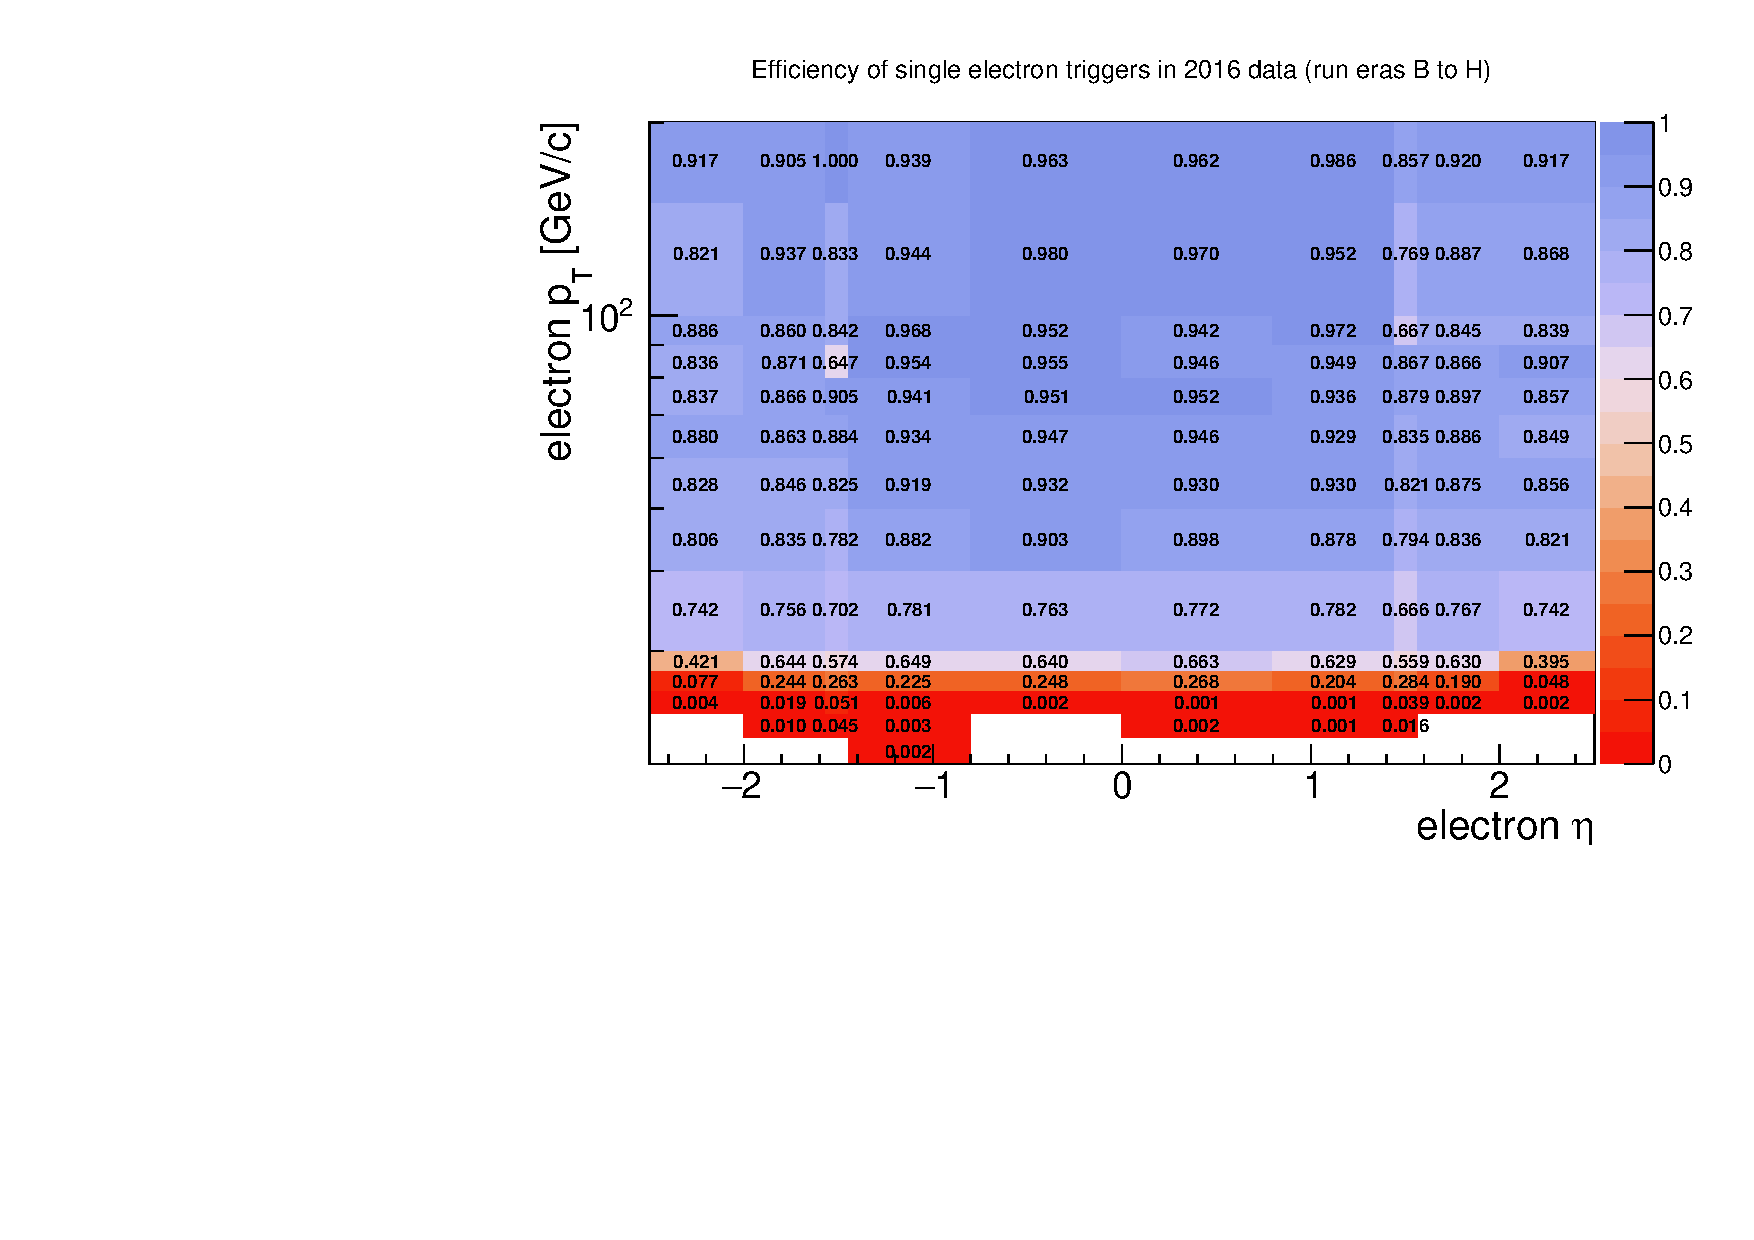
\includegraphics[width=0.75\textwidth]{figures/triggerstudies/singleElectronTrigger_Run2016BCDEFGH.pdf}
       \caption{Measured trigger efficiencies for the single electron triggers in 2016.}
 \label{fig:triggereffal}
 \end{center}
 \end{figure}
\begin{figure}[hbtp]\begin{center}
    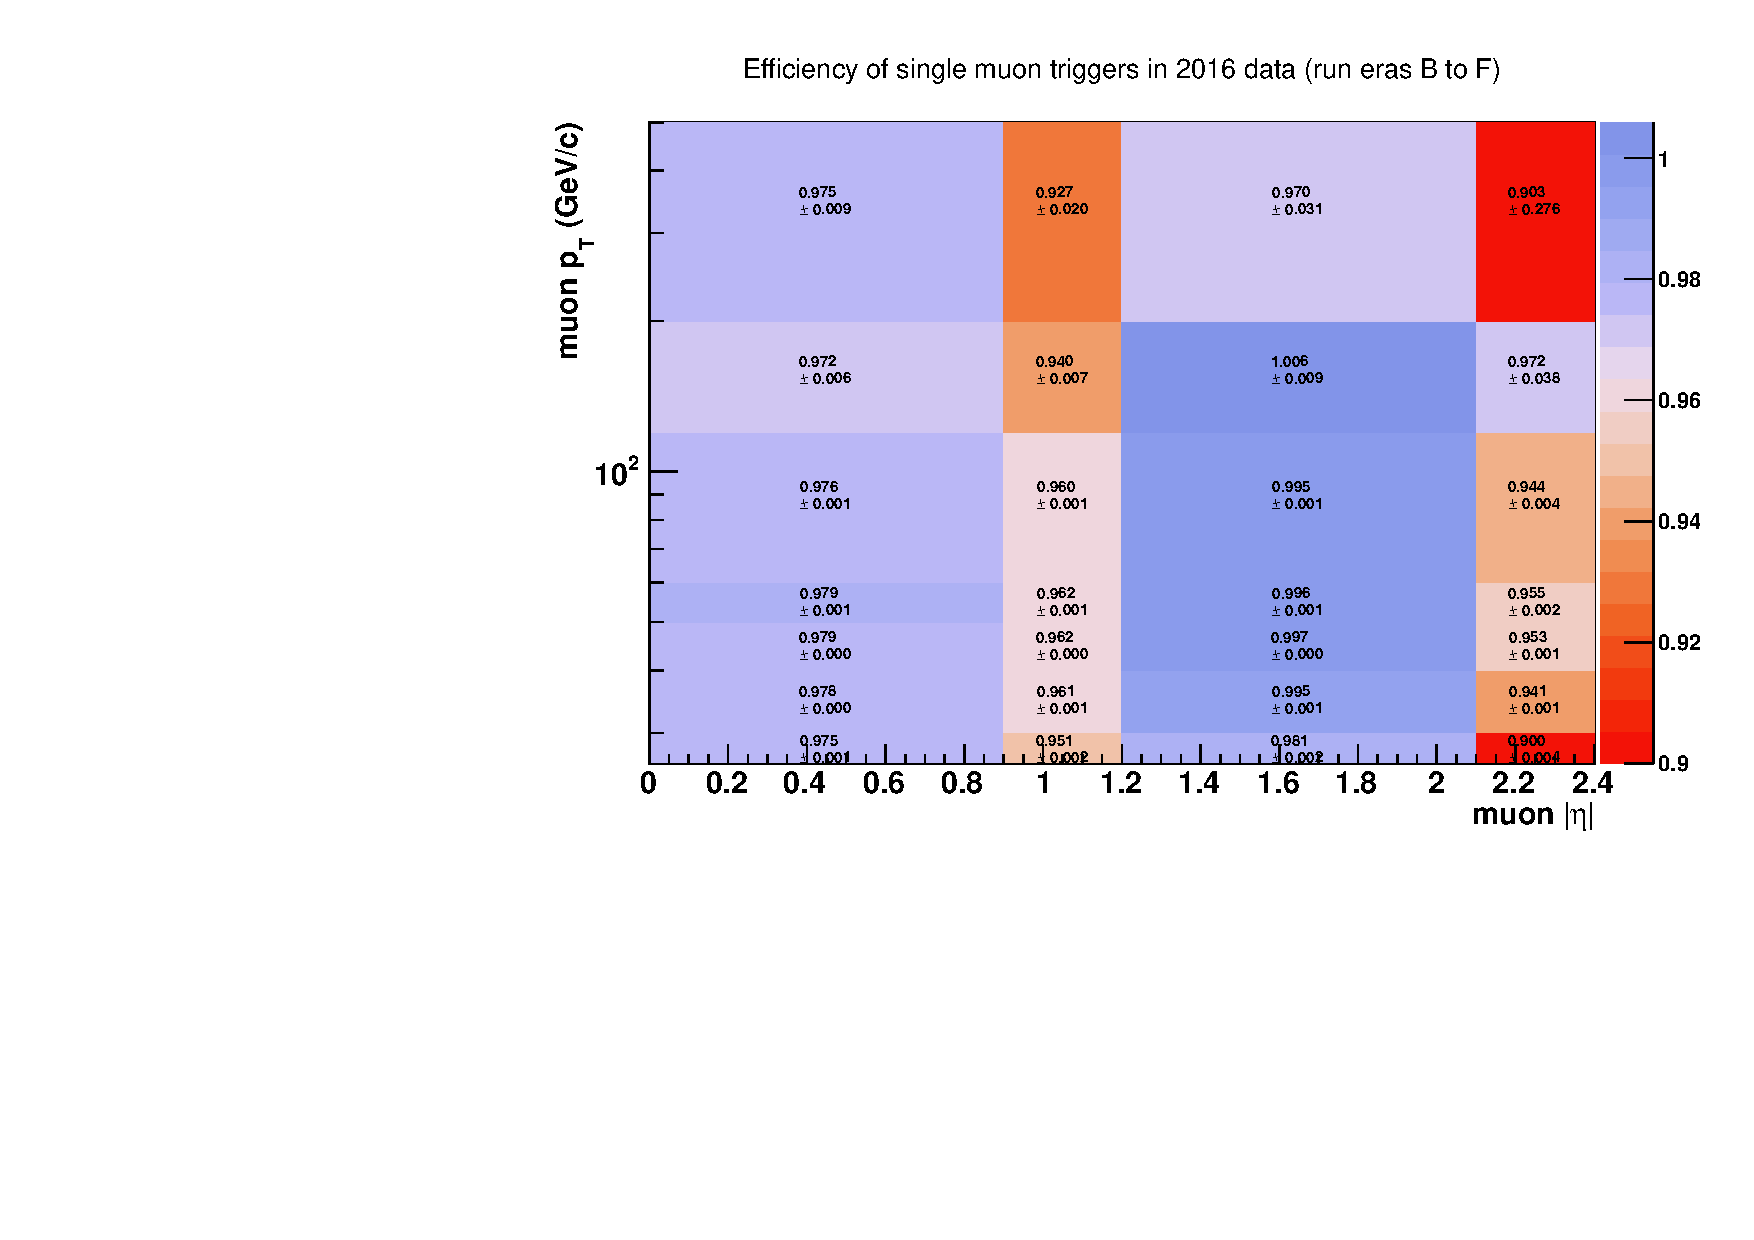
\includegraphics[width=0.75\textwidth]{figures/triggerstudies/singleMuonTrigger_Run2016BCDEF.pdf}
    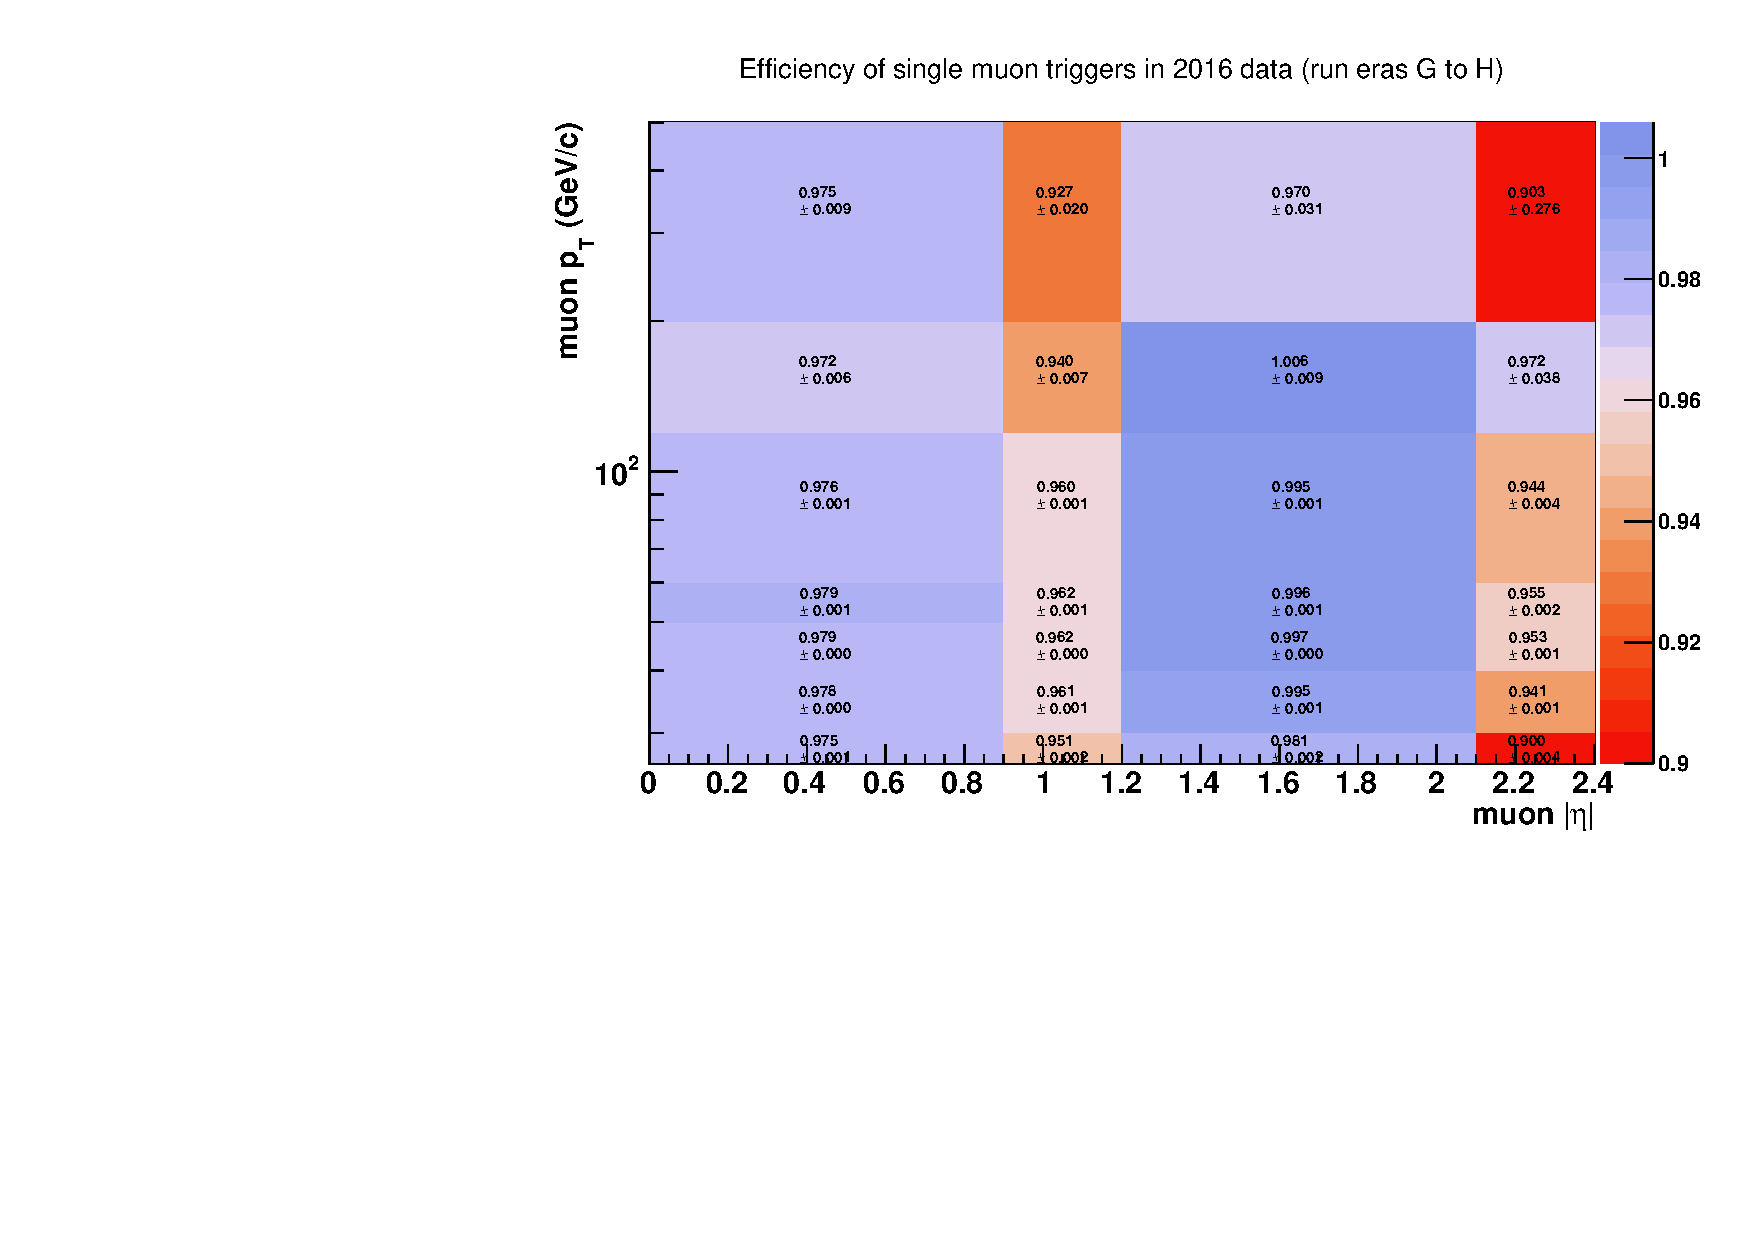
\includegraphics[width=0.75\textwidth]{figures/triggerstudies/singleMuonTrigger_Run2016GH.pdf}
       \caption{Measured trigger efficiencies for the single muon triggers in 2016.}
 \label{fig:triggereffal}
 \end{center}
 \end{figure}


\clearpage
\subsection{Monte-Carlo Simulation}
\label{sec:bkgsamples}

Monte~Carlo samples in CMSSW 80X are taken from the RunIISummer16  productions re-miniAODv2 with the {\it Asympt25ns} conditions. The Spring 2016 In-Time pileup scenario was used to approximate the number of inelastic collisions per bunch crossing at LHC 13 TeV data-taking. Appropriate event re-weighting is applied to reproduce the distribution of the number of primary vertexes in data. 

Samples were produced using one or more of the following programs:
\PYTHIA8~\cite{Sjostrand:2006za,Sjostrand:2007gs}, \POWHEG~\cite{Nason:2004rx}, \TAUOLA~\cite{Golonka:2003xt}, 
and \MADGRAPH5\_aMC@NLO~\cite{Alwall:2011uj,Alwall:2014hca}\
with {\sc MLM} merging~\cite{Mangano:2006rw} or FxFx merging scheme~\cite{Frederix:2012ps}.
Parton shower and hadronisation are performed with \PYTHIA8~\cite{Sjostrand:2007gs} using the CUETP8M1 tune~\cite{Khachatryan:2015pea}.
The {\sc NNPDF3.0} parton distribution functions (PDF)~\cite{Ball:2014uwa} are used for all samples.

The production cross sections for \PW+jets and Z+jets are rescaled to next-to-next-to-leading-order (NNLO)
cross sections calculated using the \FEWZ 3.1 program~\cite{Gavin:2010az,Li:2012wna,Gavin:2012sy}.
These corrections are binned in the generator-level scalar sum of parton $\pt$ (also known as LHE HT),
but we are thinking about ways to do this better.
The $\ttbar$ and single top quark samples are also rescaled to their cross sections based on
NNLO calculations~\cite{Czakon:2013goa, Kidonakis:2012db}.

The WZ and ZZ diboson processes are simulated at next-to-leading order in QCD
The continuum-induced ZZ contribution is neglected due to the small cross section.

The diboson MC samples are generated in electroweak leading-order. For the ZZ
background, a higher order electroweak correction is applied following~\cite{Bierweiler:2013dja,Gieseke:2014gka}  An event-by-event reweighting is performed with correction weights binned in the generator-level \pt of the trailing boson.
This correction results in a net reduction of the overall ZZ yield of about 10\%, although with a strong dependence on the trailing-boson $\pt$.
Overall, the $\pt$ spectrum becomes softer, with a correction of down to $-40\%$ for a trailing-Z $\pt$ of 700~$\GeV$. 
Following~\cite{Baglio:113005}, the corresponding NLO EWK correction to WZ production is small.

Furthermore, for the $\Pq\Pq \to $ZZ process, a QCD NLO to NNLO correction factor is
applied as a function of generator-level invariant mass of the two Z bosons~\cite{qqzz_kfactor,twiki:HZZ4LnnloZZ,talk:SperkaZZcorr}. 
In the case of the WZ process, a NLO to NNLO correction factor of 1.109 is applied~\cite{1604.08576}.

%A list of all background MC samples and the corresponding cross sections are given in Table~\ref{tab:bgmc}.  

\begin{table}[htbp]
\centering 
\resizebox{\textwidth}{!}{
  \begin{tabular}{l|c}
  \hline
  Dataset name & $\sigma$ [pb] \\
  \hline
  /DYJetsToLL\_M-50\_HT-100to200\_TuneCUETP8M1\_13TeV-madgraphMLM-pythia8        & 147.40   \\
  /DYJetsToLL\_M-50\_HT-200to400\_TuneCUETP8M1\_13TeV-madgraphMLM-pythia8        & 40.99    \\
  /DYJetsToLL\_M-50\_HT-400to600\_TuneCUETP8M1\_13TeV-madgraphMLM-pythia8        & 5.678    \\
  /DYJetsToLL\_M-50\_HT-600to800\_TuneCUETP8M1\_13TeV-madgraphMLM-pythia8        & 1.367    \\
  /DYJetsToLL\_M-50\_HT-800to1200\_TuneCUETP8M1\_13TeV-madgraphMLM-pythia8       & 0.6304   \\
  /DYJetsToLL\_M-50\_HT-1200to2500\_TuneCUETP8M1\_13TeV-madgraphMLM-pythia8      & 0.1514   \\
  /DYJetsToLL\_M-50\_HT-2500toInf\_TuneCUETP8M1\_13TeV-madgraphMLM-pythia8       & 0.003565 \\
  \hline
  /WJetsToLNu\_HT-100To200\_TuneCUETP8M1\_13TeV-madgraphMLM-pythia8              & 1343     \\ 
  /WJetsToLNu\_HT-200To400\_TuneCUETP8M1\_13TeV-madgraphMLM-pythia8              & 359.6    \\ 
  /WJetsToLNu\_HT-400To600\_TuneCUETP8M1\_13TeV-madgraphMLM-pythia8              & 48.85    \\ 
  /WJetsToLNu\_HT-600To800\_TuneCUETP8M1\_13TeV-madgraphMLM-pythia8              & 12.05    \\ 
  /WJetsToLNu\_HT-800To1200\_TuneCUETP8M1\_13TeV-madgraphMLM-pythia8             & 5.501    \\ 
  /WJetsToLNu\_HT-1200To2500\_TuneCUETP8M1\_13TeV-madgraphMLM-pythia8            & 1.329    \\ 
  /WJetsToLNu\_HT-2500ToInf\_TuneCUETP8M1\_13TeV-madgraphMLM-pythia8             & 0.03216  \\ 
  /WBJetsToLNu\_Wpt-100to200\_TuneCUETP8M1\_13TeV-madgraphMLM-pythia8            & 6.004    \\ 
  /WBJetsToLNu\_Wpt-200toInf\_TuneCUETP8M1\_13TeV-madgraphMLM-pythia8            & 0.8524   \\ 
  /WJetsToLNu\_BGenFilter\_Wpt-100to200\_TuneCUETP8M1\_13TeV-madgraphMLM-pythia8 & 71.77    \\ 
  /WJetsToLNu\_BGenFilter\_Wpt-200toInf\_TuneCUETP8M1\_13TeV-madgraphMLM-pythia8 & 3.027    \\ 
  \hline
  /ZJetsToNuNu\_HT-100To200\_13TeV-madgraph                                      & 280.5    \\ 
  /ZJetsToNuNu\_HT-200To400\_13TeV-madgraph                                      & 77.7     \\ 
  /ZJetsToNuNu\_HT-400To600\_13TeV-madgraph                                      & 10.71    \\ 
  /ZJetsToNuNu\_HT-600To800\_13TeV-madgraph                                      & 2.562    \\ 
  /ZJetsToNuNu\_HT-800To1200\_13TeV-madgraph                                     & 1.183    \\ 
  /ZJetsToNuNu\_HT-1200To2500\_13TeV-madgraph                                    & 0.286    \\ 
  /ZJetsToNuNu\_HT-2500ToInf\_13TeV-madgraph                                     & 0.006945 \\ 
  \hline
  \end{tabular}}
  \caption{List of background MC samples for the V+jets process. Datasets are LO in QCD and EWK, but will have NLO corrections applied.}
  %Cross-sections marked with $\dag$ are (N)NLO
  \label{tab:vjets_mc}
\end{table}

\begin{table}[htbp]
\centering 
\resizebox{\textwidth}{!}{
  \begin{tabular}{l|c}
  \hline
  Dataset name & $\sigma$ [pb] \\
  \hline
  /ST\_tW\_antitop\_5f\_inclusiveDecays\_13TeV-powheg-pythia8\_TuneCUETP8M1                  & 35.85    \\
  /ST\_tW\_top\_5f\_inclusiveDecays\_13TeV-powheg-pythia8\_TuneCUETP8M1                      & 35.85    \\
  /ST\_t-channel\_antitop\_4f\_inclusiveDecays\_13TeV-powhegV2-madspin-pythia8\_TuneCUETP8M1 & 80.95    \\
  /ST\_t-channel\_top\_4f\_inclusiveDecays\_13TeV-powhegV2-madspin-pythia8\_TuneCUETP8M1     & 136.02   \\
  \hline
  /TTTo2L2Nu\_TuneCUETP8M2\_ttHtranche3\_13TeV-powheg-pythia8                                & 88.288   \\
  /TT\_TuneCUETP8M2T4\_13TeV-powheg-pythia8                                                  & 831.76   \\
  \hline
  /QCD\_HT100to200\_TuneCUETP8M1\_13TeV-madgraphMLM-pythia8                                  & 27990000 \\  
  /QCD\_HT200to300\_TuneCUETP8M1\_13TeV-madgraphMLM-pythia8                                  & 1735000  \\  
  /QCD\_HT300to500\_TuneCUETP8M1\_13TeV-madgraphMLM-pythia8                                  & 366800   \\  
  /QCD\_HT500to700\_TuneCUETP8M1\_13TeV-madgraphMLM-pythia8                                  & 29370    \\  
  /QCD\_HT700to1000\_TuneCUETP8M1\_13TeV-madgraphMLM-pythia8                                 & 6524     \\  
  /QCD\_HT1000to1500\_TuneCUETP8M1\_13TeV-madgraphMLM-pythia8                                & 1064     \\  
  /QCD\_HT1500to2000\_TuneCUETP8M1\_13TeV-madgraphMLM-pythia8                                & 121.5    \\  
  /QCD\_HT2000toInf\_TuneCUETP8M1\_13TeV-madgraphMLM-pythia8                                 & 25.42    \\  
  \hline
  \end{tabular}}
  \caption{List of background MC samples for the top and QCD backgrounds.}
  %Cross-sections marked with $\dag$ are (N)NLO
  \label{tab:vjets_mc}
\end{table}

\begin{table}[htbp]
\centering 
\resizebox{\textwidth}{!}{
  \begin{tabular}{l|c}
  \hline
  Dataset name & $\sigma$ [pb] \\
  \hline
  /WWTo2L2Nu\_13TeV-powheg                             & 12.178  \\ 
  /WWTo4Q\_13TeV-powheg                                & 51.723  \\ 
  /WWToLNuQQ\_13TeV-powheg                             & 49.997  \\ 
  /WZTo1L1Nu2Q\_13TeV\_amcatnloFXFX\_madspin\_pythia8  & 10.71   \\   
  /WZTo1L3Nu\_13TeV\_amcatnloFXFX\_madspin\_pythia8    & 3.033   \\   
  /WZTo2L2Q\_13TeV\_amcatnloFXFX\_madspin\_pythia8     & 5.595   \\   
  /WZTo3LNu\_TuneCUETP8M1\_13TeV-powheg-pythia8        & 4.430   \\ 
  /ZZTo2L2Nu\_13TeV\_powheg\_pythia8                   & 0.5644  \\  
  /ZZTo2L2Q\_13TeV\_amcatnloFXFX\_madspin\_pythia8     & 3.22    \\   
  /ZZTo4L\_13TeV\_powheg\_pythia8                      & 1.212   \\  
  /ZZTo2Q2Nu\_13TeV\_amcatnloFXFX\_madspin\_pythia8    & 4.072   \\
  /ZZTo4Q\_13TeV\_amcatnloFXFX\_madspin\_pythia8       & 6.842   \\   
  \hline
  \end{tabular}}
  \caption{List of background MC samples for the diboson backgrounds. All samples that could have the VZ(bb) final state are simulated at NLO in QCD and LO in EWK, but will be corrected later.}
  %Cross-sections marked with $\dag$ are (N)NLO
  \label{tab:vjets_mc}
\end{table}
\begin{table}[htbp]
\centering 
\resizebox{\textwidth}{!}{
  \begin{tabular}{l|c}
  \hline
  Dataset name & $\sigma$ [pb] \\
  \hline
/WplusH\_HToBB\_WToLNu\_M125\_13TeV\_powheg\_pythia8   &  0.159  \\  
/WminusH\_HToBB\_WToLNu\_M125\_13TeV\_powheg\_pythia8  &  0.100  \\ 
  \hline
  \end{tabular}}
  \caption{List of signal MC samples. Cross sections are taken from the LHC Higgs Cross Section Working Group Yellow Report.}
  %Cross-sections marked with $\dag$ are (N)NLO
  \label{tab:signal_mc}
\end{table}

\subsubsection{\ttbar \pt corrections}
\label{sec:ttbarpt}
Correction factors are applied to the $\ttbar$ sample based on the $\pt$
re-weighting procedure recommended by the Top PAG and based on the
results of Ref.~\cite{CMS-PAS-TOP-16-011} and Ref.~\cite{Khachatryan:2016mnb}. The recommended
scale factor is~\cite{CMS-TOP-PT-REWEIGHT}
\begin{equation}
\mathrm{SF}(\pt) = e^{0.0615-0.0005\cdot \pt}~,
\end{equation}
with the overall event weight given by
$w=\sqrt{SF(\PQt)SF(\cPaqt)}$. The fit for the scale factor function is shown in
Fig.~\ref{fig:topPt}. 
\begin{figure}[hbtp]\begin{center}
    \includegraphics[width=0.45\textwidth]{figures/TopPt_DATA_PWHGP8.pdf}
    \caption{Top \pt reweighting function}
 \label{fig:topPt}
 \end{center}
 \end{figure}

\subsubsection{Higgs \pt for gluon fusion production}
\label{sec:signalpt}

%The normalization of the ggH process is obtained by accounting for the impact, at the level of inclusive rates and of differential \pt distribution, of the merging of samples characterised by different final-state multiplicities, and of the effects induced by top and bottom masses through heavy-quark loop diagrams. Both the merging and the heavy-quark masses must be included in the calculation in order to realistically predict the Higgs boson \pt~\cite{Frederix:2016cnl}. The impact of merging is dominant, but in kinematic regions dominated by large-\pt emissions, mass effects are not negligible but they can be factorized from the NLO corrections. For boosted Higgs production the effect of a finite top mass is well known: adding jets to the hard process pushes one or two gluon propagators off their respective mass shell~\cite{Buschmann:2014sia}, so matrix elements for Higgs production in association with one jet and two jets develop a top mass dependence~\cite{Buschmann:2014sia}. Top mass effects factorize for each number of hard jets to leading order and next-to-leading order, allowing to combine Higgs production in association with one and with two hard jets to optimally probe the structure of the Higgs–gluon coupling~\cite{Buschmann:2014sia}.
%The total cross section for H$+$jet production receives moderate NNLO QCD corrections. For jets defined with the anti-k$_{\rm T}$ algorithm with \pt $>$ 30~\GeV, NNLO QCD corrections are of the order of 20\% for $\mu={\rm m_{H}}$~\cite{Boughezal:2015dra}.
%(NNLO) increase with respect to LO of 44% (72%) for µ = mH and of 25% (31%) for µ = mH/2.
%We adopt a $k$-factor of 1.5 from the N3LO corrections (missing ref?) to normalize the ggH production cross section.


Computing the Higgs boson \pt for the gluon fusion production mode in the region of interest for the analysis poses a number of additional challenges. At low Higgs \pt dominant contributions come from the application of higher order corrections. When going from the leading order (LO) to the next to leading order (NLO) cross section, an increase of 60\% is present. Once this is extended to the highest order, currently ${\rm N^{3}LO}$ the cross section increase is more than a factor of 2. The reason for such a large increase in the production cross section results form the fact that the production is loop induced, which implies the process is very sensitive to higher order corrections. Loop induced processes must further deal with additional modifications at points where the energy scale of the loop becomes resolved. For Higgs production, this occurs at twice the mass of the particles that yield the dominant contribution in the loop, namely the bottom and top quarks. The addition of the low mass b quarks in the loop has the effect of sculpting the \pt distribution at the low end, extending up to $50\GeV$. The resolution of the top loop occurs at a $\pt$ of roughly $350\GeV$. For $\pt$ values above twice the top quark mass, the gluon fusion is found to be almost exclusively dependent on the top-Higgs coupling.  This Higgs \pt distribution is modified by the resolved loop inducing an additional deficit in the production of Higgs bosons at high \pt relative to the case where the loop is unresolved (the so-called Higgs EFT or $m_{\cPqt}\rightarrow\infty$ approximation). 

To account for both the effects of higher order corrections and for the finite top mass loop we incorporate a multi-correction approach. This approach follows a variation of previously work from both \SHERPA and \MCATNLO authors~\cite{Buschmann:2014sia,Frederix:2016cnl}.  

The dominant correction at large values of the Higgs $\pt$ originates from the finite top mass corrections to the loop induced processes. These can be produced at leading ``loop'' (Order) for the 0,1, and 2 jet Higgs production using the loop$_{\rm sm}$ model. Samples are generated with a jet threshold of $20\GeV$ and then showered under various showering scheme. 

In order to validate the generation and showering of the loop induced Higgs production we consider several different showering schemes. For each of these schemes we use inclusively generated finite-top loop Higgs production as obtained from \MCATNLO. First, we consider the CMS default MLM merging here we using a merging scale of $\pt=30\GeV$. Secondly, we consider MLM with a modified scheme for showering. In particular the parameter JetMatching:exclusive is set to zero, which can induce double counting of parameters. Thirdly, we consider default configuration for CKKW showering. In previous studies, CKKW has been chosen as the default showering scheme\cite{Buschmann:2014sia}; following the reference it may have some advantages in phase coverage.  Finally, we consider the inclusive showering of a specified matrix element using the Pythia default showering scheme. The choice of these four different configurations allow for an additional gain in confidence since their production should be roughly the same. 

Figure~\ref{fig:Higgs1j2j} shows the comparison of the Higgs \pt for the 1 and 2 jet production diagrams. From the diagrams we observe the expected scaling whereby the MLM contribution from the 1jet dominates where as the CKKW contribution comes mainly form the higher multiplicity 2jet final state. In each case, we find the respective production matches the inclusively showered production for the 1jet or 2jet final state considering MLM or CKKW respectively. Figure~\ref{fig:HiggsMerge} shows the summed \pt distributions compared with each other and with the two jet inclusive shower. Since we are concerned with very high jet \pt the inclusive 2jet should roughly cover the allowed phase space that is considered. From this plot, we conclude that the modified MLM and CKKW approaches along with the inclusively showered two jet production give a consistent Higgs \pt. We thus, use the CKKW merged sample as a comparison with additional generators. We treat this showered generator as the baseline leading order finite top mass generator for which we compare with the other respective generators.  

\begin{figure}[hbtp]\begin{center}
    \includegraphics[width=0.45\textwidth]{figures/higgspt/Merge_1j.png}
    \includegraphics[width=0.45\textwidth]{figures/higgspt/Merge_2j.png} \\
    \caption{Comparison of the Higgs \pt for (left) 1jet and (right) 2jet samples showered under 4 separate configurations: the Pythia default shower (Inc.), CMS default MLM showering, a modified MLM showering, and finally CKKW-L showering.} 
 \label{fig:Higgs1j2j}
 \end{center}
 \end{figure}

\begin{figure}[hbtp]\begin{center}
    \includegraphics[width=0.65\textwidth]{figures/higgspt/Merged_inc.png}
    \caption{Comparison of the summed 1jet and 2jet samples for loop induced Higgs production with the finite top mass taken into account. Additionally, the 2jet matrix element Higgs \pt is shown where the Pythia default showering is used.  }
 \label{fig:HiggsMerge}
 \end{center}
 \end{figure}

Figure~\ref{fig:Higgskfactor} compares the baseline madgraph generator with the two available generations in CMS. The first is CMS default \POWHEG production. The \POWHEG sample is generated with Higgs matrix elements up to 1 jet assuming the infinite top mass approximation (${\rm m_{top}}\rightarrow\infty$). An additional correction to the high \pt is applied through the use of the \emph{h-fact} parameter, which attempts to approximate the finite top mass corrections\cite{Bagnaschi:2015qta}, but is known to under predict at high Higgs \pt due in part to the arbitrary choice of damping and the lack of the second jet emission. Finally, when comparing the distributions we observe agreement within 20\% for all the distributions at 300\GeV. Secondly, we show the \MCATNLO NLO produced Higgs EFT; here merged for 0,1,2 jets with MLM. Both these two generators are normalized to the inclusive ${\rm N^{3}LO}$ cross section. From these distributions, we observe the merged finite to mass gives the smallest prediction. The NLO EFT is roughly 2.5 times larger than the finite top mass at a \pt of 500 \GeV and the \POWHEG is somewhere in between. Note that the EFT and finite top mass plots represent the current highest orders that can be run with a parton shower Monte Carlo. 

\begin{figure}[hbtp]\begin{center}
    %\includegraphics[width=0.45\textwidth]{figures/higgspt/HiggsBest.png}
    \includegraphics[width=0.65\textwidth]{figures/higgspt/HiggsPtAllComp.pdf} 
    \caption{Comparison of the Higgs \pt for a different set of generators as described in the text.}
 \label{fig:Higgskfactor}
 \end{center}
 \end{figure}

When going from the LO with finite top mass or EFT to highest available orders in both we follow two complementary approaches. Firstly, we consider the highest order Higgs+1jet production. This has been done in three separate ways (with and without the n-jettiness scheme) giving a similar order correction in all~\cite{Chen:2014gva,Boughezal:2013uia,Boughezal:2015dra,Boughezal:2015aha}. For each of the three ways, we find a $k$-factor for the NNLO correction with respect to the NLO correction of 1.25$\pm0.15$ which is roughly flat across \pt. We thus apply this scale factor to all predictions. Secondly, we take into account the finite top mass corrections. This we can perform in one of two ways. Take the NLO EFT and correct for LO ratio of finite top mass to that with the absence of the finite top mass~\cite{Chen:2016zka} or conversely, scaling the finite leading order finite top mass sample by the expected NLO/LO correction finite top mass correction\cite{Neumann:2016dny}. This second correction is not the full NLO finite top mass correction, since that correction is currently not available. Instead, it is the approximate NLO finite top mass correction obtained by expanding the EFT in powers of $1/m_{t}$ (NLO*).

The resulting correction of the finite top mass with respect to the EFT is found to be between $0.4$ and $0.65$ at $500 \GeV$~\cite{Chen:2016zka}. For reference, we take a correction of 0.4, since the correction is \pt dependent but we don't have a derivation of the correction beyond 500~\GeV. The correction for the NLO finite top mass with respect to the leading order is found to be $2.0\pm0.5$ and flat as a function of $\pt$. Finally, we compare these two distributions in figure~\ref{fig:Higgskfactor}. We find the two distributions cross at a $\pt$ near $600\GeV$ with the two predictions within 10\% of each other. The cross is expected since the finite top mass correction to the EFT  will shrink at higher \pt making the EFT an over prediction at the highest \pt. We thus use the NLO* corrected finite top mass as the default spectra. The resulting $k$-factor with respect to the default \POWHEG is found to be $1.6\pm0.48$ at $500 \GeV$. We adopt a 30\% uncertainty following the addition in quadrature of the NNLO and NLO* uncertainties. The full $k$-factors are summarized in table~\ref{tab:kfactor}. Finally in figure~\ref{fig:Higgskfactor}, we compare this to other predictions from \SHERPA and \MCATNLO.  Both these distributions are extracted from their respective papers. For the \SHERPA distribution an additional correction based on the quoted acceptance of a dilepton selection is applied since their quoted \pt distribution is computed with the $\PH\rightarrow \PW\PW$  after a loose dilepton selection. Additionally, in both cases, we have added the additional NNLO scale factor to the cross section for the \SHERPA and an NNLO $k$-factor for \MCATNLO, although from the inclusive cross section a factor of $1.5$ (NLO) as opposed to $1.5\times1.25$ (NNLO) may be more appropriate to yield the current $N^{3}LO$ prediction. Adding the additional NNLO $k$-factor brings the distribution of the 3 predictions to within 20\% agreement.


In Fig.~\ref{fig:Higgspt}, the corrections are shown along with the corrected Higgs \pt distribution.
%Finally, we would like to mention that we have contacted the authors of ~\cite{Neumann:2016dny} and they are helping us prepare a more robust prediction in our phase space. 

\begin{table}[htbp]
\topcaption{Higgs $k$-factors}
\resizebox{\textwidth}{!}{
\begin{tabular}{llll}
\hline
Sample & Yield ($fb^{-1}$)& Order & $k$-factor to \POWHEG \\
 & (\pt$>500~\GeV$)  & \\
\hline
{\small CMS default \POWHEG } & 12.5   & NLO &  1\\
{\small NLO EFT NNLO $k$-factor Mass corr  } & 28.9,36.1,$19^{+5}_{-4}$  & NLO,NNLO,NNLO+m$_{t}$ &  1.5$\pm$0.4\\
{\small LO $m_{t}$ NNLO and NLO* $k$-factor} & 7.8,15.6,$19.5^{+6}_{-6}$ & LO,NLO*,NNLO+m$_{t}$ &  1.6$\pm$0.5\\
\hline
\end{tabular}}
\label{tab:kfactor}
\end{table}

\begin{figure}[hbtp]\begin{center}
    \includegraphics[width=0.7\textwidth]{figures/Hptspectrumcorrected.pdf}
\caption{Generator level Higgs \pt distribution for the gluon fusion production mode. The CMS default \POWHEG sample and the corrected spectrum to account for both higher order and finite top mass effects are compared.}
 \label{fig:Higgspt}
 \end{center}
 \end{figure}


%%% Old crap
%Figure~\ref{fig:higgspt} shows the resulting comparison of the showered Higgs \pt with the default \POWHEG and additional models from the \SHERPA authors~\cite{Buschmann:2014sia}, the Madgraph authors~\cite{Frederix:2016cnl}. Both these distributions are extracted from their respective papers. For the \SHERPA distribution an additional correction based on the quoted acceptance of a dilepton selection is applied since their quoted \pt distribution is computed with the ${\rm H\rightarrow WW}$  after a loose dilepton selection. Finally, we present two additional distributions $\phi_{{\rm matched}}$ which corresponds to the dark matter scalar simplified model of a mediator decaying to b-quarks produced by loop-induced process and corrected for the branching ratios. Secondly, we present the default \POWHEG distributions. When comparing to the default \POWHEG sample, we observe a scale factor of 1.5 for $\pt^{\PH} > 500 \GeV$. In addition to the correction of 1.5 for using the second jet merged sample, an additional correction corresponding the NLO 1 and 2-jet sample is applied on top of the merged sample. This factor of 1.5 can be obtained from the calculation of the inclusive cross section in the \MCATNLO relative to the ${\rm N^{3}LO}$ cross section~\cite{deFlorian:2016spz}. It is additionally derived for the specific jet bins in the \SHERPA paper. Figure~\ref{fig:higgspt} also shows the impact of the additional 1.5 $k$-factor. The combined $k$-factors give a total increase in cross section of $2.36$ for a Higgs \pt$> 500$\GeV. Some care has to be taken for these corrections since the fundamental process is still leading order, which gives an uncertainty of potentially O(50\%) on the total production. 

%\begin{figure}[hbtp]\begin{center}
%    \includegraphics[width=0.45\textwidth]{figures/higgspt/higgspt_nokfactor.png}
%    \includegraphics[width=0.45\textwidth]{figures/higgspt/higgspt_kfactor.png} \\
%    \caption{Comparison of the Higgs \pt for a different set of generators where the NLO $k$-factor is \emph{not} applied (left) and the NLO $k$-factor is applied (right)} 
% \label{fig:higgspt}
% \end{center}
% \end{figure}


\subsubsection{Higgs \pt for VBF}
The Higgs \pt spectrum for the VBF production mode is reweighted to account for higher order (${\rm N^{3}LO}$) corrections to the cross section. The ${\rm N^{3}LO}$ \pt spectrum is shown in Fig.~\ref{fig:VBFpt} and compared to the lowest order calculations. The impact of the highest order corrections to LO is within few\% at high \pt. This is from private communication with the authors of this paper~\cite{Cacciari:2015jma}. The corrections have negligible effect to the yield for this process in the phase space selected by requiring \pt$>450$~\GeV. 

\begin{figure}[hbtp]\begin{center}
    \includegraphics[width=0.7\textwidth]{figures/ptH-log.pdf}
    \caption{Comparison of the Higgs \pt for different order of corrections to the VBF cross section.}
 \label{fig:VBFpt}
 \end{center}
 \end{figure}




\clearpage
\section{Object reconstruction}
\label{sec:physobj}
%%%%%%%%%%%%%%%%%%%%%%%%%%%%%%%%%%%%%%%%%%%%%%%%%%%%%%%%%%%%
%\subsection{Physics Objects}

\subsection{Leptons}
There are four tiers of lepton selections used in this analysis.
\begin{itemize}
  \item Inclusive selection for jet regression 
  \item Selection for jet cleaning
  \item Loose selection for Z boson reconstruction and additional lepton veto
  \item Tight selection for single lepton triggers and W boson reconstruction
\end{itemize}
\subsubsection{Electrons}
  Electrons are reconstructed with the Gaussian Sum Filter
  algorithm (GSF Electrons)~\cite{Khachatryan:2015hwa}. A tighter identification is then applied using a multivariate approach
  recommended by the electron-gamma (EGM) POG as documented here:

  \small{\texttt{https://twiki.cern.ch/twiki/bin/viewauth/CMS/ \\
  MultivariateElectronIdentificationRun2}}.
 
  A dedicated multivariate discriminator is trained for electrons that pass a set of cuts meant to reproduce
  the detector cuts applied by the most common electron triggers. 
  In this case, a set of offline cuts on ECAL-based electron quantities is applied
  on top of the multivariate discriminator to reproduce the conditions of the training sample:

  \texttt{pt>15 \& (}\\
  \texttt{(abs(superCluster().eta)<1.4442 \& full5x5\_sigmaIetaIeta<0.012 \& }\\
  \texttt{hcalOverEcal<0.09 \&}\\
  \texttt{(ecalPFClusterIso/pt)<0.4 \& (hcalPFClusterIso/pt)<0.25 \&}\\
  \texttt{(dr03TkSumPt/pt)<0.18 \& abs(deltaEtaSuperClusterTrackAtVtx)<0.0095 \&}\\
  \texttt{abs(deltaPhiSuperClusterTrackAtVtx)<0.065) || }\\
  \texttt{(abs(superCluster().eta)>1.5660 \& full5x5\_sigmaIetaIeta<0.033 \&}\\
  \texttt{hcalOverEcal<0.09 \&}\\
  \texttt{(ecalPFClusterIso/pt)<0.45 \& (hcalPFClusterIso/pt)<0.28 \&}\\
  \texttt{(dr03TkSumPt/pt)<0.18)}\\
  \texttt{).}

  Two cuts on the MVA ID discriminator~\cite{MVAeID} are applied
  defining two different working points based on the expected selection efficiency
  of either $90\%$ (loose, WP90) or $80\%$ (tight, WP80). The MVA working points are for the Spring 2016 training.
  
  \textbf{Inclusive selection for jet regression}: Electrons found inside jets are used to train the b-jet energy regression.
  We consider electrons for the quantities related to the leptons in jets,
  if they have $\pt > 5 \GeV$, $d_{xy}<0.5\cm$, $d_z<1.0\cm$, and no more than one expected missing
  inner tracker hits. 
  This selection is grandfathered in from the 76X Heppy framework for synchronization reasons,
  and should be reworked for the legacy analysis.
  More specifically, the GSF electron efficiency is known to drop substantially within heavy flavor jets
  due to the saturation of the ECAL, and most of the electrons selected this way are fakes.
  
  \textbf{Selection for jet cleaning}:
  Electrons are selected for jet cleaning by requiring $\pt>7\GeV$, $|\eta|<2.4$, $d_{xy}<0.05\cm$, $d_z<0.2\cm$ 
  (where both distances are taken with respect to the primary vertex), and a very loose relative
  isolation cut of 0.4, where the $\rho$-subtracted PF isolation in a cone of radius $0.3$ is used (Sec.~\ref{sec:leptiso}).
  The EGM scale corrections are currently applied to the electron $\pt$ before calculating this relative isolation.
  This is apparently not what was implemented in the 76X Heppy framework.

  \textbf{Loose selection}:
  Electrons which pass the Loose WP90 MVA working point are used to reconstruct Z bosons and for vetoing on additional leptons.
  The leading electron for Z boson reconstruction must have $\pt > 20\GeV$ for trigger threshold reasons.
  Otherwise, the electrons with $\pt > 15\GeV$ are used for the additional lepton veto.

  \textbf{Tight selection}:
  The tighter WP80 MVA working point is used in the \WenH\ channel to suppress the fake background in
  that final state. The tight electrons must also $\pt > 30\GeV$ and relative isolation $< 0.06$.
  To be clear, the same relative isolation and $\pt$ assignment are used as in the "Selection for jet cleaning."
  %in the \WenH\ and \ZeeH\ analyses, respectively, for the leading lepton. In the \ZeeH channel,
  %the trailing lepton is required to have $\pt$ in excess of $15\GeV$

\subsubsection{Muons}
  \textbf{Inclusive selection for jet regression:}:
  Muons found inside jets are also used to train the b-jet energy regression.
  We consider PF and global muons for the quantities related to the leptons in jets,
  if they have $\pt > 3 \GeV$, $d_{xy}<0.5\cm$, and $d_z<1.0\cm$.
  
  \textbf{Selection for jet cleaning}:
  The muons chosen for jet cleaning are PF muons reconstructed as either global or tracker muons, having $\pt>5\GeV$, $|\eta|<2.4$, $d_{xy}<0.5\cm$, $d_z<1.0\cm$, and
  relative isolation $< 0.4$, where the $\Delta\beta$-subtracted PF isolation in a cone of radius $0.4$ is used.

  \textbf{Loose selection}:
  The selection of muons for the Z boson reconstruction and the additional lepton veto is the same as
  the selection for jet cleaning, except that the leading (subleading) muon for Z boson
  reconstruction must have $\pt > 20 (10)\GeV$ for trigger threshold reasons.

  \textbf{Tight selection}:
  The tight muon selection is used in the \WmnH\ channel.
  It comprises muons having $\pt > 25\GeV$ and relative isolation $< 0.06$,
  which pass the following standard Tight ID cuts which have not changed since 2012:
 \begin{itemize}
  \item the candidate is reconstructed as a Global Muon:\\
  \texttt{isGlobalMuon()}
  \item Particle-Flow Muon:\\
  \texttt{isPFMuon()}
  \item $\chi^2/ndof$ of the global-muon track fit:\\
   \texttt{globalTrack()->normalizedChi2() < 10.}
  \item at least one muon-chamber hit included in the global-muon track fit:\\
  \texttt{globalTrack()->hitPattern().numberOfValidMuonHits() > 0 }
  \item muon segments in at least two muon stations; this implies that the muon is also an arbitrated tracker muon:\\
  \texttt{numberOfMatchedStations() > 1 }
  \item tracker track transverse impact parameter w.r.t. the primary vertex:\\
  \texttt{fabs(muonBestTrack()->dxy(vertex->position())) < 0.2 }
  \item longitudinal distance of the tracker track wrt. the primary vertex:\\
  \texttt{ fabs(muonBestTrack()->dz(vertex->position())) < 0.5 }
  \item number of pixel hits:\\
  \texttt{ innerTrack()->hitPattern().numberOfValidPixelHits() > 0 }
  \item cut on number of tracker layers with hits:\\
  \texttt{innerTrack()->hitPattern().trackerLayersWithMeasurement() > 5}
 \end{itemize}
  
\subsubsection{Lepton isolation\label{sec:leptiso}}

 Lepton isolation is defined starting from the PF isolation equation:
\begin{linenomath}\begin{equation}
  R\equiv \frac{\sum_i \left [ {\pt}_i(\texttt{chargedHadron}) + {\pt}_i(\texttt{neutralHadron}) + {\pt}_i(\texttt{Photon}) \right ]}{{\pt}^{\Pgm}}
\end{equation}\end{linenomath}

adding a term for subtraction of PU energy and momentum.  
This subtraction is based on the per-event estimated neutral energy expected to enter
a cone of radius $0.3$ ($0.4$) around the electron (muon) momentum. 
For electrons the estimate is obtained by computing the standard $\rho$ variable
using only neutral particle flow objects,
and then multiplying by a POG-estimated effective area of the cone (\texttt{Spring15\_25ns\_v1}).
For muons the correction is estimated from the deposit associated to charged tracks not belonging to the
primary vertex, with calibration factors given by the muon POG.   

Although the cuts are tight there is no loss in expected sensitivity and the data/MC agreement is very good in the bulk of the isolation distribution.

\subsection{Jets}

Jets used in the analysis are reconstructed by clustering particle flow candidates in the event using the anti-k$_{\rm T}$ algorithm \cite{Cacciari:2008gp} 
with a distance parameter of 0.4 and 0.8, constituting the AK4 and AK8 fatjets respectively. Details concerning their reconstruction follow.

The latest jet energy corrections are applied to data ({\tt Summer16\_23Sep2016[BCD,E,F,G,H]V3\_DATA}) and MC ({\tt Summer16\_23Sep2016V3\_MC}), following the JME POG recommendations~\cite{CMS-JEC-TWIKI}. 
Since the jet energy resolution (JER) differs in data and MC, in order to get a better agreement an additional smearing is applied to the simulation. The {\tt Spring1625ns\_V10} tag is currently used.

\subsubsection{AK4 Jets}
The official JME ``loose'' PF jet ID and the loose pileup ID are applied to the AK4 jets. We reject a jet if $\Delta {\rm R (jet,l)}<$~0.4 where $l$ is a preselected electron or muon.}

For the resolved categories, AK4 jets with $\pt > 25$ and $|\eta|<2.4$ are considered for building the \HBB system and for counting additional jets.
For the boosted AK8 fatjet categories, we define isolated jets, as AK4 jets with $\pt > 30$, $|\eta|<2.4$, and $\Delta {\rm R}>$~0.8 with respect to the highest
momentum AK8 fatjet. Applying b-tagging to the isolated jets allows us to reject or enhance the top-quark contribution in the signal and control regions.

\subsubsection{AK8 Fatjets}
To mitigate the effect of multiple interactions in the same bunch crossing, the pileup per particle identification (PUPPI) algorithm~\cite{Bertolini:2014bba} 
is used to weight the particle flow candidates prior to clustering the fatjets. This pileup jet discriminator is built based on event pileup properties, local shape and tracking information.
Further corrections are applied as a function of jet pseudorapidity($\eta$) and transverse momentum (L2,L3 corrections) to account for detector non-linearities.
Differences between data and simulation after L2 and L3 corrections are removed by applying a specific calibration to data events. Residual corrections are extracted from data using
the transverse momentum balance in $\gamma$+jets and Z+jets events~\cite{Chatrchyan:2011ds}. These corrections have been computed directly for AK8 PUPPI jets.

Subsequent to the clustering, we apply a jet grooming algorithm called "soft drop" which removes soft and wide-angle contributions from the jet, in order to mitigate the effects of contamination from initial state radiation (ISR), underlying event (UE) and pileup\cite{Larkoski:2014wba}.
Like any grooming method, soft drop declustering removes wide-angle soft radiation from a jet in order to mitigate the effects of contamination from initial state radiation (ISR), underlying event (UE), and multiple hadron scattering (pileup). Given a jet of radius $R_0$ with only two constituents, the soft drop procedure removes the softer constituent unless:

%\begin{linenomath}\begin{equation}
 $$\frac{\min(\pt^1,\pt^2)}{\pt^1+\pt^2} > z_{\mathrm{cut}} \left( \frac{\Delta R_{12}}{R_0} \right)^\beta$$
%\end{equation}\end{linenomath}
This algorithm controls the soft wide-angle radiation by a soft radiation fraction threshold $z_{\mathrm{cut}}$ and an angular exponent parameter $\beta$, where $\beta =0 $ corresponds roughly to the (modified) mass-drop procedure (mMDT) detailed in ~\cite{Dasgupta:2013ihk}. The default parameters used by CMS are $\beta=0$ and $z_{\mathrm{cut}}=1$.
The soft drop algorithm has the benefit of performing jet grooming in a theoretically safer way~\cite{Larkoski:2014wba,Larkoski:2013paa} and its behavior is constant across different clustering distance parameters~$R$ and \pt, which is not true for the pruning technique~\cite{Ellis:2009su,Ellis:2009me}.
Although the soft drop algorithm is primarly aimed at separating boosted \PW-jets from light quark/gluon-jets, it can fully reject contributions from underlying event and pileup when combined with the PUPPI algorithm.

The soft drop jet mass ($\mSD$) is the most important variable in the boosted fatjet categories. 
The $\mSD$ distribution peaks at the H mass for signal events, while the mass of background light quark- and gluon-initiated tends lower. 
The mass of top quark fatjets peaks at either the top quark mass, or the W boson mass if the top's b-quark daughter is not reconstructed inside the fatjet.

Specific corrections to the PUPPI soft drop mass are applied to correct for residual \pt-dependence, evaluated centrally by JMAR and documented in~\cite{AN-16-215}.
\begin{itemize}
  \item {\bf gen corrections}: a \pt-dependent correction to account for a small shift in the generated vector boson mass (derived for boosted W jet)
  \item {\bf reco corrections}: a \pt-dependent correction to the reconstructed jet mass, applied separately for jets in the barrel and endcaps regions
\end{itemize}

The shift in generated softdrop mass at lower \pt is of the order of 2-3\% while the difference between reconstructed and generated softdrop mass is a 5-10\% effect.
The mass shift introduced at generator level is corrected by a fit to $M_\textrm{PDG}/M_\textrm{GEN}$
as a function of jet \pt, where $M_\textrm{PDG} = 80.4$~\GeV and $M_\textrm{GEN}$ is the fitted mean of the generator level mass.
To correct for the residual shift between generator and reconstruction level, a fit to $(M_\textrm{RECO} − M_\textrm{GEN})/M_\textrm{RECO}$,
where $M_\textrm{RECO}$ is the reconstructed jet mass.

\subsubsection{Jet substructure}
\label{sec:substructure}

Jet substructure observables are used to distinguish boosted \PH bosons that decay hadronically from the hadronization products of single light quarks or gluons,
as well as top quarks.
Examples of observables widely used in jet substructure include $N-$~subjettiness ratios~\cite{Thaler:2010tr} and energy correlation functions (ECFs)~\cite{Larkoski:2013eya}.
These are usually constructed using power counting techniques, from a basis of infrared and collinear (IRC)\footnote{A general
IRC safe observable, insensitive to the emission of soft or collinear gluons, can be constructed using all energy deposits and angular information of a hard scattering event.}
safe observables that probe $N-$prong substructure within a jet.
Power counting~\cite{Larkoski:2014gra} can predict which combinations of observables are optimally sensitive to specific parametric features within a jet and can elucidate the underlying physics probed by the observables.

The quantity \textbf{N-subjettiness}~\cite{Thaler:2010tr,Thaler:2011gf,Stewart:2010tn} $\tau_N$ is used to quantify the degree to which jet constituents can be arranged into N subjets. It is defined as:

\begin{equation}
\tau_{N} = \sum_{1 \leq i \leq n_{J}}{z_{i} \min\{\Delta R_{i1}^{\beta},...,\Delta R_{iN}^{\beta}\}},
\end{equation}

where $z_{i}$ refers again to the energy fraction, and $\Delta R_{iK}$ refers to the angular separation between the constituent $i$ and the subjet axis $K$ in the jet. In particular, the ratio of ``$2-$~subjettiness'' to ``$1-$~subjettiness'' ($\tau_{2}/\tau_{1}$ = $\tau_{21}$) is designed to take small values for a jet with well-resolved 2-prong substructure, and has therefore, excellent capability at separating jets originating from boosted vector bosons from jets originating from quarks and gluons. The ratios $\tau_2/\tau_1$ and $\tau_3/\tau_2$ are calculated for the $\PH(\bbbar)$ fatjet, where the latter is aimed at reducing the amount of top quark background.

$N-$~subjettiness~($\tau_{N}$) divides a jet into $N$ sectors and correlates the particles in each sector with their corresponding axis. 
Thus, the definition of N-subjettiness requires an implicit definition of appropriate N-subjettiness axes, which can lead to different behaviors of the observable. In this context,
a new basis of IRC safe observables was recently proposed in~\cite{Moult:2016cvt}. These observables, named as generalized energy correlation functions ($_{o}e_{n}^{\beta}$), are defined as follows:

\begin{equation}
_{o}e_{n}^{\beta} = \sum_{1\leq i_{1}<i_{2}<...<i_{n}\leq n_{J}}{\prod_{1\leq k \leq n}{z_{i_{k}}}} \times \color{black}{\min \{ \prod_{s<t\in \textrm{pairs}\{i_1,i_2,...,i_n\}}^{o} {\Delta R_{st}^{\beta}}\} }\color{black},
\label{eq:ecfs}
\end{equation}

where:

\begin{itemize}
\item $n$, denotes the number of particles to be correlated i.e. the order of the correlation function. For an $n-$~pronged jet, $e_{n} >> e_{m}$, for $m \geq n$.
\item $o$, denotes the order of the angular factor, and
\item $\beta$, is related to the angular weighting.
\end{itemize}

The $_{o}e_{n}^{\beta}$ correlate $o$ pairwise angles among $n$ particles, allowing high flexibility in angular scaling. Furthermore, we define dimensionless ratios of the energy correlation functions as:

\begin{equation}
\psi(a,\alpha,N;b,\beta,M) = \frac{e(a,N,\alpha)}{e(b,M,\beta)^x}\text{, where } M\leq N\text{ and }x=\frac{a\alpha}{b\beta}
\label{eq:psi}
\end{equation}

In the boosted fatjet category of the \WenH\ and \WmnH\ channels, we use several dimensionless ratios of the 4-point and 3-point correlations to separate the \HBB\ signal from 
top quark background in the event classifier BDT.

\subsection{Missing Transverse Energy}

The $\MET$ used in the analysis is computed by taking the negative vector sum of the transverse momenta of all particle flow candidates reconstructed in a given event. Corrections to the momenta of jets reconstructed in the event are further propagated to the $\MET$ (Type-1 corrections).%, weighted with weights calculated by the PUPPI algorithm. Corrections to the momenta of jets reconstructed in the event are further propagated to the $\MET$ (Type-1 corrections).
Events in data can end up with large spurious $\MET$ due do detector noise and beam backgrounds.
In order to remove these events several $\MET$ filters have been recommended by the JetMET POG and have been implemented in the analysis.

\begin{center}

\href{https://twiki.cern.ch/twiki/bin/view/CMS/MissingETOptionalFiltersRun2}{\texttt{https://twiki.cern.ch/twiki/bin/view/CMS/MissingETOptionalFiltersRun2}}

\end{center}


In the \WenH\ and \WmnH\ channels, the $\MET$ is used along with the tight lepton that passes the trigger to build the W boson momentum in the transverse plane.

The significance of the missing transverse energy (METsig) assesses, on an event by event basis, the likelihood that an observed MET is consistent with a fluctuation from zero because of detector-related limitations like finite measurement resolution. The variable is used to reject QCD-like events with no genuine MET:

\begin{center}

\href{https://twiki.cern.ch/twiki/bin/view/CMSPublic/SWGuideMETSignificance}{\texttt{https://twiki.cern.ch/twiki/bin/view/CMSPublic/SWGuideMETSignificance}}

\end{center}

\subsection{B-tagging\label{sec:bjets}}
\subsubsection{CMVA for AK4 jets}
The identification of AK4 jets that originate from the hadronization of $\PQb$ quarks
is done with the Combined MVA v2 (cMVAv2)     algorithm~\cite{Chatrchyan:2012jua} with \texttt{PAT} string:
\begin{center}
\texttt{pfCombinedMVAV2BJetTags}
\end{center}
(while for the previous iteration of the analyses we have instead used the Combined Secondary Vertex CSVv2 algorithm).
The CMVAv2 algorithm provides a continuous discriminator output combining
in an optimal way the information about track impact parameters and identified secondary 
vertices within jets,  even when full vertex information is not available, and information of any soft lepton present in the jet.  Additional
categories for jets where a ``pseudo vertex'' is found, or no vertex at all is identified,
can be defined and combined in a multivariate discriminant (Boosted Decision Tree) to provide maximal separation
of b jets from the much larger background of jets arising from charm decay, and from the
fragmentation of light quarks and gluons.

The CMVAv2 output that can be used to select 
optimal working points with respect to the VH analyses, in addition to the standard 
Loose/Medium/Tight working points defined by the BTV POG: CMVAv2L $(>-0.5884)$, 
CMVAv2M $(>0.4432)$, and CMVAv2T $(>0.9432)$.
Independent optimizations of the selection criteria in all five channels arrive at roughly the same 
optimal selection for the jet in the Higgs decay that has the higher value of the CMVAv2
output: very close to the CMVAv2T working point. For the second jet, the optimal selection 
typically falls between the CMVAv2L and CMVAv2M working points.

The calibration of the CMVAv2 discriminator is determined using a tag-and-probe method
as documented in Ref.~\cite{bTagWeight}.
This method attempts at correcting the distribution of the CMVAv2 discriminator for simulated jets
as to match the distribution observed in data control regions.
These control regions are preselected by the requiring at least two opposite-sign leptons
plus at least two jets. Two exclusive set of selections based on the dilepton mass and the CMVAv2 discriminator or
a ``tag'' jet are further imposed to enrich the control regions in Z+jets or $\mathrm{t\bar{t}}$, respectively.
The binned CMVAv2 distribution of the ``probe'' jet is the compared to the one expected from simulation. An iterative
procedure is then initiated to scale every bin content in the simulation simultaneously for light and heavy flavour jets
(\texttt{hadronFlavour()=0} and \texttt{hadronFlavour()=5}, respectively). This procedure is carried out for various
$\pt$ and $|\eta|$ bins 
The ratio between the re-scaled distribution in the simulated sample and the original one is used as a jet-by-jet 
weight, $w_j$, defined as
\begin{linenomath}\begin{equation}
w_j(\mathrm{CMVAv2}_j;{\pt}_j,|\eta_j|,\mathrm{flavour}_j).
\end{equation}\end{linenomath}
By construction, the weights average to one when sampling CMVAv2 using the distribution predicted by the
simulation: $N^{-1}\sum_{i=1}^{N} w_j \to 1$, for $N>>1$ jets. 
In an event with $N_{\mathrm{jet}}$ selected jets whose CMVAv2 discriminator is used in the analysis,     
an event weight $w$ is defined starting from the jet weights as:
\begin{linenomath}\begin{equation}
w = \prod_{j=1}^{N_{\mathrm{jet}}} w_j(\mathrm{CMVAv2}_j;{\pt}_j,|\eta_j|,\mathrm{flavour}_j).
\end{equation}\end{linenomath}

\subsubsection{Double b-tag for AK8 fatjets}
In order to identify candidate Higgs fatjets containing two b quarks,
we use the double \cPqb-tagger discriminant~\cite{CMS-PAS-BTV-15-002}.

A brief description of the double-b tagger algorithm is as follows:
Tracks and secondary vertices associated to a jet are used, as for standard \cPqb-tagging.
The tracks are used to calculate the axes of N-subjettiness in the fatjet, by defining an axis for each prong which are used as input to the double-b tagger, instead of the jet-direction.
The two $\tau$-axis directions are used to resolve the two B-hadron decay chains we expect for a X to \bbbar\ signal.
Secondary vertex observables are assigned to each axis independently of the subjet components.
Then, b-tagging observables are computed using displaced tracks, secondary vertices (SV), and two-SV system information.
This dedicated tagger represents an alternative for boosted topologies to the subjet b-tag which relies on the subjet definition which breaks down at higher \pt.

For this analysis, we cut on the medium working point of 0.8 to gather events with real boosted \bbbar\ pairs.
The efficiency for passing this cut differs between data and simulation.
This is accounted for by applying a Data/MC scale factor to the efficiency.
The signal scale factor is measured centrally by the BTV POG, and is applied to the efficiency for the true VH(bb) signal,
as well as the highly signal-like \ensuremath{\mathrm{V+\bbbar}}\ backgrounds.
The mistag efficiency scale factors for the \ttbar\ and V+light flavor jets backgrounds are each measured in situ, by
adding to the maximum likelihood fit a Gaussian-constrained nuisance parameter for the simulated efficiency
which is adjusted for the Data/MC discrepancy by an unconstrained nuisance parameter.

The mistag scale factor for \ttbar\ is also measured centrally by the BTV POG, providing a useful cross-check that our
model is correct and unbiased. We measure the \ttbar mistag scale factor to be $\mathbf{1.09 \pm 0.02}$, which is
to be compared with the central numbers $\mathbf{1.05 \pm 0.04}$ (for $\pt < 350 \GeV$) and $\mathbf{1.09 \pm 0.08}$ (for $\pt < 700 \GeV$).
No such cross-check exists for the V+LF mistag scale factor, which is one of the dominant uncertainties in the boosted category.
One way to improve the boosted category sensitivity, if time permits, would be to measure it independently
to provide an initial constraint.

Because the shape of the double b-tag is mismodeled, and corrections for this are not available,
we cannot use the actual discriminator value as an input for the signal extraction BDT.
Future plans including upgrading to a deep neural network implementation for double b-tagging, which was recently integrated centrally in CMSSW.
This can benefit from the same in situ scale factor strategy if the central numbers become available in time.

\subsection{Soft activity calculation}\label{sec:soft}
For the VH signal events, not much additional hadronic activity is expected
after excluding the V and H decay products.
The additional soft activity is defined as follows.
We make only use of charged tracks that clearly originate from the event main interaction point
to monitor the additional radiation.
As described above, the main interaction point in the event is defined as the ``hardest''
reconstructed primary vertex (PV),
i.e. with the largest \pt$^2$ sum for the tracks that have been used to reconstruct it.

At first a collection of soft additional tracks is built using reconstructed tracks that 
\begin{itemize}
\item  have a  {\em high purity} quality flag ,
\item have $\PT>300~\MeVc$,
\item are not associated to the vector decay leptons, nor to the selected two b-jets in the event 
(through the PF candidates components track references),
\item make minimum $|d_z({\rm PV})|$ when associated to the event hardest primary vertex (PV), 
\item satisfy $|d_z({\rm PV})|<$~2~mm with respect to the hardest PV.
\end{itemize}

In addition to removing the tracks in the jets, also tracks in 
the region between the two b-jets are removed by defining a ellipse in 
the $\eta\phi$ plane around the two b-jets with axes $(a,b)= (\Delta R({\rm bb})+1,1)$,
and excluding all tracks pointing within the ellipse from the additional tracks collection.
A schematic of this is shown in Figure~\ref{fig:softActivity}.

\begin{figure}[tbp]
  \begin{center}
    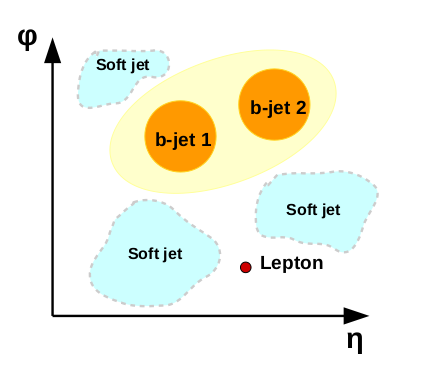
\includegraphics[width=0.48\textwidth]{figures/wlnhbb2016/softActivitySchematic.png}
    \caption{Schematic diagram for the exclusion of tracks for the soft activity calculation.}
    \label{fig:softActivity}
  \end{center}
\end{figure}

After this track selection, a collection of soft track jets is built clustering the aforementioned soft additional tracks
with the anti-$k_{\rm T}$ clustering algorithm~\cite{Cacciari:2008gp} with distance parameter $R=0.4$.
The use of track-jets represents a clean and commissioned method~\cite{CMS-PAS-JME-10-006} to reconstruct
the hadronization of partons with very low energies, down to few GeV~\cite{CMS-PAS-JME-08-001}.

For the purpose of separating the signal from backgrounds, we consider:
\begin{itemize}
\item the scalar $\pt$ sum of the soft track jets with transverse momentum $\pt>1~\GeV$, $H_T^{\rm soft}$; 
\item the soft track jet multiplicity $N^{\rm soft}$ with transverse momentum $\pt>2~\GeV$, $N_2^{\rm soft}$;
\item the soft track jet multiplicity $N^{\rm soft}$ with transverse momentum $\pt>5~\GeV$, $N_5^{\rm soft}$;
\item the soft track jet multiplicity $N^{\rm soft}$ with transverse momentum $\pt>10~\GeV$, $N_{10}^{\rm soft}$;
\end{itemize}

The soft activity is used as a discriminating variable in the signal extraction BDT for the resolved categories.


\subsection{Top(bW) mass reconstruction}\label{sec:topmass}

In the resolved \WlnHbb\ categories,the background from \ttbar\ production is problematic
and grows faster with $\sqrt{s}$ than Higgs boson production.
Therefore, several variables were analyzed to help further discriminate against 
this background. In the end, the reconstructed top mass was included as an 
analysis variable because of its discrimination power.

\WlnHbb\ events are characterized by the presence of an isolated lepton, 
$\MET$, and two b-jets.  This is the same signature for semi-leptonic \ttbar\ 
events.  Furthermore, the lepton and the $\MET$ should both arise from the 
decay of the W boson.  Assuming this W boson is exactly on shell as a constraint,
we solve an equation with lepton \pt\, W mass, known \pt\ of the neutrino 
(assumed to be equal to $\MET$) and unknown longitudinal neutrino momentum.

\begin{eqnarray}
M_{W}^2 & = & (E_{\nu}+E_{\ell})^2-(\overrightarrow{p_{\nu}}+\overrightarrow{p_{\ell}})^2
\end{eqnarray}

There are always two solutions to this equation.  When both are real, the 
solution with the smaller longitudinal neutrino momentum is selected.  When 
the solutions are imaginary, the real part is taken as the longitudinal 
neutrino momentum.

Once this is done, the 4-momenta of the neutrino, the lepton,
and the closest b-jet are added to furnish the top quark's invariant mass.

\clearpage
\section{Event selection}
\label{sec:selection}
\subsection{WH 1-lepton resolved category}
%\begin{table}[tbp]
Events are only analyzed in the boosted category if they have a fatjet and a W boson each with $\pt > 250 \GeV$,
an azimuthal separation of at least 2.5 radians between them, and this fatjet has soft drop mass $\msd > 40 \GeV$.
Otherwise, they are analyzed in the resolved category.
This choice is made to set up the resolved category with the majority of the events,
leaving the boosted category statistically depleted but with higher signal purity.

The \WlnH\ resolved category has one signal region and four control regions.

\textbf{Signal region}: In the signal region, we look for the \HBB\ decay in a dijet system recoiling
back-to-back against a W boson decaying semileptonically. The momenta of both must be greater than 100 \GeV.
Then, we require the tight working point for the higher b-tag score of the two \HBB\ jets to reduce the light flavor backgrounds.
Wwe allow at most 1 additional jet to reduce the \ttbar background.
Finally, the mass window of $[90,150] \GeV$ envelops the Higgs(125) resonance peak.
Blinded plots of analysis variables in this region are shown in Figures~\ref{fig:res_WenSR_WBosons}--\ref{fig:res_WmnSR_WH}.

\textbf{W + light flavor jets region}: Abbreviated \textbf{W+LF}, this control region aims to measure the component of the
W+jets process where the initial state radiation jets produced in association with the W are initiated by u,d,c,s quarks or gluons.
This is done by requiring that the highest b-tag pass the loose, but not the medium working point.
Any number of additional jets are allowed, because the purity will not suffer.
We cut on the $\MET$ significance to reject QCD.
Plots of analysis variables in this region are shown in Figures~\ref{fig:res_WenLF_WBosons}--\ref{fig:res_WmnLF_WH}.

\textbf{$\mathbf{t\bar{t}}$ control region:}: This control region aims to measure the \ttbar background by setting up
a selection identical to the signal region, but with more additional jets.
Plots of analysis variables in this region are shown in Figures~\ref{fig:res_WenTT_WBosons}--\ref{fig:res_WmnTT_WH}.

\textbf{W + heavy flavor jets control region, low mass sideband}: Abbreviated \textbf{W+HF low mass}, this control region aims
to measure the production of W bosons plus one or two b-quark jets (\Wb, \Wbb).
It should be noted that due to the proton PDFs and the non-negligible contribution from double parton scattering, 
these processes have different kinematic properties from the W+light flavor.
It is difficult to get a pure selection of them, but this can be helped by requiring a tight b-tag,
cutting out events with additional jets, and binning the shape analysis in the lower b-tag score of the two \HBB\ jets.
In the low mass sideband, the dijet mass is required to be lower than 90 \GeV, and 
As in the W+LF region, we cut on the $\MET$ significance to reject QCD.
Plots of analysis variables in this region are shown in Figures~\ref{fig:res_WenHFLowMass_WBosons}--\ref{fig:res_WmnHFLowMass_WH}.

\textbf{W + heavy flavor jets control region, high mass sideband}: Abbreviated \textbf{W+HF high mass}, this is identical to the
low mass sideband, except the dijet mass is required to be between 150 and 250 \GeV.
The low and high mass sidebands are considered separately to reduce the shape degeneracy between
\Wb\ and \Wbb\ in the signal extraction likelihood fit.
Plots of analysis variables in this region are shown in Figures~\ref{fig:res_WenHFHighMass_WBosons}--\ref{fig:res_WmnHFHighMass_WH}.

The following table defines the signal and control regions for the resolved \WenH\ and \WmnH\ channels.
%  LF and HF refer to light- and heavy-flavor jets. \Nal\ is the number of additional leptons in the
%  event, \Naj is the number of additional AK4 jets in the event,
%  and METsig is the significance of the \MET, described in \ref{sec:physobj}.
%  CMVA$_{\mathrm{max}}$ is the highest CMVA score of the Higgs candidate daughter jets.
%  The values listed for kinematical variables are in units of \GeV.}
%\label{tab:WlnSelResolved}
\begin{center}
%\scalebox{0.8}{
\begin{tabular}{r|ccccc} \hline\hline
    \multirow{ 2}{*}{Variable}  & \multirow{ 2}{*}{W+LF} & \multirow{ 2}{*}{\ttbar} & W+HF     & W+HF      & \multirow{ 2}{*}{Signal} \\
                                &                        &                          & low mass & high mass &                          \\
    \hline                                                                                                              
    $\pt(j_1)$            & $>25$               & $>25$           & $>25$           & $>25$           & $>25$           \\
    $\pt(j_2)$            & $>25$               & $>25$           & $>25$           & $>25$           & $>25$           \\
    \ptjj                 & $>100$              & $>100$          & $>100$          & $>100$          & $>100$          \\
    \ptW                  & $>100$              & $>100$          & $>100$          & $>100$          & $>100$          \\
    CMVA$_{\mathrm{max}}$ & $[-0.5884, 0.4432]$ & $>0.9432$       & $>0.9432$       & $>0.9432$       & $>0.9432$       \\
    \Naj                  & --                  & $>1$            & $=0$            & $=0$            & [0,1]           \\
    \Nal                  & $=0$                & $=0$            & $=0$            & $=0$            & $=0$            \\
    METsig                & $>2.0$              & --              & $>2.0$          & $>2.0$          & --              \\
    \dphiWH               & $>2.5$              & $>2.5$          & $>2.5$          & $>2.5$          & $>2.5$          \\
    \dPhiMETlep           & $<2$                & $<2$            & $<2$            & $<2$            & $<2$            \\
    $\Mjj$                & $<250$              & $<250$          & $[0,90]$        & $[150,250]$     & $[90,150]$      \\
    \hline\hline
\end{tabular}
%}
\end{center}
%\end{table}

\begin{figure}[tbp]
  \begin{center}
    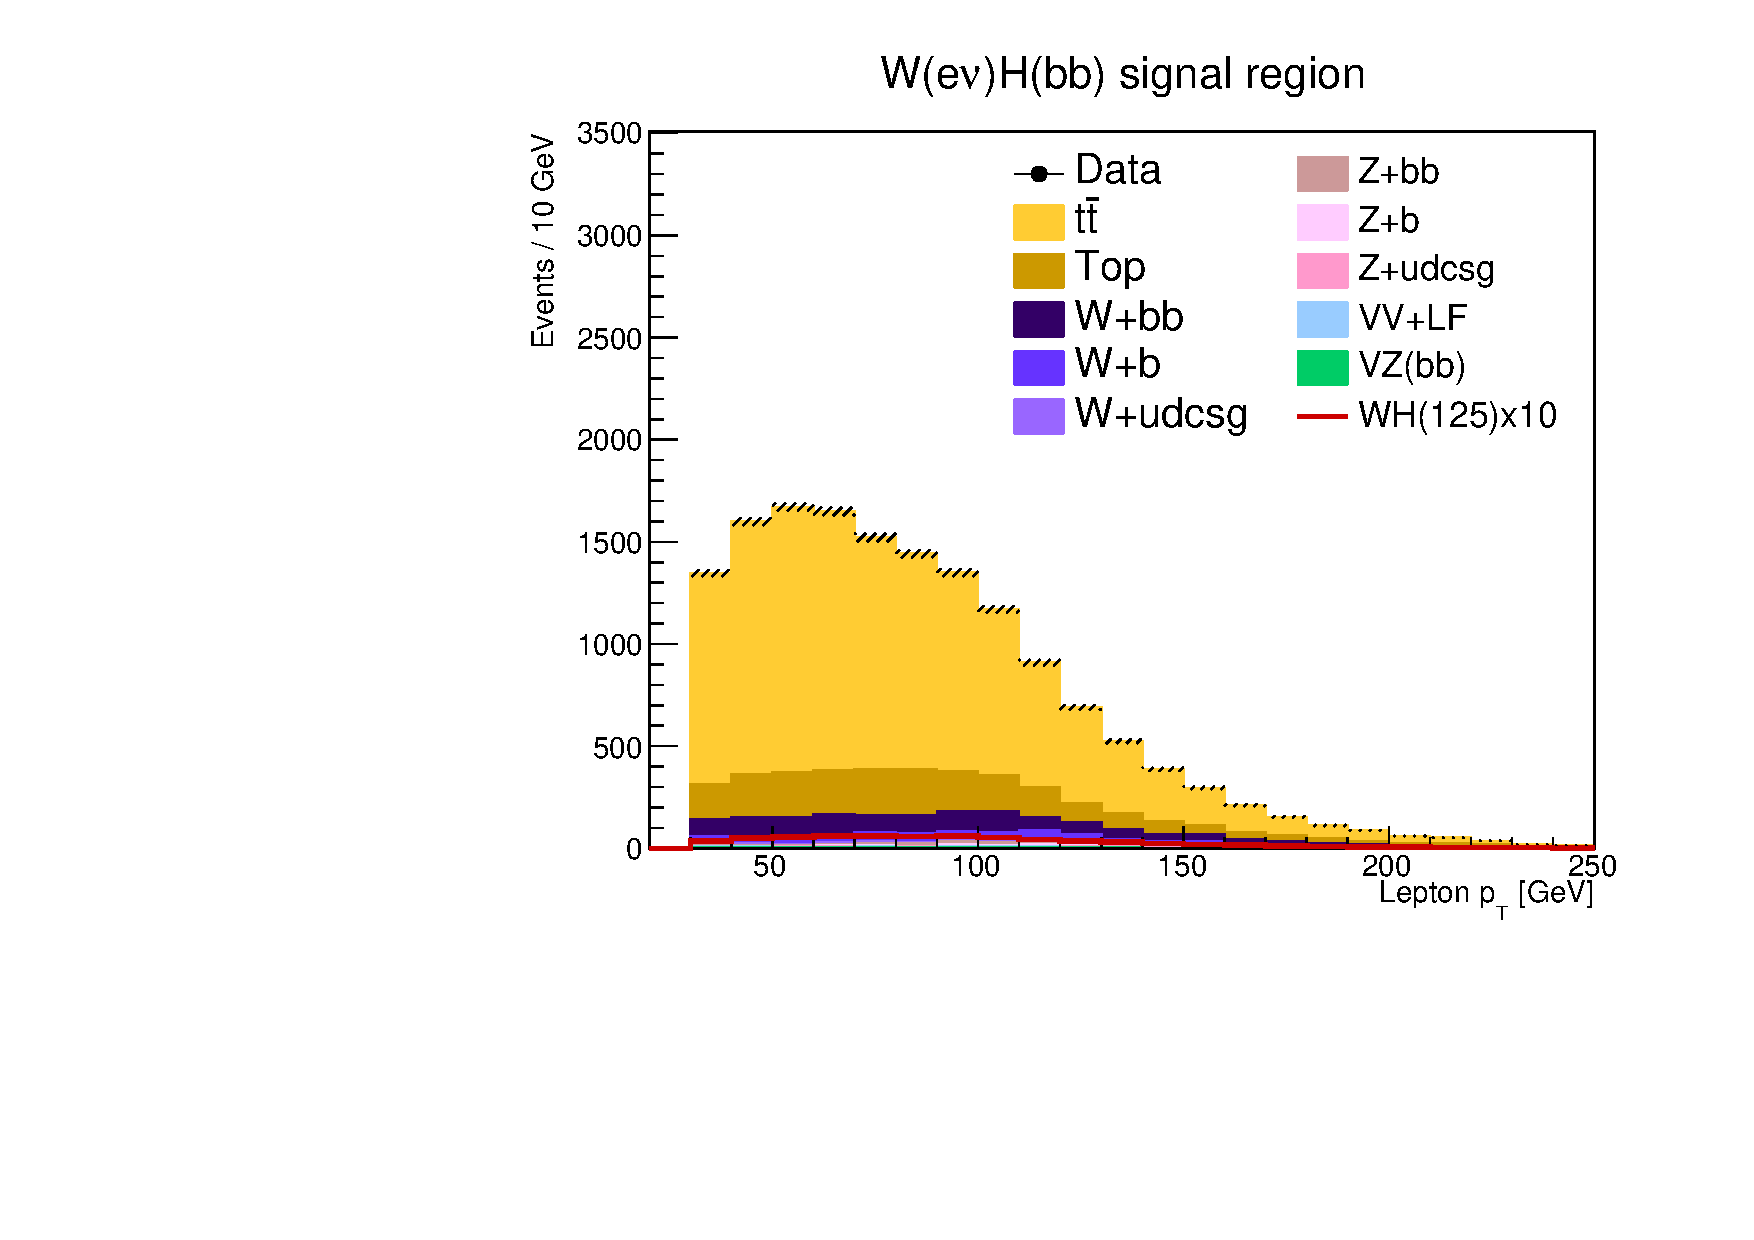
\includegraphics[width=0.48\textwidth]{figures/wlnhbb2016/resolved/WenWHSR_lepton1Pt.pdf}
    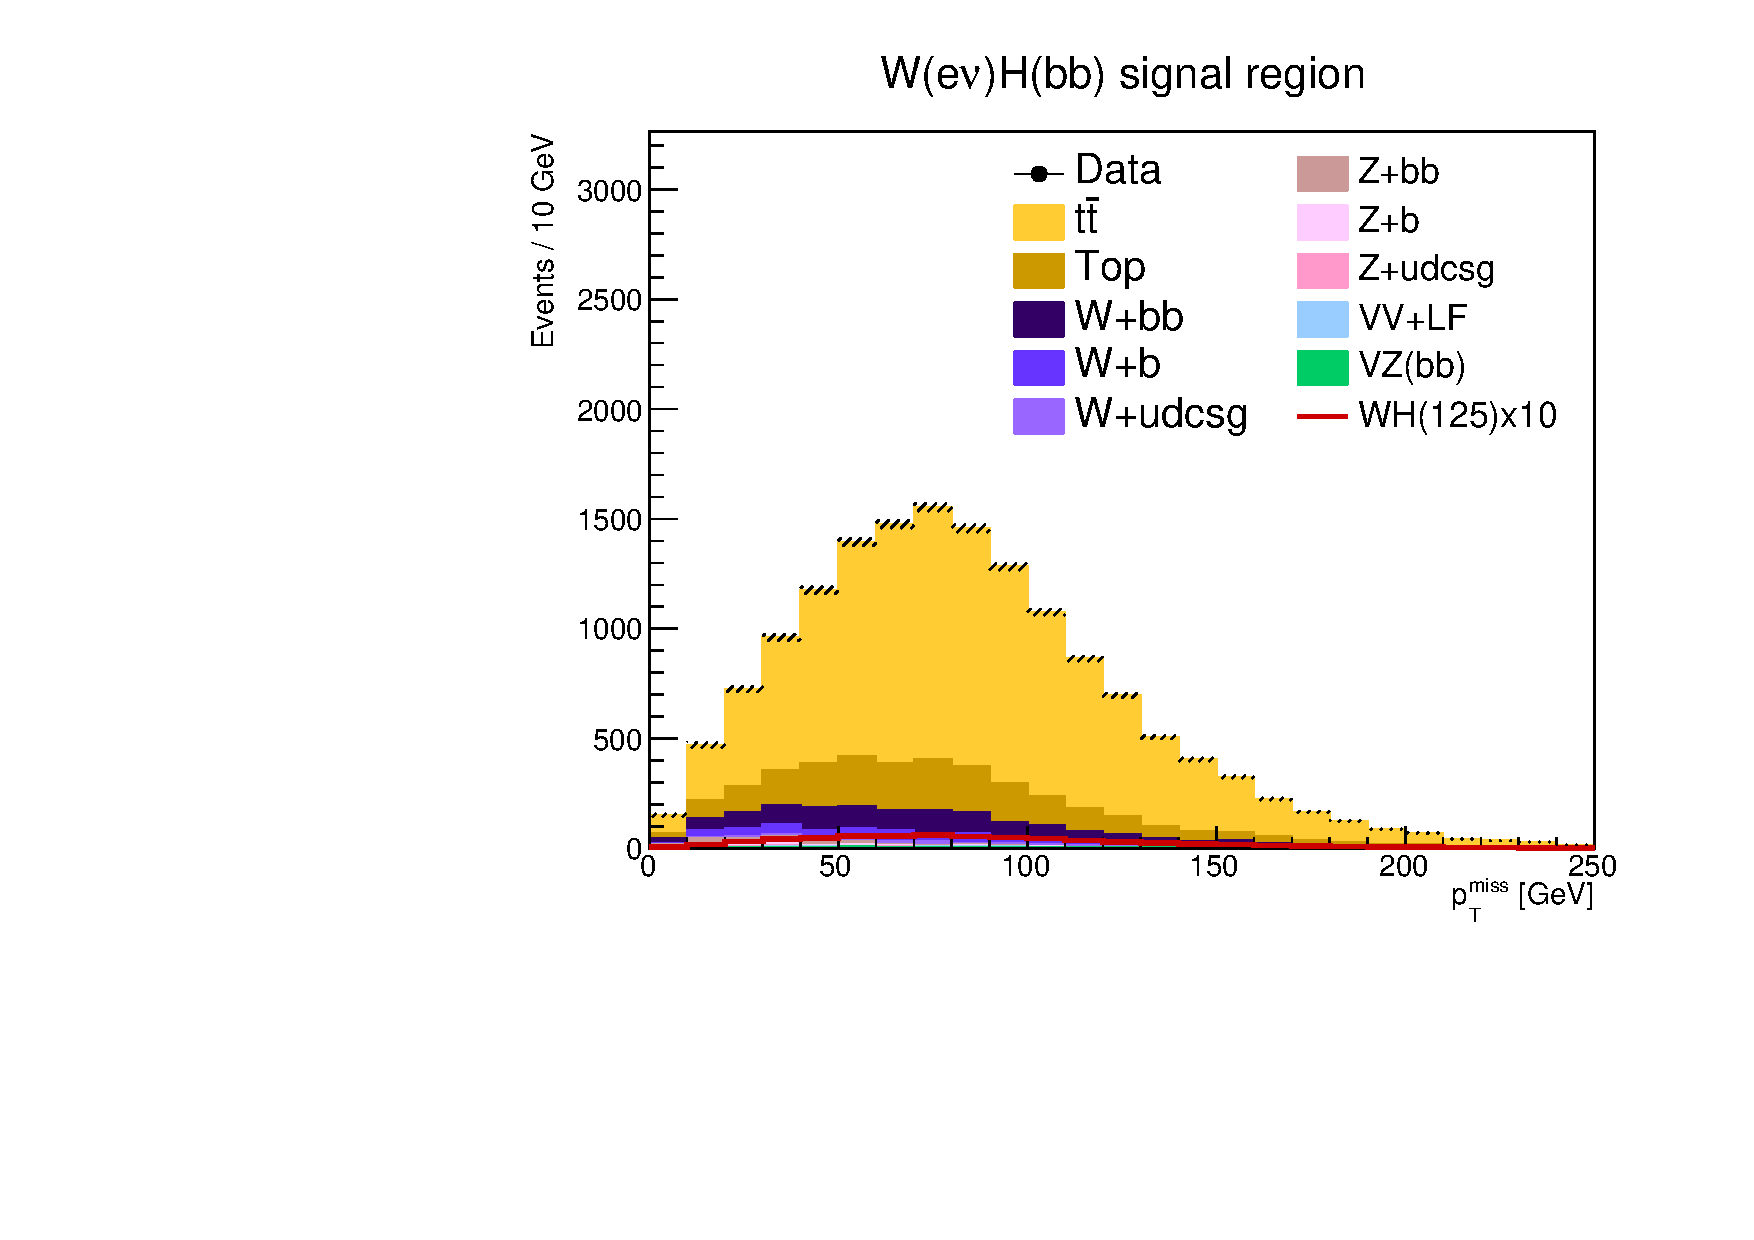
\includegraphics[width=0.48\textwidth]{figures/wlnhbb2016/resolved/WenWHSR_pfmet.pdf}
    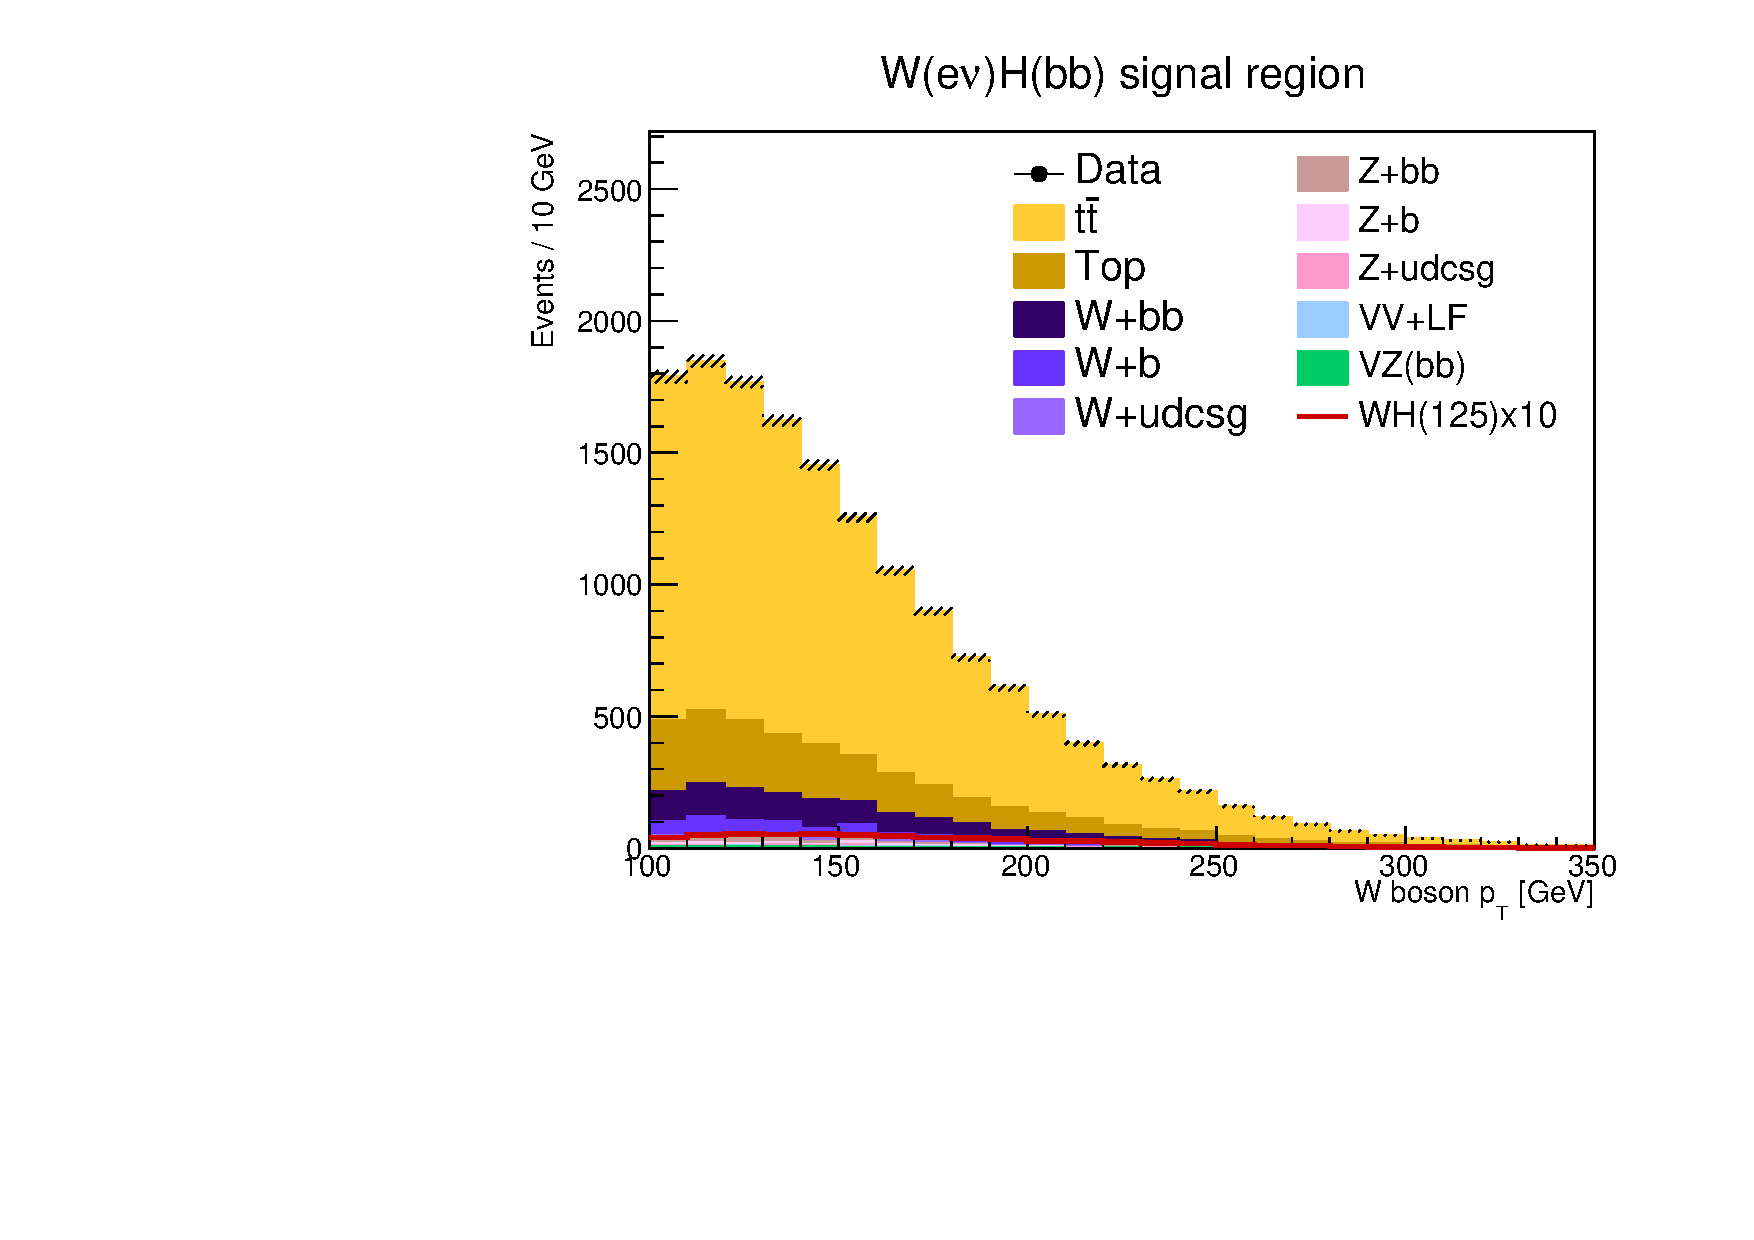
\includegraphics[width=0.48\textwidth]{figures/wlnhbb2016/resolved/WenWHSR_WpT.pdf}
    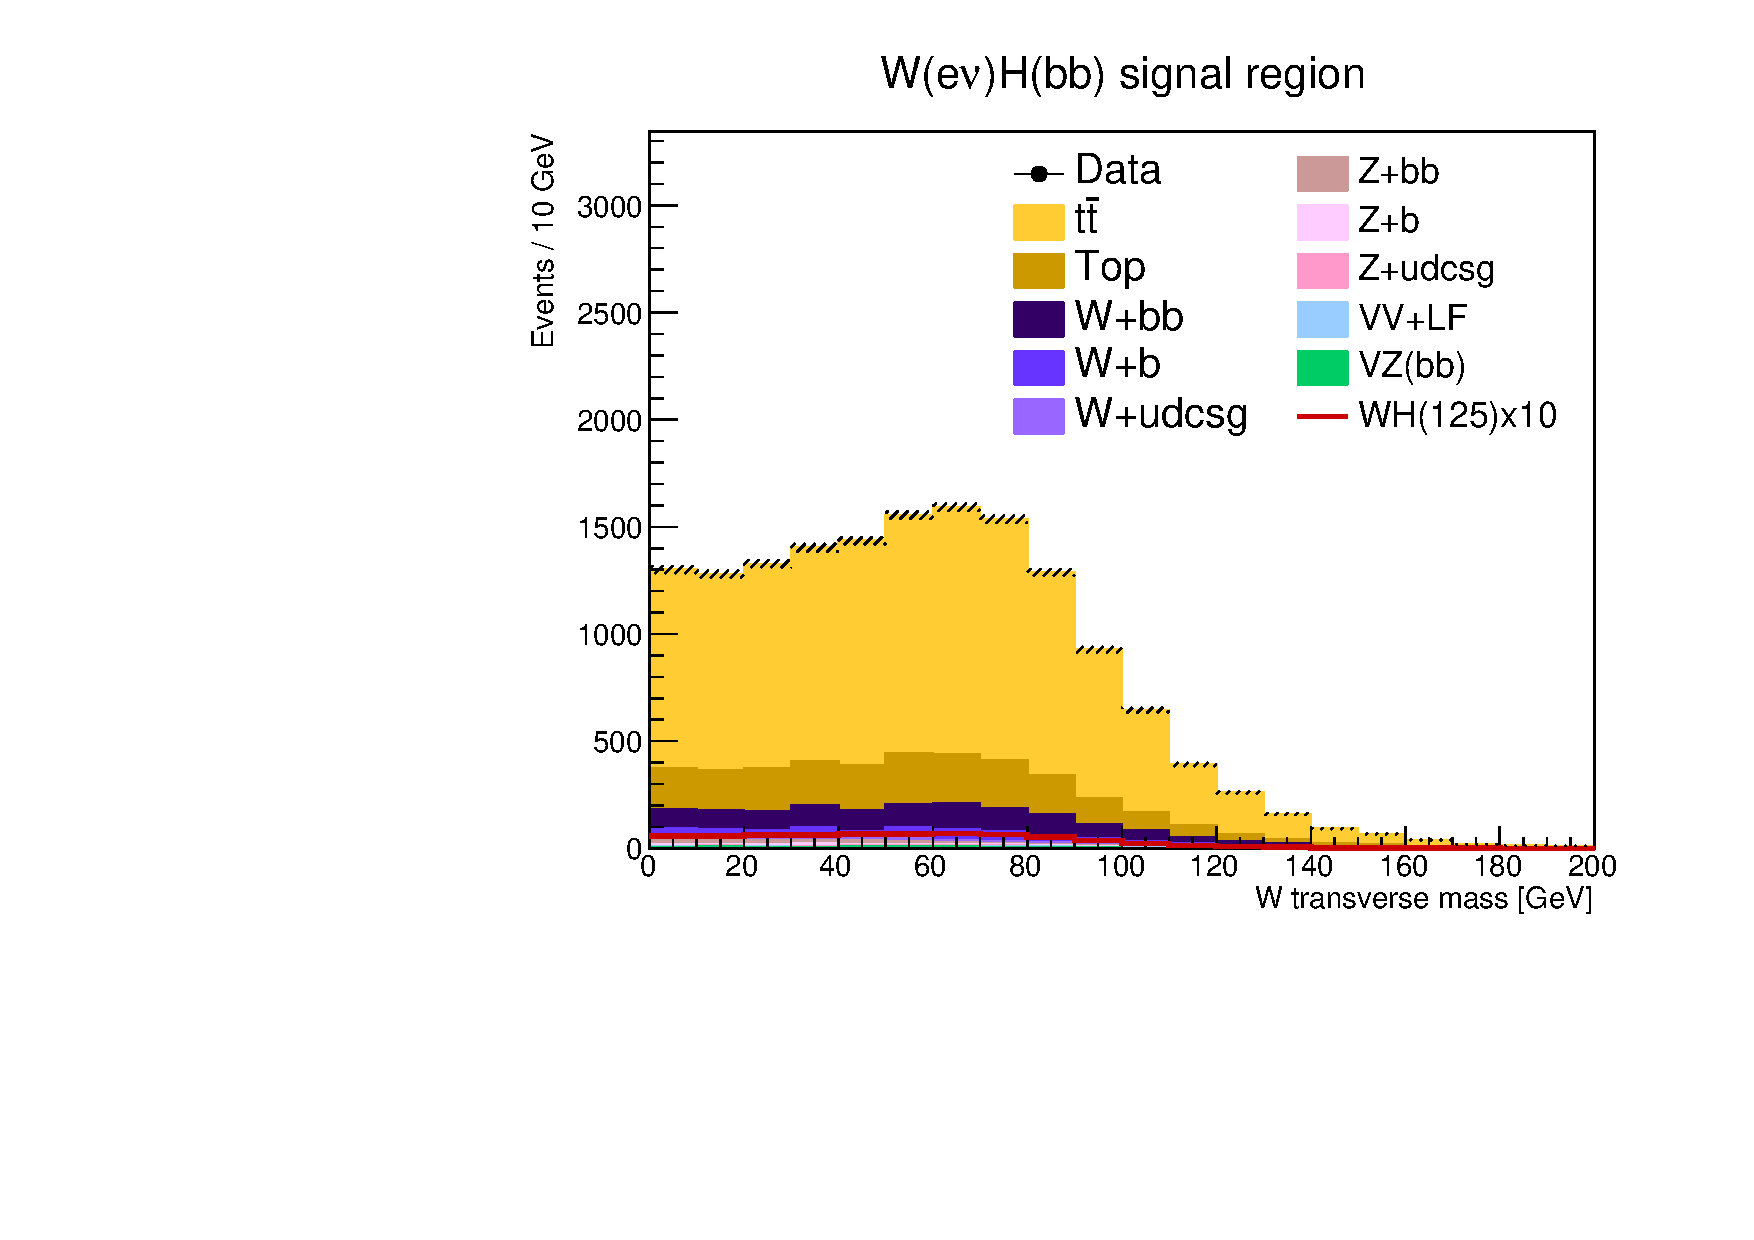
\includegraphics[width=0.48\textwidth]{figures/wlnhbb2016/resolved/WenWHSR_mTW.pdf}
    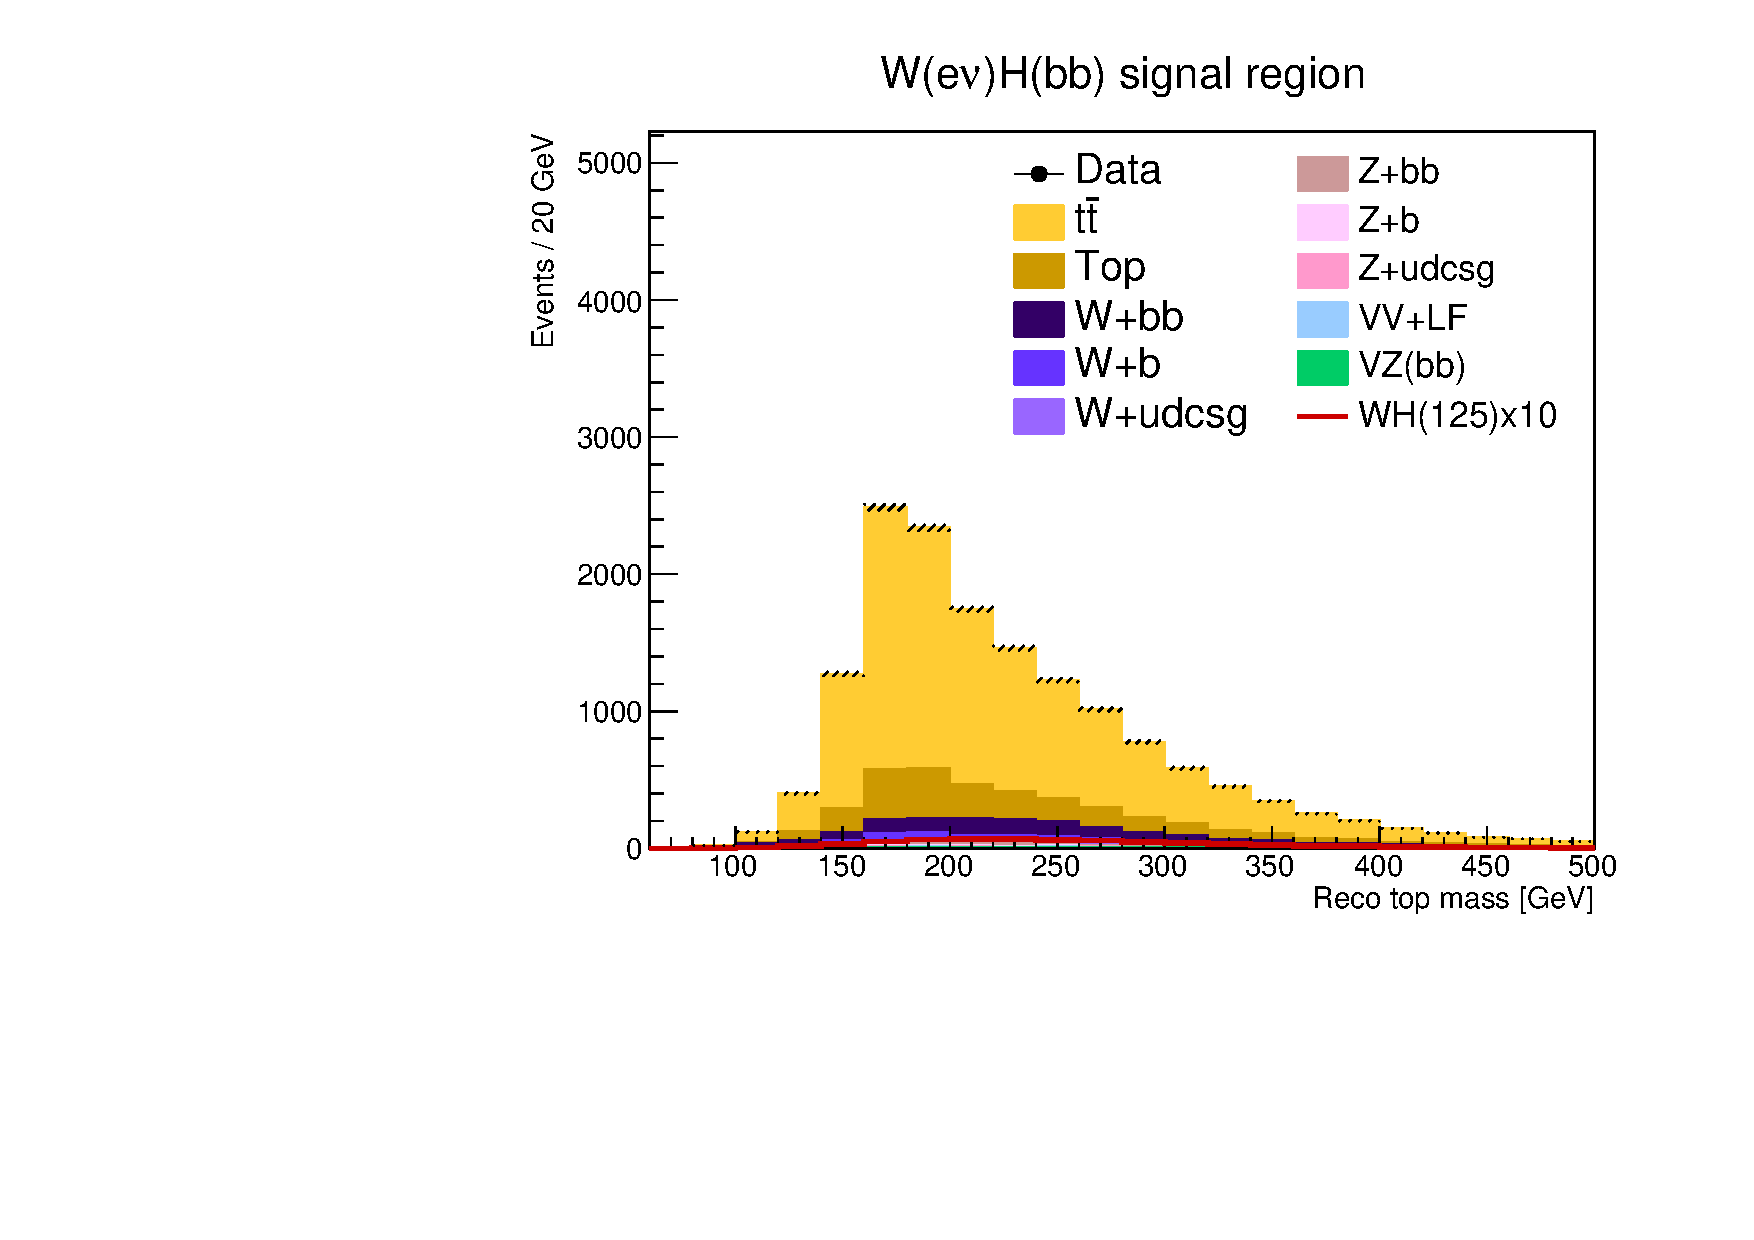
\includegraphics[width=0.48\textwidth]{figures/wlnhbb2016/resolved/WenWHSR_topMassLep1Met.pdf}
    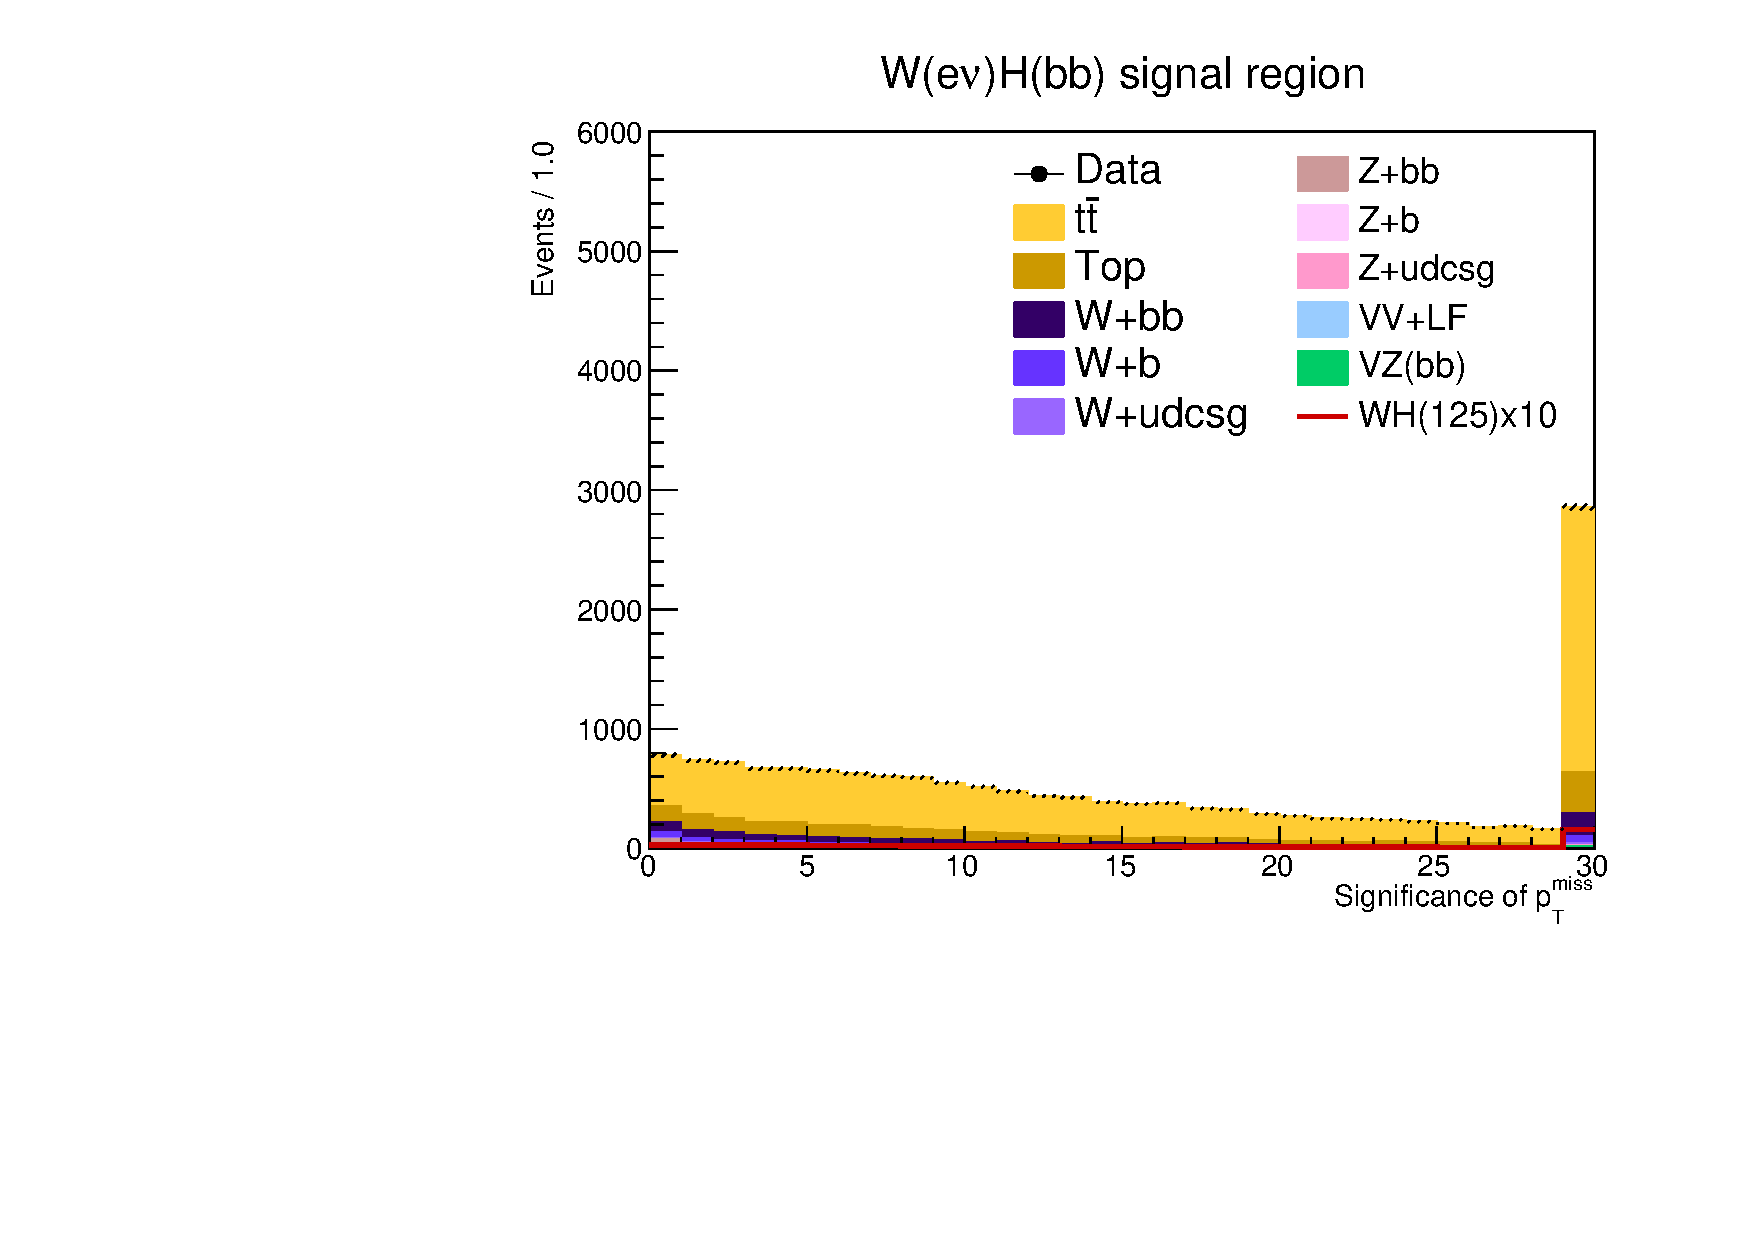
\includegraphics[width=0.48\textwidth]{figures/wlnhbb2016/resolved/WenWHSR_pfmetsig.pdf}
    \caption{W boson reconstruction in the resolved category W(e$\nu$) signal region.
    Left to right and top to bottom: electron $\pt$, $\MET$, W boson $\pt$, W boson transverse mass,
    the reconstructed top quark mass, and the $\MET$ significance.
    The simulated shapes are prefit, with the postfit normalizations applied.}
    \label{fig:res_WenSR_WBosons}
  \end{center}
\end{figure}
\clearpage

\begin{figure}[tbp]
  \begin{center}
    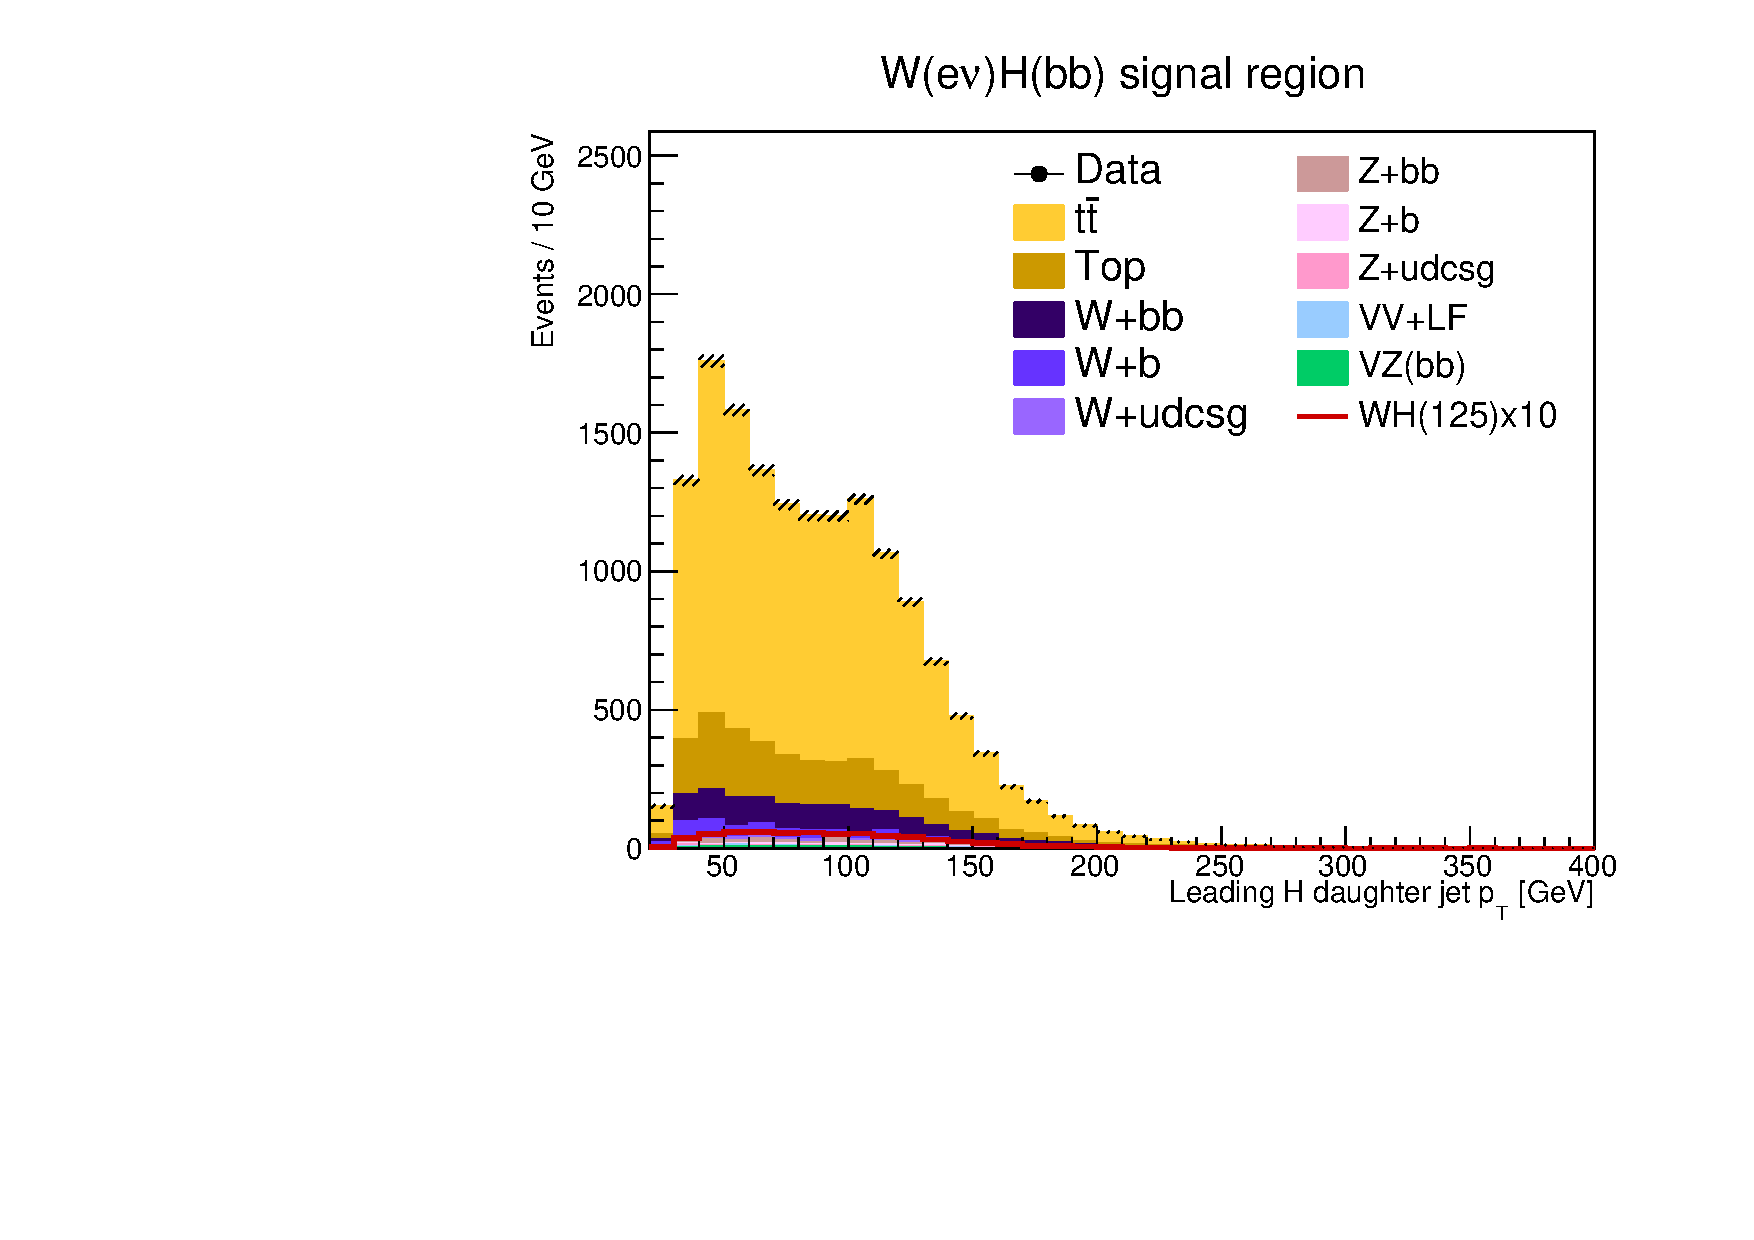
\includegraphics[width=0.48\textwidth]{figures/wlnhbb2016/resolved/WenWHSR_Hbjet1Pt.pdf}
    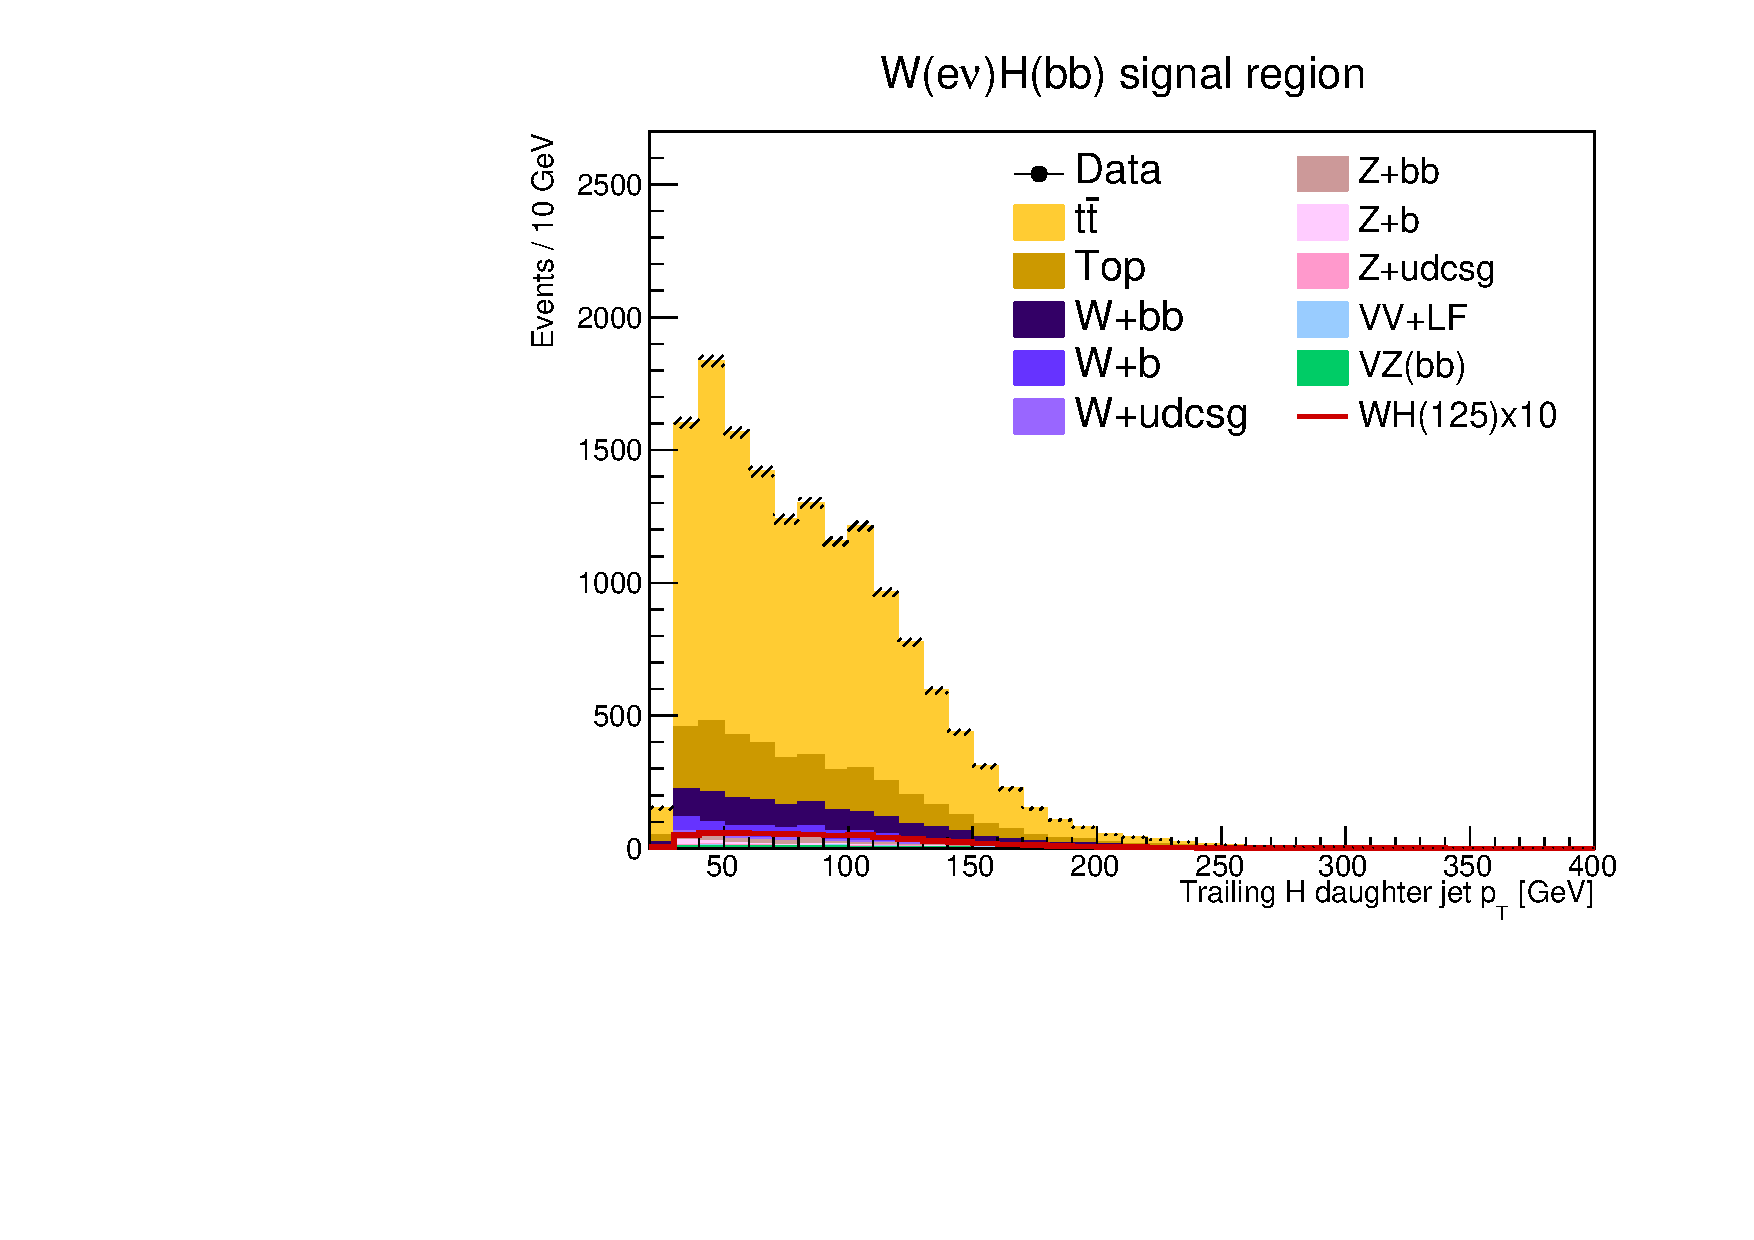
\includegraphics[width=0.48\textwidth]{figures/wlnhbb2016/resolved/WenWHSR_Hbjet2Pt.pdf}
    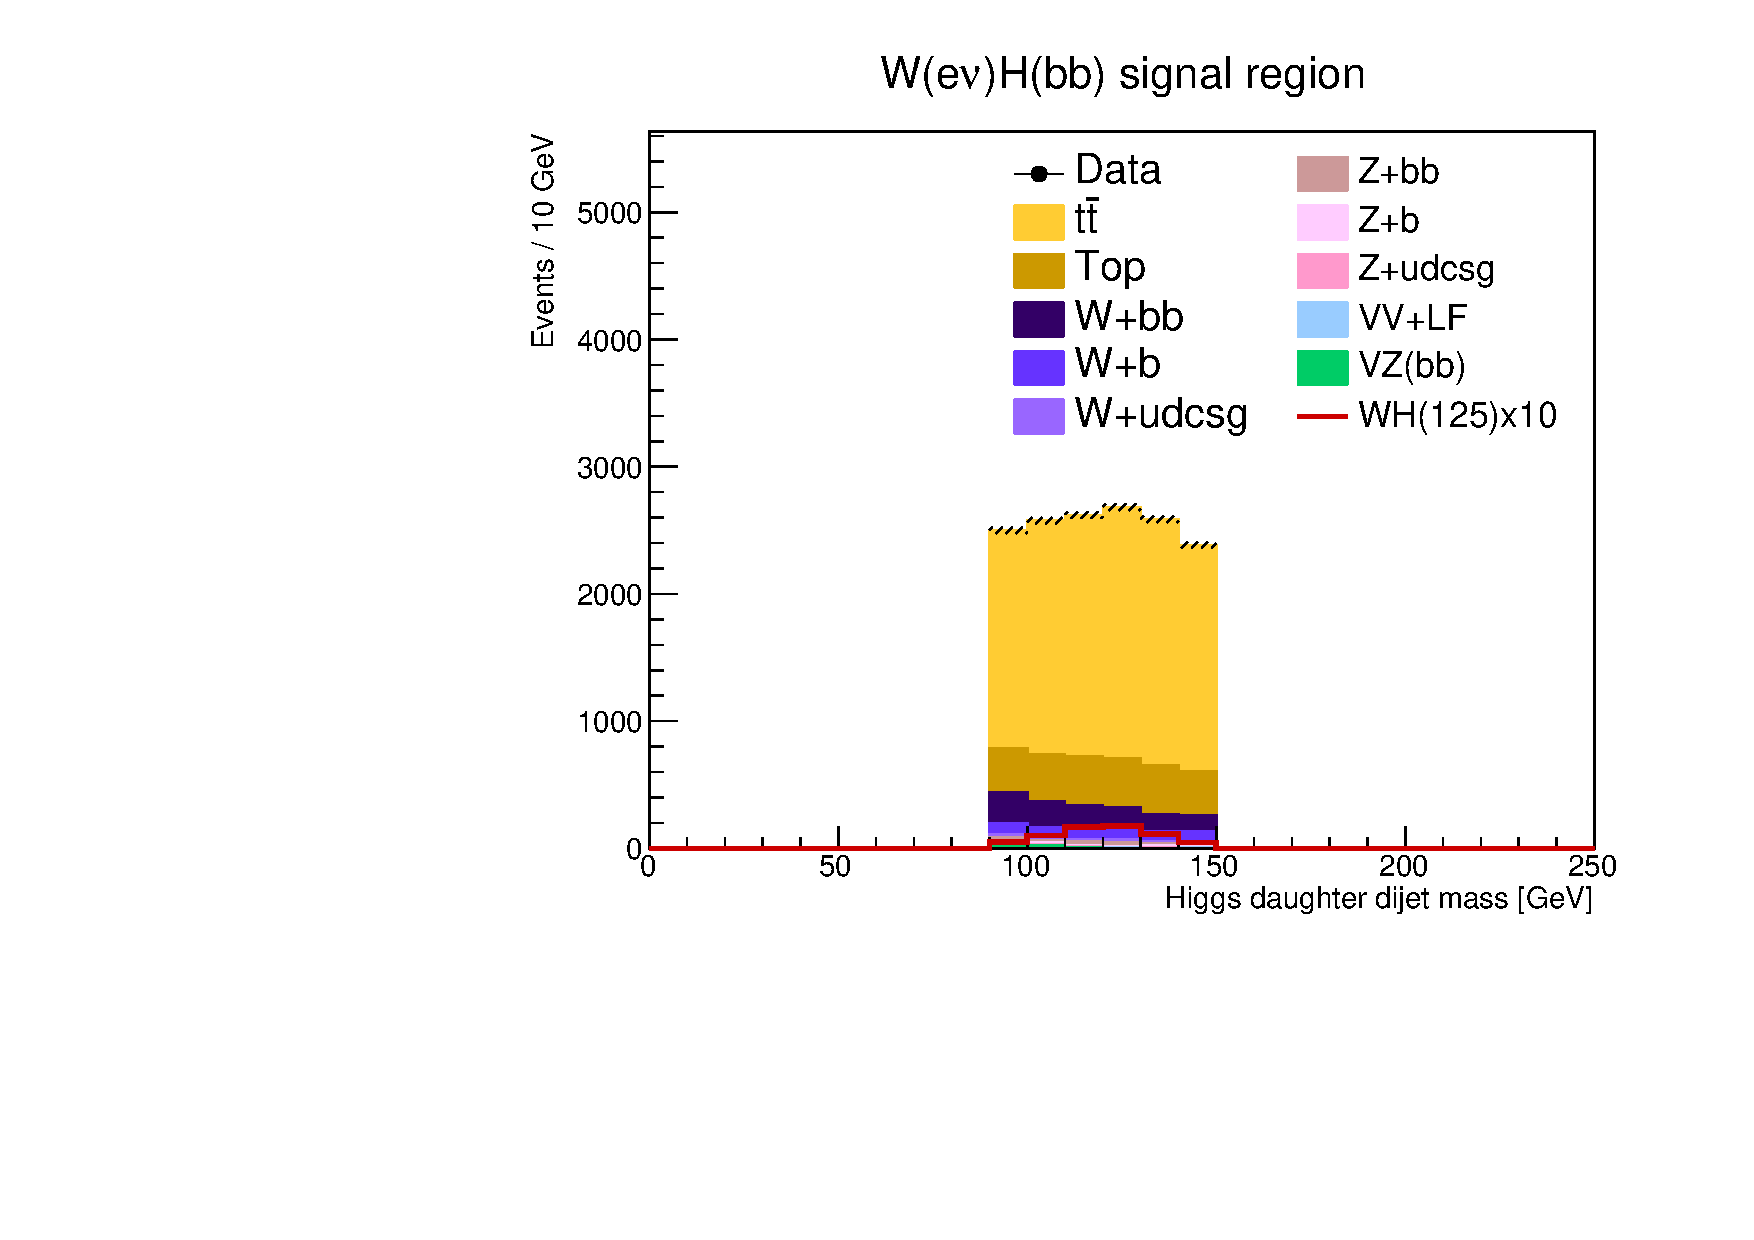
\includegraphics[width=0.48\textwidth]{figures/wlnhbb2016/resolved/WenWHSR_mH.pdf}
    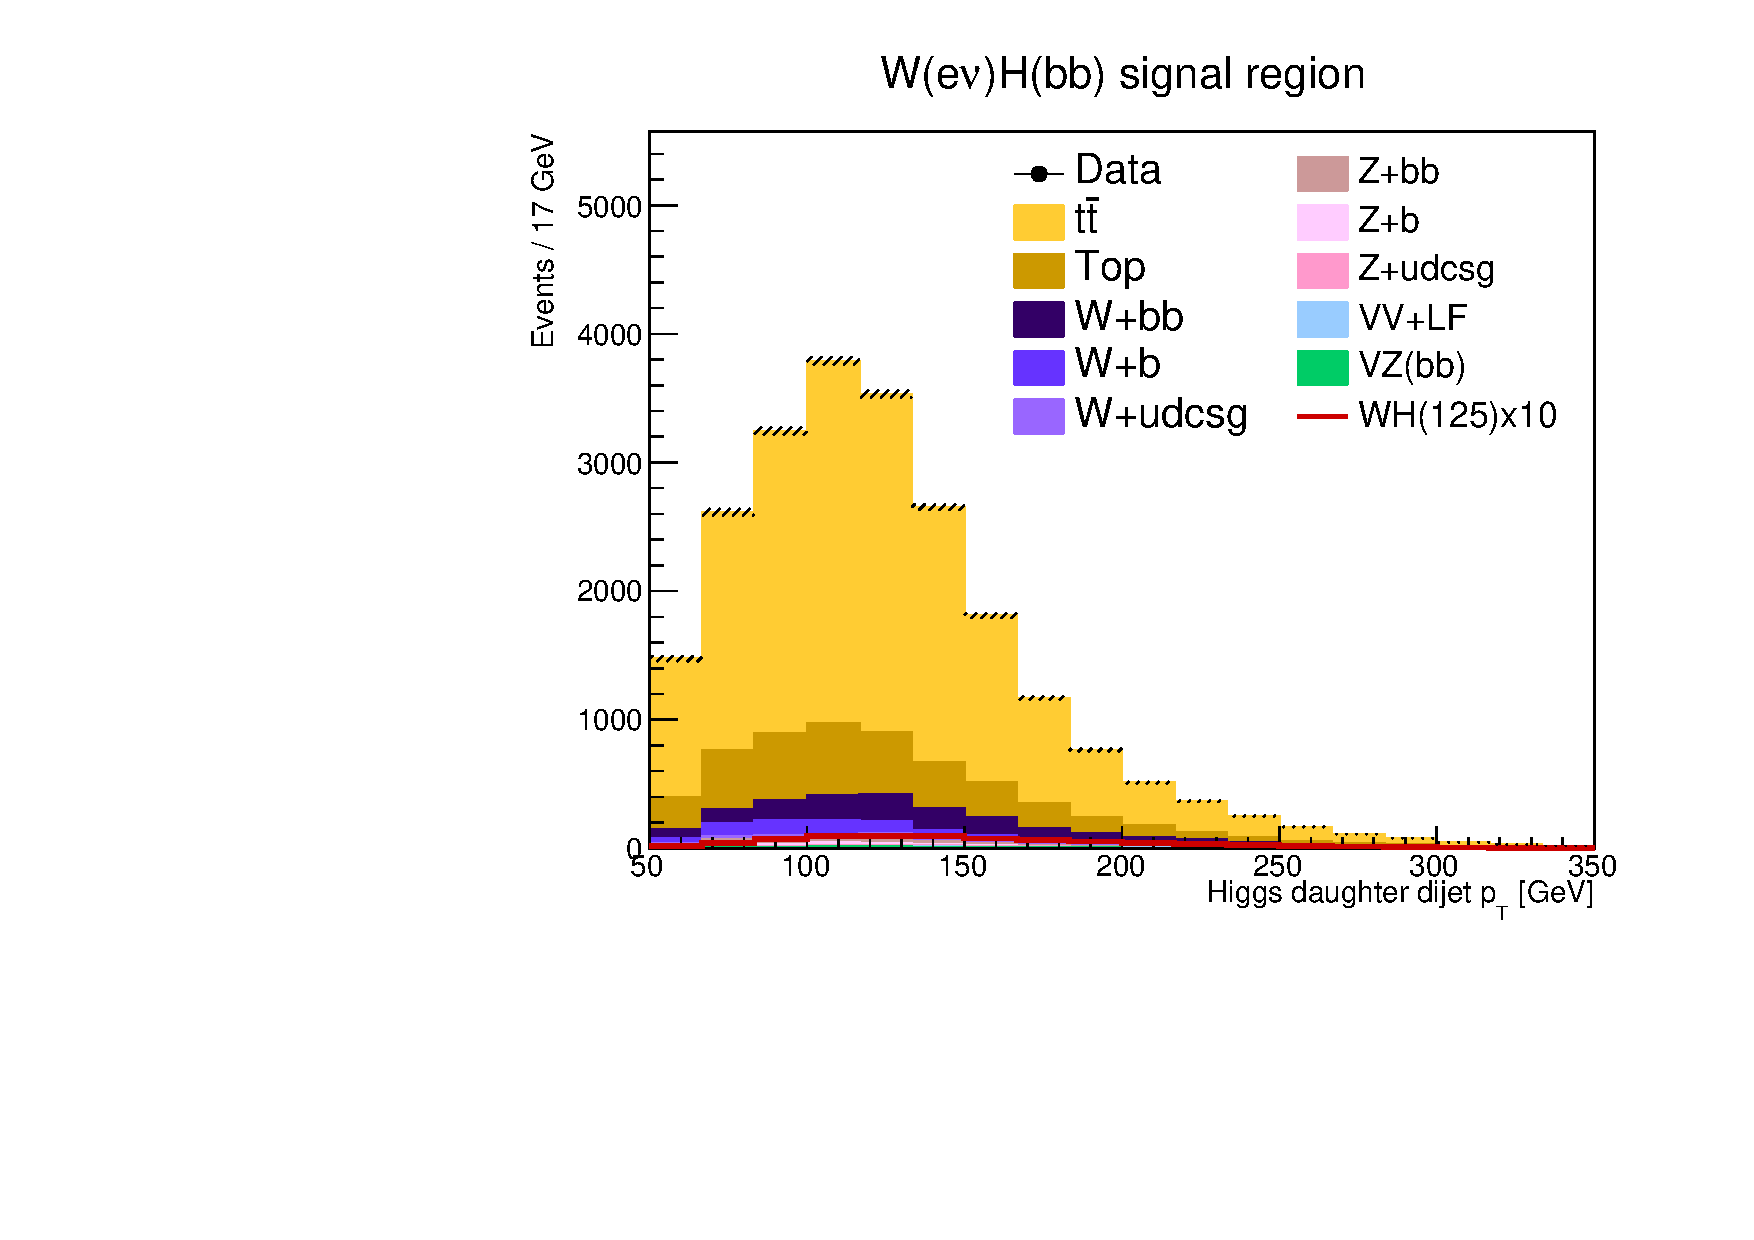
\includegraphics[width=0.48\textwidth]{figures/wlnhbb2016/resolved/WenWHSR_pTH.pdf}
    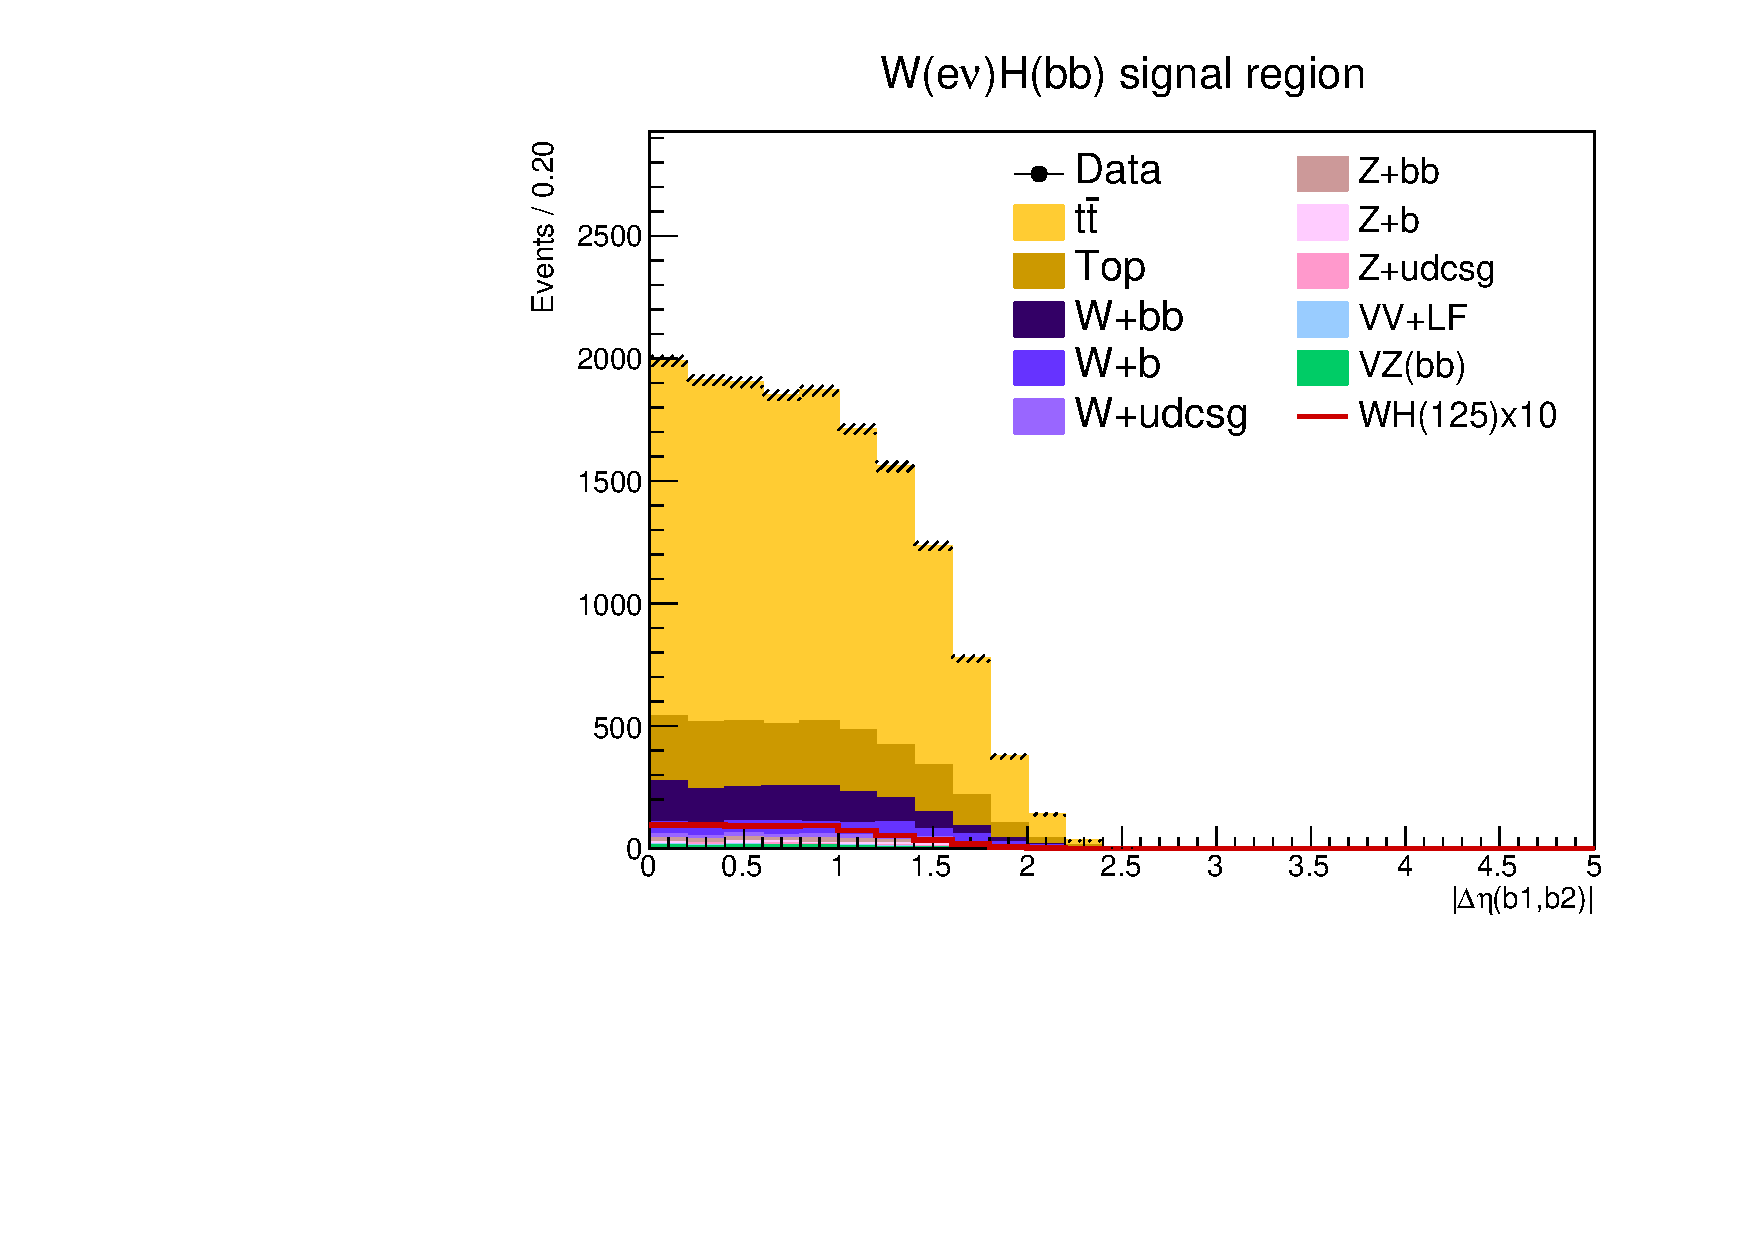
\includegraphics[width=0.48\textwidth]{figures/wlnhbb2016/resolved/WenWHSR_dEtab1b2.pdf}
    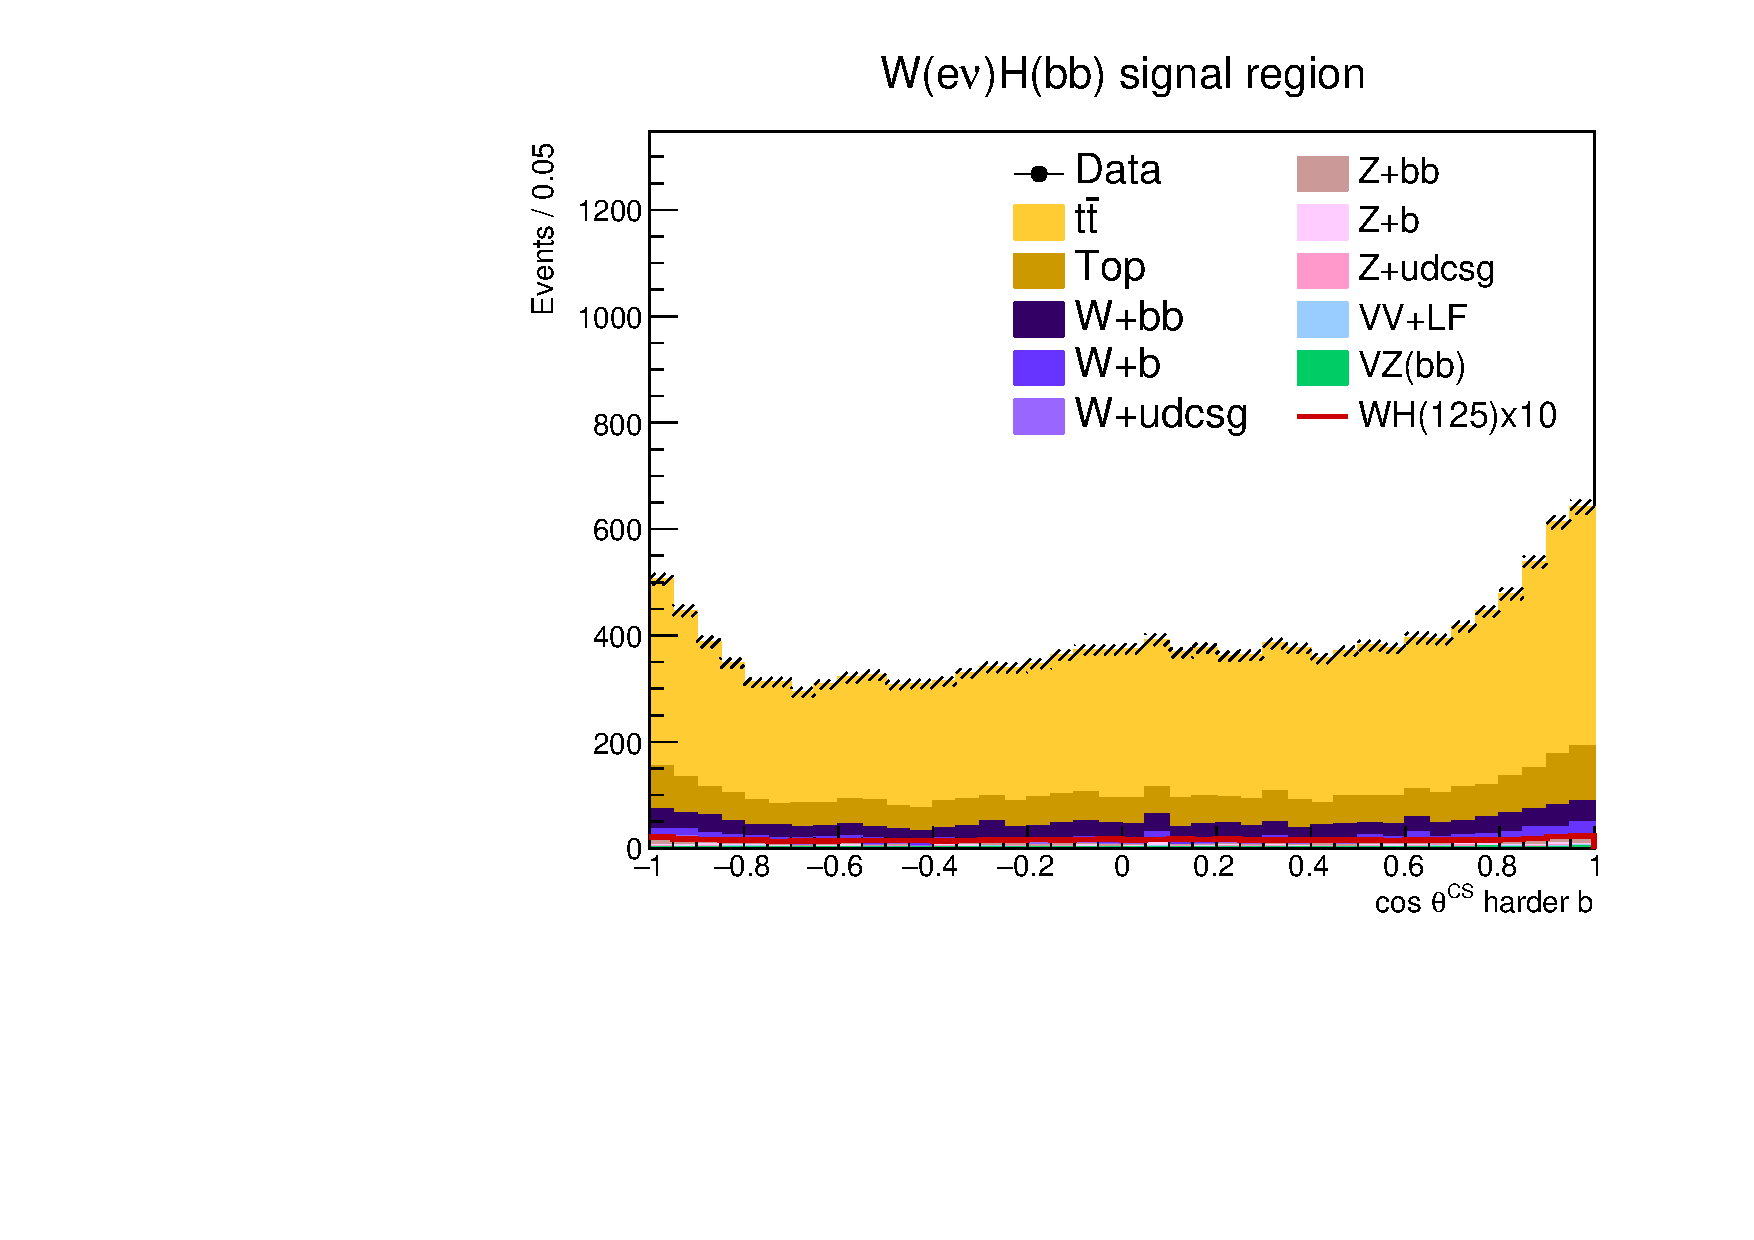
\includegraphics[width=0.48\textwidth]{figures/wlnhbb2016/resolved/WenWHSR_hbbCosThetaCSJ1.pdf}
    \caption{\HBB\ reconstruction in the resolved category W(e$\nu$) signal region.
    Left to right and top to bottom: higher b-tagged jet $\pt$, lower b-tagged jet $\pt$, dijet mass, dijet $\pt$, 
    pseudorapidity difference between the two jets, and the Collins-Soper angle of the harder b-tagged jet.
    The simulated shapes are prefit, with the postfit normalizations applied.}
    \label{fig:res_WenSR_Hbb}
  \end{center}
\end{figure}
\clearpage

\begin{figure}[tbp]
  \begin{center}
    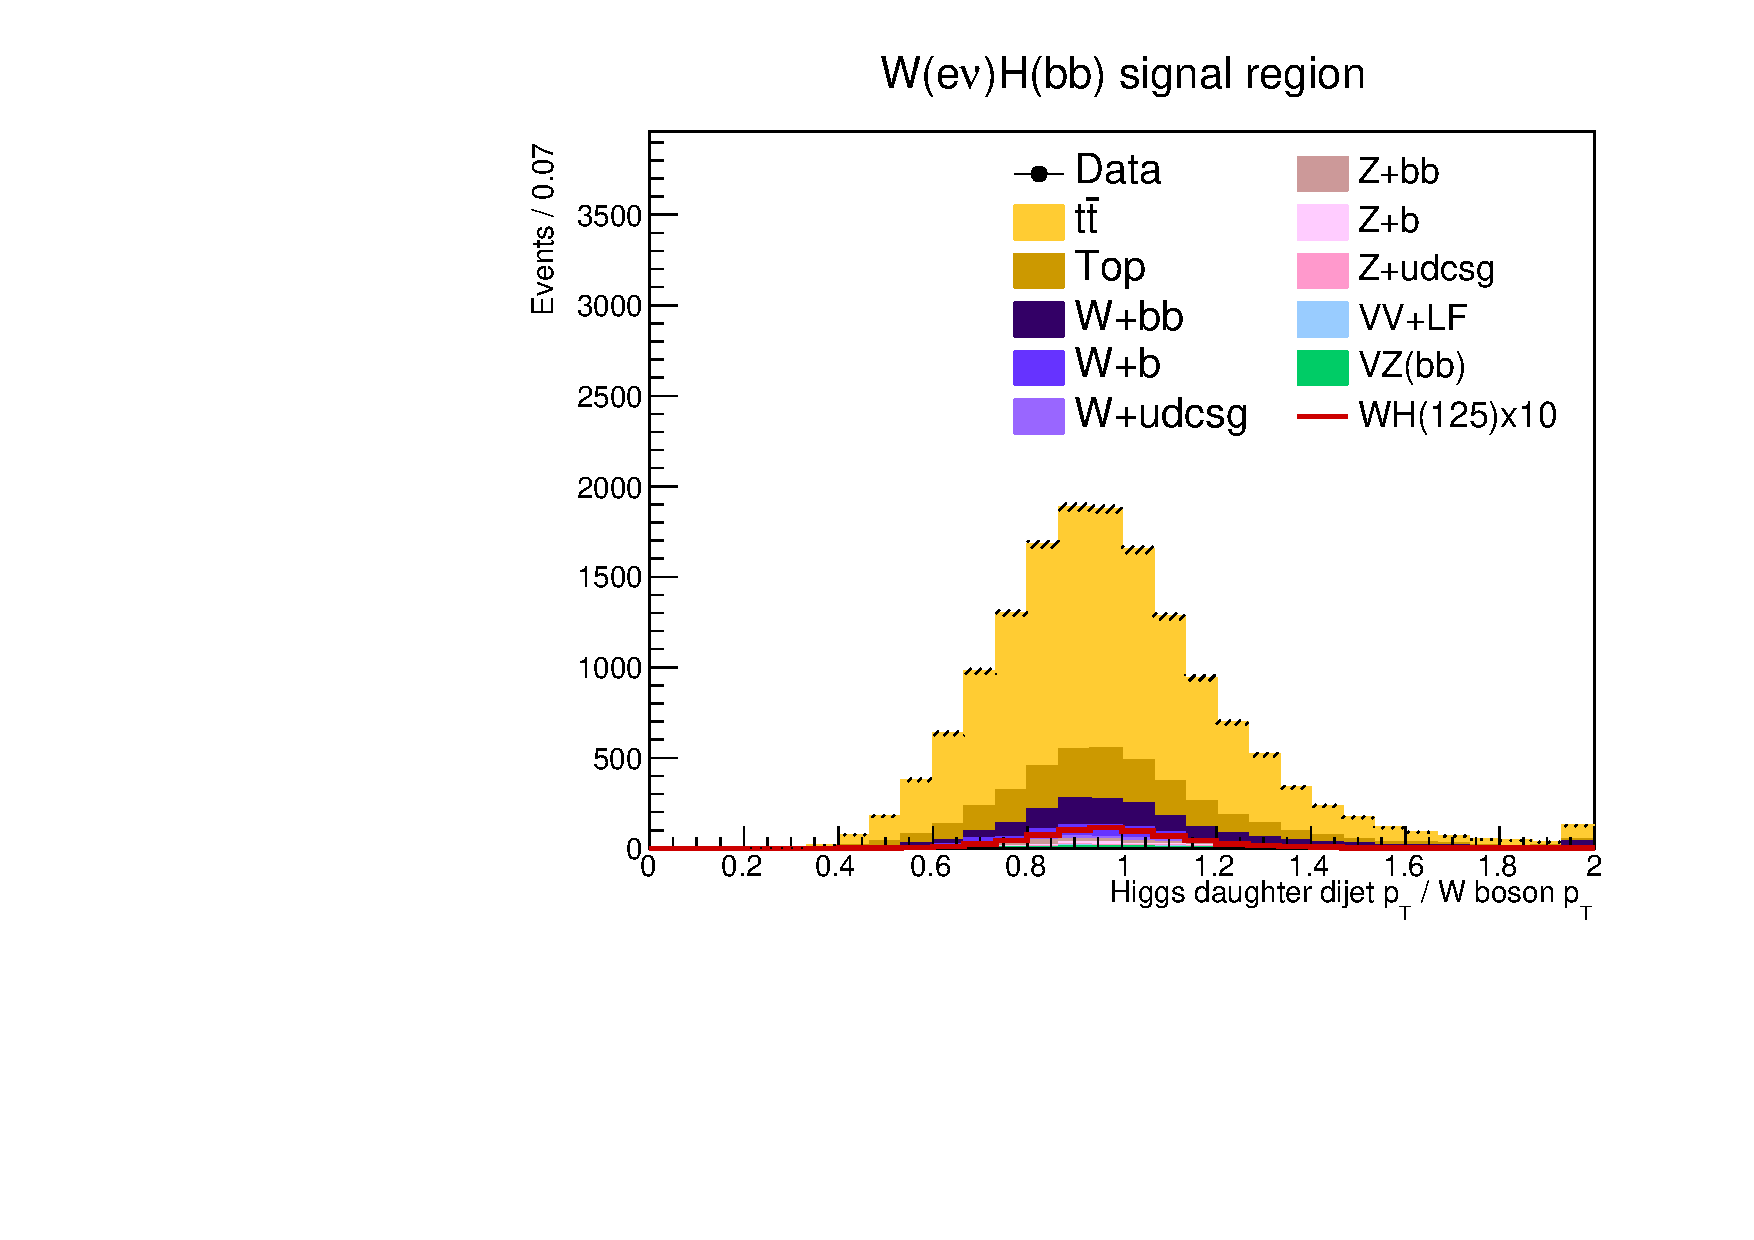
\includegraphics[width=0.48\textwidth]{figures/wlnhbb2016/resolved/WenWHSR_pTBalanceDijetW.pdf}
    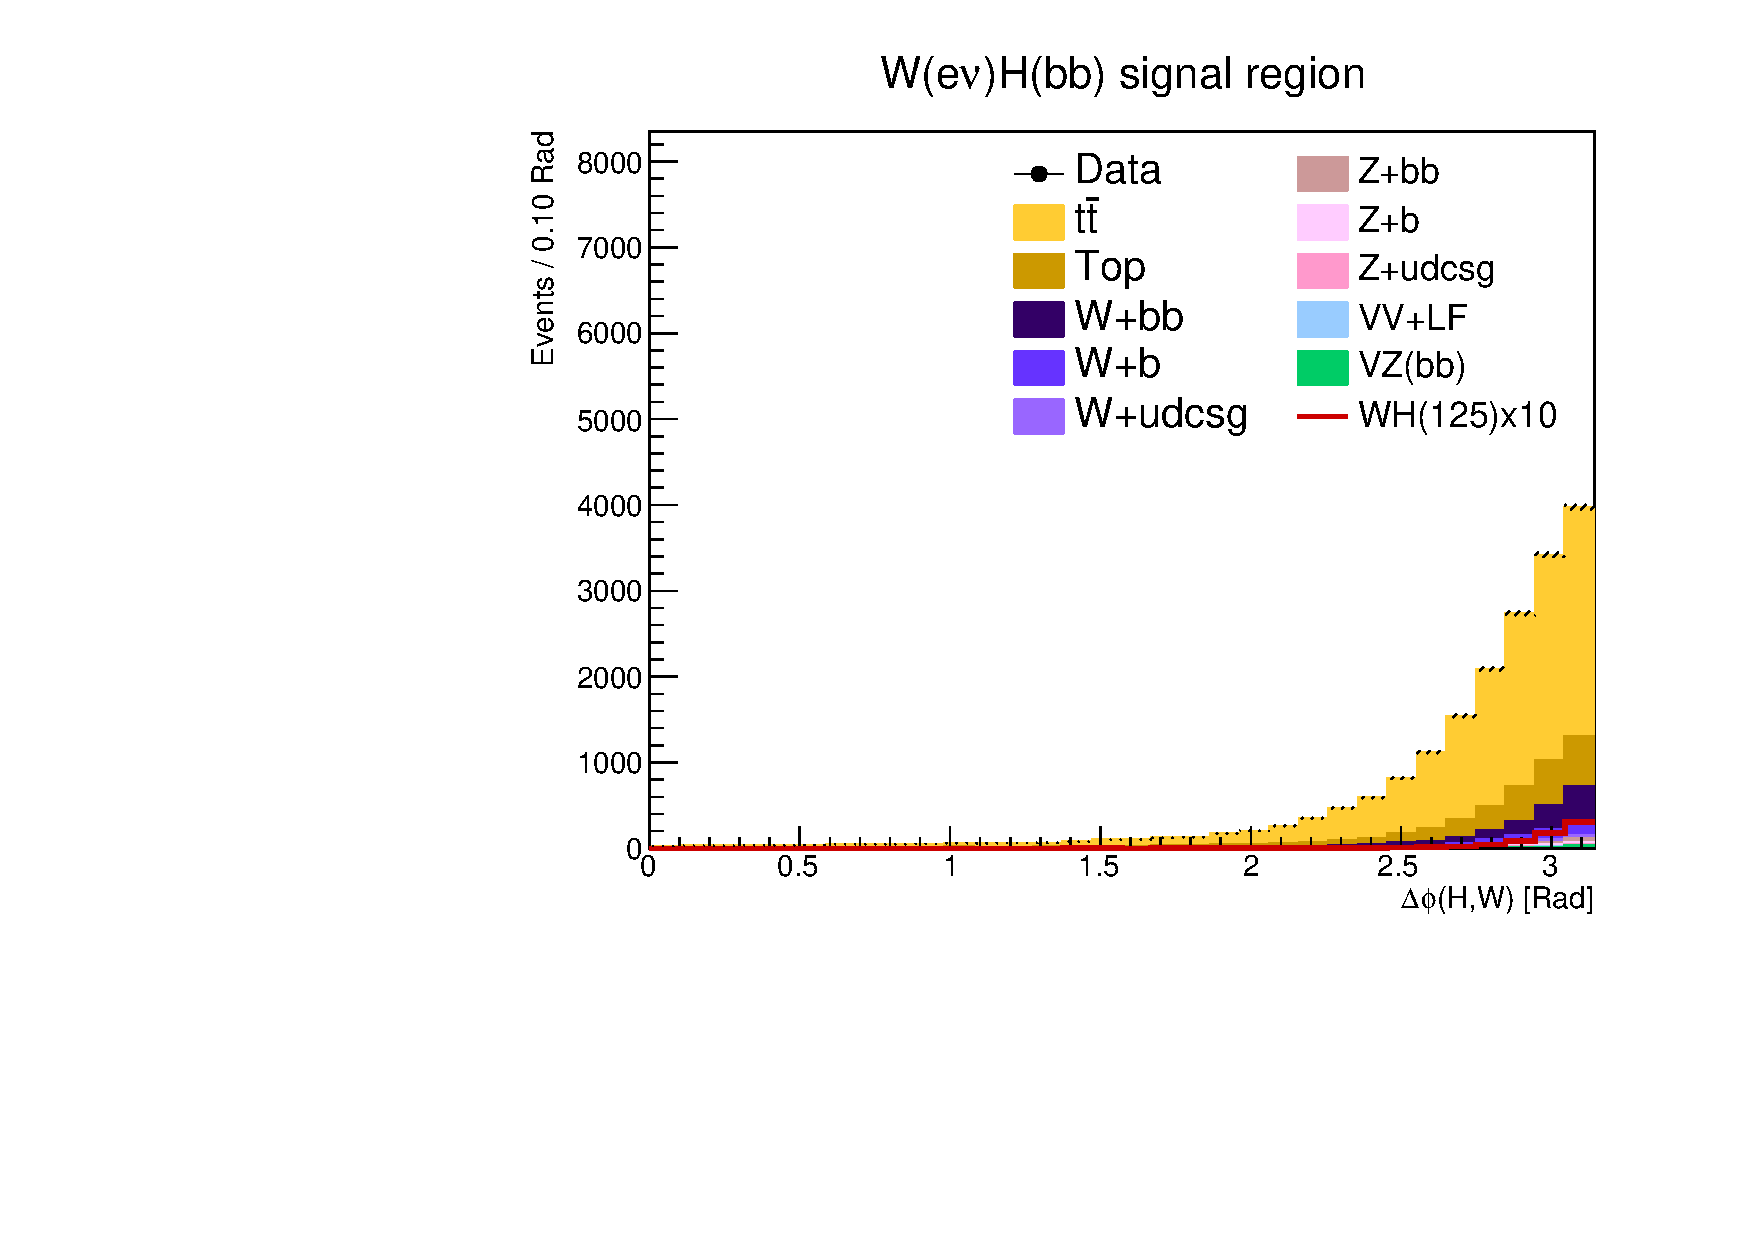
\includegraphics[width=0.48\textwidth]{figures/wlnhbb2016/resolved/WenWHSR_deltaPhiVH.pdf}
    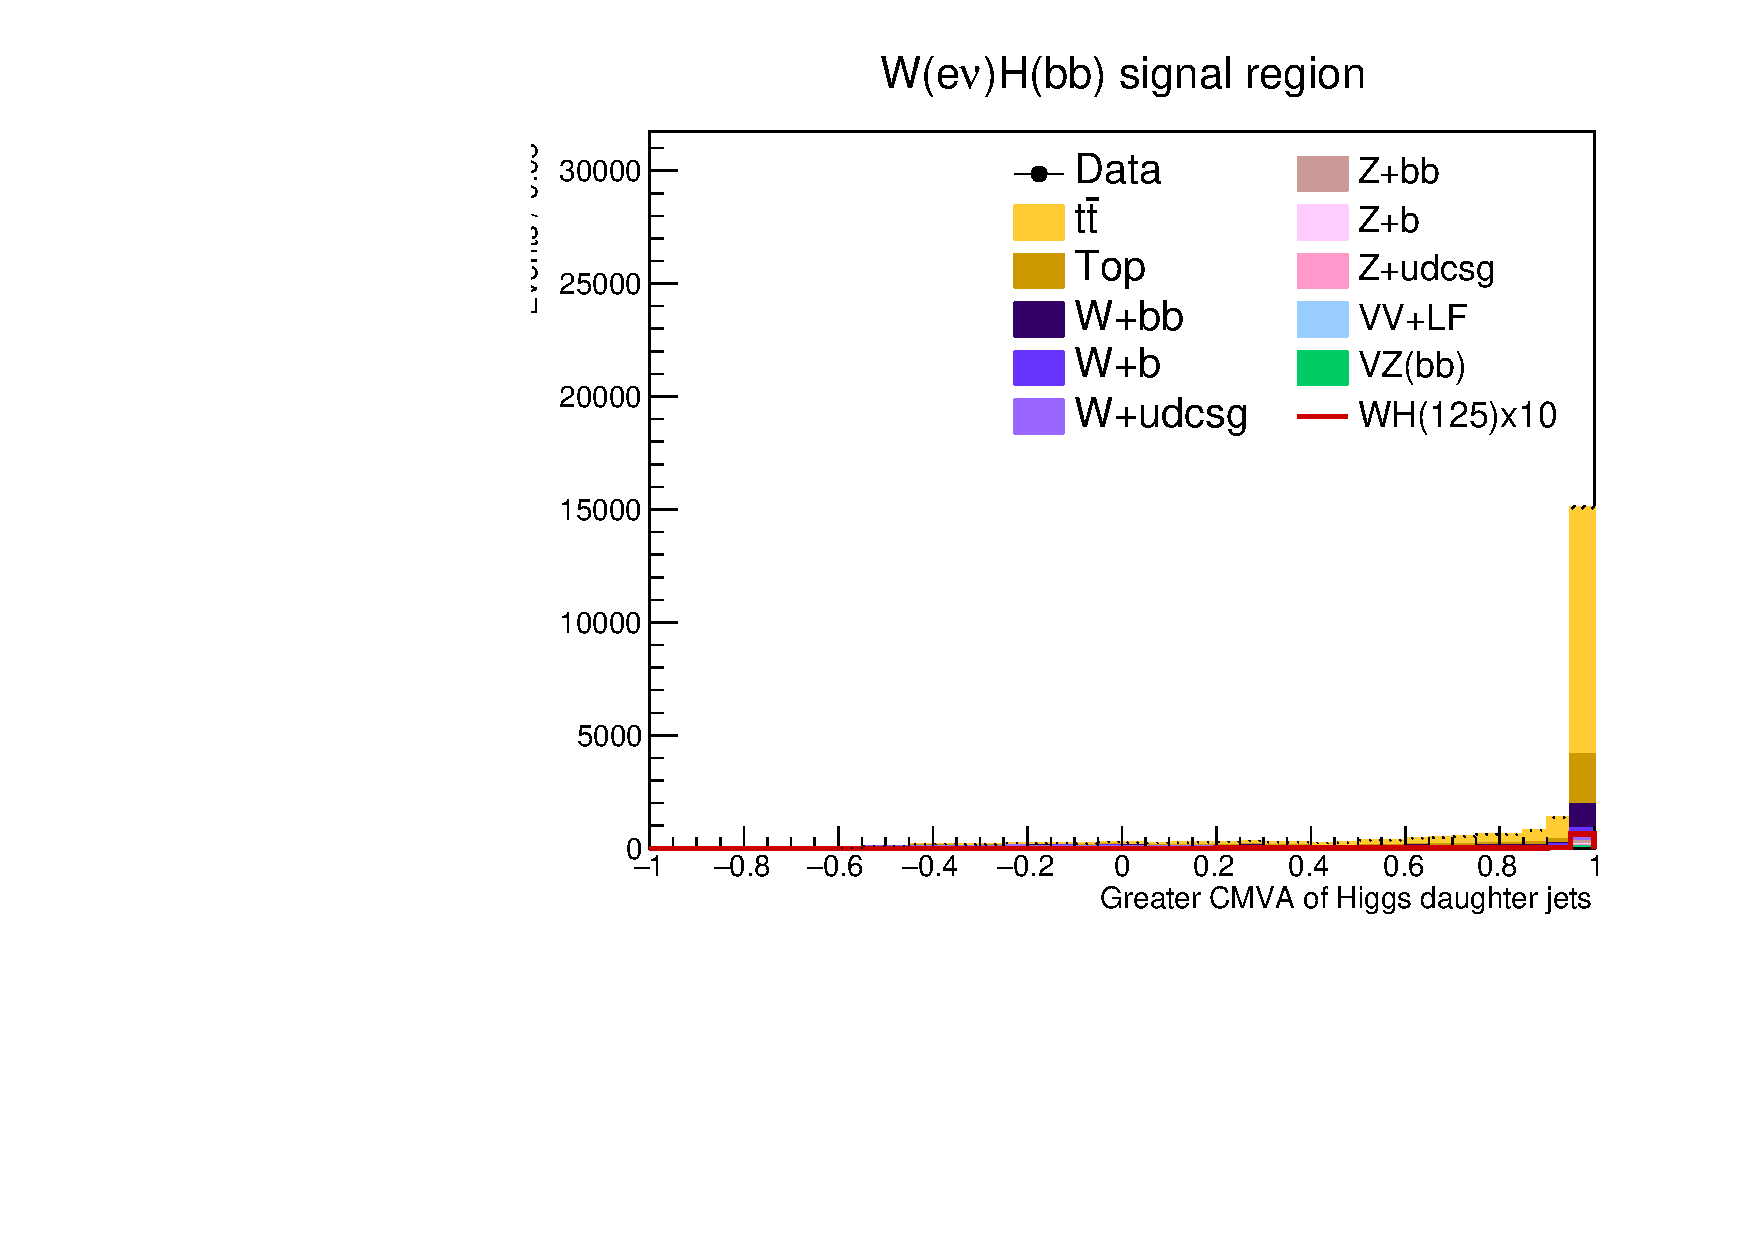
\includegraphics[width=0.48\textwidth]{figures/wlnhbb2016/resolved/WenWHSR_bDiscrMax.pdf}
    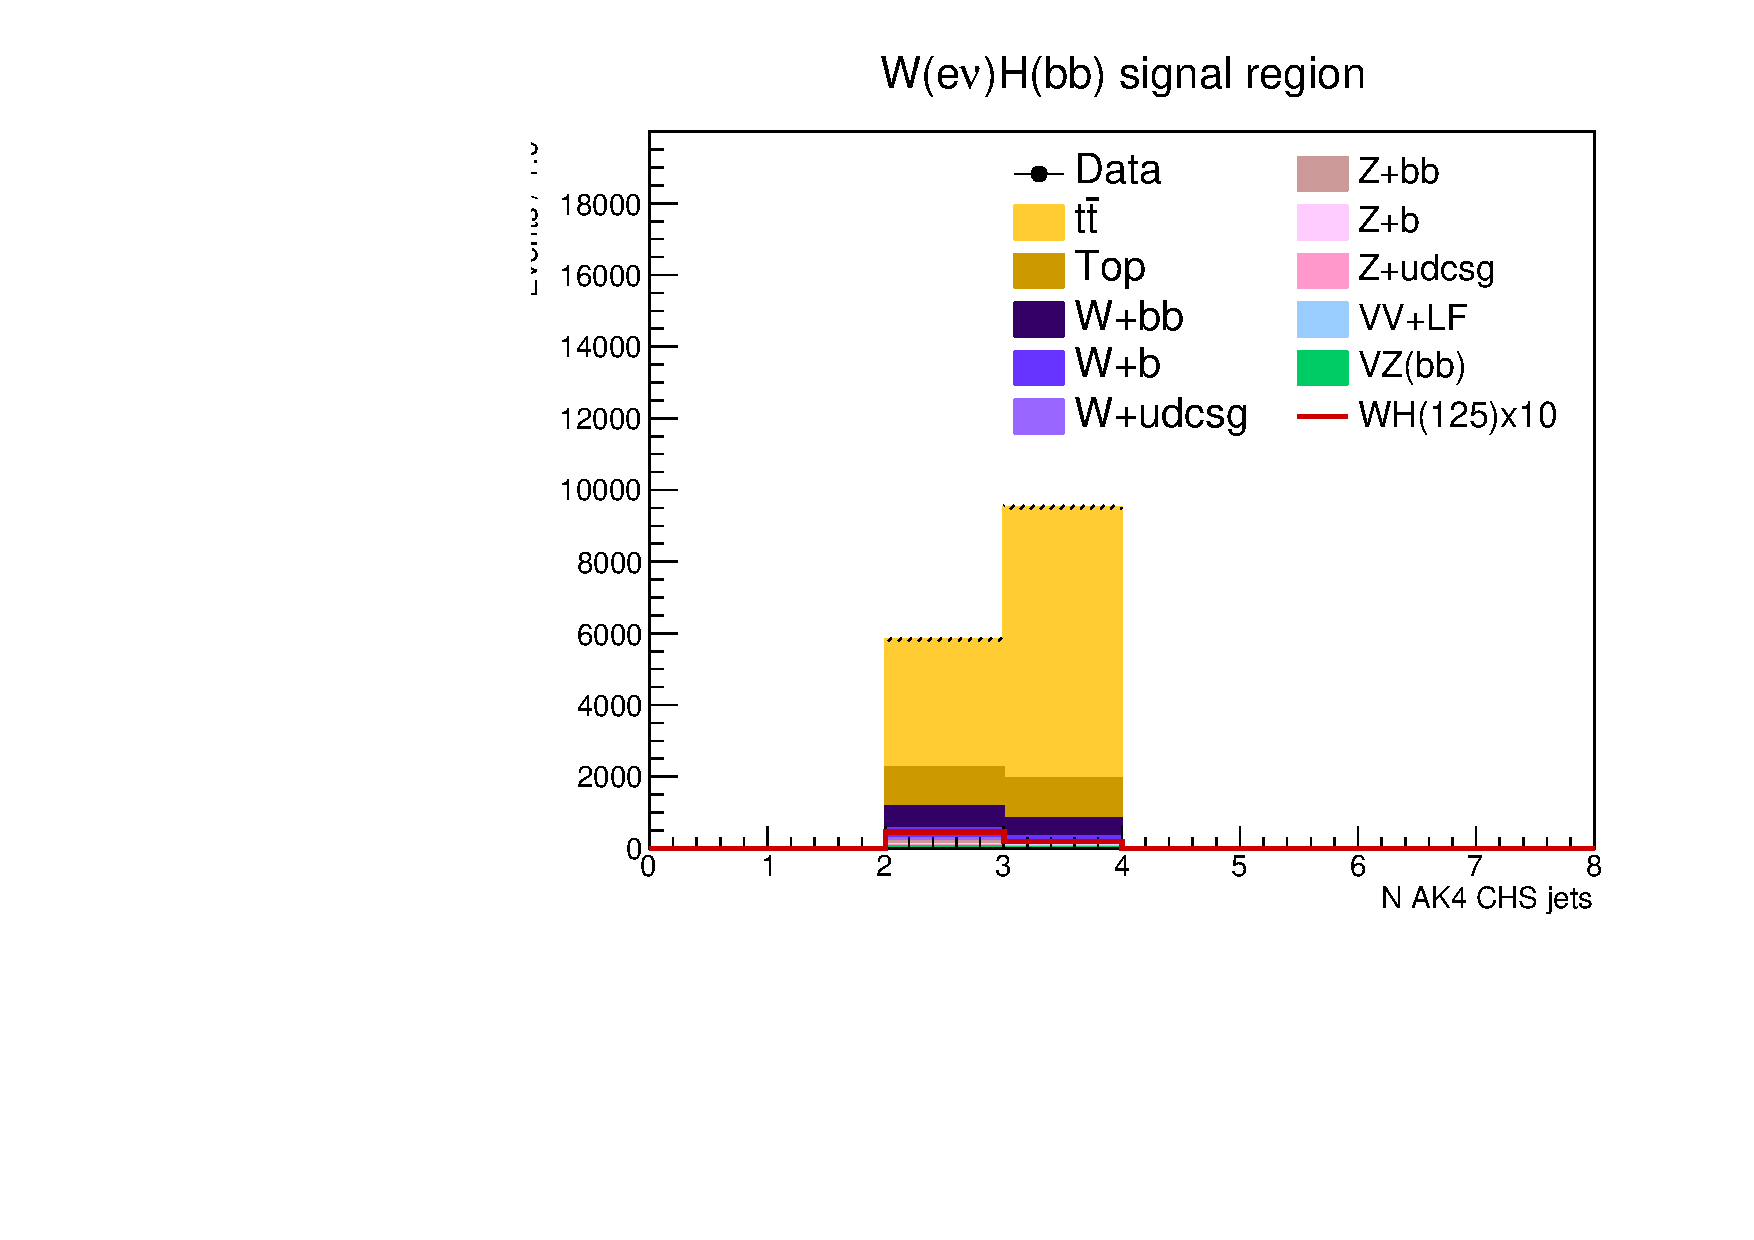
\includegraphics[width=0.48\textwidth]{figures/wlnhbb2016/resolved/WenWHSR_nJet.pdf}
    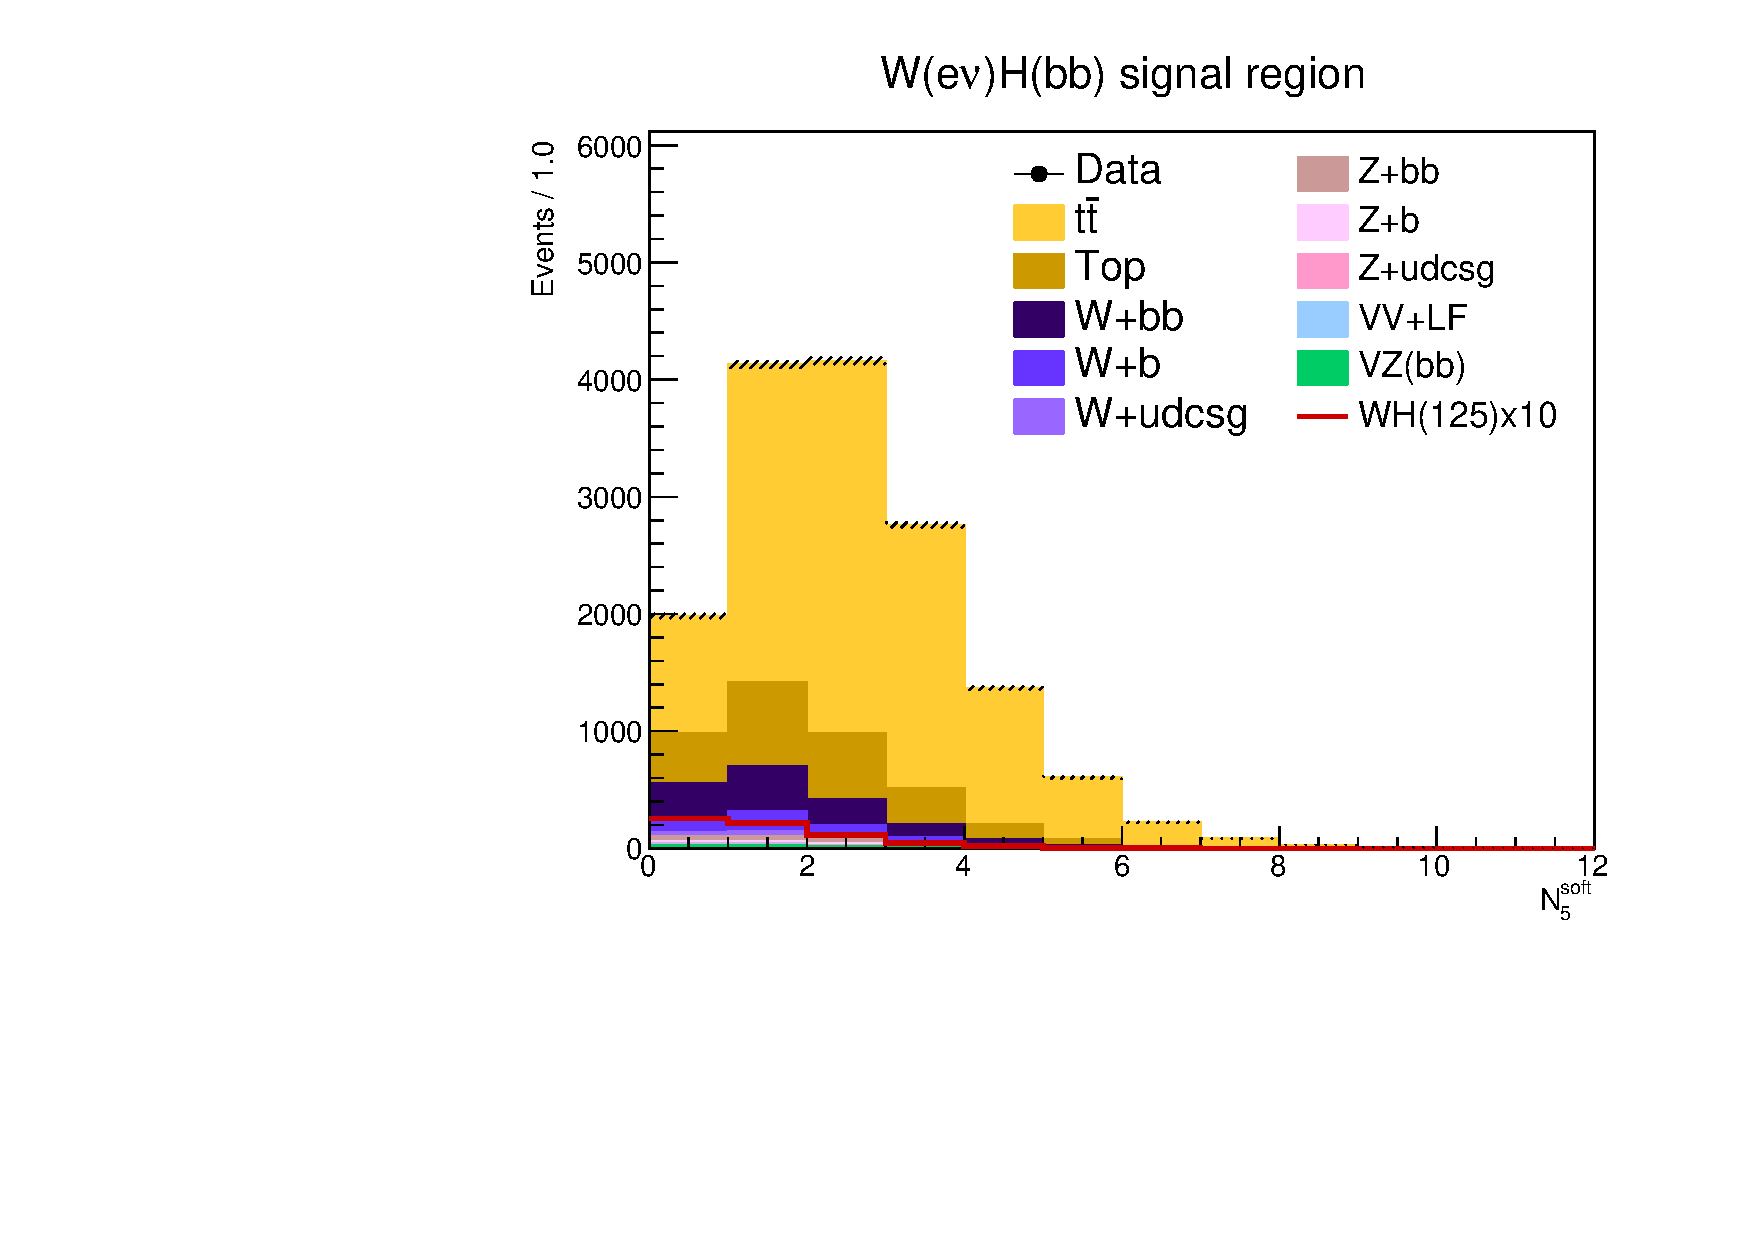
\includegraphics[width=0.48\textwidth]{figures/wlnhbb2016/resolved/WenWHSR_nSoft5.pdf}
    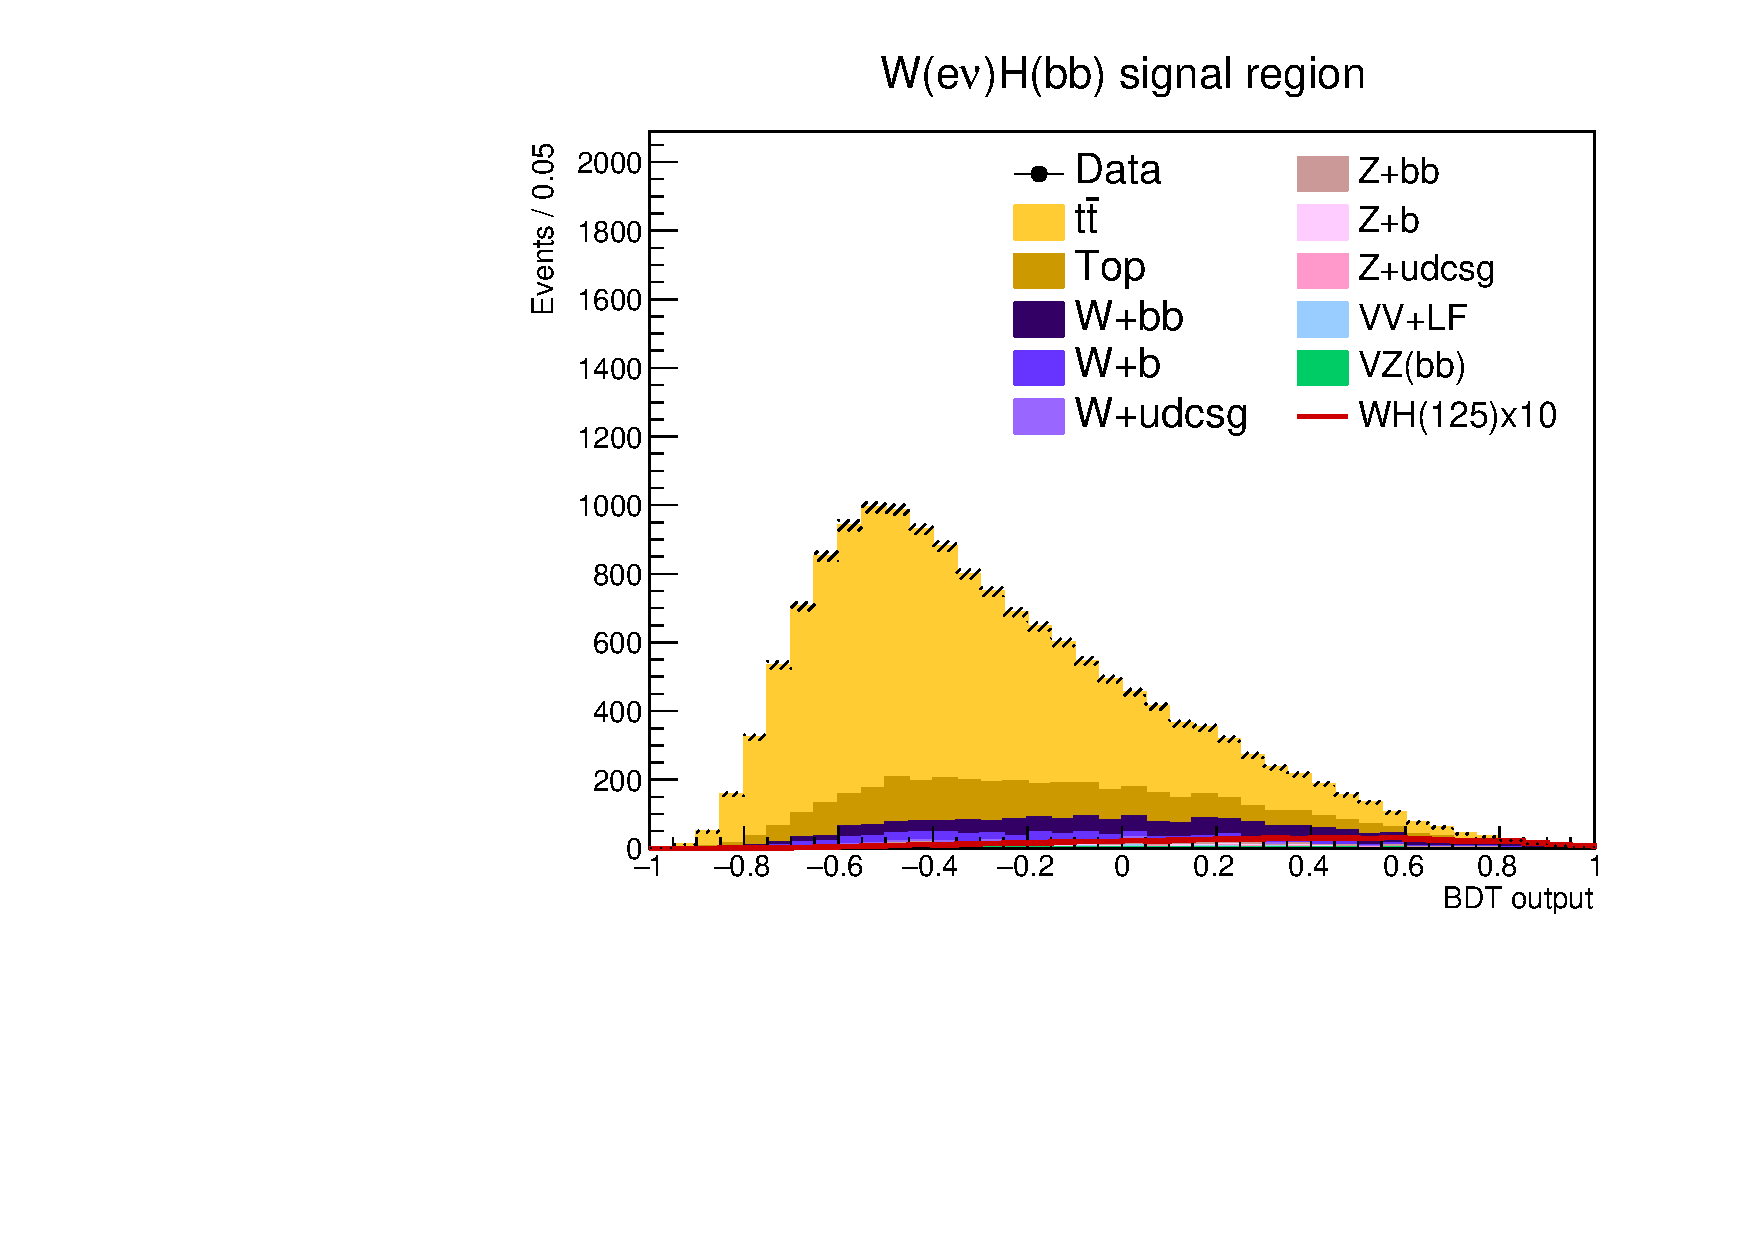
\includegraphics[width=0.48\textwidth]{figures/wlnhbb2016/resolved/WenWHSR_bdtValue.pdf}
    \caption{WH kinematics in the resolved category W(e$\nu$) signal region.
    Left to right and top to bottom: WH $\pt$ balance, WH azimuthal separation, leading b-tag score, the number of central jets,
    the number of 5 \GeV\ soft activity jets, and the evaluation of the signal extraction BDT.
    The simulated shapes are prefit, with the postfit normalizations applied.}
    \label{fig:res_WenSR_WH}
  \end{center}
\end{figure}
\clearpage


\begin{figure}[tbp]
  \begin{center}
    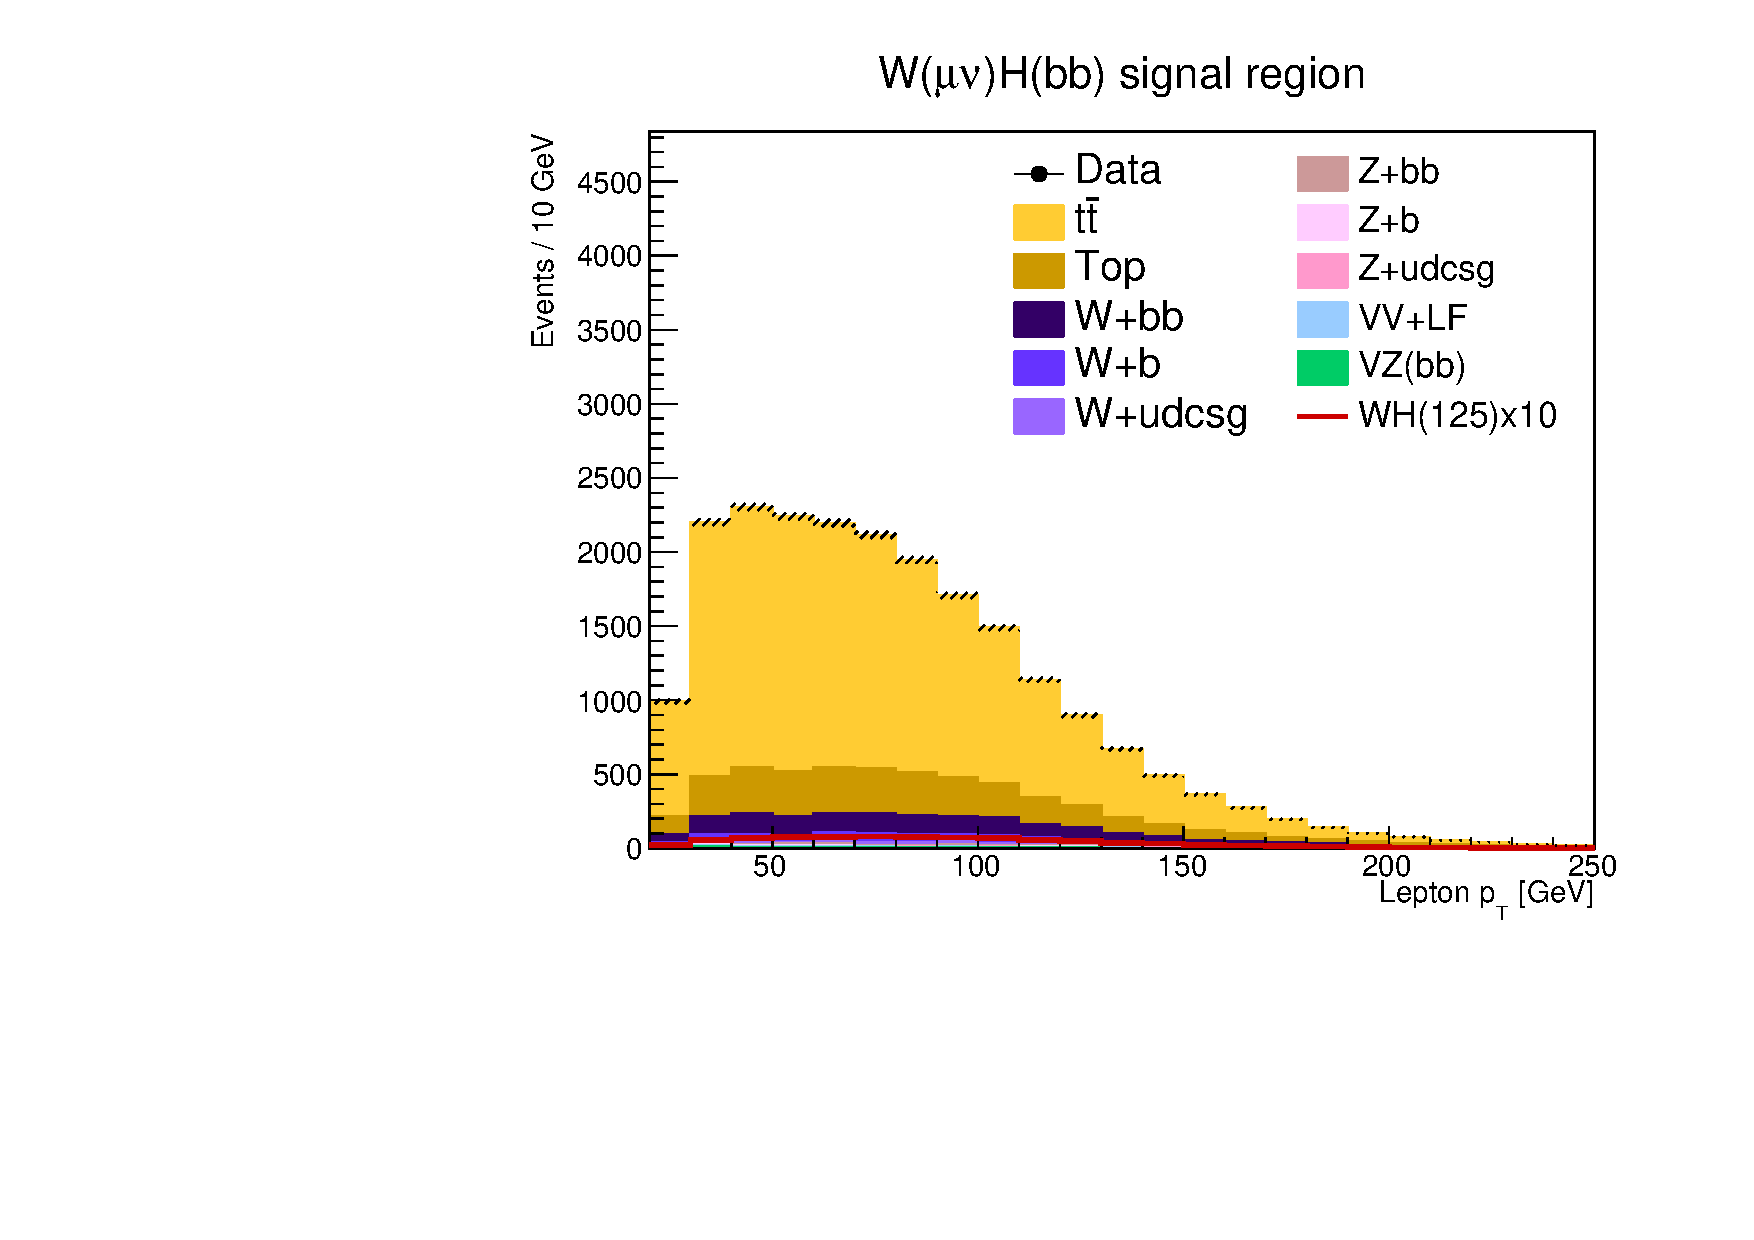
\includegraphics[width=0.48\textwidth]{figures/wlnhbb2016/resolved/WmnWHSR_lepton1Pt.pdf}
    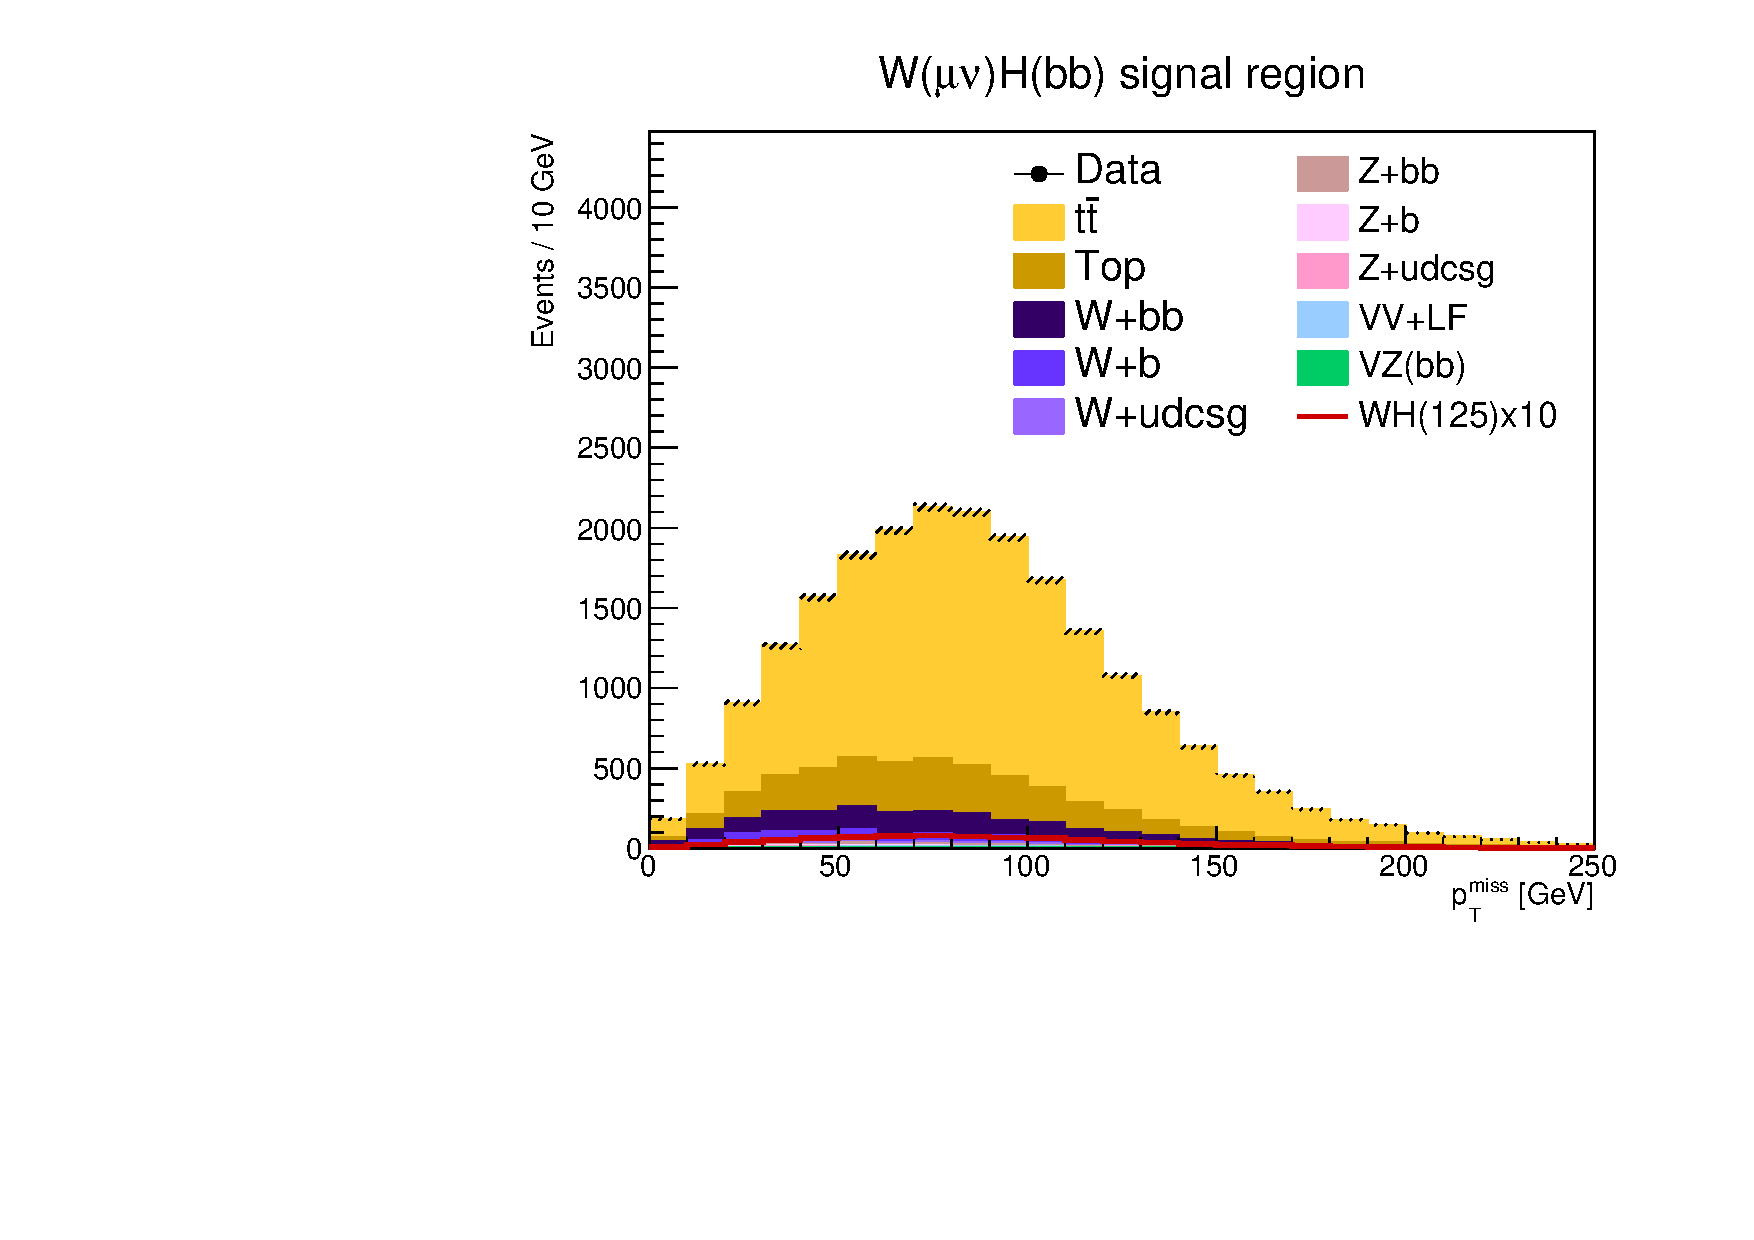
\includegraphics[width=0.48\textwidth]{figures/wlnhbb2016/resolved/WmnWHSR_pfmet.pdf}
    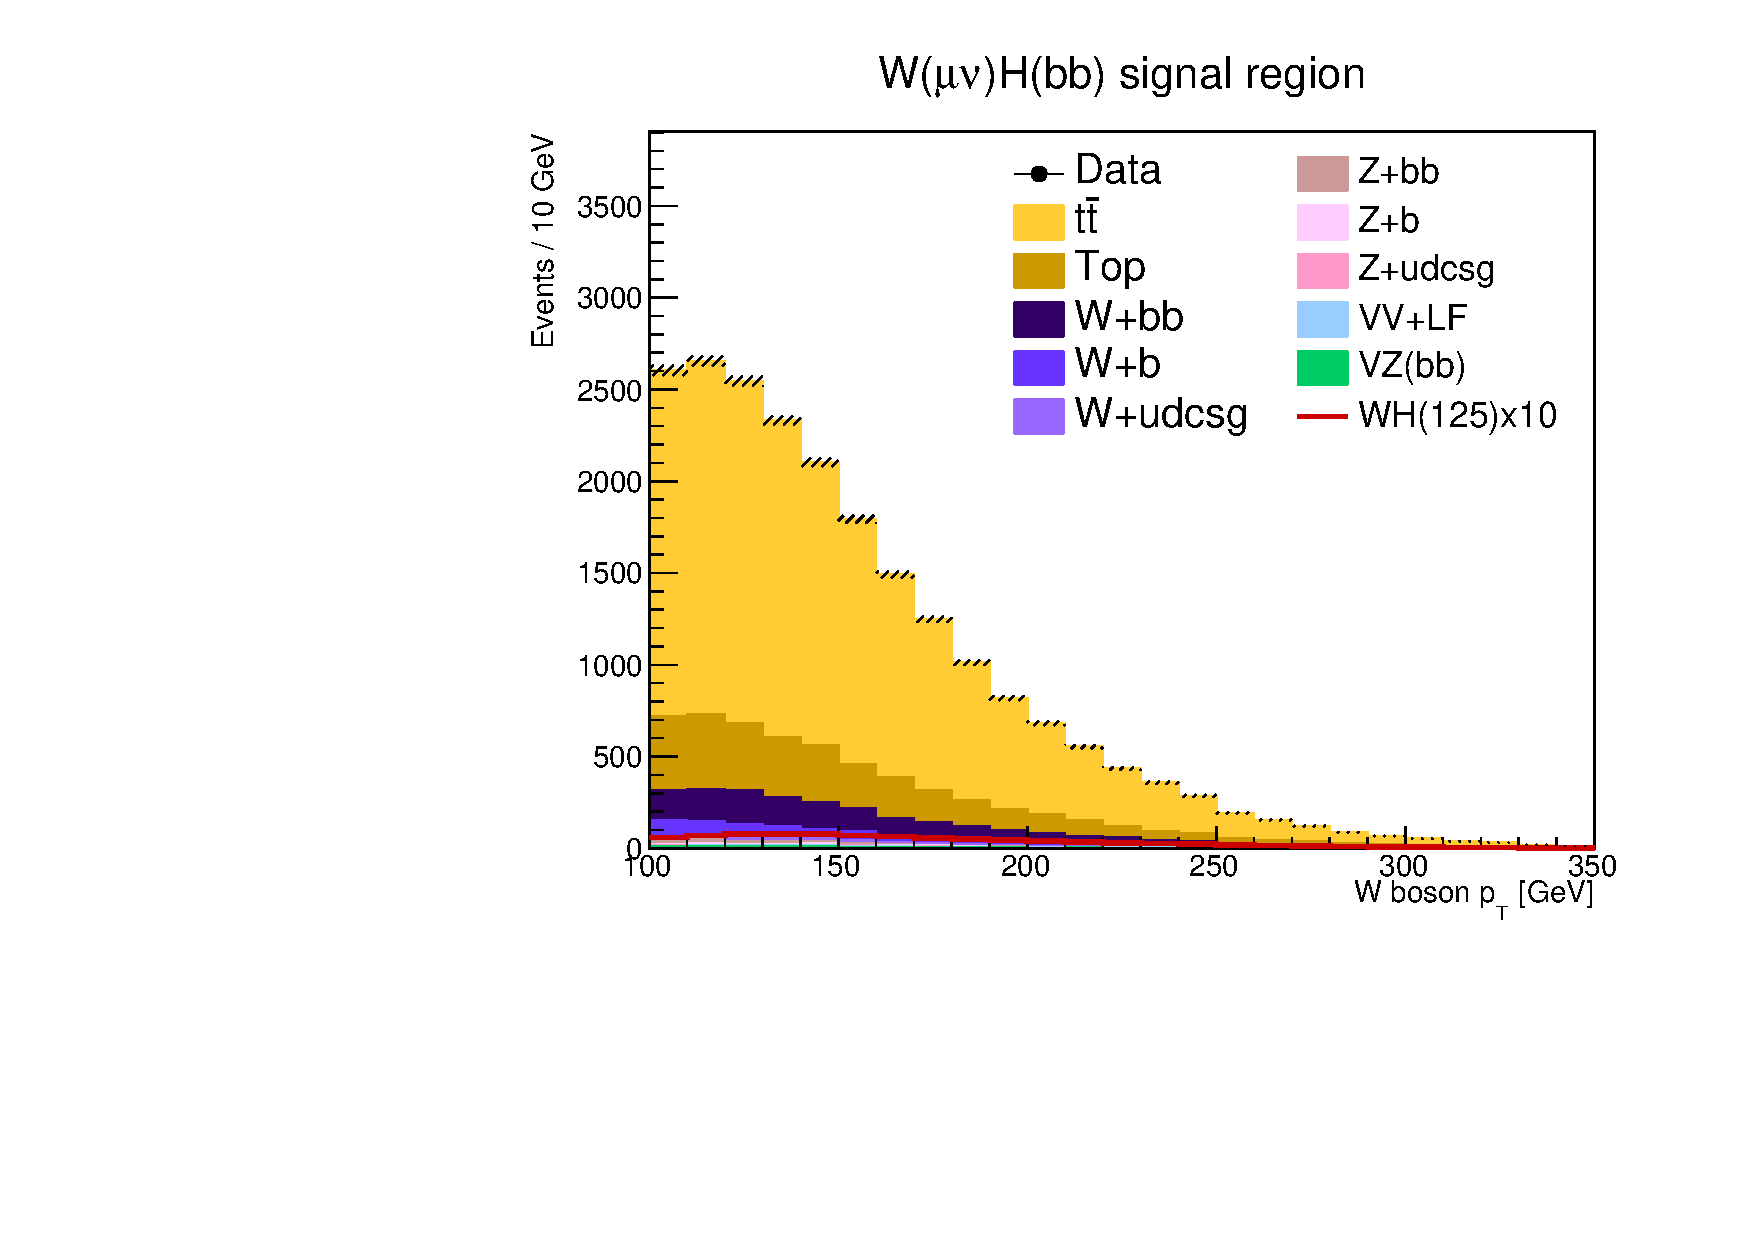
\includegraphics[width=0.48\textwidth]{figures/wlnhbb2016/resolved/WmnWHSR_WpT.pdf}
    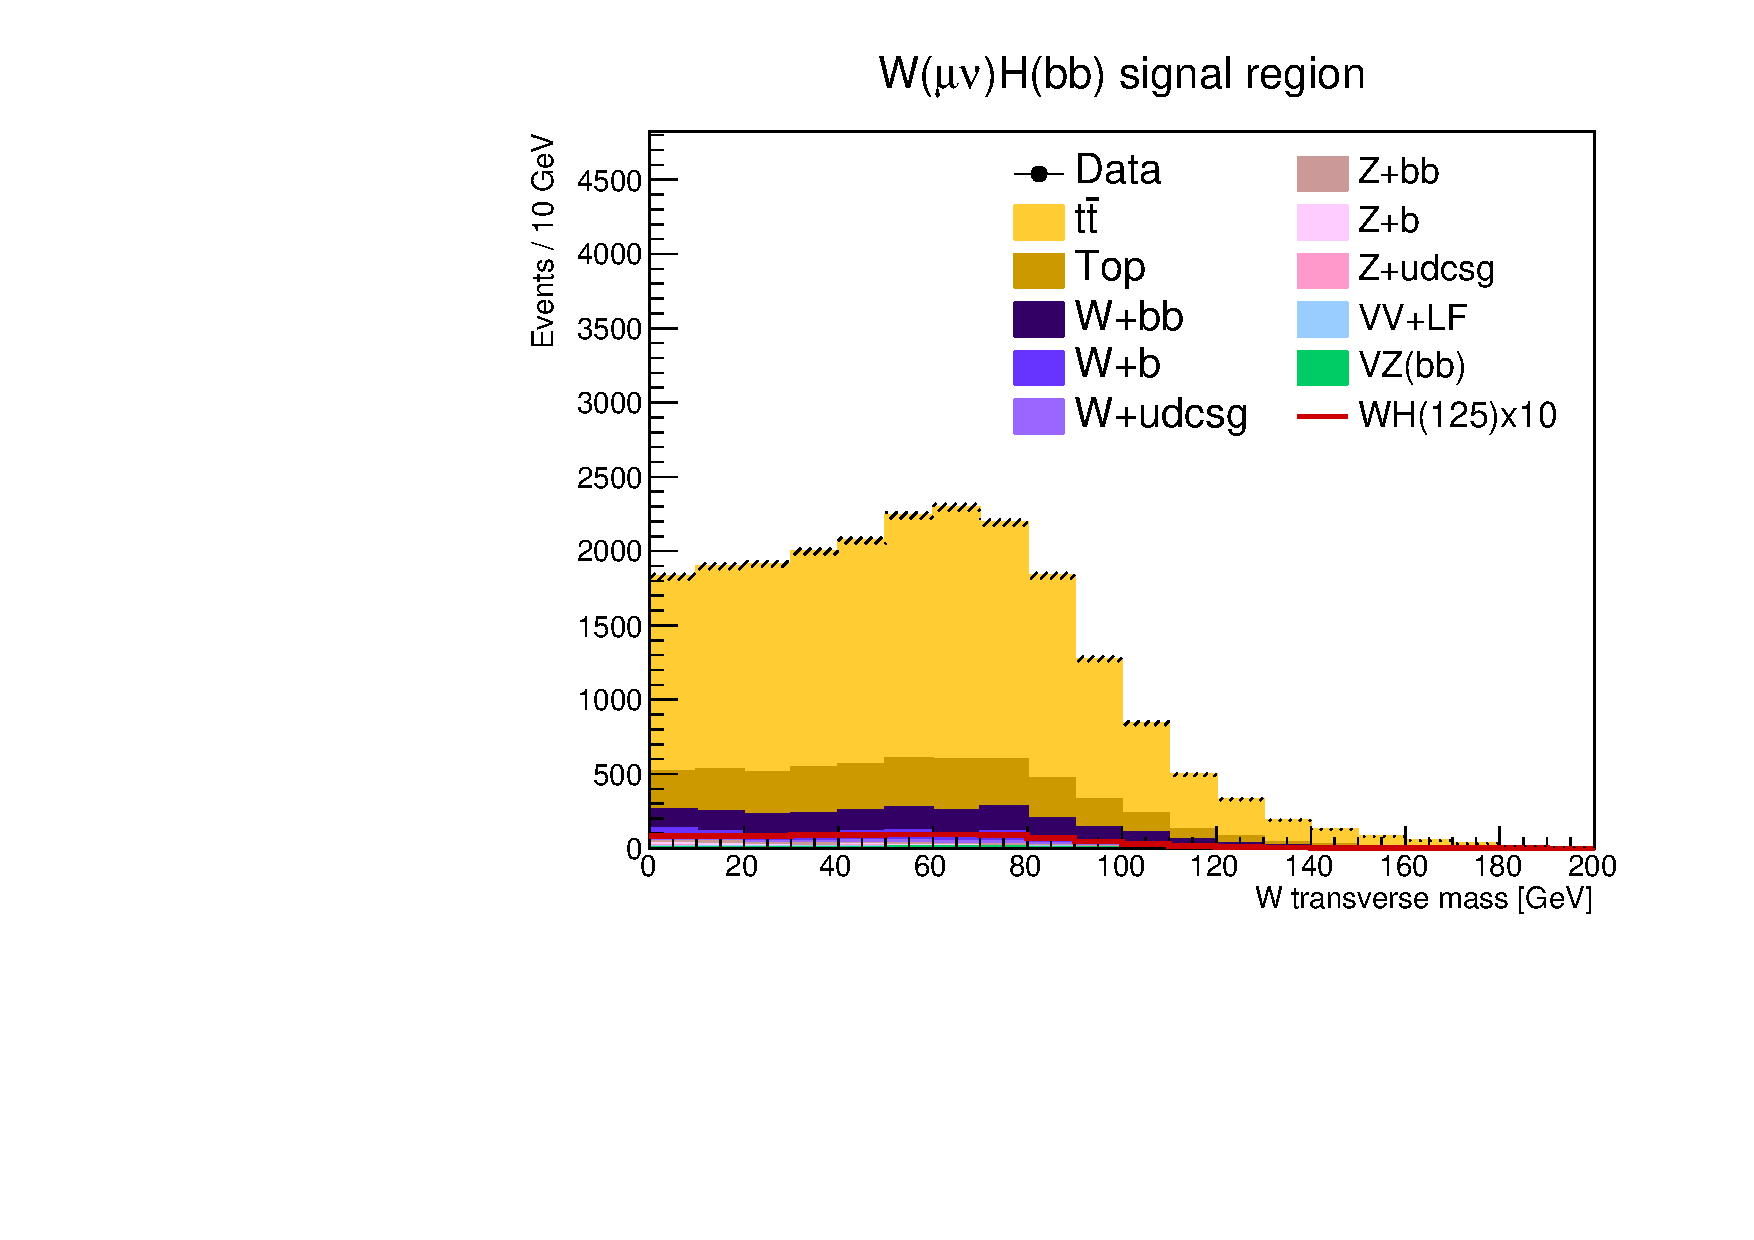
\includegraphics[width=0.48\textwidth]{figures/wlnhbb2016/resolved/WmnWHSR_mTW.pdf}
    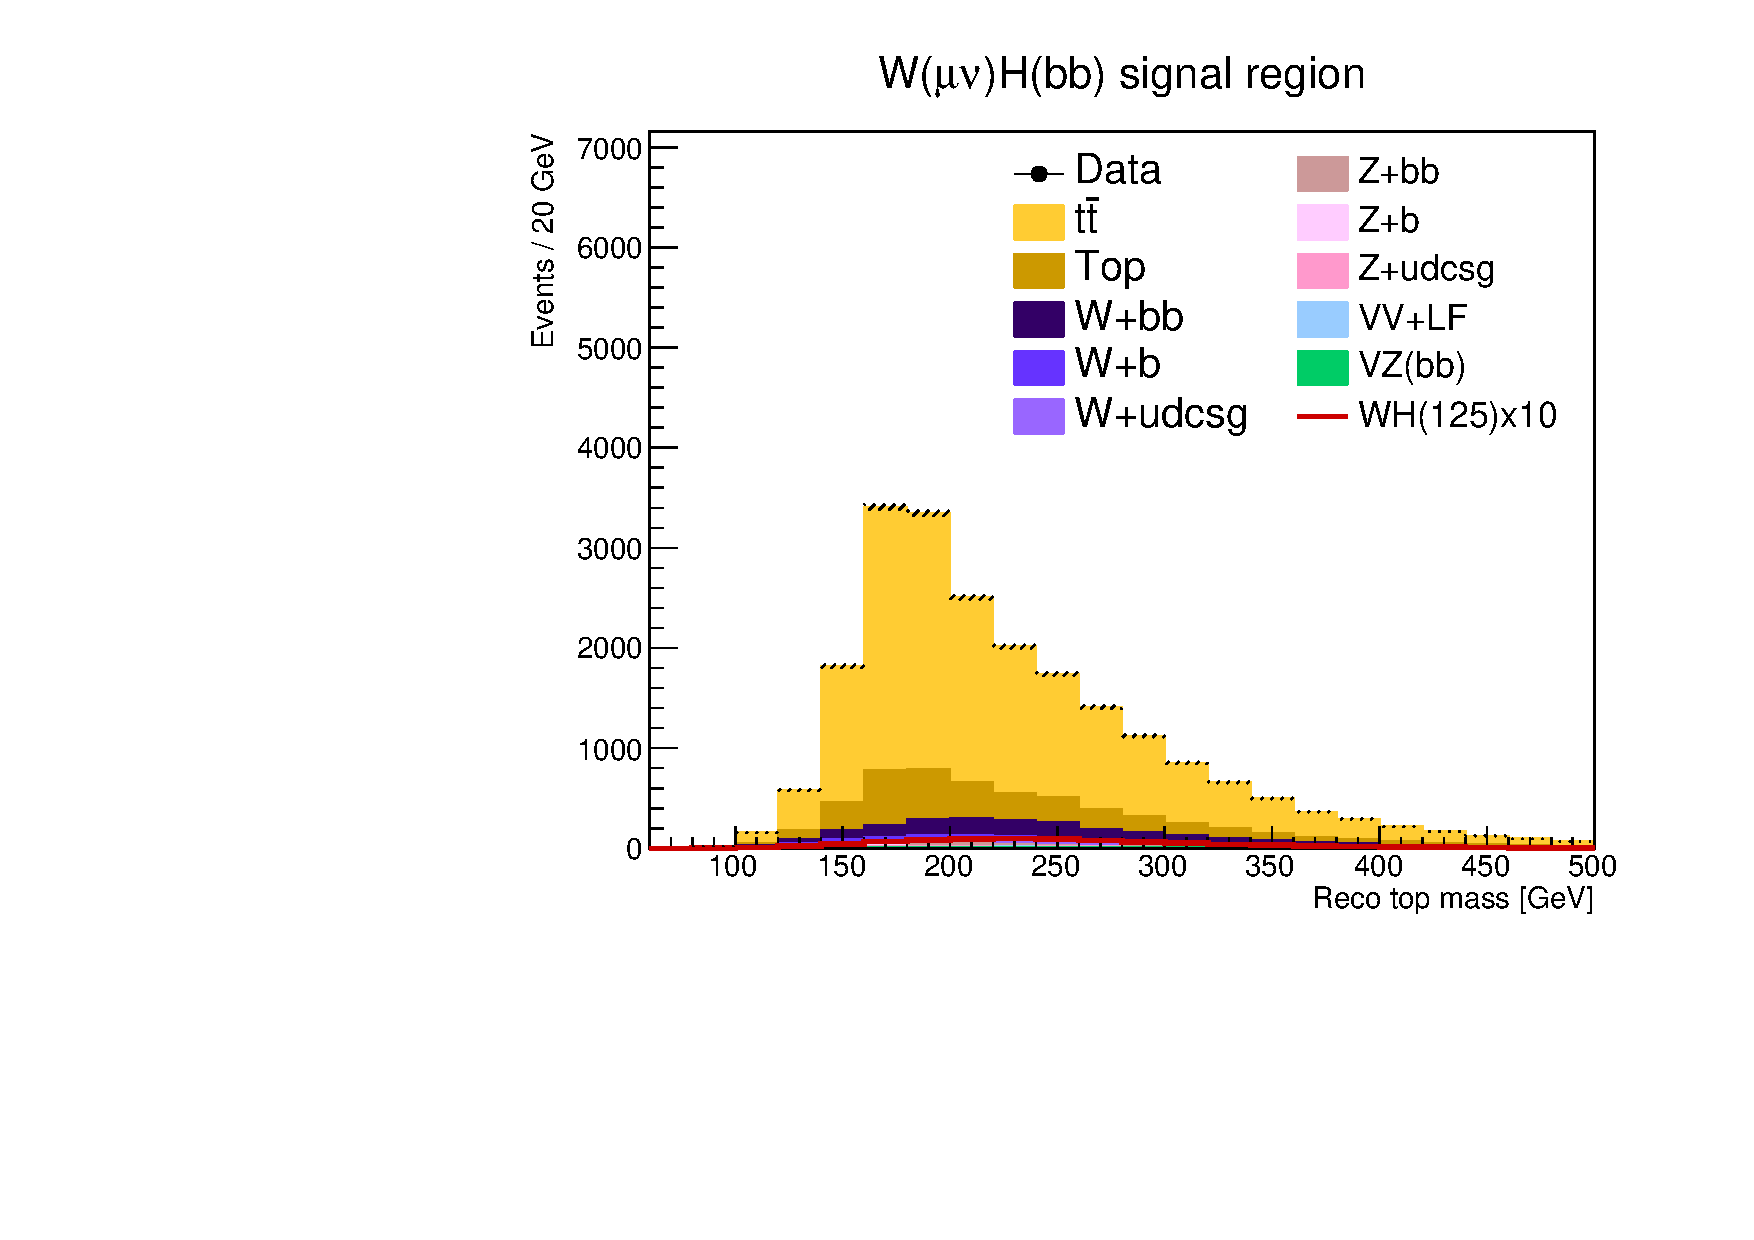
\includegraphics[width=0.48\textwidth]{figures/wlnhbb2016/resolved/WmnWHSR_topMassLep1Met.pdf}
    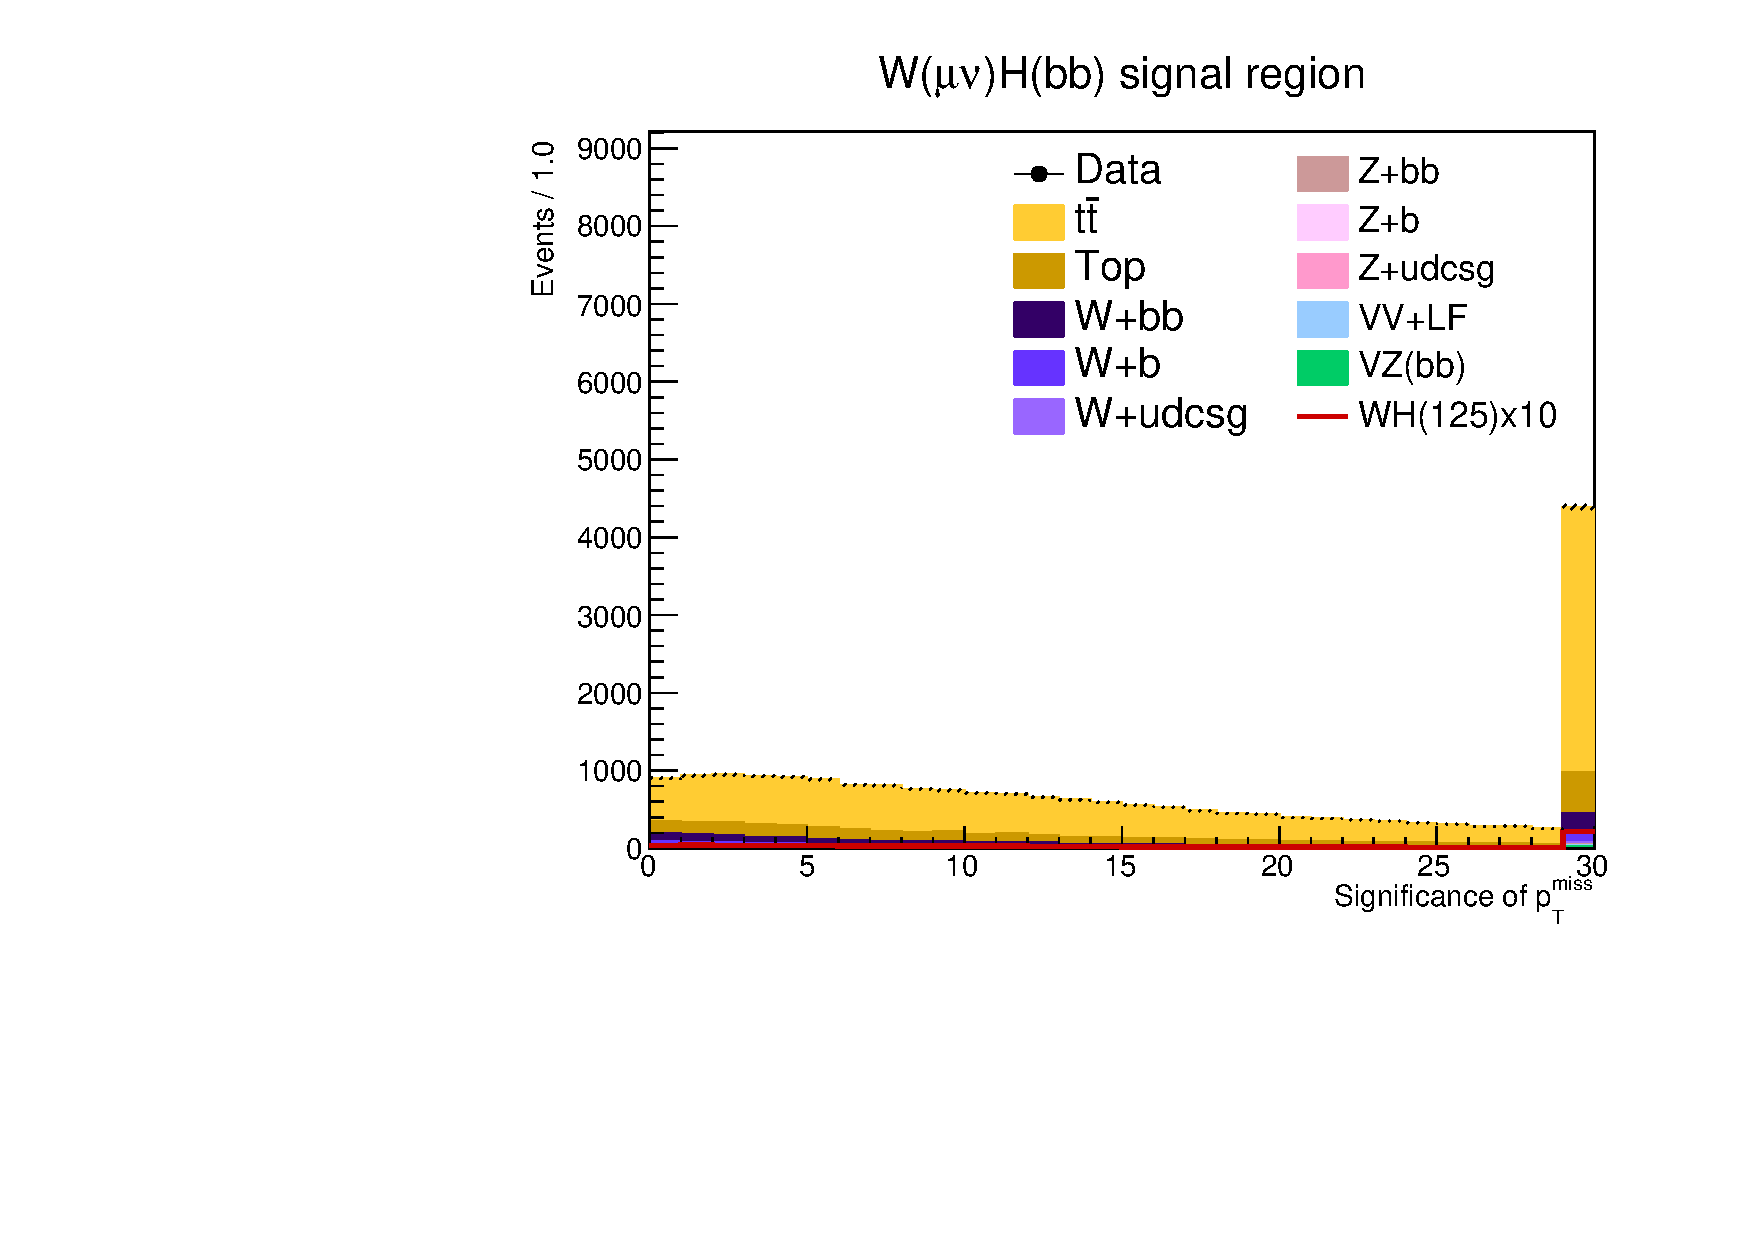
\includegraphics[width=0.48\textwidth]{figures/wlnhbb2016/resolved/WmnWHSR_pfmetsig.pdf}
    \caption{W boson reconstruction in the resolved category W($\mu\nu$) signal region.
    Left to right and top to bottom: muon $\pt$, $\MET$, W boson $\pt$, W boson transverse mass,
    the reconstructed top quark mass, and the $\MET$ significance.
    The simulated shapes are prefit, with the postfit normalizations applied.}
    \label{fig:res_WmnSR_WBosons}
  \end{center}
\end{figure}
\clearpage

\begin{figure}[tbp]
  \begin{center}
    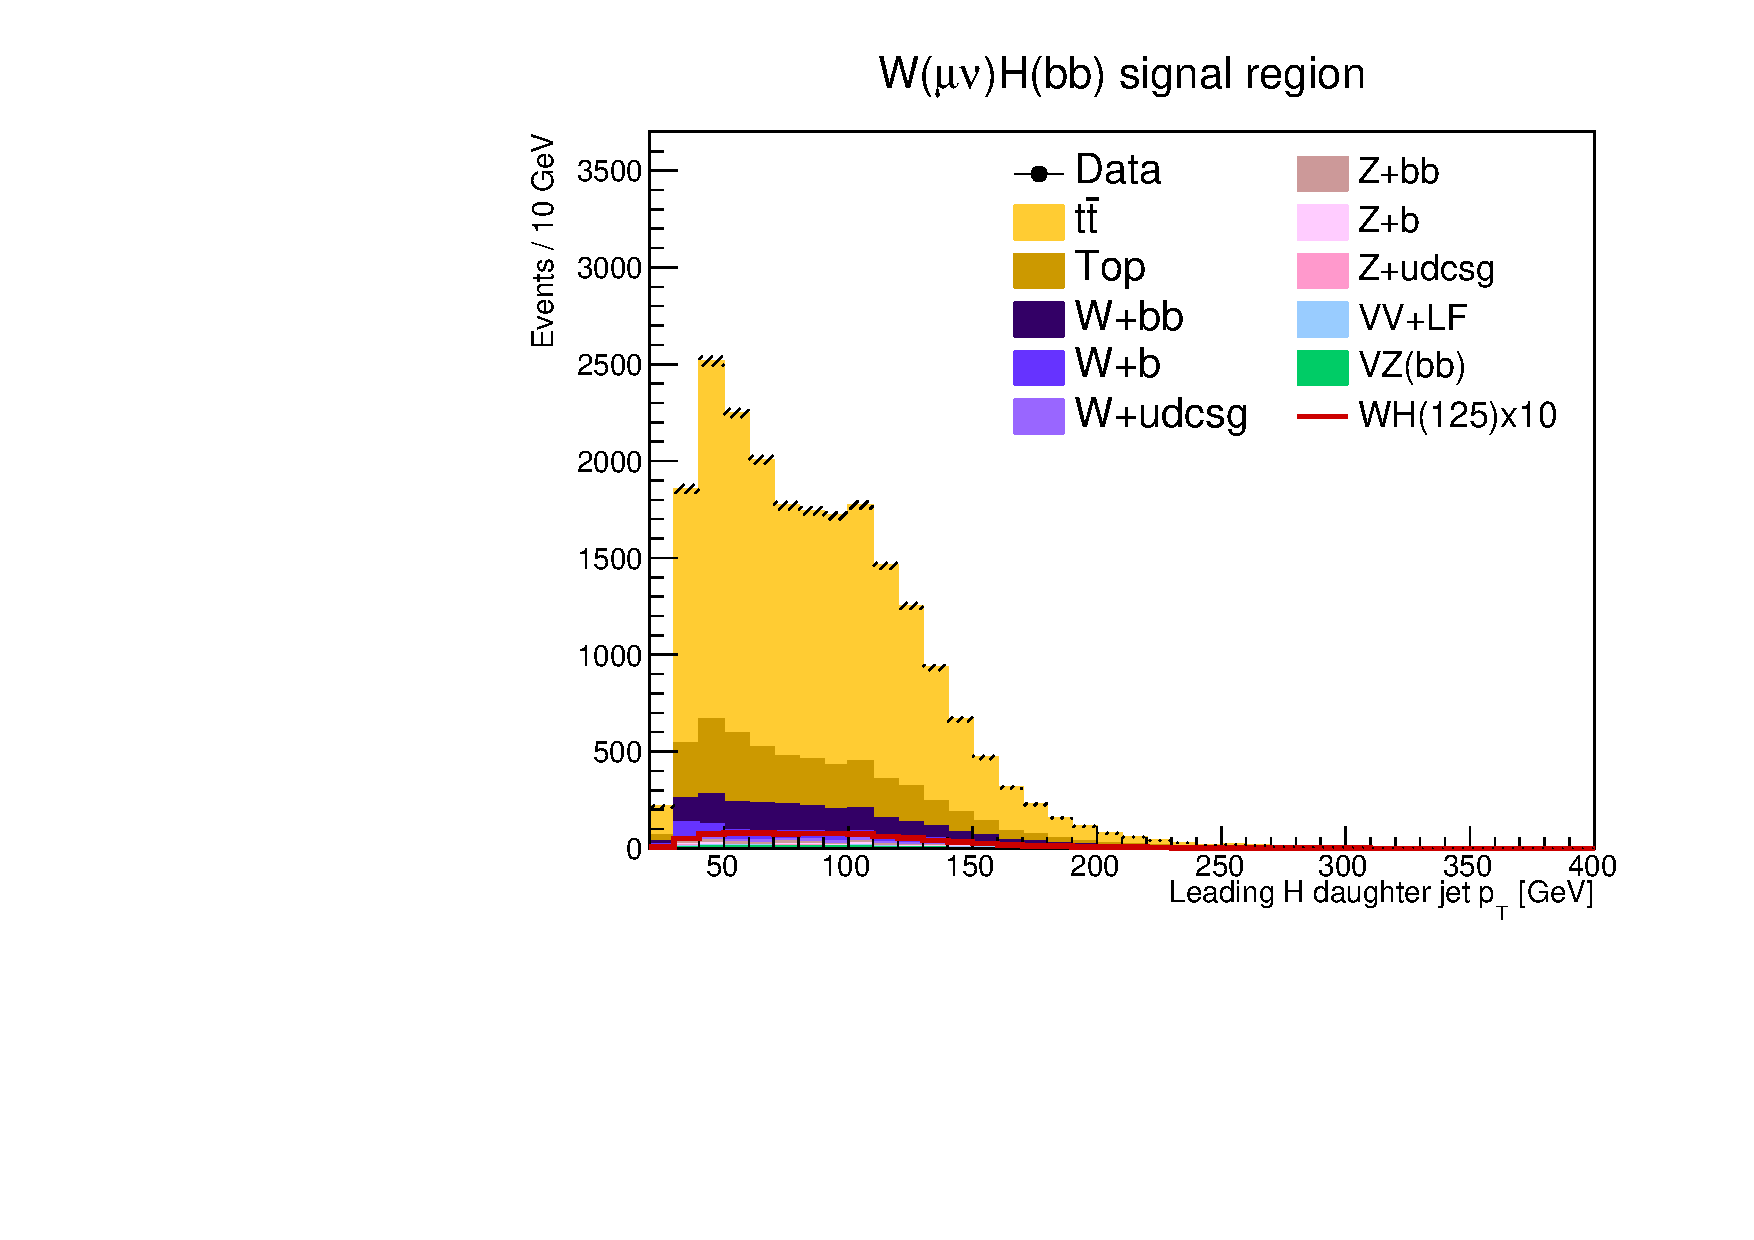
\includegraphics[width=0.48\textwidth]{figures/wlnhbb2016/resolved/WmnWHSR_Hbjet1Pt.pdf}
    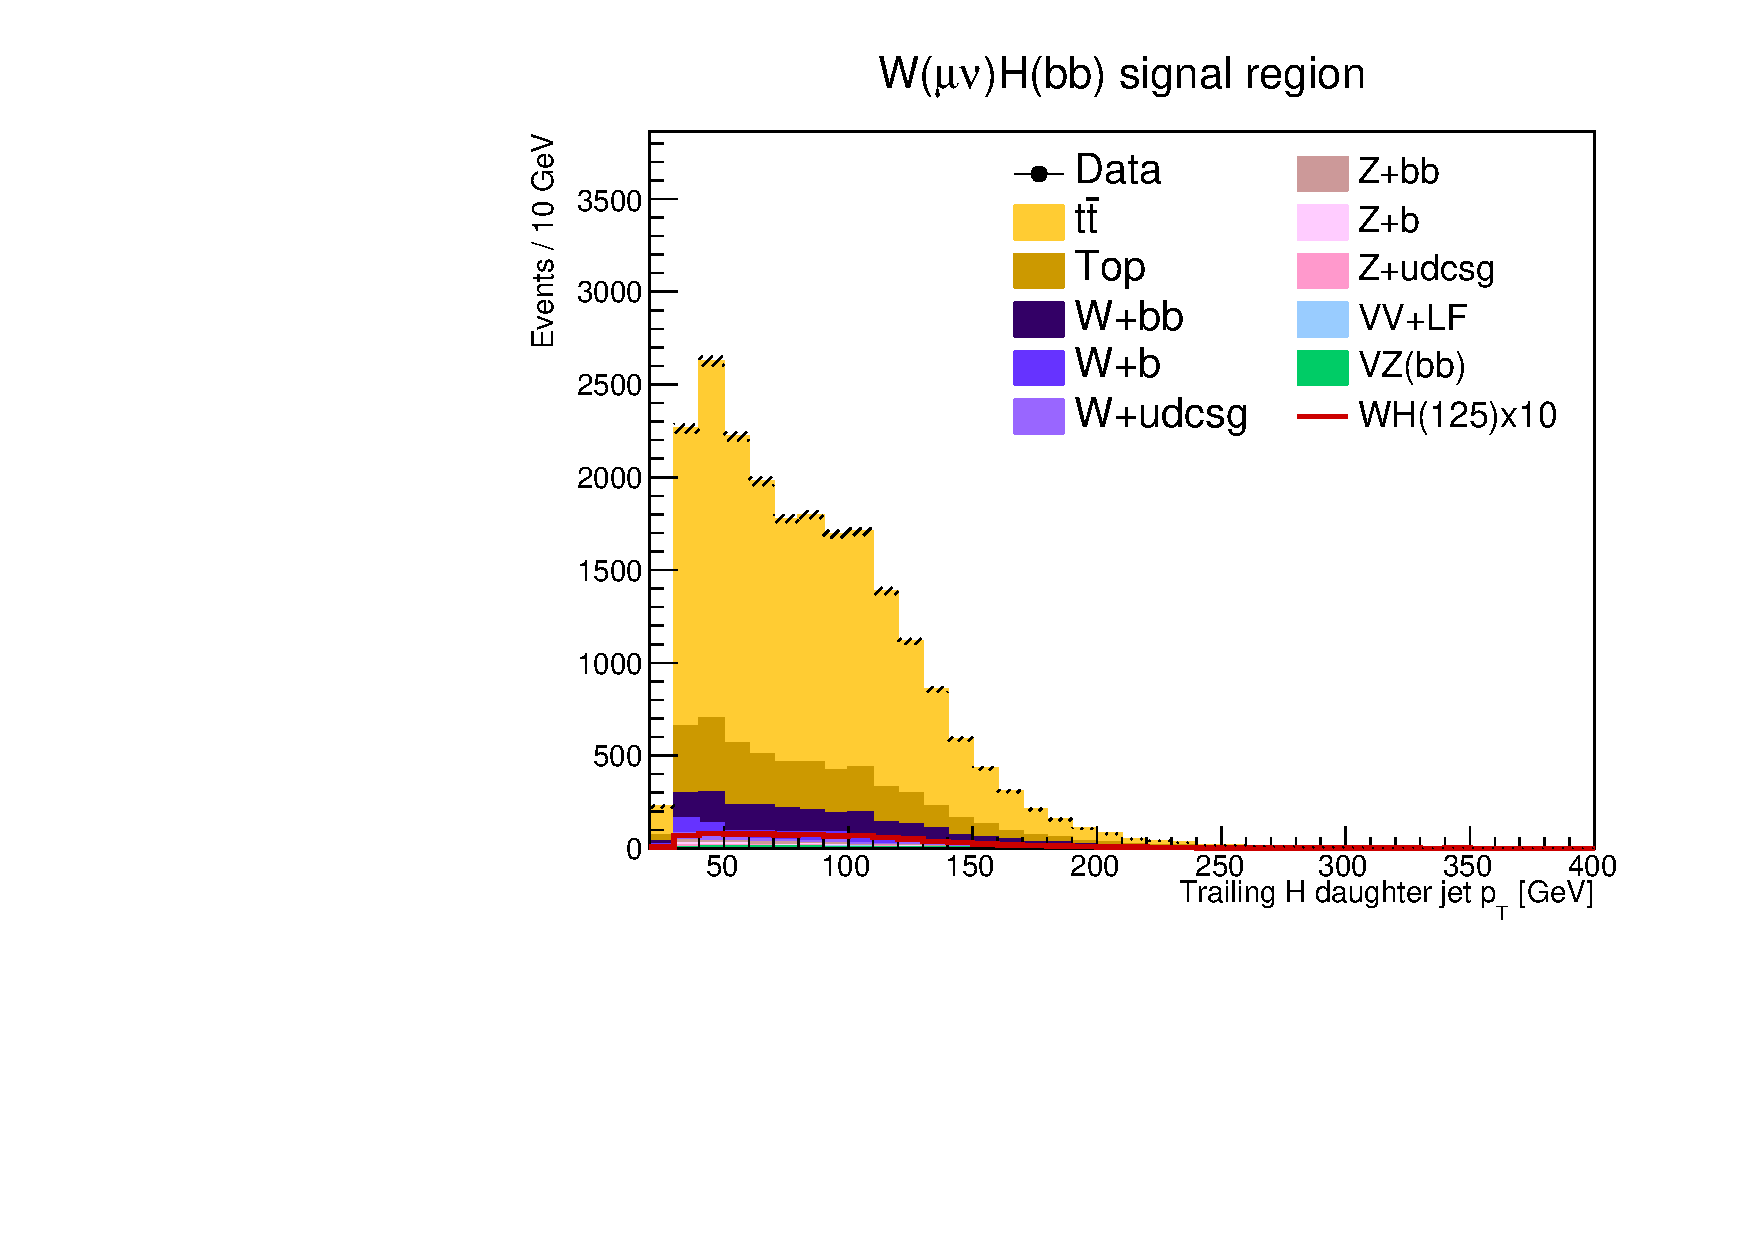
\includegraphics[width=0.48\textwidth]{figures/wlnhbb2016/resolved/WmnWHSR_Hbjet2Pt.pdf}
    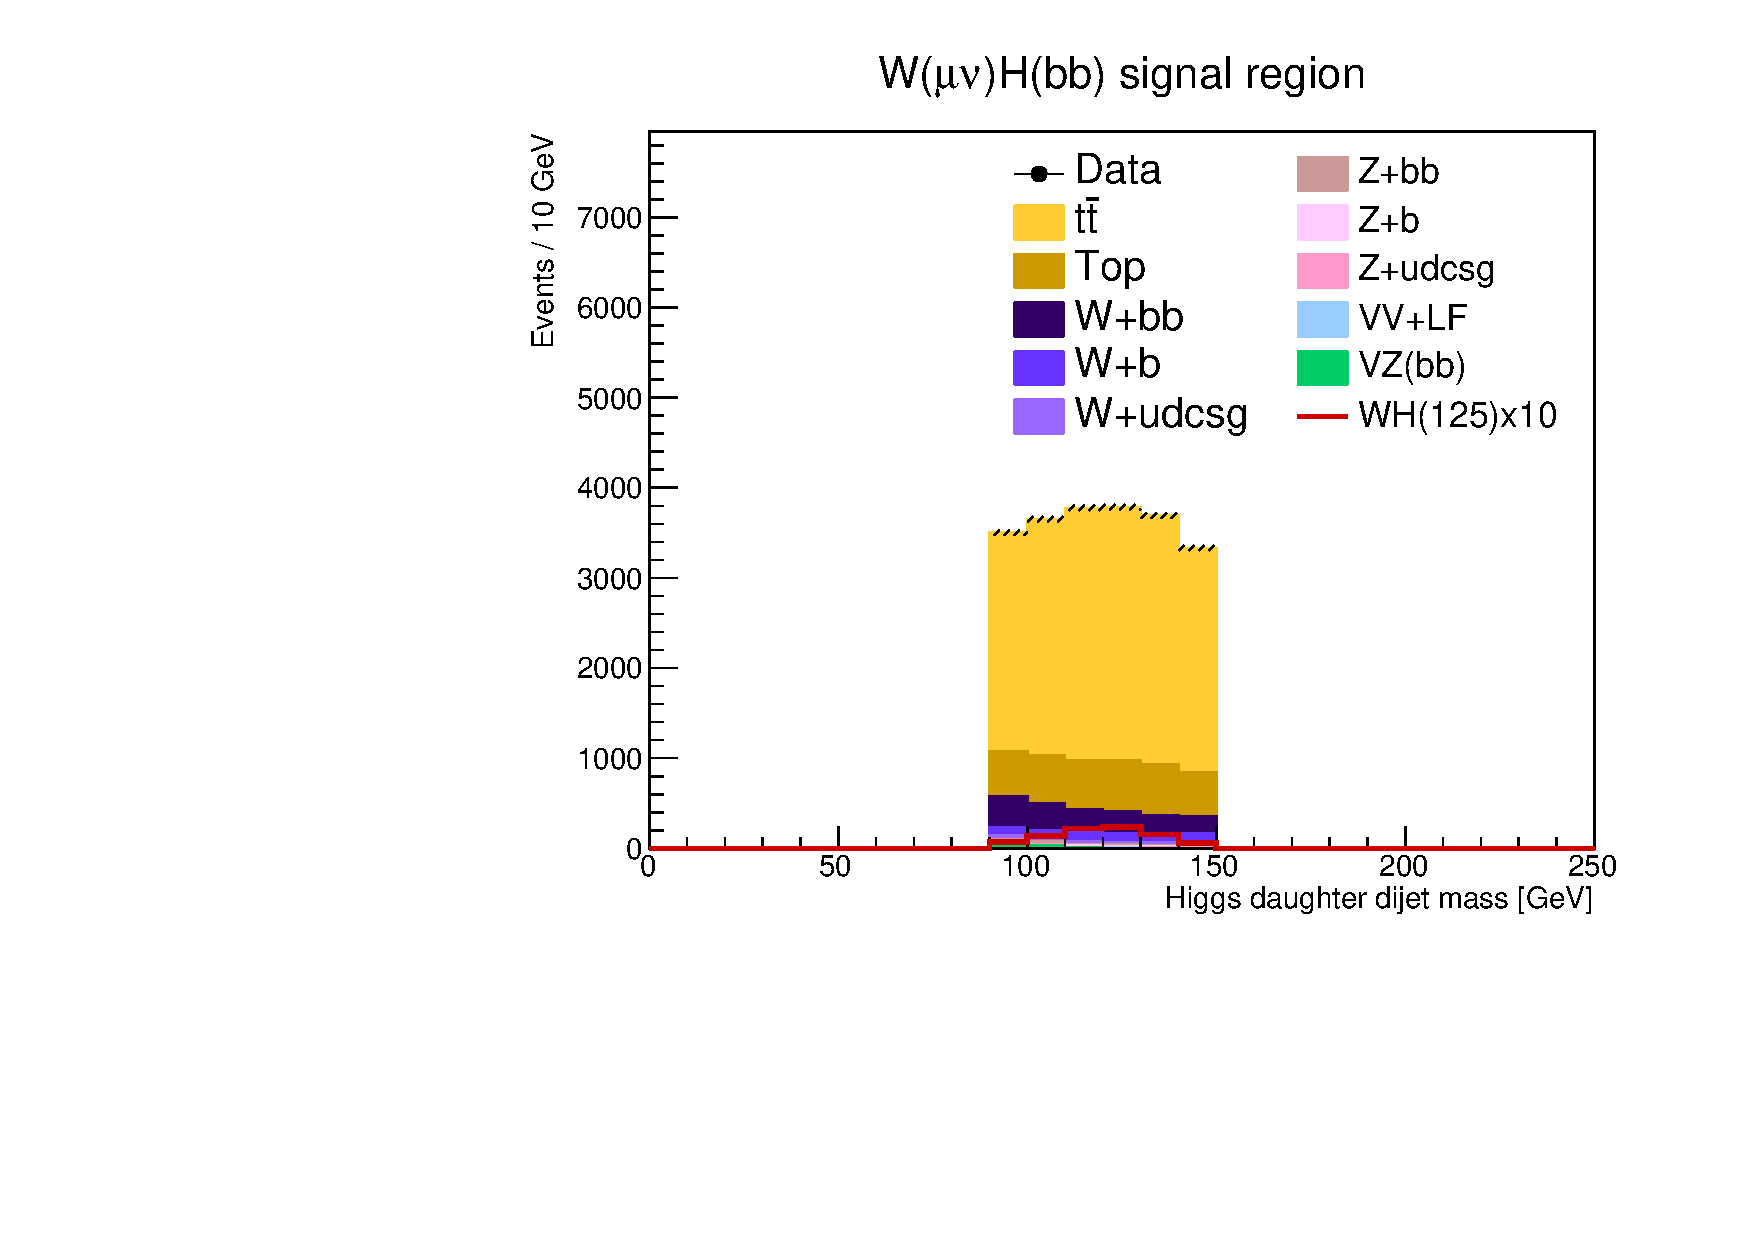
\includegraphics[width=0.48\textwidth]{figures/wlnhbb2016/resolved/WmnWHSR_mH.pdf}
    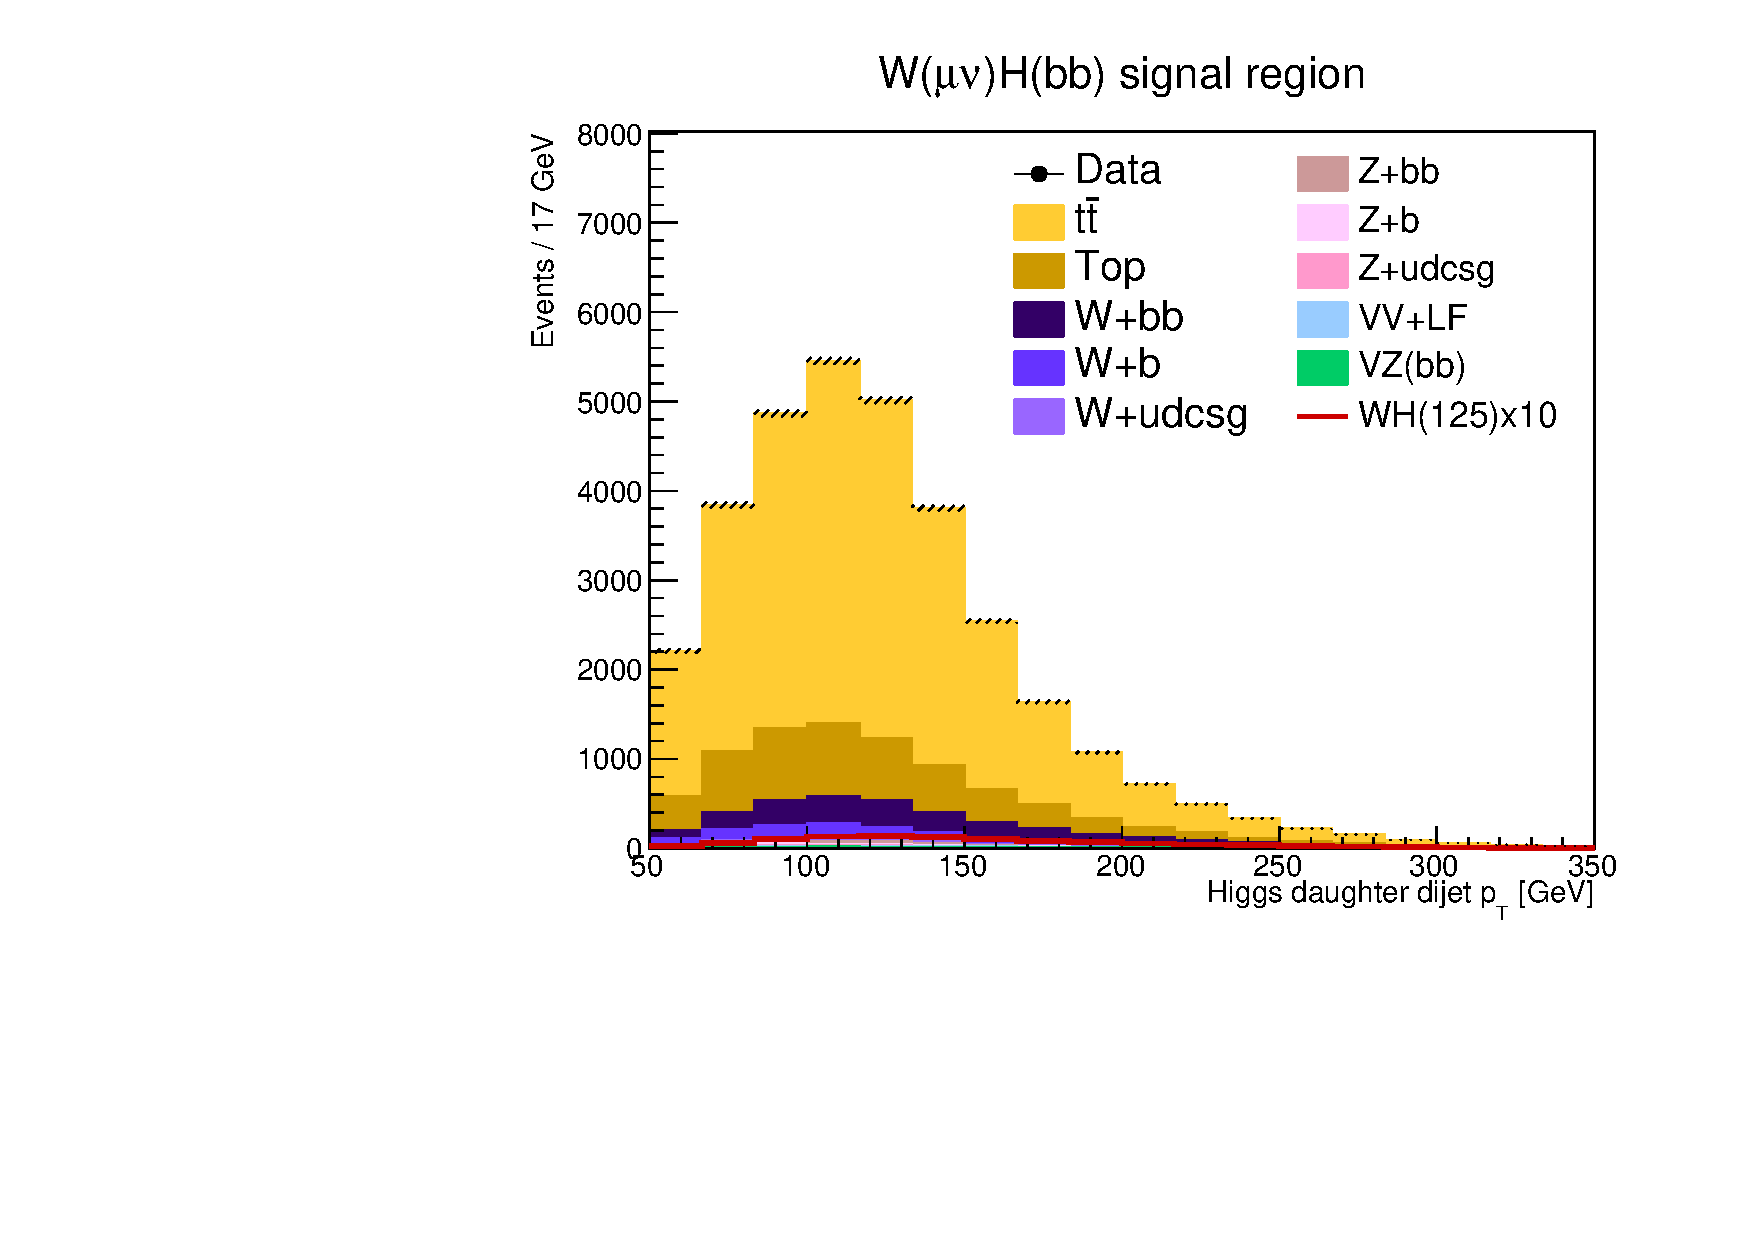
\includegraphics[width=0.48\textwidth]{figures/wlnhbb2016/resolved/WmnWHSR_pTH.pdf}
    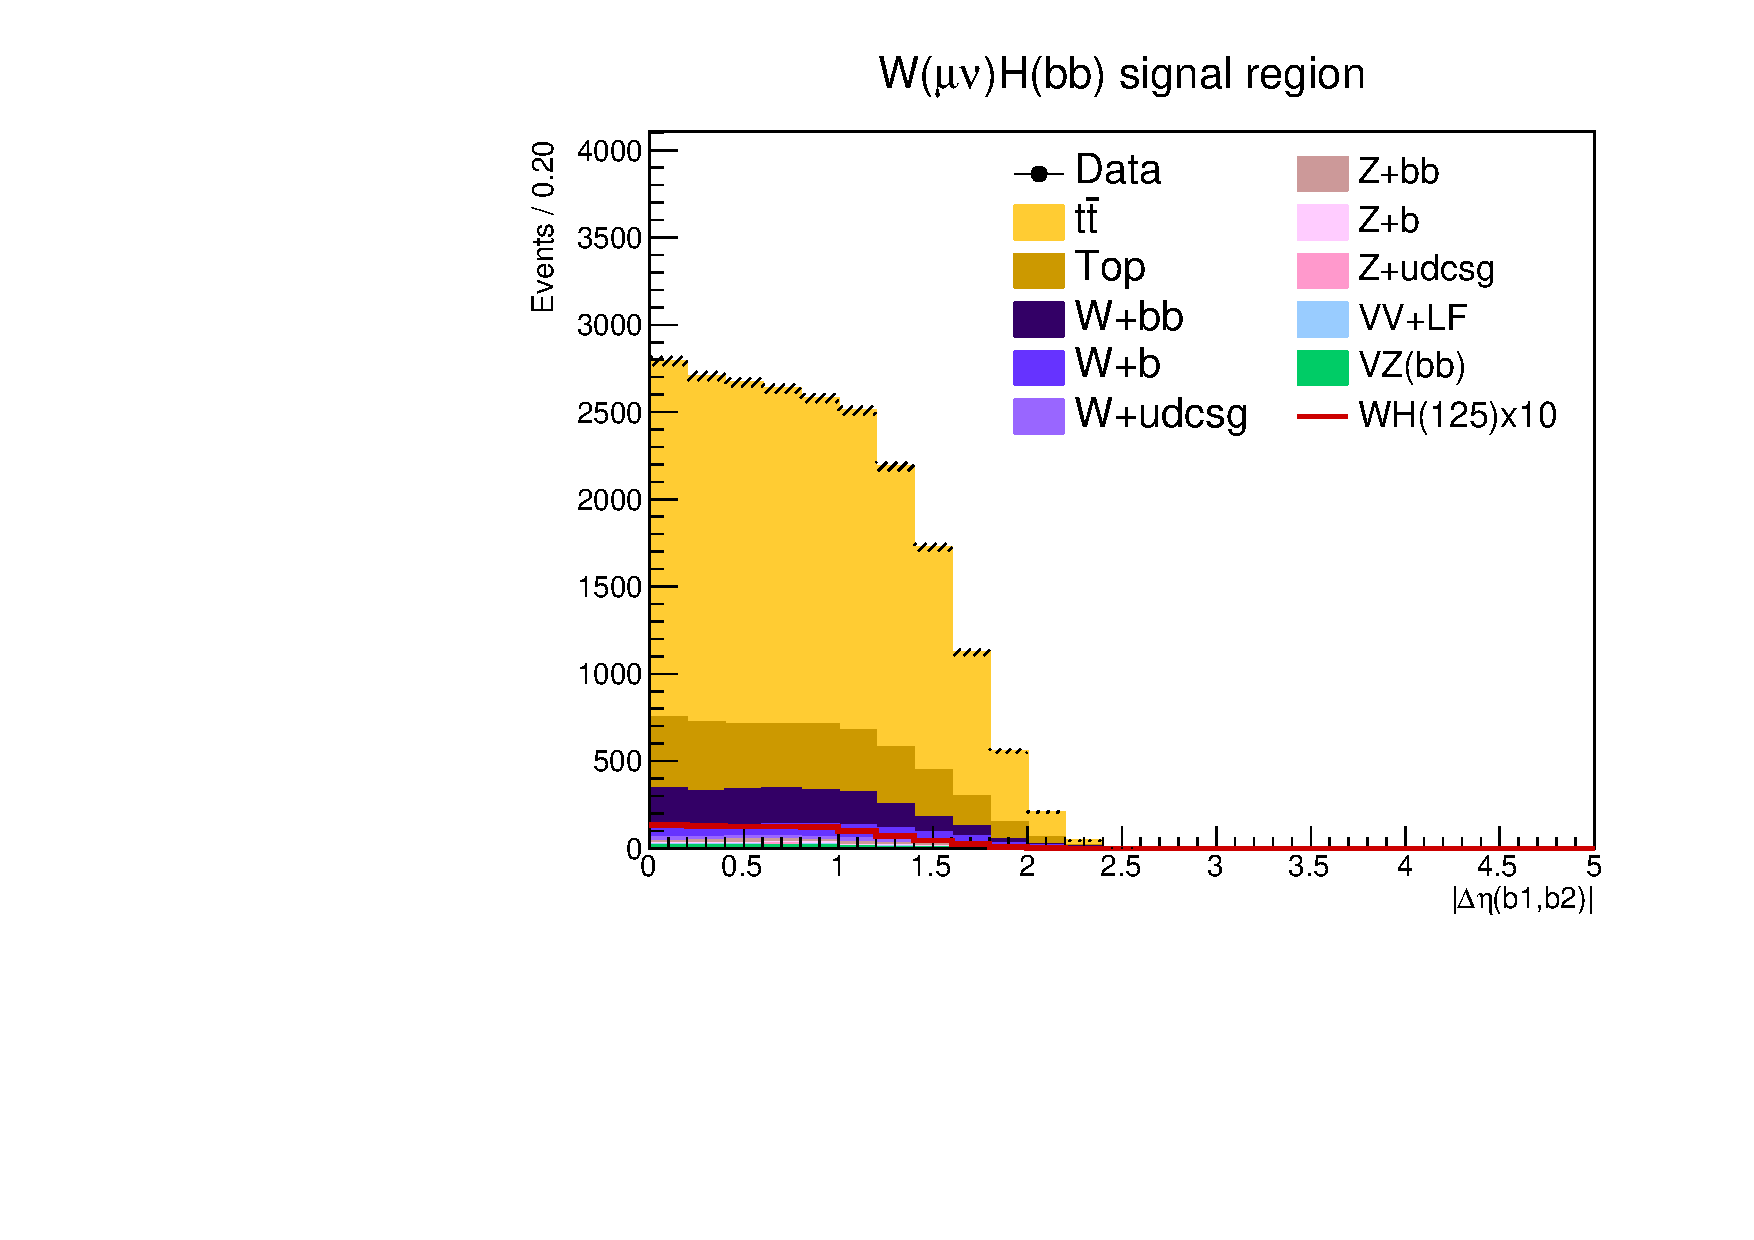
\includegraphics[width=0.48\textwidth]{figures/wlnhbb2016/resolved/WmnWHSR_dEtab1b2.pdf}
    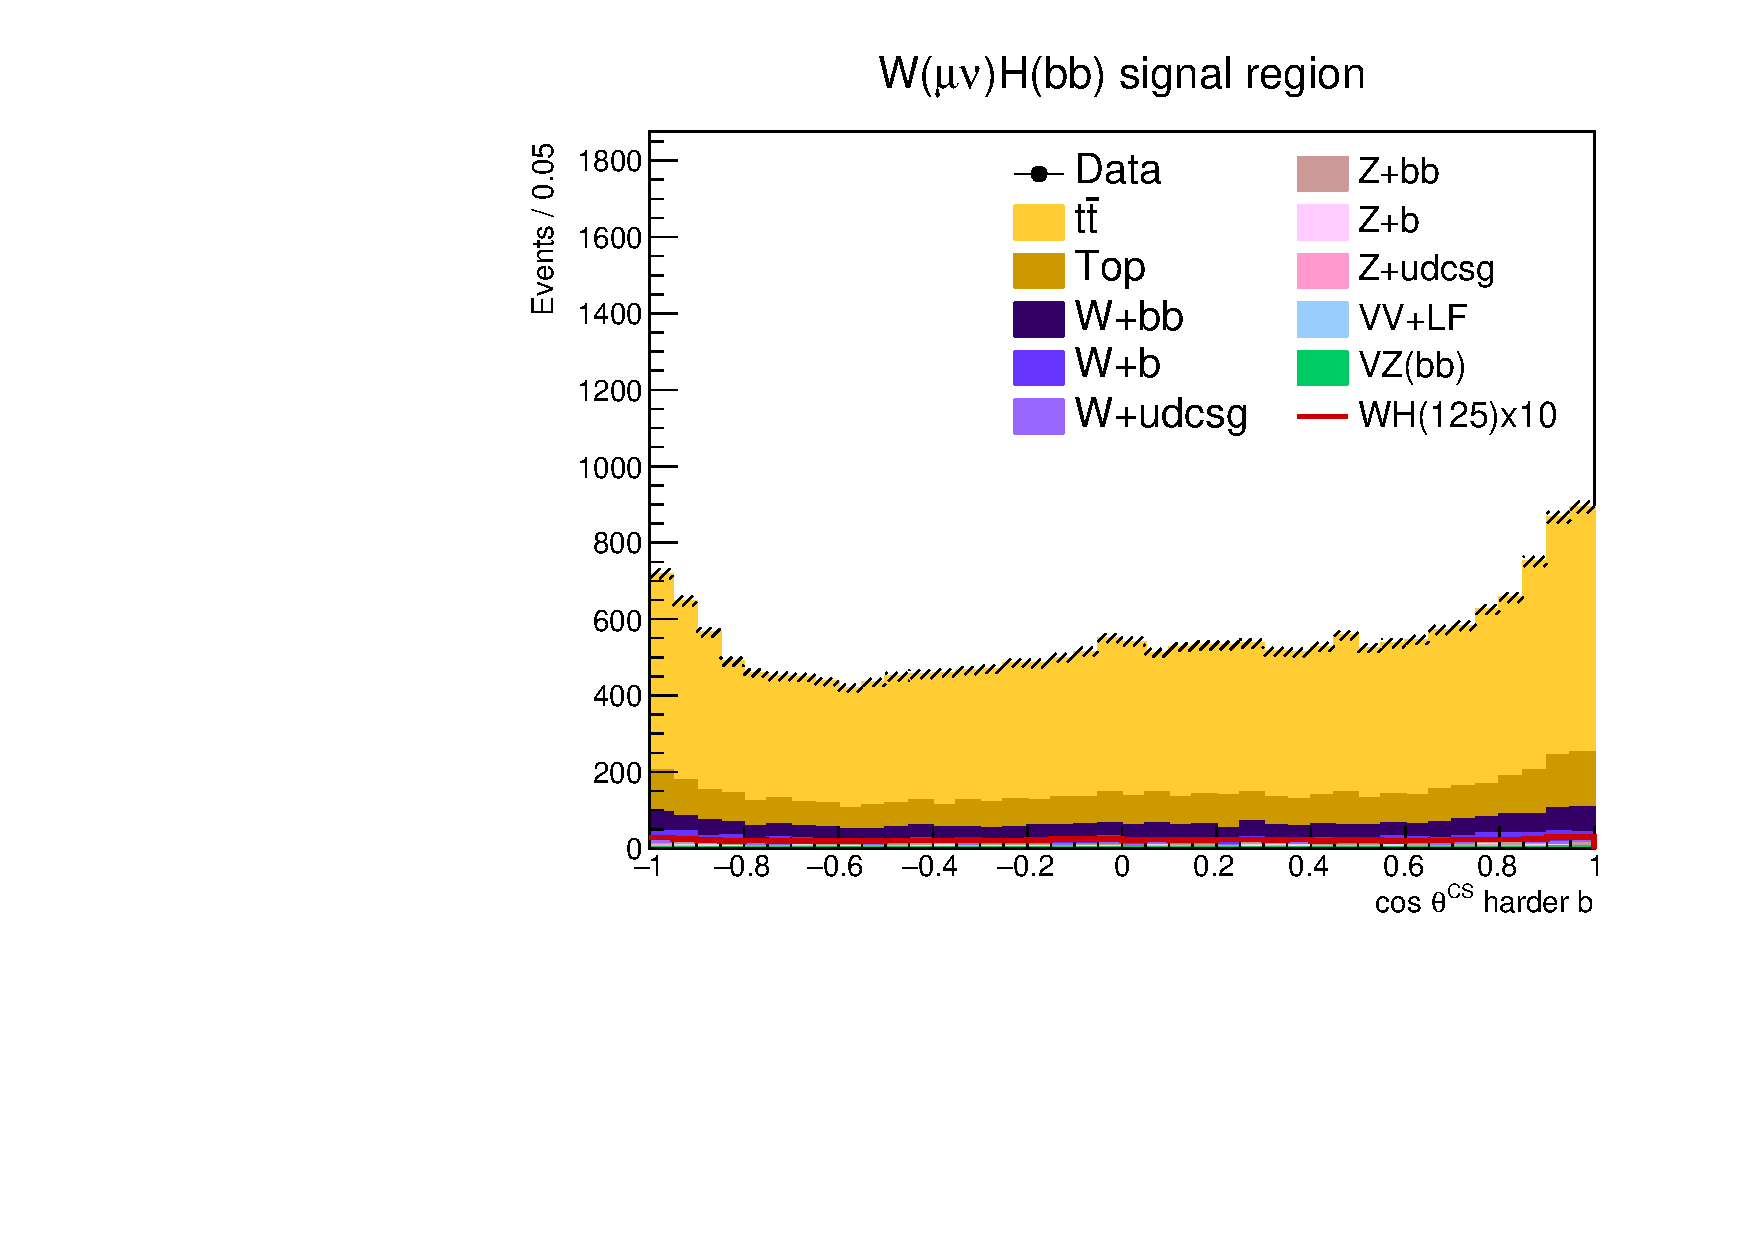
\includegraphics[width=0.48\textwidth]{figures/wlnhbb2016/resolved/WmnWHSR_hbbCosThetaCSJ1.pdf}
    \caption{\HBB\ reconstruction in the resolved category W($\mu\nu$) signal region.
    Left to right and top to bottom: higher b-tagged jet $\pt$, lower b-tagged jet $\pt$, dijet mass, dijet $\pt$, 
    pseudorapidity difference between the two jets, and the Collins-Soper angle of the harder b-tagged jet.
    The simulated shapes are prefit, with the postfit normalizations applied.}
    \label{fig:res_WmnSR_Hbb}
  \end{center}
\end{figure}
\clearpage

\begin{figure}[tbp]
  \begin{center}
    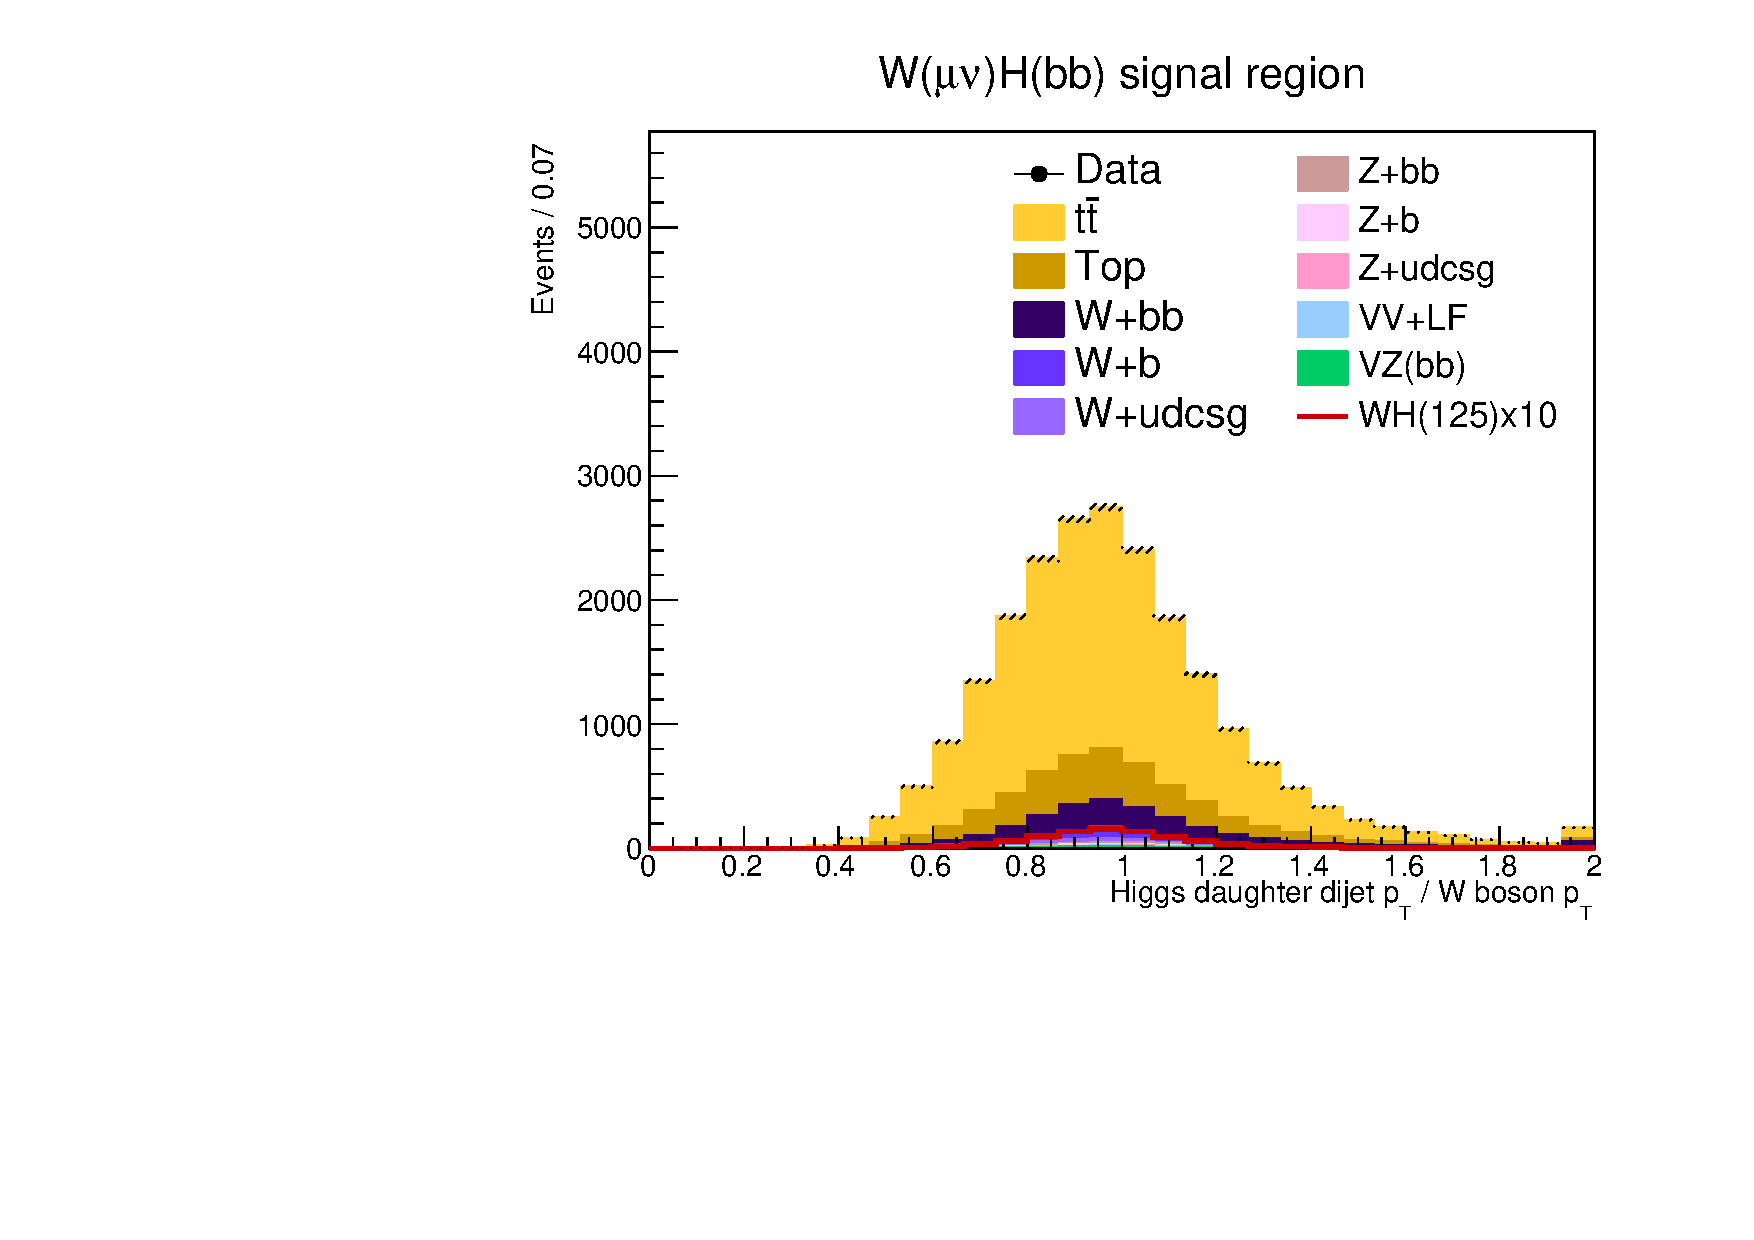
\includegraphics[width=0.48\textwidth]{figures/wlnhbb2016/resolved/WmnWHSR_pTBalanceDijetW.pdf}
    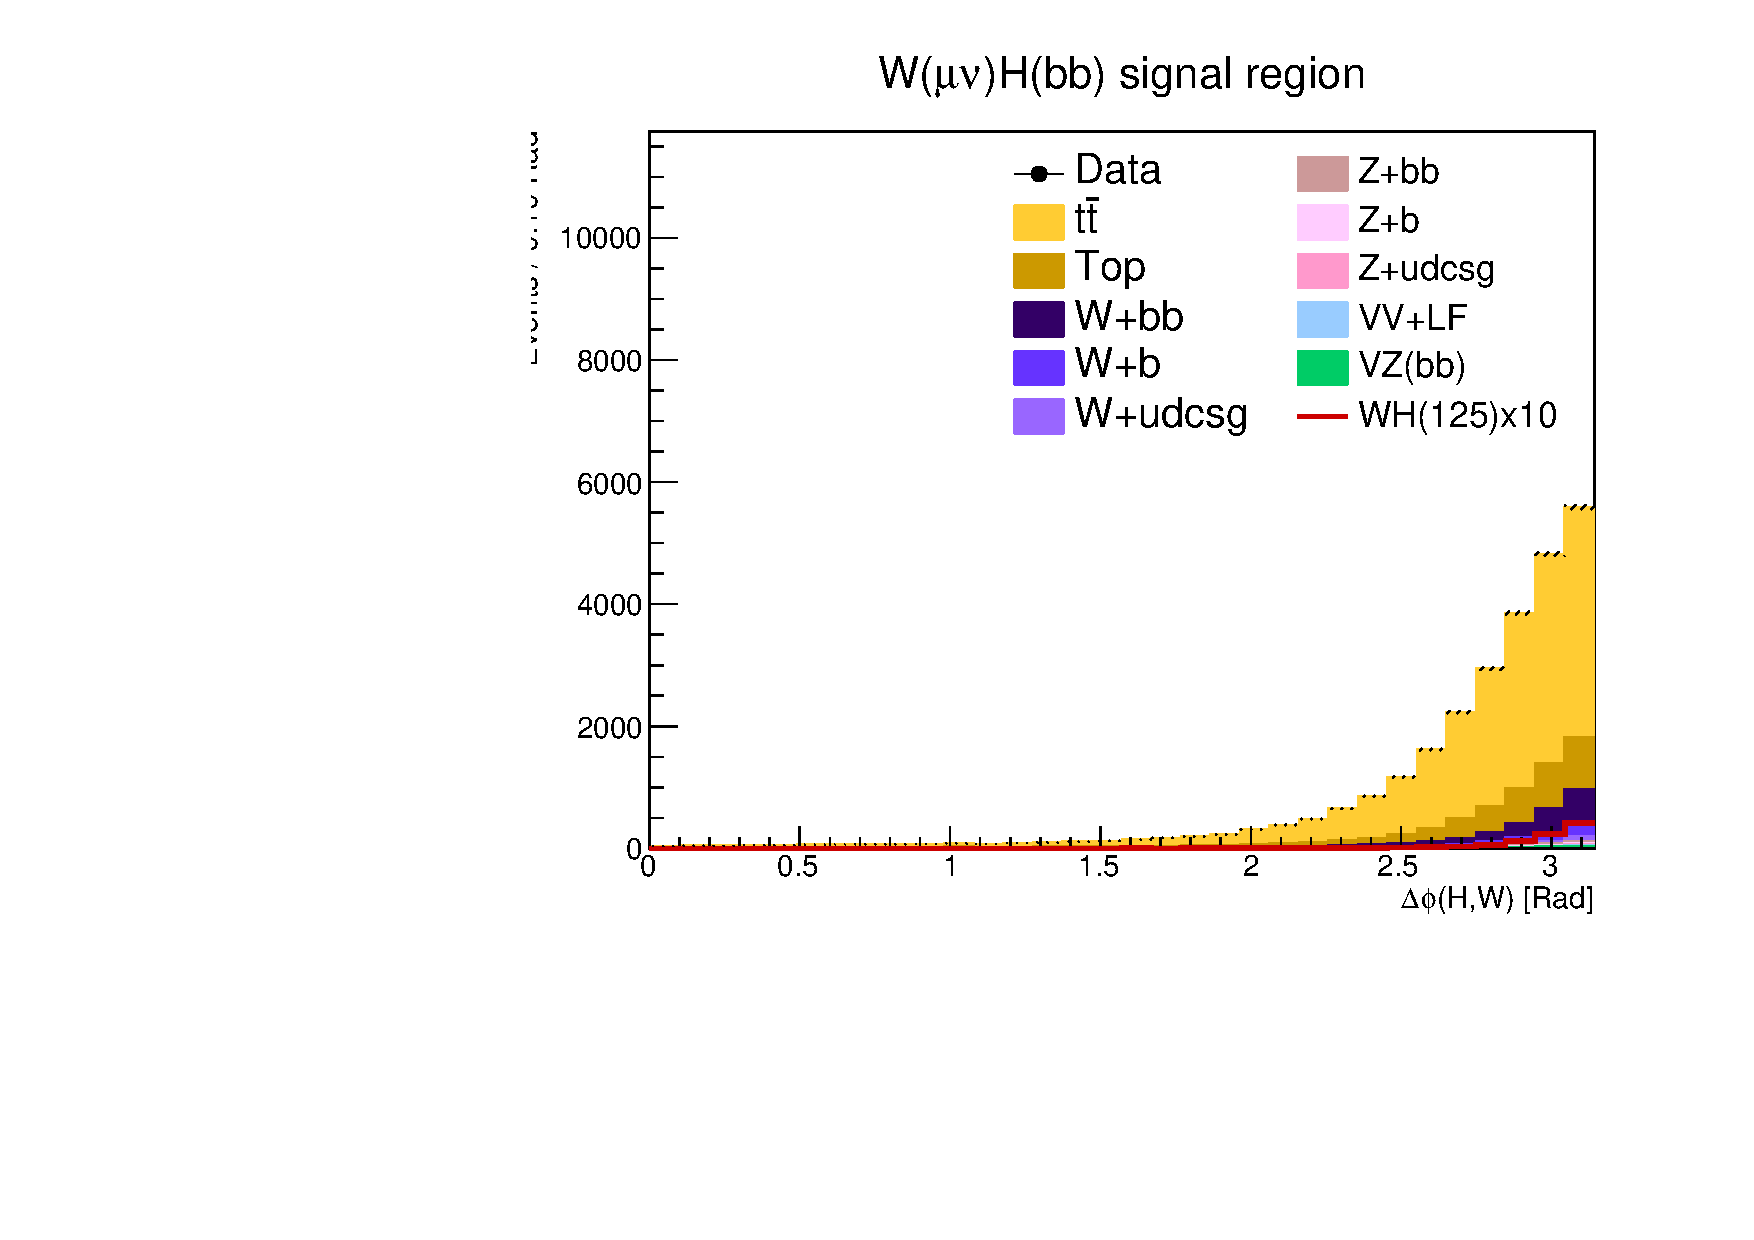
\includegraphics[width=0.48\textwidth]{figures/wlnhbb2016/resolved/WmnWHSR_deltaPhiVH.pdf}
    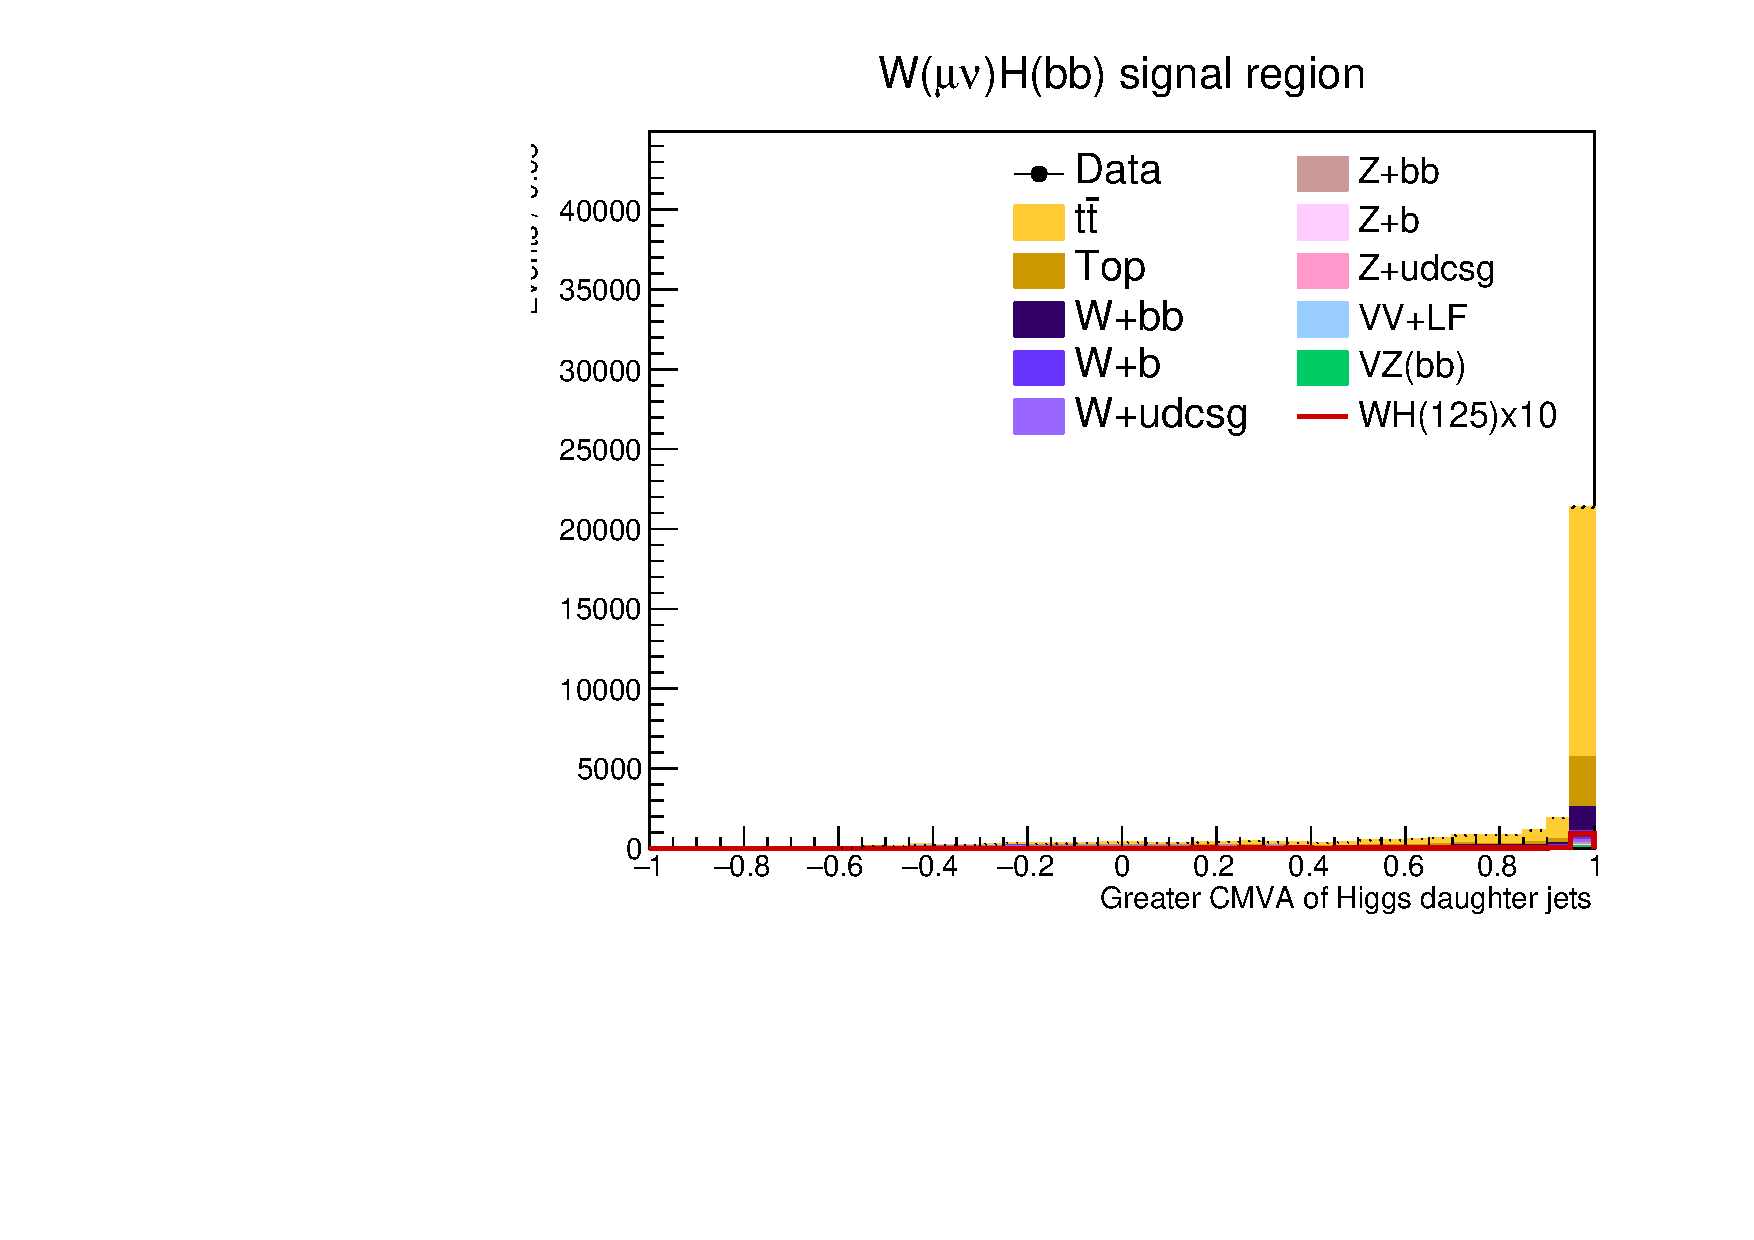
\includegraphics[width=0.48\textwidth]{figures/wlnhbb2016/resolved/WmnWHSR_bDiscrMax.pdf}
    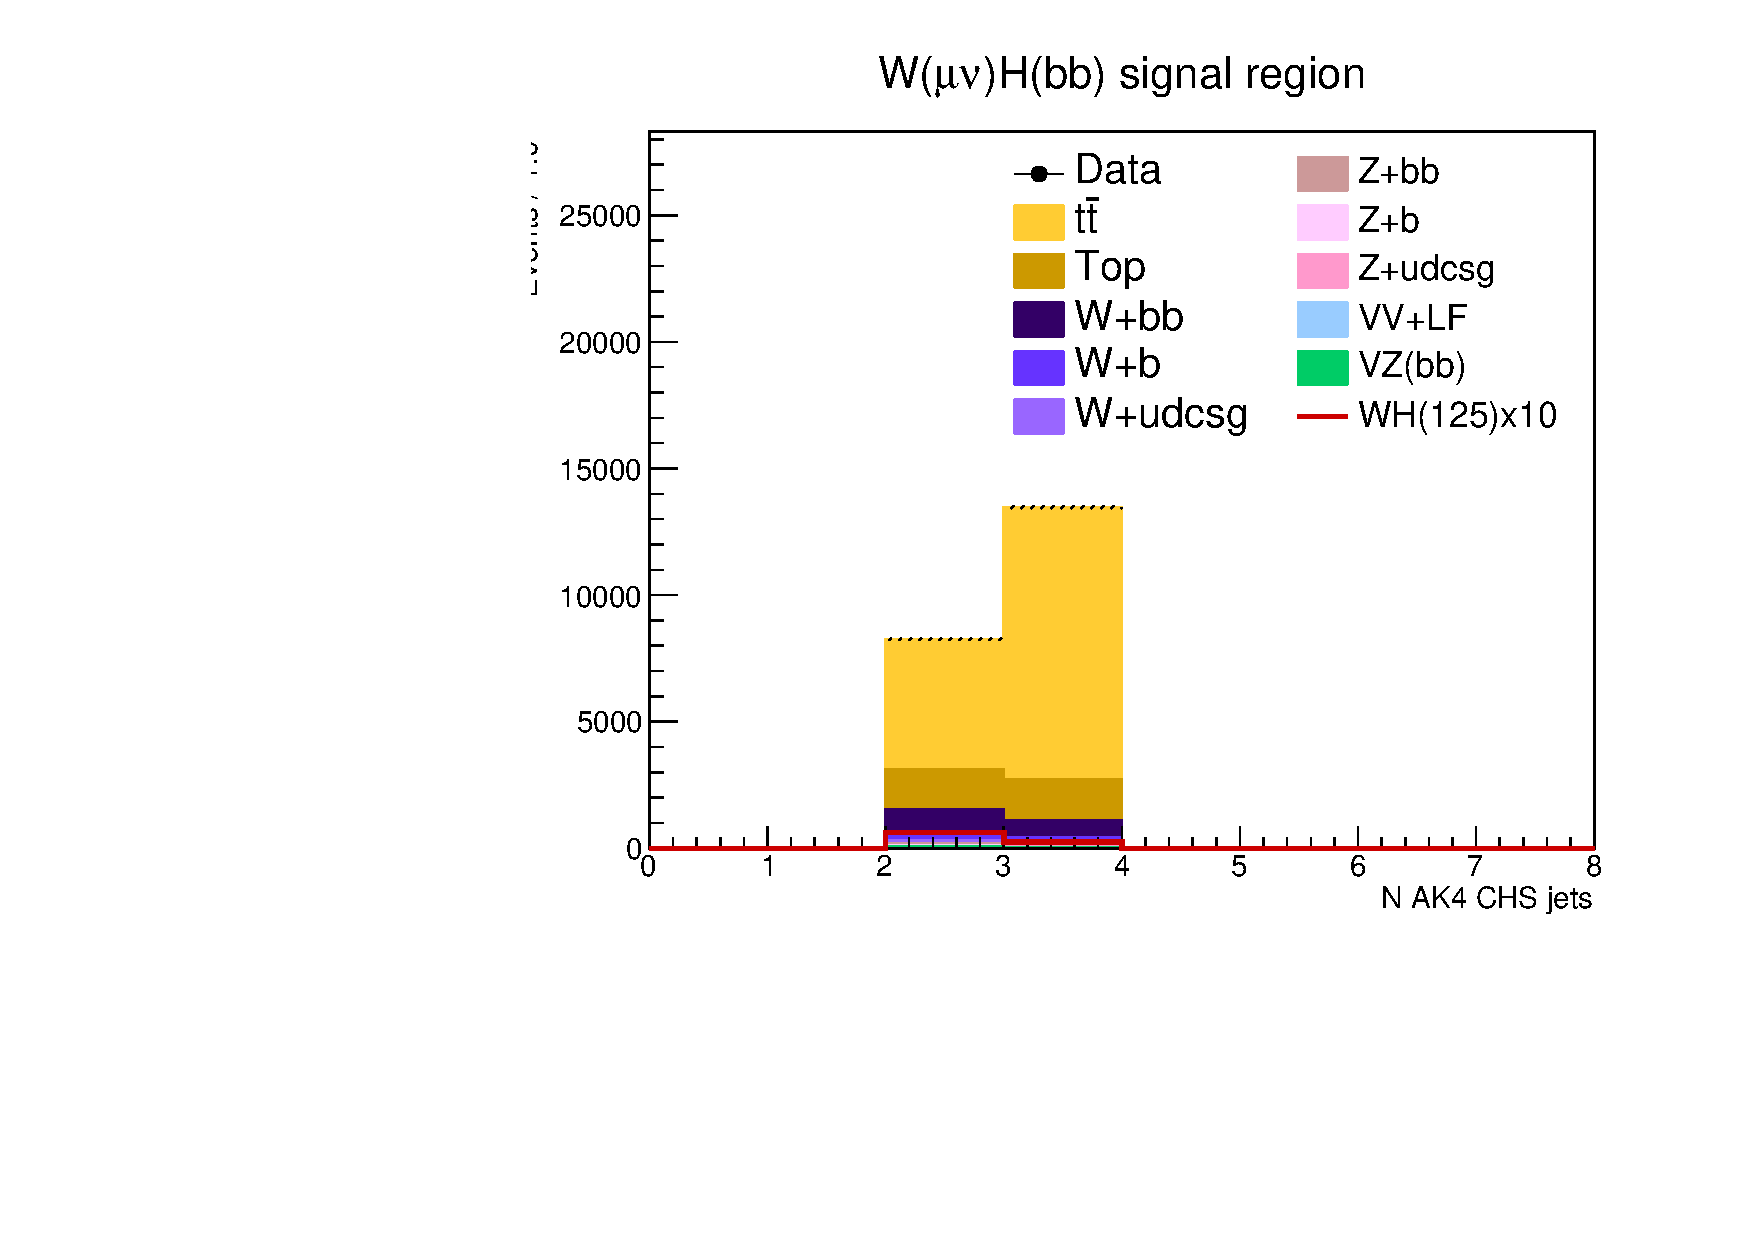
\includegraphics[width=0.48\textwidth]{figures/wlnhbb2016/resolved/WmnWHSR_nJet.pdf}
    \includegraphics[width=0.48\textwidth]{figures/wlnhbb2016/resolved/WmnWHSR_nSoft5.pdf}
    \includegraphics[width=0.48\textwidth]{figures/wlnhbb2016/resolved/WmnWHSR_bdtValue.pdf}
    \caption{WH kinematics in the resolved category W($\mu\nu$) signal region.
    Left to right and top to bottom: WH $\pt$ balance, WH azimuthal separation, leading b-tag score, the number of central jets,
    the number of 5 \GeV\ soft activity jets, and the evaluation of the signal extraction BDT.
    The simulated shapes are prefit, with the postfit normalizations applied.}
    \label{fig:res_WmnSR_WH}
  \end{center}
\end{figure}
\clearpage

\begin{figure}[tbp]
  \begin{center}
    \includegraphics[width=0.48\textwidth]{figures/wlnhbb2016/resolved/WenWHLightFlavorCR_lepton1Pt.pdf}
    \includegraphics[width=0.48\textwidth]{figures/wlnhbb2016/resolved/WenWHLightFlavorCR_pfmet.pdf}
    \includegraphics[width=0.48\textwidth]{figures/wlnhbb2016/resolved/WenWHLightFlavorCR_WpT.pdf}
    \includegraphics[width=0.48\textwidth]{figures/wlnhbb2016/resolved/WenWHLightFlavorCR_mTW.pdf}
    \includegraphics[width=0.48\textwidth]{figures/wlnhbb2016/resolved/WenWHLightFlavorCR_topMassLep1Met.pdf}
    \includegraphics[width=0.48\textwidth]{figures/wlnhbb2016/resolved/WenWHLightFlavorCR_pfmetsig.pdf}
    \caption{W boson reconstruction in the resolved category W(e$\nu$)+LF control region.
    Left to right and top to bottom: electron $\pt$, $\MET$, W boson $\pt$, W boson transverse mass,
    the reconstructed top quark mass, and the $\MET$ significance.
    The simulated shapes are prefit, with the postfit normalizations applied.}
    \label{fig:res_WenLF_WBosons}
  \end{center}
\end{figure}
\clearpage

\begin{figure}[tbp]
  \begin{center}
    \includegraphics[width=0.48\textwidth]{figures/wlnhbb2016/resolved/WenWHLightFlavorCR_Hbjet1Pt.pdf}
    \includegraphics[width=0.48\textwidth]{figures/wlnhbb2016/resolved/WenWHLightFlavorCR_Hbjet2Pt.pdf}
    \includegraphics[width=0.48\textwidth]{figures/wlnhbb2016/resolved/WenWHLightFlavorCR_mH.pdf}
    \includegraphics[width=0.48\textwidth]{figures/wlnhbb2016/resolved/WenWHLightFlavorCR_pTH.pdf}
    \includegraphics[width=0.48\textwidth]{figures/wlnhbb2016/resolved/WenWHLightFlavorCR_dEtab1b2.pdf}
    \includegraphics[width=0.48\textwidth]{figures/wlnhbb2016/resolved/WenWHLightFlavorCR_hbbCosThetaCSJ1.pdf}
    \caption{\HBB\ reconstruction in the resolved category W(e$\nu$)+LF control region.
    Left to right and top to bottom: higher b-tagged jet $\pt$, lower b-tagged jet $\pt$, dijet mass, dijet $\pt$, 
    pseudorapidity difference between the two jets, and the Collins-Soper angle of the harder b-tagged jet.
    The simulated shapes are prefit, with the postfit normalizations applied.}
    \label{fig:res_WenLF_Hbb}
  \end{center}
\end{figure}
\clearpage

\begin{figure}[tbp]
  \begin{center}
    \includegraphics[width=0.48\textwidth]{figures/wlnhbb2016/resolved/WenWHLightFlavorCR_pTBalanceDijetW.pdf}
    \includegraphics[width=0.48\textwidth]{figures/wlnhbb2016/resolved/WenWHLightFlavorCR_deltaPhiVH.pdf}
    \includegraphics[width=0.48\textwidth]{figures/wlnhbb2016/resolved/WenWHLightFlavorCR_bDiscrMax.pdf}
    \includegraphics[width=0.48\textwidth]{figures/wlnhbb2016/resolved/WenWHLightFlavorCR_nJet.pdf}
    \includegraphics[width=0.48\textwidth]{figures/wlnhbb2016/resolved/WenWHLightFlavorCR_nSoft5.pdf}
    \includegraphics[width=0.48\textwidth]{figures/wlnhbb2016/resolved/WenWHLightFlavorCR_bdtValue.pdf}
    \caption{WH kinematics in the resolved category W(e$\nu$)+LF control region.
    Left to right and top to bottom: WH $\pt$ balance, WH azimuthal separation, leading b-tag score, the number of central jets,
    the number of 5 \GeV\ soft activity jets, and the evaluation of the signal extraction BDT.
    The simulated shapes are prefit, with the postfit normalizations applied.}
    \label{fig:res_WenLF_WH}
  \end{center}
\end{figure}
\clearpage


\begin{figure}[tbp]
  \begin{center}
    \includegraphics[width=0.48\textwidth]{figures/wlnhbb2016/resolved/WmnWHLightFlavorCR_lepton1Pt.pdf}
    \includegraphics[width=0.48\textwidth]{figures/wlnhbb2016/resolved/WmnWHLightFlavorCR_pfmet.pdf}
    \includegraphics[width=0.48\textwidth]{figures/wlnhbb2016/resolved/WmnWHLightFlavorCR_WpT.pdf}
    \includegraphics[width=0.48\textwidth]{figures/wlnhbb2016/resolved/WmnWHLightFlavorCR_mTW.pdf}
    \includegraphics[width=0.48\textwidth]{figures/wlnhbb2016/resolved/WmnWHLightFlavorCR_topMassLep1Met.pdf}
    \includegraphics[width=0.48\textwidth]{figures/wlnhbb2016/resolved/WmnWHLightFlavorCR_pfmetsig.pdf}
    \caption{W boson reconstruction in the resolved category W($\mu\nu$)+LF control region.
    Left to right and top to bottom: muon $\pt$, $\MET$, W boson $\pt$, W boson transverse mass,
    the reconstructed top quark mass, and the $\MET$ significance.
    The simulated shapes are prefit, with the postfit normalizations applied.}
    \label{fig:res_WmnLF_WBosons}
  \end{center}
\end{figure}
\clearpage

\begin{figure}[tbp]
  \begin{center}
    \includegraphics[width=0.48\textwidth]{figures/wlnhbb2016/resolved/WmnWHLightFlavorCR_Hbjet1Pt.pdf}
    \includegraphics[width=0.48\textwidth]{figures/wlnhbb2016/resolved/WmnWHLightFlavorCR_Hbjet2Pt.pdf}
    \includegraphics[width=0.48\textwidth]{figures/wlnhbb2016/resolved/WmnWHLightFlavorCR_mH.pdf}
    \includegraphics[width=0.48\textwidth]{figures/wlnhbb2016/resolved/WmnWHLightFlavorCR_pTH.pdf}
    \includegraphics[width=0.48\textwidth]{figures/wlnhbb2016/resolved/WmnWHLightFlavorCR_dEtab1b2.pdf}
    \includegraphics[width=0.48\textwidth]{figures/wlnhbb2016/resolved/WmnWHLightFlavorCR_hbbCosThetaCSJ1.pdf}
    \caption{\HBB\ reconstruction in the resolved category W($\mu\nu$)+LF control region.
    Left to right and top to bottom: higher b-tagged jet $\pt$, lower b-tagged jet $\pt$, dijet mass, dijet $\pt$, 
    pseudorapidity difference between the two jets, and the Collins-Soper angle of the harder b-tagged jet.
    The simulated shapes are prefit, with the postfit normalizations applied.}
    \label{fig:res_WmnLF_Hbb}
  \end{center}
\end{figure}
\clearpage

\begin{figure}[tbp]
  \begin{center}
    \includegraphics[width=0.48\textwidth]{figures/wlnhbb2016/resolved/WmnWHLightFlavorCR_pTBalanceDijetW.pdf}
    \includegraphics[width=0.48\textwidth]{figures/wlnhbb2016/resolved/WmnWHLightFlavorCR_deltaPhiVH.pdf}
    \includegraphics[width=0.48\textwidth]{figures/wlnhbb2016/resolved/WmnWHLightFlavorCR_bDiscrMax.pdf}
    \includegraphics[width=0.48\textwidth]{figures/wlnhbb2016/resolved/WmnWHLightFlavorCR_nJet.pdf}
    \includegraphics[width=0.48\textwidth]{figures/wlnhbb2016/resolved/WmnWHLightFlavorCR_nSoft5.pdf}
    \includegraphics[width=0.48\textwidth]{figures/wlnhbb2016/resolved/WmnWHLightFlavorCR_bdtValue.pdf}
    \caption{WH kinematics in the resolved category W($\mu\nu$)+LF control region.
    Left to right and top to bottom: WH $\pt$ balance, WH azimuthal separation, leading b-tag score, the number of central jets,
    the number of 5 \GeV\ soft activity jets, and the evaluation of the signal extraction BDT.
    The simulated shapes are prefit, with the postfit normalizations applied.}
    \label{fig:res_WmnLF_WH}
  \end{center}
\end{figure}
\clearpage


\begin{figure}[tbp]
  \begin{center}
    \includegraphics[width=0.48\textwidth]{figures/wlnhbb2016/resolved/WenWH2TopCR_lepton1Pt.pdf}
    \includegraphics[width=0.48\textwidth]{figures/wlnhbb2016/resolved/WenWH2TopCR_pfmet.pdf}
    \includegraphics[width=0.48\textwidth]{figures/wlnhbb2016/resolved/WenWH2TopCR_WpT.pdf}
    \includegraphics[width=0.48\textwidth]{figures/wlnhbb2016/resolved/WenWH2TopCR_mTW.pdf}
    \includegraphics[width=0.48\textwidth]{figures/wlnhbb2016/resolved/WenWH2TopCR_topMassLep1Met.pdf}
    \includegraphics[width=0.48\textwidth]{figures/wlnhbb2016/resolved/WenWH2TopCR_pfmetsig.pdf}
    \caption{W boson reconstruction in the resolved category W(e$\nu$) \ttbar control region.
    Left to right and top to bottom: electron $\pt$, $\MET$, W boson $\pt$, W boson transverse mass,
    the reconstructed top quark mass, and the $\MET$ significance.
    The simulated shapes are prefit, with the postfit normalizations applied.}
    \label{fig:res_WenTT_WBosons}
  \end{center}
\end{figure}
\clearpage

\begin{figure}[tbp]
  \begin{center}
    \includegraphics[width=0.48\textwidth]{figures/wlnhbb2016/resolved/WenWH2TopCR_Hbjet1Pt.pdf}
    \includegraphics[width=0.48\textwidth]{figures/wlnhbb2016/resolved/WenWH2TopCR_Hbjet2Pt.pdf}
    \includegraphics[width=0.48\textwidth]{figures/wlnhbb2016/resolved/WenWH2TopCR_mH.pdf}
    \includegraphics[width=0.48\textwidth]{figures/wlnhbb2016/resolved/WenWH2TopCR_pTH.pdf}
    \includegraphics[width=0.48\textwidth]{figures/wlnhbb2016/resolved/WenWH2TopCR_dEtab1b2.pdf}
    \includegraphics[width=0.48\textwidth]{figures/wlnhbb2016/resolved/WenWH2TopCR_hbbCosThetaCSJ1.pdf}
    \caption{\HBB\ reconstruction in the resolved category W(e$\nu$) \ttbar control region.
    Left to right and top to bottom: higher b-tagged jet $\pt$, lower b-tagged jet $\pt$, dijet mass, dijet $\pt$, 
    pseudorapidity difference between the two jets, and the Collins-Soper angle of the harder b-tagged jet.
    The simulated shapes are prefit, with the postfit normalizations applied.}
    \label{fig:res_WenTT_Hbb}
  \end{center}
\end{figure}
\clearpage

\begin{figure}[tbp]
  \begin{center}
    \includegraphics[width=0.48\textwidth]{figures/wlnhbb2016/resolved/WenWH2TopCR_pTBalanceDijetW.pdf}
    \includegraphics[width=0.48\textwidth]{figures/wlnhbb2016/resolved/WenWH2TopCR_deltaPhiVH.pdf}
    \includegraphics[width=0.48\textwidth]{figures/wlnhbb2016/resolved/WenWH2TopCR_bDiscrMax.pdf}
    \includegraphics[width=0.48\textwidth]{figures/wlnhbb2016/resolved/WenWH2TopCR_nJet.pdf}
    \includegraphics[width=0.48\textwidth]{figures/wlnhbb2016/resolved/WenWH2TopCR_nSoft5.pdf}
    \includegraphics[width=0.48\textwidth]{figures/wlnhbb2016/resolved/WenWH2TopCR_bdtValue.pdf}
    \caption{WH kinematics in the resolved category W(e$\nu$) \ttbar control region.
    Left to right and top to bottom: WH $\pt$ balance, WH azimuthal separation, leading b-tag score, the number of central jets,
    the number of 5 \GeV\ soft activity jets, and the evaluation of the signal extraction BDT.
    The simulated shapes are prefit, with the postfit normalizations applied.}
    \label{fig:res_WenTT_WH}
  \end{center}
\end{figure}
\clearpage


\begin{figure}[tbp]
  \begin{center}
    \includegraphics[width=0.48\textwidth]{figures/wlnhbb2016/resolved/WmnWH2TopCR_lepton1Pt.pdf}
    \includegraphics[width=0.48\textwidth]{figures/wlnhbb2016/resolved/WmnWH2TopCR_pfmet.pdf}
    \includegraphics[width=0.48\textwidth]{figures/wlnhbb2016/resolved/WmnWH2TopCR_WpT.pdf}
    \includegraphics[width=0.48\textwidth]{figures/wlnhbb2016/resolved/WmnWH2TopCR_mTW.pdf}
    \includegraphics[width=0.48\textwidth]{figures/wlnhbb2016/resolved/WmnWH2TopCR_topMassLep1Met.pdf}
    \includegraphics[width=0.48\textwidth]{figures/wlnhbb2016/resolved/WmnWH2TopCR_pfmetsig.pdf}
    \caption{W boson reconstruction in the resolved category W($\mu\nu$) \ttbar control region.
    Left to right and top to bottom: muon $\pt$, $\MET$, W boson $\pt$, W boson transverse mass,
    the reconstructed top quark mass, and the $\MET$ significance.
    The simulated shapes are prefit, with the postfit normalizations applied.}
    \label{fig:res_WmnTT_WBosons}
  \end{center}
\end{figure}
\clearpage

\begin{figure}[tbp]
  \begin{center}
    \includegraphics[width=0.48\textwidth]{figures/wlnhbb2016/resolved/WmnWH2TopCR_Hbjet1Pt.pdf}
    \includegraphics[width=0.48\textwidth]{figures/wlnhbb2016/resolved/WmnWH2TopCR_Hbjet2Pt.pdf}
    \includegraphics[width=0.48\textwidth]{figures/wlnhbb2016/resolved/WmnWH2TopCR_mH.pdf}
    \includegraphics[width=0.48\textwidth]{figures/wlnhbb2016/resolved/WmnWH2TopCR_pTH.pdf}
    \includegraphics[width=0.48\textwidth]{figures/wlnhbb2016/resolved/WmnWH2TopCR_dEtab1b2.pdf}
    \includegraphics[width=0.48\textwidth]{figures/wlnhbb2016/resolved/WmnWH2TopCR_hbbCosThetaCSJ1.pdf}
    \caption{\HBB\ reconstruction in the resolved category W($\mu\nu$) \ttbar control region.
    Left to right and top to bottom: higher b-tagged jet $\pt$, lower b-tagged jet $\pt$, dijet mass, dijet $\pt$, 
    pseudorapidity difference between the two jets, and the Collins-Soper angle of the harder b-tagged jet.
    The simulated shapes are prefit, with the postfit normalizations applied.}
    \label{fig:res_WmnTT_Hbb}
  \end{center}
\end{figure}
\clearpage

\begin{figure}[tbp]
  \begin{center}
    \includegraphics[width=0.48\textwidth]{figures/wlnhbb2016/resolved/WmnWH2TopCR_pTBalanceDijetW.pdf}
    \includegraphics[width=0.48\textwidth]{figures/wlnhbb2016/resolved/WmnWH2TopCR_deltaPhiVH.pdf}
    \includegraphics[width=0.48\textwidth]{figures/wlnhbb2016/resolved/WmnWH2TopCR_bDiscrMax.pdf}
    \includegraphics[width=0.48\textwidth]{figures/wlnhbb2016/resolved/WmnWH2TopCR_nJet.pdf}
    \includegraphics[width=0.48\textwidth]{figures/wlnhbb2016/resolved/WmnWH2TopCR_nSoft5.pdf}
    \includegraphics[width=0.48\textwidth]{figures/wlnhbb2016/resolved/WmnWH2TopCR_bdtValue.pdf}
    \caption{WH kinematics in the resolved category W($\mu\nu$) \ttbar control region.
    Left to right and top to bottom: WH $\pt$ balance, WH azimuthal separation, leading b-tag score, the number of central jets,
    the number of 5 \GeV\ soft activity jets, and the evaluation of the signal extraction BDT.
    The simulated shapes are prefit, with the postfit normalizations applied.}
    \label{fig:res_WmnTT_WH}
  \end{center}
\end{figure}
\clearpage

\begin{figure}[tbp]
  \begin{center}
    \includegraphics[width=0.48\textwidth]{figures/wlnhbb2016/resolved/WenWHHeavyFlavorCRLowMass_lepton1Pt.pdf}
    \includegraphics[width=0.48\textwidth]{figures/wlnhbb2016/resolved/WenWHHeavyFlavorCRLowMass_pfmet.pdf}
    \includegraphics[width=0.48\textwidth]{figures/wlnhbb2016/resolved/WenWHHeavyFlavorCRLowMass_WpT.pdf}
    \includegraphics[width=0.48\textwidth]{figures/wlnhbb2016/resolved/WenWHHeavyFlavorCRLowMass_mTW.pdf}
    \includegraphics[width=0.48\textwidth]{figures/wlnhbb2016/resolved/WenWHHeavyFlavorCRLowMass_topMassLep1Met.pdf}
    \includegraphics[width=0.48\textwidth]{figures/wlnhbb2016/resolved/WenWHHeavyFlavorCRLowMass_pfmetsig.pdf}
    \caption{W boson reconstruction in the resolved category W(e$\nu$)+HF low mass control region.
    Left to right and top to bottom: electron $\pt$, $\MET$, W boson $\pt$, W boson transverse mass,
    the reconstructed top quark mass, and the $\MET$ significance.
    The simulated shapes are prefit, with the postfit normalizations applied.}
    \label{fig:res_WenHFLowMass_WBosons}
  \end{center}
\end{figure}
\clearpage

\begin{figure}[tbp]
  \begin{center}
    \includegraphics[width=0.48\textwidth]{figures/wlnhbb2016/resolved/WenWHHeavyFlavorCRLowMass_Hbjet1Pt.pdf}
    \includegraphics[width=0.48\textwidth]{figures/wlnhbb2016/resolved/WenWHHeavyFlavorCRLowMass_Hbjet2Pt.pdf}
    \includegraphics[width=0.48\textwidth]{figures/wlnhbb2016/resolved/WenWHHeavyFlavorCRLowMass_mH.pdf}
    \includegraphics[width=0.48\textwidth]{figures/wlnhbb2016/resolved/WenWHHeavyFlavorCRLowMass_pTH.pdf}
    \includegraphics[width=0.48\textwidth]{figures/wlnhbb2016/resolved/WenWHHeavyFlavorCRLowMass_dEtab1b2.pdf}
    \includegraphics[width=0.48\textwidth]{figures/wlnhbb2016/resolved/WenWHHeavyFlavorCRLowMass_hbbCosThetaCSJ1.pdf}
    \caption{\HBB\ reconstruction in the resolved category W(e$\nu$)+HF low mass control region.
    Left to right and top to bottom: higher b-tagged jet $\pt$, lower b-tagged jet $\pt$, dijet mass, dijet $\pt$, 
    pseudorapidity difference between the two jets, and the Collins-Soper angle of the harder b-tagged jet.
    The simulated shapes are prefit, with the postfit normalizations applied.}
    \label{fig:res_WenHFLowMass_Hbb}
  \end{center}
\end{figure}
\clearpage

\begin{figure}[tbp]
  \begin{center}
    \includegraphics[width=0.48\textwidth]{figures/wlnhbb2016/resolved/WenWHHeavyFlavorCRLowMass_pTBalanceDijetW.pdf}
    \includegraphics[width=0.48\textwidth]{figures/wlnhbb2016/resolved/WenWHHeavyFlavorCRLowMass_deltaPhiVH.pdf}
    \includegraphics[width=0.48\textwidth]{figures/wlnhbb2016/resolved/WenWHHeavyFlavorCRLowMass_bDiscrMax.pdf}
    \includegraphics[width=0.48\textwidth]{figures/wlnhbb2016/resolved/WenWHHeavyFlavorCRLowMass_nJet.pdf}
    \includegraphics[width=0.48\textwidth]{figures/wlnhbb2016/resolved/WenWHHeavyFlavorCRLowMass_nSoft5.pdf}
    \includegraphics[width=0.48\textwidth]{figures/wlnhbb2016/resolved/WenWHHeavyFlavorCRLowMass_bdtValue.pdf}
    \caption{WH kinematics in the resolved category W(e$\nu$)+HF low mass control region.
    Left to right and top to bottom: WH $\pt$ balance, WH azimuthal separation, leading b-tag score, the number of central jets,
    the number of 5 \GeV\ soft activity jets, and the evaluation of the signal extraction BDT.
    The simulated shapes are prefit, with the postfit normalizations applied.}
    \label{fig:res_WenHFLowMass_WH}
  \end{center}
\end{figure}
\clearpage


\begin{figure}[tbp]
  \begin{center}
    \includegraphics[width=0.48\textwidth]{figures/wlnhbb2016/resolved/WmnWHHeavyFlavorCRLowMass_lepton1Pt.pdf}
    \includegraphics[width=0.48\textwidth]{figures/wlnhbb2016/resolved/WmnWHHeavyFlavorCRLowMass_pfmet.pdf}
    \includegraphics[width=0.48\textwidth]{figures/wlnhbb2016/resolved/WmnWHHeavyFlavorCRLowMass_WpT.pdf}
    \includegraphics[width=0.48\textwidth]{figures/wlnhbb2016/resolved/WmnWHHeavyFlavorCRLowMass_mTW.pdf}
    \includegraphics[width=0.48\textwidth]{figures/wlnhbb2016/resolved/WmnWHHeavyFlavorCRLowMass_topMassLep1Met.pdf}
    \includegraphics[width=0.48\textwidth]{figures/wlnhbb2016/resolved/WmnWHHeavyFlavorCRLowMass_pfmetsig.pdf}
    \caption{W boson reconstruction in the resolved category W($\mu\nu$)+HF low mass control region.
    Left to right and top to bottom: muon $\pt$, $\MET$, W boson $\pt$, W boson transverse mass,
    the reconstructed top quark mass, and the $\MET$ significance.
    The simulated shapes are prefit, with the postfit normalizations applied.}
    \label{fig:res_WmnHFLowMass_WBosons}
  \end{center}
\end{figure}
\clearpage

\begin{figure}[tbp]
  \begin{center}
    \includegraphics[width=0.48\textwidth]{figures/wlnhbb2016/resolved/WmnWHHeavyFlavorCRLowMass_Hbjet1Pt.pdf}
    \includegraphics[width=0.48\textwidth]{figures/wlnhbb2016/resolved/WmnWHHeavyFlavorCRLowMass_Hbjet2Pt.pdf}
    \includegraphics[width=0.48\textwidth]{figures/wlnhbb2016/resolved/WmnWHHeavyFlavorCRLowMass_mH.pdf}
    \includegraphics[width=0.48\textwidth]{figures/wlnhbb2016/resolved/WmnWHHeavyFlavorCRLowMass_pTH.pdf}
    \includegraphics[width=0.48\textwidth]{figures/wlnhbb2016/resolved/WmnWHHeavyFlavorCRLowMass_dEtab1b2.pdf}
    \includegraphics[width=0.48\textwidth]{figures/wlnhbb2016/resolved/WmnWHHeavyFlavorCRLowMass_hbbCosThetaCSJ1.pdf}
    \caption{\HBB\ reconstruction in the resolved category W($\mu\nu$)+HF low mass control region.
    Left to right and top to bottom: higher b-tagged jet $\pt$, lower b-tagged jet $\pt$, dijet mass, dijet $\pt$, 
    pseudorapidity difference between the two jets, and the Collins-Soper angle of the harder b-tagged jet.
    The simulated shapes are prefit, with the postfit normalizations applied.}
    \label{fig:res_WmnHFLowMass_Hbb}
  \end{center}
\end{figure}
\clearpage

\begin{figure}[tbp]
  \begin{center}
    \includegraphics[width=0.48\textwidth]{figures/wlnhbb2016/resolved/WmnWHHeavyFlavorCRLowMass_pTBalanceDijetW.pdf}
    \includegraphics[width=0.48\textwidth]{figures/wlnhbb2016/resolved/WmnWHHeavyFlavorCRLowMass_deltaPhiVH.pdf}
    \includegraphics[width=0.48\textwidth]{figures/wlnhbb2016/resolved/WmnWHHeavyFlavorCRLowMass_bDiscrMax.pdf}
    \includegraphics[width=0.48\textwidth]{figures/wlnhbb2016/resolved/WmnWHHeavyFlavorCRLowMass_nJet.pdf}
    \includegraphics[width=0.48\textwidth]{figures/wlnhbb2016/resolved/WmnWHHeavyFlavorCRLowMass_nSoft5.pdf}
    \includegraphics[width=0.48\textwidth]{figures/wlnhbb2016/resolved/WmnWHHeavyFlavorCRLowMass_bdtValue.pdf}
    \caption{WH kinematics in the resolved category W($\mu\nu$)+HF low mass control region.
    Left to right and top to bottom: WH $\pt$ balance, WH azimuthal separation, leading b-tag score, the number of central jets,
    the number of 5 \GeV\ soft activity jets, and the evaluation of the signal extraction BDT.
    The simulated shapes are prefit, with the postfit normalizations applied.}
    \label{fig:res_WmnHFLowMass_WH}
  \end{center}
\end{figure}
\clearpage

\begin{figure}[tbp]
  \begin{center}
    \includegraphics[width=0.48\textwidth]{figures/wlnhbb2016/resolved/WenWHHeavyFlavorCRHighMass_lepton1Pt.pdf}
    \includegraphics[width=0.48\textwidth]{figures/wlnhbb2016/resolved/WenWHHeavyFlavorCRHighMass_pfmet.pdf}
    \includegraphics[width=0.48\textwidth]{figures/wlnhbb2016/resolved/WenWHHeavyFlavorCRHighMass_WpT.pdf}
    \includegraphics[width=0.48\textwidth]{figures/wlnhbb2016/resolved/WenWHHeavyFlavorCRHighMass_mTW.pdf}
    \includegraphics[width=0.48\textwidth]{figures/wlnhbb2016/resolved/WenWHHeavyFlavorCRHighMass_topMassLep1Met.pdf}
    \includegraphics[width=0.48\textwidth]{figures/wlnhbb2016/resolved/WenWHHeavyFlavorCRHighMass_pfmetsig.pdf}
    \caption{W boson reconstruction in the resolved category W(e$\nu$)+HF high mass control region.
    Left to right and top to bottom: electron $\pt$, $\MET$, W boson $\pt$, W boson transverse mass,
    the reconstructed top quark mass, and the $\MET$ significance.
    The simulated shapes are prefit, with the postfit normalizations applied.}
    \label{fig:res_WenHFHighMass_WBosons}
  \end{center}
\end{figure}
\clearpage

\begin{figure}[tbp]
  \begin{center}
    \includegraphics[width=0.48\textwidth]{figures/wlnhbb2016/resolved/WenWHHeavyFlavorCRHighMass_Hbjet1Pt.pdf}
    \includegraphics[width=0.48\textwidth]{figures/wlnhbb2016/resolved/WenWHHeavyFlavorCRHighMass_Hbjet2Pt.pdf}
    \includegraphics[width=0.48\textwidth]{figures/wlnhbb2016/resolved/WenWHHeavyFlavorCRHighMass_mH.pdf}
    \includegraphics[width=0.48\textwidth]{figures/wlnhbb2016/resolved/WenWHHeavyFlavorCRHighMass_pTH.pdf}
    \includegraphics[width=0.48\textwidth]{figures/wlnhbb2016/resolved/WenWHHeavyFlavorCRHighMass_dEtab1b2.pdf}
    \includegraphics[width=0.48\textwidth]{figures/wlnhbb2016/resolved/WenWHHeavyFlavorCRHighMass_hbbCosThetaCSJ1.pdf}
    \caption{\HBB\ reconstruction in the resolved category W(e$\nu$)+HF high mass control region.
    Left to right and top to bottom: higher b-tagged jet $\pt$, lower b-tagged jet $\pt$, dijet mass, dijet $\pt$, 
    pseudorapidity difference between the two jets, and the Collins-Soper angle of the harder b-tagged jet.
    The simulated shapes are prefit, with the postfit normalizations applied.}
    \label{fig:res_WenHFHighMass_Hbb}
  \end{center}
\end{figure}
\clearpage

\begin{figure}[tbp]
  \begin{center}
    \includegraphics[width=0.48\textwidth]{figures/wlnhbb2016/resolved/WenWHHeavyFlavorCRHighMass_pTBalanceDijetW.pdf}
    \includegraphics[width=0.48\textwidth]{figures/wlnhbb2016/resolved/WenWHHeavyFlavorCRHighMass_deltaPhiVH.pdf}
    \includegraphics[width=0.48\textwidth]{figures/wlnhbb2016/resolved/WenWHHeavyFlavorCRHighMass_bDiscrMax.pdf}
    \includegraphics[width=0.48\textwidth]{figures/wlnhbb2016/resolved/WenWHHeavyFlavorCRHighMass_nJet.pdf}
    \includegraphics[width=0.48\textwidth]{figures/wlnhbb2016/resolved/WenWHHeavyFlavorCRHighMass_nSoft5.pdf}
    \includegraphics[width=0.48\textwidth]{figures/wlnhbb2016/resolved/WenWHHeavyFlavorCRHighMass_bdtValue.pdf}
    \caption{WH kinematics in the resolved category W(e$\nu$)+HF high mass control region.
    Left to right and top to bottom: WH $\pt$ balance, WH azimuthal separation, leading b-tag score, the number of central jets,
    the number of 5 \GeV\ soft activity jets, and the evaluation of the signal extraction BDT.
    The simulated shapes are prefit, with the postfit normalizations applied.}
    \label{fig:res_WenHFHighMass_WH}
  \end{center}
\end{figure}
\clearpage


\begin{figure}[tbp]
  \begin{center}
    \includegraphics[width=0.48\textwidth]{figures/wlnhbb2016/resolved/WmnWHHeavyFlavorCRHighMass_lepton1Pt.pdf}
    \includegraphics[width=0.48\textwidth]{figures/wlnhbb2016/resolved/WmnWHHeavyFlavorCRHighMass_pfmet.pdf}
    \includegraphics[width=0.48\textwidth]{figures/wlnhbb2016/resolved/WmnWHHeavyFlavorCRHighMass_WpT.pdf}
    \includegraphics[width=0.48\textwidth]{figures/wlnhbb2016/resolved/WmnWHHeavyFlavorCRHighMass_mTW.pdf}
    \includegraphics[width=0.48\textwidth]{figures/wlnhbb2016/resolved/WmnWHHeavyFlavorCRHighMass_topMassLep1Met.pdf}
    \includegraphics[width=0.48\textwidth]{figures/wlnhbb2016/resolved/WmnWHHeavyFlavorCRHighMass_pfmetsig.pdf}
    \caption{W boson reconstruction in the resolved category W($\mu\nu$)+HF high mass control region.
    Left to right and top to bottom: muon $\pt$, $\MET$, W boson $\pt$, W boson transverse mass,
    the reconstructed top quark mass, and the $\MET$ significance.
    The simulated shapes are prefit, with the postfit normalizations applied.}
    \label{fig:res_WmnHFHighMass_WBosons}
  \end{center}
\end{figure}
\clearpage

\begin{figure}[tbp]
  \begin{center}
    \includegraphics[width=0.48\textwidth]{figures/wlnhbb2016/resolved/WmnWHHeavyFlavorCRHighMass_Hbjet1Pt.pdf}
    \includegraphics[width=0.48\textwidth]{figures/wlnhbb2016/resolved/WmnWHHeavyFlavorCRHighMass_Hbjet2Pt.pdf}
    \includegraphics[width=0.48\textwidth]{figures/wlnhbb2016/resolved/WmnWHHeavyFlavorCRHighMass_mH.pdf}
    \includegraphics[width=0.48\textwidth]{figures/wlnhbb2016/resolved/WmnWHHeavyFlavorCRHighMass_pTH.pdf}
    \includegraphics[width=0.48\textwidth]{figures/wlnhbb2016/resolved/WmnWHHeavyFlavorCRHighMass_dEtab1b2.pdf}
    \includegraphics[width=0.48\textwidth]{figures/wlnhbb2016/resolved/WmnWHHeavyFlavorCRHighMass_hbbCosThetaCSJ1.pdf}
    \caption{\HBB\ reconstruction in the resolved category W($\mu\nu$)+HF high mass control region.
    Left to right and top to bottom: higher b-tagged jet $\pt$, lower b-tagged jet $\pt$, dijet mass, dijet $\pt$, 
    pseudorapidity difference between the two jets, and the Collins-Soper angle of the harder b-tagged jet.
    The simulated shapes are prefit, with the postfit normalizations applied.}
    \label{fig:res_WmnHFHighMass_Hbb}
  \end{center}
\end{figure}
\clearpage

\begin{figure}[tbp]
  \begin{center}
    \includegraphics[width=0.48\textwidth]{figures/wlnhbb2016/resolved/WmnWHHeavyFlavorCRHighMass_pTBalanceDijetW.pdf}
    \includegraphics[width=0.48\textwidth]{figures/wlnhbb2016/resolved/WmnWHHeavyFlavorCRHighMass_deltaPhiVH.pdf}
    \includegraphics[width=0.48\textwidth]{figures/wlnhbb2016/resolved/WmnWHHeavyFlavorCRHighMass_bDiscrMax.pdf}
    \includegraphics[width=0.48\textwidth]{figures/wlnhbb2016/resolved/WmnWHHeavyFlavorCRHighMass_nJet.pdf}
    \includegraphics[width=0.48\textwidth]{figures/wlnhbb2016/resolved/WmnWHHeavyFlavorCRHighMass_nSoft5.pdf}
    \includegraphics[width=0.48\textwidth]{figures/wlnhbb2016/resolved/WmnWHHeavyFlavorCRHighMass_bdtValue.pdf}
    \caption{WH kinematics in the resolved category W($\mu\nu$)+HF high mass control region.
    Left to right and top to bottom: WH $\pt$ balance, WH azimuthal separation, leading b-tag score, the number of central jets,
    the number of 5 \GeV\ soft activity jets, and the evaluation of the signal extraction BDT.
    The simulated shapes are prefit, with the postfit normalizations applied.}
    \label{fig:res_WmnHFHighMass_WH}
  \end{center}
\end{figure}
\clearpage

\subsection{WH 1-lepton boosted category}
The \WlnH\ boosted category has one signal region and four control regions.

\textbf{Signal region}: This signal region is similar in concept to the resolved category, except we allow no
isolated jet b-tags to reject the \ttbar background. The soft drop mass window is $[80,150]$ due to the worse
mass resolution of fatjets compared to the previously considered dijets. Meanwhile,
we focus on real b-quark pairs by requiring a fatjet double b-tag score greater than 0.8.
Blinded plots of analysis variables in this region are shown in Figures~\ref{fig:boost_WenSR_WBosons}--\ref{fig:boost_WmnSR_WH}.

\textbf{W + light flavor jets}: Again, this is similar in concept to the resolved W+LF region,
except we enhance the light flavor component by requiring a fatjet double b-tag score below 0.8.
In order to reject \ttbar, only events with zero isolated jet b-tags are considered.
Plots of analysis variables in this region are shown in Figures~\ref{fig:boost_WenLF_WBosons}--\ref{fig:boost_WmnLF_WH}.

\textbf{$\mathbf{t\bar{t}}$ double-B control region}: This control region aims to measure the \ttbar background where there
are two hard prongs of energy deposited in the fatjet with conditions resembling a b-quark pair.
To target these events, we require at least one isolated jet b-tag, and a fatjet double b-tag score greater
than 0.8. The mass distribution of the dominant \ttbar component in this region has two peaks at the measured masses of the
top quark and the W boson. The former occurs when all three quarks from the top decay end up inside the fatjet.
The latter occurs when the b-quark ends up outside it.
Plots of analysis variables in this region are shown in Figures~\ref{fig:boost_WenTT2b_WBosons}--\ref{fig:boost_WmnTT2b_WH}.

\textbf{$\mathbf{t\bar{t}}$ anti-double-B control region}: This is identical to the \textbf{\ttbar double-B} region, except
the fatjet double b-tag requirement is inverted. This results in the \ttbar component's mass distribution taking a 
very strong peak at the W boson mass, where the b-quark is almost always outside the fatjet.
Plots of analysis variables in this region are shown in Figures~\ref{fig:boost_WenTT1b_WBosons}--\ref{fig:boost_WmnTT1b_WH}.

\textbf{W + heavy flavor jets control region, low mass sideband}: This is similar in concept to the resolved W+HF region, but due to 
challenges in fatjet reconstruction for $\msd < 40 \GeV$, we have fewer events to work with.
It is even more challenging in the boosted fatjet regime to get a hold of the \Wbb\ process; meanwhile, the \Wb\ is almost
non-existent. We do our best to enhance them by requiring a fatjet double b-tag score greater than 0.8
and requiring zero isolated jet b-tags. We do not consider a high mass sideband because it is dominated by \ttbar events.
Plots of analysis variables in this region are shown in Figures~\ref{fig:boost_WenHF_WBosons}--\ref{fig:boost_WmnHF_WH}.

The following table defines the signal and control regions for the boosted \WenH\ and \WmnH\ channels.

%\begin{table}[tbp]
%\caption{Definition of signal and control regions for the boosted \WenH\ and \WmnH\ channels.
%  LF and HF refer to light- and heavy-flavor jets. \Nal\ is the number of additional leptons,
%  and \NisoB is the number of isolated AK4 jets which pass a loose b-tagging requirement,
%  as described in \ref{sec:physobj}.
%  The values listed for kinematical variables are in units of \GeV.}
%\label{tab:WlnSelResolved}
\begin{center}
%\scalebox{0.8}{
\begin{tabular}{r|ccccc} \hline\hline
    \multirow{ 2}{*}{Variable}  & \multirow{ 2}{*}{W+LF} & \ttbar   & \ttbar        & W+HF      & \multirow{ 2}{*}{Signal} \\
                                &                        & double-B & anti-double-B & low mass  &                          \\
    \hline                                                                                    
    Fatjet \pt                      & $>250$          & $>250$          & $>250$                & $>250$         & $>250$          \\
    \ptW                            & $>250$          & $>250$          & $>250$                & $>250$         & $>250$          \\
    $\Delta\phi(\mathrm{W,fatjet}$  & $>2.5$          & $>2.5$          & $>2.5$                & $>2.5$         & $>2.5$          \\
    Fatjet Double-B-tag             & $<0.8$          & $>0.8$          & $<0.8$                & $>0.8$         & $>0.8$          \\
    \NisoB                          & $=0$            & $>0$            & $>0$                  & $=0$           & $=0$            \\
    \Nal                            & $=0$            & $=0$            & $=0$                  & $=0$           & $=0$            \\
    Fatjet \msd                     & $[40,200]$      & $[40,200]$      & $[40,200]$            & $[40,80]$      & $[80,150]$      \\
    \hline\hline
\end{tabular}
%}
\end{center}
%\end{table}


\begin{figure}[tbp]
  \begin{center}
    \includegraphics[width=0.48\textwidth]{figures/wlnhbb2016/boosted/WenWHFJSR_lepton1Pt.pdf}
    \includegraphics[width=0.48\textwidth]{figures/wlnhbb2016/boosted/WenWHFJSR_pfmet.pdf}
    \includegraphics[width=0.48\textwidth]{figures/wlnhbb2016/boosted/WenWHFJSR_topWBosonPt.pdf}
    \includegraphics[width=0.48\textwidth]{figures/wlnhbb2016/boosted/WenWHFJSR_mT.pdf}
    \includegraphics[width=0.48\textwidth]{figures/wlnhbb2016/boosted/WenWHFJSR_deltaPhiLep1Met.pdf}
    \includegraphics[width=0.48\textwidth]{figures/wlnhbb2016/boosted/WenWHFJSR_lepton1Charge.pdf}
    \caption{W boson reconstruction in the boosted category W(e$\nu$) signal region.
    Left to right and top to bottom: electron $\pt$, $\MET$, W boson $\pt$, W boson transverse mass,
    azimuthal separation between the electron and the $\MET$, and the electron charge asymmetry.
    The simulated shapes are prefit, with the postfit normalizations applied.}
    \label{fig:boost_WenSR_WBosons}
  \end{center}
\end{figure}
\clearpage

\begin{figure}[tbp]
  \begin{center}
    \includegraphics[width=0.48\textwidth]{figures/wlnhbb2016/boosted/WenWHFJSR_fj1Pt.pdf}
    \includegraphics[width=0.48\textwidth]{figures/wlnhbb2016/boosted/WenWHFJSR_fj1MSD_corr.pdf}
    \includegraphics[width=0.48\textwidth]{figures/wlnhbb2016/boosted/WenWHFJSR_fj1DoubleCSV.pdf}
    \includegraphics[width=0.48\textwidth]{figures/wlnhbb2016/boosted/WenWHFJSR_fj1Eta.pdf}
    \includegraphics[width=0.48\textwidth]{figures/wlnhbb2016/boosted/WenWHFJSR_fj1Tau21SD.pdf}
    \includegraphics[width=0.48\textwidth]{figures/wlnhbb2016/boosted/WenWHFJSR_fj1Tau32SD.pdf}
    \caption{\HBB\ reconstruction in the boosted category W(e$\nu$) signal region.
    Left to right and top to bottom: the Higgs fatjet $\pt$, its soft drop mass, its
    double b-tag score, its pseudorapidity, and its score for the N-subjettiness discriminators
    after removing the soft-dropped constituents.
    The simulated shapes are prefit, with the postfit normalizations applied.}
    \label{fig:boost_WenSR_Hbb}
  \end{center}
\end{figure}
\clearpage

\begin{figure}[tbp]
  \begin{center}
    \includegraphics[width=0.48\textwidth]{figures/wlnhbb2016/boosted/WenWHFJSR_fj1WPtBalance.pdf}
    \includegraphics[width=0.48\textwidth]{figures/wlnhbb2016/boosted/WenWHFJSR_deltaPhiVH.pdf}
    \includegraphics[width=0.48\textwidth]{figures/wlnhbb2016/boosted/WenWHFJSR_dEtal1fj1.pdf}
    \includegraphics[width=0.48\textwidth]{figures/wlnhbb2016/boosted/WenWHFJSR_nIsojet.pdf}
    \includegraphics[width=0.48\textwidth]{figures/wlnhbb2016/boosted/WenWHFJSR_isojetNBtags.pdf}
    \includegraphics[width=0.48\textwidth]{figures/wlnhbb2016/boosted/WenWHFJSR_bdtValue.pdf}
    \caption{WH kinematics in the boosted category W(e$\nu$) signal region.
    Left to right and top to bottom: WH $\pt$ balance, WH azimuthal separation,
    pseudorapidity difference between the lepton and the Higgs fatjet,
    the number of isolated AK4 jets, the number of b-tagged isolated jets,
    and the evaluation of the signal extraction BDT.
    The simulated shapes are prefit, with the postfit normalizations applied.}
    \label{fig:boost_WenSR_WH}
  \end{center}
\end{figure}
\clearpage

\begin{figure}[tbp]
  \begin{center}
    \includegraphics[width=0.48\textwidth]{figures/wlnhbb2016/boosted/WmnWHFJSR_lepton1Pt.pdf}
    \includegraphics[width=0.48\textwidth]{figures/wlnhbb2016/boosted/WmnWHFJSR_pfmet.pdf}
    \includegraphics[width=0.48\textwidth]{figures/wlnhbb2016/boosted/WmnWHFJSR_topWBosonPt.pdf}
    \includegraphics[width=0.48\textwidth]{figures/wlnhbb2016/boosted/WmnWHFJSR_mT.pdf}
    \includegraphics[width=0.48\textwidth]{figures/wlnhbb2016/boosted/WmnWHFJSR_deltaPhiLep1Met.pdf}
    \includegraphics[width=0.48\textwidth]{figures/wlnhbb2016/boosted/WmnWHFJSR_lepton1Charge.pdf}
    \caption{W boson reconstruction in the boosted category W($\mu\nu$) signal region.
    Left to right and top to bottom: muon $\pt$, $\MET$, W boson $\pt$, W boson transverse mass,
    azimuthal separation between the muon and the $\MET$, and the muon charge asymmetry.
    The simulated shapes are prefit, with the postfit normalizations applied.}
    \label{fig:boost_WmnSR_WBosons}
  \end{center}
\end{figure}
\clearpage

\begin{figure}[tbp]
  \begin{center}
    \includegraphics[width=0.48\textwidth]{figures/wlnhbb2016/boosted/WmnWHFJSR_fj1Pt.pdf}
    \includegraphics[width=0.48\textwidth]{figures/wlnhbb2016/boosted/WmnWHFJSR_fj1MSD_corr.pdf}
    \includegraphics[width=0.48\textwidth]{figures/wlnhbb2016/boosted/WmnWHFJSR_fj1DoubleCSV.pdf}
    \includegraphics[width=0.48\textwidth]{figures/wlnhbb2016/boosted/WmnWHFJSR_fj1Eta.pdf}
    \includegraphics[width=0.48\textwidth]{figures/wlnhbb2016/boosted/WmnWHFJSR_fj1Tau21SD.pdf}
    \includegraphics[width=0.48\textwidth]{figures/wlnhbb2016/boosted/WmnWHFJSR_fj1Tau32SD.pdf}
    \caption{\HBB\ reconstruction in the boosted category W($\mu\nu$) signal region.
    Left to right and top to bottom: the Higgs fatjet $\pt$, its soft drop mass, its
    double b-tag score, its pseudorapidity, and its score for the N-subjettiness discriminators
    after removing the soft-dropped constituents.
    The simulated shapes are prefit, with the postfit normalizations applied.}
    \label{fig:boost_WmnSR_Hbb}
  \end{center}
\end{figure}
\clearpage

\begin{figure}[tbp]
  \begin{center}
    \includegraphics[width=0.48\textwidth]{figures/wlnhbb2016/boosted/WmnWHFJSR_fj1WPtBalance.pdf}
    \includegraphics[width=0.48\textwidth]{figures/wlnhbb2016/boosted/WmnWHFJSR_deltaPhiVH.pdf}
    \includegraphics[width=0.48\textwidth]{figures/wlnhbb2016/boosted/WmnWHFJSR_dEtal1fj1.pdf}
    \includegraphics[width=0.48\textwidth]{figures/wlnhbb2016/boosted/WmnWHFJSR_nIsojet.pdf}
    \includegraphics[width=0.48\textwidth]{figures/wlnhbb2016/boosted/WmnWHFJSR_isojetNBtags.pdf}
    \includegraphics[width=0.48\textwidth]{figures/wlnhbb2016/boosted/WmnWHFJSR_bdtValue.pdf}
    \caption{WH kinematics in the boosted category W($\mu\nu$) signal region.
    Left to right and top to bottom: WH $\pt$ balance, WH azimuthal separation,
    pseudorapidity difference between the lepton and the Higgs fatjet,
    the number of isolated AK4 jets, the number of b-tagged isolated jets,
    and the evaluation of the signal extraction BDT.
    The simulated shapes are prefit, with the postfit normalizations applied.}
    \label{fig:boost_WmnSR_WH}
  \end{center}
\end{figure}
\clearpage

\begin{figure}[tbp]
  \begin{center}
    \includegraphics[width=0.48\textwidth]{figures/wlnhbb2016/boosted/WenWHLightFlavorFJCR_lepton1Pt.pdf}
    \includegraphics[width=0.48\textwidth]{figures/wlnhbb2016/boosted/WenWHLightFlavorFJCR_pfmet.pdf}
    \includegraphics[width=0.48\textwidth]{figures/wlnhbb2016/boosted/WenWHLightFlavorFJCR_topWBosonPt.pdf}
    \includegraphics[width=0.48\textwidth]{figures/wlnhbb2016/boosted/WenWHLightFlavorFJCR_mT.pdf}
    \includegraphics[width=0.48\textwidth]{figures/wlnhbb2016/boosted/WenWHLightFlavorFJCR_deltaPhiLep1Met.pdf}
    \includegraphics[width=0.48\textwidth]{figures/wlnhbb2016/boosted/WenWHLightFlavorFJCR_lepton1Charge.pdf}
    \caption{W boson reconstruction in the boosted category W(e$\nu$)+LF control region.
    Left to right and top to bottom: electron $\pt$, $\MET$, W boson $\pt$, W boson transverse mass,
    azimuthal separation between the electron and the $\MET$, and the electron charge asymmetry.
    The simulated shapes are prefit, with the postfit normalizations applied.}
    \label{fig:boost_WenLF_WBosons}
  \end{center}
\end{figure}
\clearpage

\begin{figure}[tbp]
  \begin{center}
    \includegraphics[width=0.48\textwidth]{figures/wlnhbb2016/boosted/WenWHLightFlavorFJCR_fj1Pt.pdf}
    \includegraphics[width=0.48\textwidth]{figures/wlnhbb2016/boosted/WenWHLightFlavorFJCR_fj1MSD_corr.pdf}
    \includegraphics[width=0.48\textwidth]{figures/wlnhbb2016/boosted/WenWHLightFlavorFJCR_fj1DoubleCSV.pdf}
    \includegraphics[width=0.48\textwidth]{figures/wlnhbb2016/boosted/WenWHLightFlavorFJCR_fj1Eta.pdf}
    \includegraphics[width=0.48\textwidth]{figures/wlnhbb2016/boosted/WenWHLightFlavorFJCR_fj1Tau21SD.pdf}
    \includegraphics[width=0.48\textwidth]{figures/wlnhbb2016/boosted/WenWHLightFlavorFJCR_fj1Tau32SD.pdf}
    \caption{\HBB\ reconstruction in the boosted category W(e$\nu$)+LF control region.
    Left to right and top to bottom: the Higgs fatjet $\pt$, its soft drop mass, its
    double b-tag score, its pseudorapidity, and its score for the N-subjettiness discriminators
    after removing the soft-dropped constituents.
    The simulated shapes are prefit, with the postfit normalizations applied.}
    \label{fig:boost_WenLF_Hbb}
  \end{center}
\end{figure}
\clearpage

\begin{figure}[tbp]
  \begin{center}
    \includegraphics[width=0.48\textwidth]{figures/wlnhbb2016/boosted/WenWHLightFlavorFJCR_fj1WPtBalance.pdf}
    \includegraphics[width=0.48\textwidth]{figures/wlnhbb2016/boosted/WenWHLightFlavorFJCR_deltaPhiVH.pdf}
    \includegraphics[width=0.48\textwidth]{figures/wlnhbb2016/boosted/WenWHLightFlavorFJCR_dEtal1fj1.pdf}
    \includegraphics[width=0.48\textwidth]{figures/wlnhbb2016/boosted/WenWHLightFlavorFJCR_nIsojet.pdf}
    \includegraphics[width=0.48\textwidth]{figures/wlnhbb2016/boosted/WenWHLightFlavorFJCR_isojetNBtags.pdf}
    \includegraphics[width=0.48\textwidth]{figures/wlnhbb2016/boosted/WenWHLightFlavorFJCR_bdtValue.pdf}
    \caption{WH kinematics in the boosted category W(e$\nu$)+LF control region.
    Left to right and top to bottom: WH $\pt$ balance, WH azimuthal separation,
    pseudorapidity difference between the lepton and the Higgs fatjet,
    the number of isolated AK4 jets, the number of b-tagged isolated jets,
    and the evaluation of the signal extraction BDT.
    The simulated shapes are prefit, with the postfit normalizations applied.}
    \label{fig:boost_WenLF_WH}
  \end{center}
\end{figure}
\clearpage

\begin{figure}[tbp]
  \begin{center}
    \includegraphics[width=0.48\textwidth]{figures/wlnhbb2016/boosted/WmnWHLightFlavorFJCR_lepton1Pt.pdf}
    \includegraphics[width=0.48\textwidth]{figures/wlnhbb2016/boosted/WmnWHLightFlavorFJCR_pfmet.pdf}
    \includegraphics[width=0.48\textwidth]{figures/wlnhbb2016/boosted/WmnWHLightFlavorFJCR_topWBosonPt.pdf}
    \includegraphics[width=0.48\textwidth]{figures/wlnhbb2016/boosted/WmnWHLightFlavorFJCR_mT.pdf}
    \includegraphics[width=0.48\textwidth]{figures/wlnhbb2016/boosted/WmnWHLightFlavorFJCR_deltaPhiLep1Met.pdf}
    \includegraphics[width=0.48\textwidth]{figures/wlnhbb2016/boosted/WmnWHLightFlavorFJCR_lepton1Charge.pdf}
    \caption{W boson reconstruction in the boosted category W($\mu\nu$)+LF control region.
    Left to right and top to bottom: muon $\pt$, $\MET$, W boson $\pt$, W boson transverse mass,
    azimuthal separation between the muon and the $\MET$, and the muon charge asymmetry.
    The simulated shapes are prefit, with the postfit normalizations applied.}
    \label{fig:boost_WmnLF_WBosons}
  \end{center}
\end{figure}
\clearpage

\begin{figure}[tbp]
  \begin{center}
    \includegraphics[width=0.48\textwidth]{figures/wlnhbb2016/boosted/WmnWHLightFlavorFJCR_fj1Pt.pdf}
    \includegraphics[width=0.48\textwidth]{figures/wlnhbb2016/boosted/WmnWHLightFlavorFJCR_fj1MSD_corr.pdf}
    \includegraphics[width=0.48\textwidth]{figures/wlnhbb2016/boosted/WmnWHLightFlavorFJCR_fj1DoubleCSV.pdf}
    \includegraphics[width=0.48\textwidth]{figures/wlnhbb2016/boosted/WmnWHLightFlavorFJCR_fj1Eta.pdf}
    \includegraphics[width=0.48\textwidth]{figures/wlnhbb2016/boosted/WmnWHLightFlavorFJCR_fj1Tau21SD.pdf}
    \includegraphics[width=0.48\textwidth]{figures/wlnhbb2016/boosted/WmnWHLightFlavorFJCR_fj1Tau32SD.pdf}
    \caption{\HBB\ reconstruction in the boosted category W($\mu\nu$)+LF control region.
    Left to right and top to bottom: the Higgs fatjet $\pt$, its soft drop mass, its
    double b-tag score, its pseudorapidity, and its score for the N-subjettiness discriminators
    after removing the soft-dropped constituents.
    The simulated shapes are prefit, with the postfit normalizations applied.}
    \label{fig:boost_WmnLF_Hbb}
  \end{center}
\end{figure}
\clearpage

\begin{figure}[tbp]
  \begin{center}
    \includegraphics[width=0.48\textwidth]{figures/wlnhbb2016/boosted/WmnWHLightFlavorFJCR_fj1WPtBalance.pdf}
    \includegraphics[width=0.48\textwidth]{figures/wlnhbb2016/boosted/WmnWHLightFlavorFJCR_deltaPhiVH.pdf}
    \includegraphics[width=0.48\textwidth]{figures/wlnhbb2016/boosted/WmnWHLightFlavorFJCR_dEtal1fj1.pdf}
    \includegraphics[width=0.48\textwidth]{figures/wlnhbb2016/boosted/WmnWHLightFlavorFJCR_nIsojet.pdf}
    \includegraphics[width=0.48\textwidth]{figures/wlnhbb2016/boosted/WmnWHLightFlavorFJCR_isojetNBtags.pdf}
    \includegraphics[width=0.48\textwidth]{figures/wlnhbb2016/boosted/WmnWHLightFlavorFJCR_bdtValue.pdf}
    \caption{WH kinematics in the boosted category W($\mu\nu$)+LF control region.
    Left to right and top to bottom: WH $\pt$ balance, WH azimuthal separation,
    pseudorapidity difference between the lepton and the Higgs fatjet,
    the number of isolated AK4 jets, the number of b-tagged isolated jets,
    and the evaluation of the signal extraction BDT.
    The simulated shapes are prefit, with the postfit normalizations applied.}
    \label{fig:boost_WmnLF_WH}
  \end{center}
\end{figure}
\clearpage

\begin{figure}[tbp]
  \begin{center}
    \includegraphics[width=0.48\textwidth]{figures/wlnhbb2016/boosted/WenWHLightFlavorFJCR_lepton1Pt.pdf}
    \includegraphics[width=0.48\textwidth]{figures/wlnhbb2016/boosted/WenWHLightFlavorFJCR_pfmet.pdf}
    \includegraphics[width=0.48\textwidth]{figures/wlnhbb2016/boosted/WenWHLightFlavorFJCR_topWBosonPt.pdf}
    \includegraphics[width=0.48\textwidth]{figures/wlnhbb2016/boosted/WenWHLightFlavorFJCR_mT.pdf}
    \includegraphics[width=0.48\textwidth]{figures/wlnhbb2016/boosted/WenWHLightFlavorFJCR_deltaPhiLep1Met.pdf}
    \includegraphics[width=0.48\textwidth]{figures/wlnhbb2016/boosted/WenWHLightFlavorFJCR_lepton1Charge.pdf}
    \caption{W boson reconstruction in the boosted category W(e$\nu$)+LF control region.
    Left to right and top to bottom: electron $\pt$, $\MET$, W boson $\pt$, W boson transverse mass,
    azimuthal separation between the electron and the $\MET$, and the electron charge asymmetry.
    The simulated shapes are prefit, with the postfit normalizations applied.}
    \label{fig:boost_WenLF_WBosons}
  \end{center}
\end{figure}
\clearpage

\begin{figure}[tbp]
  \begin{center}
    \includegraphics[width=0.48\textwidth]{figures/wlnhbb2016/boosted/WenWHLightFlavorFJCR_fj1Pt.pdf}
    \includegraphics[width=0.48\textwidth]{figures/wlnhbb2016/boosted/WenWHLightFlavorFJCR_fj1MSD_corr.pdf}
    \includegraphics[width=0.48\textwidth]{figures/wlnhbb2016/boosted/WenWHLightFlavorFJCR_fj1DoubleCSV.pdf}
    \includegraphics[width=0.48\textwidth]{figures/wlnhbb2016/boosted/WenWHLightFlavorFJCR_fj1Eta.pdf}
    \includegraphics[width=0.48\textwidth]{figures/wlnhbb2016/boosted/WenWHLightFlavorFJCR_fj1Tau21SD.pdf}
    \includegraphics[width=0.48\textwidth]{figures/wlnhbb2016/boosted/WenWHLightFlavorFJCR_fj1Tau32SD.pdf}
    \caption{\HBB\ reconstruction in the boosted category W(e$\nu$)+LF control region.
    Left to right and top to bottom: the Higgs fatjet $\pt$, its soft drop mass, its
    double b-tag score, its pseudorapidity, and its score for the N-subjettiness discriminators
    after removing the soft-dropped constituents.
    The simulated shapes are prefit, with the postfit normalizations applied.}
    \label{fig:boost_WenLF_Hbb}
  \end{center}
\end{figure}
\clearpage

\begin{figure}[tbp]
  \begin{center}
    \includegraphics[width=0.48\textwidth]{figures/wlnhbb2016/boosted/WenWHLightFlavorFJCR_fj1WPtBalance.pdf}
    \includegraphics[width=0.48\textwidth]{figures/wlnhbb2016/boosted/WenWHLightFlavorFJCR_deltaPhiVH.pdf}
    \includegraphics[width=0.48\textwidth]{figures/wlnhbb2016/boosted/WenWHLightFlavorFJCR_dEtal1fj1.pdf}
    \includegraphics[width=0.48\textwidth]{figures/wlnhbb2016/boosted/WenWHLightFlavorFJCR_nIsojet.pdf}
    \includegraphics[width=0.48\textwidth]{figures/wlnhbb2016/boosted/WenWHLightFlavorFJCR_isojetNBtags.pdf}
    \includegraphics[width=0.48\textwidth]{figures/wlnhbb2016/boosted/WenWHLightFlavorFJCR_bdtValue.pdf}
    \caption{WH kinematics in the boosted category W(e$\nu$)+LF control region.
    Left to right and top to bottom: WH $\pt$ balance, WH azimuthal separation,
    pseudorapidity difference between the lepton and the Higgs fatjet,
    the number of isolated AK4 jets, the number of b-tagged isolated jets,
    and the evaluation of the signal extraction BDT.
    The simulated shapes are prefit, with the postfit normalizations applied.}
    \label{fig:boost_WenLF_WH}
  \end{center}
\end{figure}
\clearpage

\begin{figure}[tbp]
  \begin{center}
    \includegraphics[width=0.48\textwidth]{figures/wlnhbb2016/boosted/WmnWHLightFlavorFJCR_lepton1Pt.pdf}
    \includegraphics[width=0.48\textwidth]{figures/wlnhbb2016/boosted/WmnWHLightFlavorFJCR_pfmet.pdf}
    \includegraphics[width=0.48\textwidth]{figures/wlnhbb2016/boosted/WmnWHLightFlavorFJCR_topWBosonPt.pdf}
    \includegraphics[width=0.48\textwidth]{figures/wlnhbb2016/boosted/WmnWHLightFlavorFJCR_mT.pdf}
    \includegraphics[width=0.48\textwidth]{figures/wlnhbb2016/boosted/WmnWHLightFlavorFJCR_deltaPhiLep1Met.pdf}
    \includegraphics[width=0.48\textwidth]{figures/wlnhbb2016/boosted/WmnWHLightFlavorFJCR_lepton1Charge.pdf}
    \caption{W boson reconstruction in the boosted category W($\mu\nu$)+LF control region.
    Left to right and top to bottom: muon $\pt$, $\MET$, W boson $\pt$, W boson transverse mass,
    azimuthal separation between the muon and the $\MET$, and the muon charge asymmetry.
    The simulated shapes are prefit, with the postfit normalizations applied.}
    \label{fig:boost_WmnLF_WBosons}
  \end{center}
\end{figure}
\clearpage

\begin{figure}[tbp]
  \begin{center}
    \includegraphics[width=0.48\textwidth]{figures/wlnhbb2016/boosted/WmnWHLightFlavorFJCR_fj1Pt.pdf}
    \includegraphics[width=0.48\textwidth]{figures/wlnhbb2016/boosted/WmnWHLightFlavorFJCR_fj1MSD_corr.pdf}
    \includegraphics[width=0.48\textwidth]{figures/wlnhbb2016/boosted/WmnWHLightFlavorFJCR_fj1DoubleCSV.pdf}
    \includegraphics[width=0.48\textwidth]{figures/wlnhbb2016/boosted/WmnWHLightFlavorFJCR_fj1Eta.pdf}
    \includegraphics[width=0.48\textwidth]{figures/wlnhbb2016/boosted/WmnWHLightFlavorFJCR_fj1Tau21SD.pdf}
    \includegraphics[width=0.48\textwidth]{figures/wlnhbb2016/boosted/WmnWHLightFlavorFJCR_fj1Tau32SD.pdf}
    \caption{\HBB\ reconstruction in the boosted category W($\mu\nu$)+LF control region.
    Left to right and top to bottom: the Higgs fatjet $\pt$, its soft drop mass, its
    double b-tag score, its pseudorapidity, and its score for the N-subjettiness discriminators
    after removing the soft-dropped constituents.
    The simulated shapes are prefit, with the postfit normalizations applied.}
    \label{fig:boost_WmnLF_Hbb}
  \end{center}
\end{figure}
\clearpage

\begin{figure}[tbp]
  \begin{center}
    \includegraphics[width=0.48\textwidth]{figures/wlnhbb2016/boosted/WmnWHLightFlavorFJCR_fj1WPtBalance.pdf}
    \includegraphics[width=0.48\textwidth]{figures/wlnhbb2016/boosted/WmnWHLightFlavorFJCR_deltaPhiVH.pdf}
    \includegraphics[width=0.48\textwidth]{figures/wlnhbb2016/boosted/WmnWHLightFlavorFJCR_dEtal1fj1.pdf}
    \includegraphics[width=0.48\textwidth]{figures/wlnhbb2016/boosted/WmnWHLightFlavorFJCR_nIsojet.pdf}
    \includegraphics[width=0.48\textwidth]{figures/wlnhbb2016/boosted/WmnWHLightFlavorFJCR_isojetNBtags.pdf}
    \includegraphics[width=0.48\textwidth]{figures/wlnhbb2016/boosted/WmnWHLightFlavorFJCR_bdtValue.pdf}
    \caption{WH kinematics in the boosted category W($\mu\nu$)+LF control region.
    Left to right and top to bottom: WH $\pt$ balance, WH azimuthal separation,
    pseudorapidity difference between the lepton and the Higgs fatjet,
    the number of isolated AK4 jets, the number of b-tagged isolated jets,
    and the evaluation of the signal extraction BDT.
    The simulated shapes are prefit, with the postfit normalizations applied.}
    \label{fig:boost_WmnLF_WH}
  \end{center}
\end{figure}
\clearpage

\begin{figure}[tbp]
  \begin{center}
    \includegraphics[width=0.48\textwidth]{figures/wlnhbb2016/boosted/WenWHTT2bFJCR_lepton1Pt.pdf}
    \includegraphics[width=0.48\textwidth]{figures/wlnhbb2016/boosted/WenWHTT2bFJCR_pfmet.pdf}
    \includegraphics[width=0.48\textwidth]{figures/wlnhbb2016/boosted/WenWHTT2bFJCR_topWBosonPt.pdf}
    \includegraphics[width=0.48\textwidth]{figures/wlnhbb2016/boosted/WenWHTT2bFJCR_mT.pdf}
    \includegraphics[width=0.48\textwidth]{figures/wlnhbb2016/boosted/WenWHTT2bFJCR_deltaPhiLep1Met.pdf}
    \includegraphics[width=0.48\textwidth]{figures/wlnhbb2016/boosted/WenWHTT2bFJCR_lepton1Charge.pdf}
    \caption{W boson reconstruction in the boosted category W(e$\nu$) double-B control region.
    Left to right and top to bottom: electron $\pt$, $\MET$, W boson $\pt$, W boson transverse mass,
    azimuthal separation between the electron and the $\MET$, and the electron charge asymmetry.
    The simulated shapes are prefit, with the postfit normalizations applied.}
    \label{fig:boost_WenTT2b_WBosons}
  \end{center}
\end{figure}
\clearpage

\begin{figure}[tbp]
  \begin{center}
    \includegraphics[width=0.48\textwidth]{figures/wlnhbb2016/boosted/WenWHTT2bFJCR_fj1Pt.pdf}
    \includegraphics[width=0.48\textwidth]{figures/wlnhbb2016/boosted/WenWHTT2bFJCR_fj1MSD_corr.pdf}
    \includegraphics[width=0.48\textwidth]{figures/wlnhbb2016/boosted/WenWHTT2bFJCR_fj1DoubleCSV.pdf}
    \includegraphics[width=0.48\textwidth]{figures/wlnhbb2016/boosted/WenWHTT2bFJCR_fj1Eta.pdf}
    \includegraphics[width=0.48\textwidth]{figures/wlnhbb2016/boosted/WenWHTT2bFJCR_fj1Tau21SD.pdf}
    \includegraphics[width=0.48\textwidth]{figures/wlnhbb2016/boosted/WenWHTT2bFJCR_fj1Tau32SD.pdf}
    \caption{\HBB\ reconstruction in the boosted category W(e$\nu$) double-B control region.
    Left to right and top to bottom: the Higgs fatjet $\pt$, its soft drop mass, its
    double b-tag score, its pseudorapidity, and its score for the N-subjettiness discriminators
    after removing the soft-dropped constituents.
    The simulated shapes are prefit, with the postfit normalizations applied.}
    \label{fig:boost_WenTT2b_Hbb}
  \end{center}
\end{figure}
\clearpage

\begin{figure}[tbp]
  \begin{center}
    \includegraphics[width=0.48\textwidth]{figures/wlnhbb2016/boosted/WenWHTT2bFJCR_fj1WPtBalance.pdf}
    \includegraphics[width=0.48\textwidth]{figures/wlnhbb2016/boosted/WenWHTT2bFJCR_deltaPhiVH.pdf}
    \includegraphics[width=0.48\textwidth]{figures/wlnhbb2016/boosted/WenWHTT2bFJCR_dEtal1fj1.pdf}
    \includegraphics[width=0.48\textwidth]{figures/wlnhbb2016/boosted/WenWHTT2bFJCR_nIsojet.pdf}
    \includegraphics[width=0.48\textwidth]{figures/wlnhbb2016/boosted/WenWHTT2bFJCR_isojetNBtags.pdf}
    \includegraphics[width=0.48\textwidth]{figures/wlnhbb2016/boosted/WenWHTT2bFJCR_bdtValue.pdf}
    \caption{WH kinematics in the boosted category W(e$\nu$) double-B control region.
    Left to right and top to bottom: WH $\pt$ balance, WH azimuthal separation,
    pseudorapidity difference between the lepton and the Higgs fatjet,
    the number of isolated AK4 jets, the number of b-tagged isolated jets,
    and the evaluation of the signal extraction BDT.
    The simulated shapes are prefit, with the postfit normalizations applied.}
    \label{fig:boost_WenTT2b_WH}
  \end{center}
\end{figure}
\clearpage

\begin{figure}[tbp]
  \begin{center}
    \includegraphics[width=0.48\textwidth]{figures/wlnhbb2016/boosted/WmnWHTT2bFJCR_lepton1Pt.pdf}
    \includegraphics[width=0.48\textwidth]{figures/wlnhbb2016/boosted/WmnWHTT2bFJCR_pfmet.pdf}
    \includegraphics[width=0.48\textwidth]{figures/wlnhbb2016/boosted/WmnWHTT2bFJCR_topWBosonPt.pdf}
    \includegraphics[width=0.48\textwidth]{figures/wlnhbb2016/boosted/WmnWHTT2bFJCR_mT.pdf}
    \includegraphics[width=0.48\textwidth]{figures/wlnhbb2016/boosted/WmnWHTT2bFJCR_deltaPhiLep1Met.pdf}
    \includegraphics[width=0.48\textwidth]{figures/wlnhbb2016/boosted/WmnWHTT2bFJCR_lepton1Charge.pdf}
    \caption{W boson reconstruction in the boosted category W($\mu\nu$) double-B control region.
    Left to right and top to bottom: muon $\pt$, $\MET$, W boson $\pt$, W boson transverse mass,
    azimuthal separation between the muon and the $\MET$, and the muon charge asymmetry.
    The simulated shapes are prefit, with the postfit normalizations applied.}
    \label{fig:boost_WmnTT2b_WBosons}
  \end{center}
\end{figure}
\clearpage

\begin{figure}[tbp]
  \begin{center}
    \includegraphics[width=0.48\textwidth]{figures/wlnhbb2016/boosted/WmnWHTT2bFJCR_fj1Pt.pdf}
    \includegraphics[width=0.48\textwidth]{figures/wlnhbb2016/boosted/WmnWHTT2bFJCR_fj1MSD_corr.pdf}
    \includegraphics[width=0.48\textwidth]{figures/wlnhbb2016/boosted/WmnWHTT2bFJCR_fj1DoubleCSV.pdf}
    \includegraphics[width=0.48\textwidth]{figures/wlnhbb2016/boosted/WmnWHTT2bFJCR_fj1Eta.pdf}
    \includegraphics[width=0.48\textwidth]{figures/wlnhbb2016/boosted/WmnWHTT2bFJCR_fj1Tau21SD.pdf}
    \includegraphics[width=0.48\textwidth]{figures/wlnhbb2016/boosted/WmnWHTT2bFJCR_fj1Tau32SD.pdf}
    \caption{\HBB\ reconstruction in the boosted category W($\mu\nu$) double-B control region.
    Left to right and top to bottom: the Higgs fatjet $\pt$, its soft drop mass, its
    double b-tag score, its pseudorapidity, and its score for the N-subjettiness discriminators
    after removing the soft-dropped constituents.
    The simulated shapes are prefit, with the postfit normalizations applied.}
    \label{fig:boost_WmnTT2b_Hbb}
  \end{center}
\end{figure}
\clearpage

\begin{figure}[tbp]
  \begin{center}
    \includegraphics[width=0.48\textwidth]{figures/wlnhbb2016/boosted/WmnWHTT2bFJCR_fj1WPtBalance.pdf}
    \includegraphics[width=0.48\textwidth]{figures/wlnhbb2016/boosted/WmnWHTT2bFJCR_deltaPhiVH.pdf}
    \includegraphics[width=0.48\textwidth]{figures/wlnhbb2016/boosted/WmnWHTT2bFJCR_dEtal1fj1.pdf}
    \includegraphics[width=0.48\textwidth]{figures/wlnhbb2016/boosted/WmnWHTT2bFJCR_nIsojet.pdf}
    \includegraphics[width=0.48\textwidth]{figures/wlnhbb2016/boosted/WmnWHTT2bFJCR_isojetNBtags.pdf}
    \includegraphics[width=0.48\textwidth]{figures/wlnhbb2016/boosted/WmnWHTT2bFJCR_bdtValue.pdf}
    \caption{WH kinematics in the boosted category W($\mu\nu$) double-B control region.
    Left to right and top to bottom: WH $\pt$ balance, WH azimuthal separation,
    pseudorapidity difference between the lepton and the Higgs fatjet,
    the number of isolated AK4 jets, the number of b-tagged isolated jets,
    and the evaluation of the signal extraction BDT.
    The simulated shapes are prefit, with the postfit normalizations applied.}
    \label{fig:boost_WmnTT2b_WH}
  \end{center}
\end{figure}
\clearpage

\begin{figure}[tbp]
  \begin{center}
    \includegraphics[width=0.48\textwidth]{figures/wlnhbb2016/boosted/WenWHTT1bFJCR_lepton1Pt.pdf}
    \includegraphics[width=0.48\textwidth]{figures/wlnhbb2016/boosted/WenWHTT1bFJCR_pfmet.pdf}
    \includegraphics[width=0.48\textwidth]{figures/wlnhbb2016/boosted/WenWHTT1bFJCR_topWBosonPt.pdf}
    \includegraphics[width=0.48\textwidth]{figures/wlnhbb2016/boosted/WenWHTT1bFJCR_mT.pdf}
    \includegraphics[width=0.48\textwidth]{figures/wlnhbb2016/boosted/WenWHTT1bFJCR_deltaPhiLep1Met.pdf}
    \includegraphics[width=0.48\textwidth]{figures/wlnhbb2016/boosted/WenWHTT1bFJCR_lepton1Charge.pdf}
    \caption{W boson reconstruction in the boosted category W(e$\nu$) anti-double-B control region.
    Left to right and top to bottom: electron $\pt$, $\MET$, W boson $\pt$, W boson transverse mass,
    azimuthal separation between the electron and the $\MET$, and the electron charge asymmetry.
    The simulated shapes are prefit, with the postfit normalizations applied.}
    \label{fig:boost_WenTT1b_WBosons}
  \end{center}
\end{figure}
\clearpage

\begin{figure}[tbp]
  \begin{center}
    \includegraphics[width=0.48\textwidth]{figures/wlnhbb2016/boosted/WenWHTT1bFJCR_fj1Pt.pdf}
    \includegraphics[width=0.48\textwidth]{figures/wlnhbb2016/boosted/WenWHTT1bFJCR_fj1MSD_corr.pdf}
    \includegraphics[width=0.48\textwidth]{figures/wlnhbb2016/boosted/WenWHTT1bFJCR_fj1DoubleCSV.pdf}
    \includegraphics[width=0.48\textwidth]{figures/wlnhbb2016/boosted/WenWHTT1bFJCR_fj1Eta.pdf}
    \includegraphics[width=0.48\textwidth]{figures/wlnhbb2016/boosted/WenWHTT1bFJCR_fj1Tau21SD.pdf}
    \includegraphics[width=0.48\textwidth]{figures/wlnhbb2016/boosted/WenWHTT1bFJCR_fj1Tau32SD.pdf}
    \caption{\HBB\ reconstruction in the boosted category W(e$\nu$) anti-double-B control region.
    Left to right and top to bottom: the Higgs fatjet $\pt$, its soft drop mass, its
    double b-tag score, its pseudorapidity, and its score for the N-subjettiness discriminators
    after removing the soft-dropped constituents.
    The simulated shapes are prefit, with the postfit normalizations applied.}
    \label{fig:boost_WenTT1b_Hbb}
  \end{center}
\end{figure}
\clearpage

\begin{figure}[tbp]
  \begin{center}
    \includegraphics[width=0.48\textwidth]{figures/wlnhbb2016/boosted/WenWHTT1bFJCR_fj1WPtBalance.pdf}
    \includegraphics[width=0.48\textwidth]{figures/wlnhbb2016/boosted/WenWHTT1bFJCR_deltaPhiVH.pdf}
    \includegraphics[width=0.48\textwidth]{figures/wlnhbb2016/boosted/WenWHTT1bFJCR_dEtal1fj1.pdf}
    \includegraphics[width=0.48\textwidth]{figures/wlnhbb2016/boosted/WenWHTT1bFJCR_nIsojet.pdf}
    \includegraphics[width=0.48\textwidth]{figures/wlnhbb2016/boosted/WenWHTT1bFJCR_isojetNBtags.pdf}
    \includegraphics[width=0.48\textwidth]{figures/wlnhbb2016/boosted/WenWHTT1bFJCR_bdtValue.pdf}
    \caption{WH kinematics in the boosted category W(e$\nu$) anti-double-B control region.
    Left to right and top to bottom: WH $\pt$ balance, WH azimuthal separation,
    pseudorapidity difference between the lepton and the Higgs fatjet,
    the number of isolated AK4 jets, the number of b-tagged isolated jets,
    and the evaluation of the signal extraction BDT.
    The simulated shapes are prefit, with the postfit normalizations applied.}
    \label{fig:boost_WenTT1b_WH}
  \end{center}
\end{figure}
\clearpage

\begin{figure}[tbp]
  \begin{center}
    \includegraphics[width=0.48\textwidth]{figures/wlnhbb2016/boosted/WmnWHTT1bFJCR_lepton1Pt.pdf}
    \includegraphics[width=0.48\textwidth]{figures/wlnhbb2016/boosted/WmnWHTT1bFJCR_pfmet.pdf}
    \includegraphics[width=0.48\textwidth]{figures/wlnhbb2016/boosted/WmnWHTT1bFJCR_topWBosonPt.pdf}
    \includegraphics[width=0.48\textwidth]{figures/wlnhbb2016/boosted/WmnWHTT1bFJCR_mT.pdf}
    \includegraphics[width=0.48\textwidth]{figures/wlnhbb2016/boosted/WmnWHTT1bFJCR_deltaPhiLep1Met.pdf}
    \includegraphics[width=0.48\textwidth]{figures/wlnhbb2016/boosted/WmnWHTT1bFJCR_lepton1Charge.pdf}
    \caption{W boson reconstruction in the boosted category W($\mu\nu$) anti-double-B control region.
    Left to right and top to bottom: muon $\pt$, $\MET$, W boson $\pt$, W boson transverse mass,
    azimuthal separation between the muon and the $\MET$, and the muon charge asymmetry.
    The simulated shapes are prefit, with the postfit normalizations applied.}
    \label{fig:boost_WmnTT1b_WBosons}
  \end{center}
\end{figure}
\clearpage

\begin{figure}[tbp]
  \begin{center}
    \includegraphics[width=0.48\textwidth]{figures/wlnhbb2016/boosted/WmnWHTT1bFJCR_fj1Pt.pdf}
    \includegraphics[width=0.48\textwidth]{figures/wlnhbb2016/boosted/WmnWHTT1bFJCR_fj1MSD_corr.pdf}
    \includegraphics[width=0.48\textwidth]{figures/wlnhbb2016/boosted/WmnWHTT1bFJCR_fj1DoubleCSV.pdf}
    \includegraphics[width=0.48\textwidth]{figures/wlnhbb2016/boosted/WmnWHTT1bFJCR_fj1Eta.pdf}
    \includegraphics[width=0.48\textwidth]{figures/wlnhbb2016/boosted/WmnWHTT1bFJCR_fj1Tau21SD.pdf}
    \includegraphics[width=0.48\textwidth]{figures/wlnhbb2016/boosted/WmnWHTT1bFJCR_fj1Tau32SD.pdf}
    \caption{\HBB\ reconstruction in the boosted category W($\mu\nu$) anti-double-B control region.
    Left to right and top to bottom: the Higgs fatjet $\pt$, its soft drop mass, its
    double b-tag score, its pseudorapidity, and its score for the N-subjettiness discriminators
    after removing the soft-dropped constituents.
    The simulated shapes are prefit, with the postfit normalizations applied.}
    \label{fig:boost_WmnTT1b_Hbb}
  \end{center}
\end{figure}
\clearpage

\begin{figure}[tbp]
  \begin{center}
    \includegraphics[width=0.48\textwidth]{figures/wlnhbb2016/boosted/WmnWHTT1bFJCR_fj1WPtBalance.pdf}
    \includegraphics[width=0.48\textwidth]{figures/wlnhbb2016/boosted/WmnWHTT1bFJCR_deltaPhiVH.pdf}
    \includegraphics[width=0.48\textwidth]{figures/wlnhbb2016/boosted/WmnWHTT1bFJCR_dEtal1fj1.pdf}
    \includegraphics[width=0.48\textwidth]{figures/wlnhbb2016/boosted/WmnWHTT1bFJCR_nIsojet.pdf}
    \includegraphics[width=0.48\textwidth]{figures/wlnhbb2016/boosted/WmnWHTT1bFJCR_isojetNBtags.pdf}
    \includegraphics[width=0.48\textwidth]{figures/wlnhbb2016/boosted/WmnWHTT1bFJCR_bdtValue.pdf}
    \caption{WH kinematics in the boosted category W($\mu\nu$) anti-double-B control region.
    Left to right and top to bottom: WH $\pt$ balance, WH azimuthal separation,
    pseudorapidity difference between the lepton and the Higgs fatjet,
    the number of isolated AK4 jets, the number of b-tagged isolated jets,
    and the evaluation of the signal extraction BDT.
    The simulated shapes are prefit, with the postfit normalizations applied.}
    \label{fig:boost_WmnTT1b_WH}
  \end{center}
\end{figure}
\clearpage

\begin{figure}[tbp]
  \begin{center}
    \includegraphics[width=0.48\textwidth]{figures/wlnhbb2016/boosted/WenWHHeavyFlavorFJCR_lepton1Pt.pdf}
    \includegraphics[width=0.48\textwidth]{figures/wlnhbb2016/boosted/WenWHHeavyFlavorFJCR_pfmet.pdf}
    \includegraphics[width=0.48\textwidth]{figures/wlnhbb2016/boosted/WenWHHeavyFlavorFJCR_topWBosonPt.pdf}
    \includegraphics[width=0.48\textwidth]{figures/wlnhbb2016/boosted/WenWHHeavyFlavorFJCR_mT.pdf}
    \includegraphics[width=0.48\textwidth]{figures/wlnhbb2016/boosted/WenWHHeavyFlavorFJCR_deltaPhiLep1Met.pdf}
    \includegraphics[width=0.48\textwidth]{figures/wlnhbb2016/boosted/WenWHHeavyFlavorFJCR_lepton1Charge.pdf}
    \caption{W boson reconstruction in the boosted category W(e$\nu$)+HF control region.
    Left to right and top to bottom: electron $\pt$, $\MET$, W boson $\pt$, W boson transverse mass,
    azimuthal separation between the electron and the $\MET$, and the electron charge asymmetry.
    The simulated shapes are prefit, with the postfit normalizations applied.}
    \label{fig:boost_WenHF_WBosons}
  \end{center}
\end{figure}
\clearpage

\begin{figure}[tbp]
  \begin{center}
    \includegraphics[width=0.48\textwidth]{figures/wlnhbb2016/boosted/WenWHHeavyFlavorFJCR_fj1Pt.pdf}
    \includegraphics[width=0.48\textwidth]{figures/wlnhbb2016/boosted/WenWHHeavyFlavorFJCR_fj1MSD_corr.pdf}
    \includegraphics[width=0.48\textwidth]{figures/wlnhbb2016/boosted/WenWHHeavyFlavorFJCR_fj1DoubleCSV.pdf}
    \includegraphics[width=0.48\textwidth]{figures/wlnhbb2016/boosted/WenWHHeavyFlavorFJCR_fj1Eta.pdf}
    \includegraphics[width=0.48\textwidth]{figures/wlnhbb2016/boosted/WenWHHeavyFlavorFJCR_fj1Tau21SD.pdf}
    \includegraphics[width=0.48\textwidth]{figures/wlnhbb2016/boosted/WenWHHeavyFlavorFJCR_fj1Tau32SD.pdf}
    \caption{\HBB\ reconstruction in the boosted category W(e$\nu$)+HF control region.
    Left to right and top to bottom: the Higgs fatjet $\pt$, its soft drop mass, its
    double b-tag score, its pseudorapidity, and its score for the N-subjettiness discriminators
    after removing the soft-dropped constituents.
    The simulated shapes are prefit, with the postfit normalizations applied.}
    \label{fig:boost_WenHF_Hbb}
  \end{center}
\end{figure}
\clearpage

\begin{figure}[tbp]
  \begin{center}
    \includegraphics[width=0.48\textwidth]{figures/wlnhbb2016/boosted/WenWHHeavyFlavorFJCR_fj1WPtBalance.pdf}
    \includegraphics[width=0.48\textwidth]{figures/wlnhbb2016/boosted/WenWHHeavyFlavorFJCR_deltaPhiVH.pdf}
    \includegraphics[width=0.48\textwidth]{figures/wlnhbb2016/boosted/WenWHHeavyFlavorFJCR_dEtal1fj1.pdf}
    \includegraphics[width=0.48\textwidth]{figures/wlnhbb2016/boosted/WenWHHeavyFlavorFJCR_nIsojet.pdf}
    \includegraphics[width=0.48\textwidth]{figures/wlnhbb2016/boosted/WenWHHeavyFlavorFJCR_isojetNBtags.pdf}
    \includegraphics[width=0.48\textwidth]{figures/wlnhbb2016/boosted/WenWHHeavyFlavorFJCR_bdtValue.pdf}
    \caption{WH kinematics in the boosted category W(e$\nu$)+HF control region.
    Left to right and top to bottom: WH $\pt$ balance, WH azimuthal separation,
    pseudorapidity difference between the lepton and the Higgs fatjet,
    the number of isolated AK4 jets, the number of b-tagged isolated jets,
    and the evaluation of the signal extraction BDT.
    The simulated shapes are prefit, with the postfit normalizations applied.}
    \label{fig:boost_WenHF_WH}
  \end{center}
\end{figure}
\clearpage

\begin{figure}[tbp]
  \begin{center}
    \includegraphics[width=0.48\textwidth]{figures/wlnhbb2016/boosted/WmnWHHeavyFlavorFJCR_lepton1Pt.pdf}
    \includegraphics[width=0.48\textwidth]{figures/wlnhbb2016/boosted/WmnWHHeavyFlavorFJCR_pfmet.pdf}
    \includegraphics[width=0.48\textwidth]{figures/wlnhbb2016/boosted/WmnWHHeavyFlavorFJCR_topWBosonPt.pdf}
    \includegraphics[width=0.48\textwidth]{figures/wlnhbb2016/boosted/WmnWHHeavyFlavorFJCR_mT.pdf}
    \includegraphics[width=0.48\textwidth]{figures/wlnhbb2016/boosted/WmnWHHeavyFlavorFJCR_deltaPhiLep1Met.pdf}
    \includegraphics[width=0.48\textwidth]{figures/wlnhbb2016/boosted/WmnWHHeavyFlavorFJCR_lepton1Charge.pdf}
    \caption{W boson reconstruction in the boosted category W($\mu\nu$)+HF control region.
    Left to right and top to bottom: muon $\pt$, $\MET$, W boson $\pt$, W boson transverse mass,
    azimuthal separation between the muon and the $\MET$, and the muon charge asymmetry.
    The simulated shapes are prefit, with the postfit normalizations applied.}
    \label{fig:boost_WmnHF_WBosons}
  \end{center}
\end{figure}
\clearpage

\begin{figure}[tbp]
  \begin{center}
    \includegraphics[width=0.48\textwidth]{figures/wlnhbb2016/boosted/WmnWHHeavyFlavorFJCR_fj1Pt.pdf}
    \includegraphics[width=0.48\textwidth]{figures/wlnhbb2016/boosted/WmnWHHeavyFlavorFJCR_fj1MSD_corr.pdf}
    \includegraphics[width=0.48\textwidth]{figures/wlnhbb2016/boosted/WmnWHHeavyFlavorFJCR_fj1DoubleCSV.pdf}
    \includegraphics[width=0.48\textwidth]{figures/wlnhbb2016/boosted/WmnWHHeavyFlavorFJCR_fj1Eta.pdf}
    \includegraphics[width=0.48\textwidth]{figures/wlnhbb2016/boosted/WmnWHHeavyFlavorFJCR_fj1Tau21SD.pdf}
    \includegraphics[width=0.48\textwidth]{figures/wlnhbb2016/boosted/WmnWHHeavyFlavorFJCR_fj1Tau32SD.pdf}
    \caption{\HBB\ reconstruction in the boosted category W($\mu\nu$)+HF control region.
    Left to right and top to bottom: the Higgs fatjet $\pt$, its soft drop mass, its
    double b-tag score, its pseudorapidity, and its score for the N-subjettiness discriminators
    after removing the soft-dropped constituents.
    The simulated shapes are prefit, with the postfit normalizations applied.}
    \label{fig:boost_WmnHF_Hbb}
  \end{center}
\end{figure}
\clearpage

\begin{figure}[tbp]
  \begin{center}
    \includegraphics[width=0.48\textwidth]{figures/wlnhbb2016/boosted/WmnWHHeavyFlavorFJCR_fj1WPtBalance.pdf}
    \includegraphics[width=0.48\textwidth]{figures/wlnhbb2016/boosted/WmnWHHeavyFlavorFJCR_deltaPhiVH.pdf}
    \includegraphics[width=0.48\textwidth]{figures/wlnhbb2016/boosted/WmnWHHeavyFlavorFJCR_dEtal1fj1.pdf}
    \includegraphics[width=0.48\textwidth]{figures/wlnhbb2016/boosted/WmnWHHeavyFlavorFJCR_nIsojet.pdf}
    \includegraphics[width=0.48\textwidth]{figures/wlnhbb2016/boosted/WmnWHHeavyFlavorFJCR_isojetNBtags.pdf}
    \includegraphics[width=0.48\textwidth]{figures/wlnhbb2016/boosted/WmnWHHeavyFlavorFJCR_bdtValue.pdf}
    \caption{WH kinematics in the boosted category W($\mu\nu$)+HF control region.
    Left to right and top to bottom: WH $\pt$ balance, WH azimuthal separation,
    pseudorapidity difference between the lepton and the Higgs fatjet,
    the number of isolated AK4 jets, the number of b-tagged isolated jets,
    and the evaluation of the signal extraction BDT.
    The simulated shapes are prefit, with the postfit normalizations applied.}
    \label{fig:boost_WmnHF_WH}
  \end{center}
\end{figure}
\clearpage



\clearpage
\section{Background estimation}
\label{sec:bkgest}
\subsection{Ad-hoc correction to the spectra of W boson transverse momentum}
In the resolved category \WlnH\ control regions a downward slope in the data/MC ratio is observed for the reconstructed \ptV\ after the full set of corrections and scale factors have been applied.
We believe this to be the result of the interplay of the falling shape of the differential W cross section as a function of boson $\pt$, and 
the use of higher-order W+jets QCD correction factors which are binned very coarsely in LHE-level $H_T$.
We are interested in deriving instead QCD NLO k-factors binned more finely in the boson $\pt$ if time permits.

For now, we use the independent linear re-weighting functions derived in the excellent 2016-only analysis
to correct this slope for \ttbar\ , \Wudscg\ , and the combination of \Wbb\ and single top via a simultaneous fit of the reconstructed \ptV\ in the \WlnH\ control regions to data.
The input PDF for the fit in each control region is a sum of the MC prediction for each process corrected by a linear function of the reconstructed \ptV\ with a slope that is allowed to float in the fit.
The relative composition of the fitted processes in each control region is fixed.
Table \ref{tab:ptWReweighting} lists the fitted slopes and uncertainties for each class of process.

\begin{table}[htbp]
\caption{ Linear correction factors obtained from a simultaneous fit to the \ptV\ distribution in data in the \WlnH\ control regions. }
\label{tab:ptWReweighting}
\begin{center}
\begin{tabular}{c | c c c} 
\hline
Process                       &  \ttbar                 & \Wudscg\                & \Wbb\ + single top \\
\hline
\Fitted Slope (/\GeV)         & 0.000380 $\pm$ 0.000089 & 0.000575 $\pm$ 0.000046 & 0.00167  $\pm$ 0.00013  \\
Norm preserving constant      & 1.064                   & 1.097                   &1.259    \\
\hline
$\Delta$Bkg at 100 GeV (\%)   & $2.6\pm0.89$            & $3.9\pm0.46$            & $9.2\pm3.6$           \\ 
$\Delta$Bkg at 400 GeV (\%)   & $-8.8\pm3.6$            & $-13.3\pm1.8$           & $-40.9\pm5.2$           \\ 
\hline
\end{tabular}
\end{center}
\end{table}

The TOP group has observed similar MC mis-modelling of the reconstructed \ptV\ distribution for 
\ttbar\ events simulated with Powheg [https://twiki.cern.ch/twiki/bin/view/CMS/TopPtReweighting].  
Their prescription for correcting this effect is per-event re-weighting as a function of the 
$\text{p}_T$(top) at generator level. 
%In the \ZnnH\ and \ZllH\ channels the TOP re-weighting is applied to \ttbar\ simulation. 

\subsection{Background normalization}

Instead of using the theoretical cross sections with associated uncertainties to normalize the main analysis backgrounds,
we conservatively assume zero a-priori knowledge of them, and determine them in situ as unconstrained nuisance parameters in the fit.
These so-called ``normalization scale factors'' are correlated across the control regions and signal region,
but uncorrelated between the boosted and resolved categories. This complete sovereignty reflects our ignorance
of the cross sections' $\pt$ dependence, as well as the different reconstruction efficiency for the
\HBB-like system in two fundamentally different approaches.
Moreover, in the \WlnH\ channel, the ad-hoc W $\pt$ correction to account for said $\pt$ dependence 
is not derived or applied in the boosted category.
In principle, this approach is extremely conservative, and some way to partially link these
scale factors could be thought of, but this should be approached carefully.

The above is true for all the backgrounds except for the \Wb\ process in the \WlnH\ boosted category, which
is so miniscule that we instead assign a Gaussian-constrained scale factor of $1 \pm 0.25$.

The following table shows the normalization scale factors for the background processes, as determined (for now) only in the \WlnH\ channel:

\begin{center}
\begin{tabular}{r|rr} \hline\hline
Process & \WlnH\ resolved & \WlnH\ boosted  \\ \hline
\ttbar\ & $0.87 \pm 0.02$ & $0.53 \pm 0.03$ \\
W+LF    & $1.06 \pm 0.05$ & $0.88 \pm 0.04$ \\
\Wb\    & $2.44 \pm 0.13$ & $1.06 \pm 0.21$ \\
\Wbb\   & $1.58 \pm 0.11$ & $1.32 \pm 0.4$  \\
\hline\hline
\end{tabular}
\end{center}



%\clearpage
%\section{Systematic uncertainties}
%\label{sec:systematics}
%\subsection{Muon trigger/ID/Isolation efficiency}
\label{sec:muonidis}

The muon trigger, loose ID, and loose isolation efficiencies are
measured directly in data based on a tag-and-probe method as a function of muon $\pt$ and $\eta$ as
indicated in Ref.~\cite{CMS-MUO-TWIKI-SF}. These efficiencies are
different for the Run2016BCDEF and Run2016GH data-taking periods. We
average the two measurements according to the integrated luminosities
corresponding to those data-taking periods ($16.1 \fbinv$ for
Run2016GH and $19.7\fbinv$ for Run2016BCDEF). Then, we apply an event-by-event weight (and
uncertainty) to the MC samples in the single muon control region depending on the $\pt$ and $\eta$ of
the selected muon.

The trigger efficiency is accounted for as a 1\% 

\subsection{Systematics for W/Z + jets}

Other sub-dominant backgrounds come from inclusive \PW~and \PZ production.
We will measure the cross-sections {\it in situ} using the \PW~and \PZ signals in the data.
There are corrections to these cross-sections for these processes from NNLO k-factors and also from reweighting the LO \pt distribution to NLO.
Uncertainties on the W/Z cross-sections are \pt dependent due to the uncertainties growing at higher \pt from higher order effects.
These are correlated per \pt bin to account for some \pt dependent deviations from the higher order corrections.
An additional systematic of 5\% is included to account for potential differences between the W and Z higher order corrections.

The \PW~and \PZ lineshapes and rates are also affected by the tagging efficiency and effects such as jet mass scale and resolution.

When considering the process where a vector boson decays to jets $V\rightarrowqq$ an ambiguity arises in the selection of the jet. The chosen jet can either be from hadrdonically decaying vector boson or it can arise from one of the jets produced in the sample. Since vector boson events with a $\pt > X$ will have a recoiling jet with a \pt that is roughly equivalent it is not unusual for the selected jet to \emph{not} be from the vector boson. These jets, the unmatched component, consist of QCD jets and should behave more like QCD background jets than tagged boson jets. We let this be treated as QCD background by the fit. 


\subsubsection{Merged $\PW$ jet signal extraction in semi-leptonic top control region}
\label{sec:sysWZ}

The efficiency of our $\PV$-tag selection using substructure ($\nddt$) is measured in a separate semi-leptonic top control region in data within the JetMET POG. 

The semileptonic $t\bar{t}$ control sample is selected by requiring one lepton and the presence of $b$ jets.
This provides a pure sample of $t\bar{t}$ events from which we isolate those with the particular topology of boosted $\PW$ bosons.
From this sample we can derive the data/MC scale factor based on the $n_\text{pass} / n_\text{fail}$ in each of the data and MC.
Care must be taken to isolate the real merged $\PW$ bosons and simultaneous fits are performed for the fail and pass samples including
contributions for both the continuum background and merged \PW signals.

The related scale factors are: for the jet mass scale, $1.001 \pm 0.004$ and for jet mass resolution, $1.084 \pm 0.090$, and for $\nddt$, $0.993 \pm 0.043$. 

\begin{figure}[hbtp]\begin{center}
    \includegraphics[width=0.48\textwidth]{figures/CombinedPlot_model_data_em.pdf}
	\includegraphics[width=0.48\textwidth]{figures/CombinedPlot_model_data_failN2DDTcut_em.pdf}
    \caption{ Passing and failing fits in the semileptonic $t\bar{t}$ sample. }
 \label{fig:gbvmexpected}
 \end{center}
 \end{figure}

%In addition, we use the sample provide an uncertainty on the jet mass scale and resolution.
%This gives us the freedom for the W, Z, and Z' signal shape to float.
We allow the peak position and resolution to vary within uncertainties using shape templates, displayed in Fig.~\ref{fig:scalesmear_WZH}.

\begin{figure}[hbtp]\centering
    \subfigure[scale for $\PZ+$jets]{\includegraphics[width=0.48\textwidth]{figures/validation/zqq_pass_cat1_scale.pdf}}
    \subfigure[smear for $\PZ+$jets]{\includegraphics[width=0.48\textwidth]{figures/validation/zqq_pass_cat1_smear.pdf}}\\
    \subfigure[scale for $\PW+$jets]{\includegraphics[width=0.48\textwidth]{figures/validation/wqq_fail_cat1_scale.pdf}}
    \subfigure[smear for $\PW+$jets]{\includegraphics[width=0.48\textwidth]{figures/validation/wqq_fail_cat1_smear.pdf}}\\
    \subfigure[scale for $\Pg\Pg\PH(\bbbar)$]{\includegraphics[width=0.48\textwidth]{figures/validation/hqq125_pass_cat1_scale.pdf}}
    \subfigure[smear for $\Pg\Pg\PH(\bbbar)$]{\includegraphics[width=0.48\textwidth]{figures/validation/hqq125_pass_cat1_smear.pdf}}
	\caption{Effect of varying the jet mass scale by $\pm10\sigma$ and the jet mass resolution by $\pm2\sigma$ for $\PW/\PZ+$jets and the signal $\Pg\Pg\PH(\bbbar)$ in $\pt$ category 1 ($450< \pt < 500 \GeV$).}
	\label{fig:scalesmear_WZH}
\end{figure}


\subsubsection{JER and JES}
\label{sec:sysJERJES}

We check the effect of varying the JER and JES by $\pm1\sigma$ for $\PW/\PZ+$jets, $\ttbar$, and the $\PH(\bbbar)$ signal processes in each $\pt$ category and apply a log-normal normalization uncertainty equal to the relative size of the effect.

We also include a \pt dependent mass scale uncertainty, according to the variations at high \pt observed in the soft-drop mass corrections, as can be seen in Fig.~\ref{fig:jmcfits}, that corresponds to a mass scale shift of ~0.5\%/100~\GeV in \pt.

% $\pt$ category 1 ($450< \pt < 500 \GeV$) is shown in Fig.~\ref{fig:JERJES_WZH}.

%\begin{figure}[hbtp]\centering
%    \subfigure[JER for $\PZ+$jets]{\includegraphics[width=0.48\textwidth]{figures/validation/zqq_pass_cat1_JER.pdf}}
%    \subfigure[JES for $\PZ+$jets]{\includegraphics[width=0.48\textwidth]{figures/validation/zqq_pass_cat1_JES.pdf}}\\
%    \subfigure[JER for $\PW+$jets]{\includegraphics[width=0.48\textwidth]{figures/validation/wqq_fail_cat1_JER.pdf}}
%    \subfigure[JES for $\PW+$jets]{\includegraphics[width=0.48\textwidth]{figures/validation/wqq_fail_cat1_JES.pdf}}\\
%    \subfigure[JER for $\Pg\Pg\PH(\bbbar)$]{\includegraphics[width=0.48\textwidth]{figures/validation/hqq125_pass_cat1_JER.pdf}}
%    \subfigure[JES for $\Pg\Pg\PH(\bbbar)$]{\includegraphics[width=0.48\textwidth]{figures/validation/hqq125_pass_cat1_JES.pdf}}
%	\caption{Effect of varying the JER and JES by $\pm1\sigma$ for $\PW/\PZ+$jets and the signal $\Pg\Pg\PH(\bbbar)$ in $\pt$ category 1 ($450< \pt < 500 \GeV$).}
%	\label{fig:JERJES_WZH}
%\end{figure}

\subsubsection{MC statistics}
\label{sec:sysmcstat}

For each process, $\PW/\PZ+$jets, $\ttbar$, and the $\PH(\bbbar)$
signal processes, we vary each distribution by $\pm1\sigma$ of the
statistical uncertainty (based on the square root of the sum of the squared weights) and apply a log-normal normalization
uncertainty equal to the relative size of the effect.

%. Each variation for each process is incorporated as an
%independent nuisance parameter. We prune (i.e. remove) those nuisance
%parameters for which the statistical uncertainty in the bin is less then 50\% of
%the yield in the bin (for each process). Fig.~\ref{fig:mcstat_WZH}
%shows some representative $\pm1\sigma$  variations.

%\begin{figure}[hbtp]\centering
%    \subfigure[MC stat. uncertainty for $\PZ+$jets]{\includegraphics[width=0.48\textwidth]{figures/validation/zqq_pass_cat1_zqqpasscat1mcstat8.pdf}}
%    \subfigure[MC stat. uncertainty for $\PW+$jets]{\includegraphics[width=0.48\textwidth]{figures/validation/wqq_fail_cat1_wqqfailcat1mcstat7.pdf}}\\
%    \subfigure[MC stat. uncertainty for $\Pg\Pg\PH(\bbbar)$]{\includegraphics[width=0.48\textwidth]{figures/validation/hqq125_pass_cat1_hqq125passcat1mcstat12}}
%	\caption{Three examples of shape templates ($\pm1\sigma$) for the MC statistic nuisance parameters for $\PW/\PZ+$jets and the signal $\Pg\Pg\PH(\bbbar)$ in $\pt$ category 1 ($450< \pt < 500 \GeV$).}
%	\label{fig:mcstat_WZH}
%\end{figure}

\subsubsection{double-b tagging uncertainty}
\label{sec:btag}

The efficiency of the double-b tagger is measured in the data sample, consisting of high \pt AK8 jets enriched in $\bbbar$ from gluon splitting.
% by requiring at least two muons to be matched to the jet. 
In order to select topologies as similar as possible to a signal jet, the AK8 jet has $\pt >300\GeV$ and mass $>50\GeV$, it has also to be matched to at least two muons, each with $\pt > 7$ GeV and $|\eta|< 2.4$. 

The efficiency of the double-b tagger is measured in data and MC for four different operating points by the BTV-POG~\cite{CMS-PAS-BTV-15-002}. The measurement relies on the Jet Probability (JP) discriminant, for which the expected simulated distributions (``templates") are different for the various jet flavors. The fraction of b (from gluon splitting) jets is estimated by fitting the data distribution of the JP variable with the templates. This so-called Lifetime Tagging (LT) method~\cite{Chatrchyan:2012jua} is also used to perform the measurement of the b jet identification efficiency scale factors for the standard anti-$\kt$ $R = 0.4$ (AK4) jets~\cite{CMS-PAS-BTV-15-001}. No significant bias due to the di-muon requirement, in the efficiency evaluation has been found. 

We are applying the SF provided by the BTV POG which is $0.91\pm0.03$~\cite{BTV-TWIKI}.
%\textcolor{red}{We do not include the SF and the relative uncertainty in our results yet. It will be done in the next iteration}.


\subsection{Determination of H mass tagging uncertainties \label{HtaggingUnc}}

The uncertainties on the $\PW$ mass tagging are well estimated using semi-leptonic \ttbar sample that is a generous source of boosted hadronic $\PW$ bosons~\cite{CMS-PAS-JME-16-003}. The SF and associated uncertainty for mass tagging and $\nddt$ tagging is known. 

In order to estimate the uncertainty for Higgs mass tagging and $\nddt$ selection, a double ratio estimate between Bulk Graviton decaying to $\PW\PW$ and $\PH\PH$ is performed, choosing a mass window for the $\PW$ and the $\PH$, in order to calculate the ratio of efficiency between them for \PYTHIA and \HERWIG showering algorithms. Subsequently, the double ratio $R_{\HERWIG}/R_{\PYTHIA}$ ($R_{\HERWIG}=\epsilon_{\mathrm{hh}}^{\HERWIG}/\epsilon_{\mathrm{WW}}^{\HERWIG}$, $R_{\PYTHIA}=\epsilon_{\mathrm{hh}}^{\PYTHIA}/\epsilon_{\mathrm{WW}}^{\PYTHIA}$) is calculated. The double ratio provides an estimate of how different showering algorithms handle the difference between hadronically decaying \PW~ and \PH~. Results are shown in Tab.~\ref{tab:WideWindow} and Fig.~\ref{fig:ratioHP} for the substructure selection used in this analysis.
A similar study for $\tau_{21}$ selection is reported in ~\cite{AN-16-377, AN-16-300}, in the context of searches for resonances decaying to VH and HH.

\begin{sidewaystable}[!htb]
  \begin{center}
\caption{The per-jet efficiency of requiring the mass of Higgs (W) jets to
be within 105--135 (65--105) \GeV. The efficiency is evaluated with the $G_\mathrm{bulk}\rightarrow \mathrm{hh} (\mathrm{WW})$ samples.\label{tab:WideWindow}}
% Each AK8 jet is required to
%match to the generator-level boson within a $\Delta R$ of 0.4.  \label{tab:WideWindow}}
  \begin{tabular}{c|rrrrrrr}
\hline\hline
\multicolumn{8}{c}{$\nddt$ } \\
\hline
$M_{G_\mathrm{bulk}}$ [GeV] &  $\epsilon_{\mathrm{hh}}^{\HERWIG}$ &  $\epsilon_{\mathrm{WW}}^{\HERWIG}$ & $\epsilon_{\mathrm{hh}}^{\HERWIG}/\epsilon_{\mathrm{WW}}^{\HERWIG}$
                                         &  $\epsilon_{\mathrm{hh}}^{\PYTHIA}$ &  $\epsilon_{\mathrm{WW}}^{\PYTHIA}$ &  $\epsilon_{\mathrm{hh}}^{\PYTHIA}/\epsilon_{\mathrm{WW}}^{\PYTHIA}$ &  $R_{\HERWIG}/R_{\PYTHIA}$ \\
\hline
1000 & 0.275 $\pm$ 0.003 & 0.481 $\pm$ 0.009 & 0.572 $\pm$ 0.025 & 0.298 $\pm$ 0.004 & 0.514 $\pm$ 0.007 & 0.580 $\pm$ 0.016 & 0.987 $\pm$ 0.058 \\
2000 & 0.307 $\pm$ 0.004 & 0.473 $\pm$ 0.007 & 0.649 $\pm$ 0.018 & 0.324 $\pm$ 0.004 & 0.496 $\pm$ 0.007 & 0.654 $\pm$ 0.017 & 0.993 $\pm$ 0.055 \\
3000 & 0.329 $\pm$ 0.004 & 0.518 $\pm$ 0.007 & 0.647 $\pm$ 0.017 & 0.329 $\pm$ 0.004 & 0.513 $\pm$ 0.007 & 0.642$\pm$ 0.017 & 0.992 $\pm$ 0.054 \\

\hline
\hline

\end{tabular}
\end{center}
\end{sidewaystable}


\begin{figure}[!htb]
 \centering
   \includegraphics[width=.6\textwidth]{figures/HtaggingUnc.pdf}
 \caption{ $R_{\HERWIG}
/R_{\PYTHIA}$ as function of the jet \pt, and parametrized as a function of the jet $\pt$. The function chosen to fit the points is $a\cdot \log(\pt + b)$, and the fitted values are $a =0.102$, $b =15724\GeV$.}
 \label{fig:ratioHP}
\end{figure}




\clearpage
\subsection{Summary of systematic uncertainties}

A summary of the systematic uncertainties considered in this analysis and their relative size is tabulated in Tab.~\ref{tab:systematics}. The table is split into two subtables. 
In Tab.~\ref{tab:systematics2} the nuisance treatment of W and Z components of the fit is specified, reporting the various components of the fit and if they are correlated to the different fit components.


\begin{table}[!h]
\begin{center}
\caption{Systematic uncertainties and their relative size.}
\label{tab:systematics}
\resizebox{\columnwidth}{!}{
\begin{tabular}{ccc}
\hline\hline
Systematic uncertainty source & Type (shape or normalization) & Relative size (or description) \\
\hline\hline
QCD transfer factor        & both & \small{float $a_{k\ell}$ and QCD normalization}\\
Luminosity         & normalization &  $2.5\%$ \\
$\PV$-tag ($\nddt$) efficiency & normalization & $4.3\%$\\
Muon veto efficiency   & normalization & $0.5\%$ \\
Electron veto efficiency   & normalization & $0.5\%$ \\
Trigger efficiency & normalization & $4\%$\\
Muon ID efficiency   & shape & up to $0.2\%$  \\
Muon isolation efficiency   & shape & up to $0.1\%$ \\
Muon trigger efficiency   & shape & up to $8\%$ \\
$\ttbar$ normalization SF         & normalization & from $1\mu$ CR: $8\%$ \\
$\ttbar$ double-$\cPqb$ mis-tag SF         & normalization & from $1\mu$ CR: $15\%$ \\
$\PW/\PZ$ NLO QCD corrections & normalization & $10\%$\\
$\PW/\PZ$ NLO EWK corrections per $\pt$ bin & normalization & $15\%-35\%$\\
$\PW/\PZ$ NLO EWK ratio decorrelation per $\pt$ bin & normalization & $5\%-15\%$\\
double-$\cPqb$ tagging efficiency          & normalization & $4\%$ \\
Jet energy scale              & normalization & up to $10\%$\\
Jet energy resolution              & normalization & up to $15\%$\\
Jet mass scale              & shape & shift $\mSD$ peak by $\pm0.4\%$ \\
Jet mass resolution              & shape & smear $\mSD$ distribution by $\pm9\%$ \\
Jet mass scale $\pt$              & normalization & $0.4\%/100\GeV$ ($\pt$) \\
%Higgs (NLO $+$ finite top mass) \pt corrections & normalization & $50\%$ \\
%Ren./fac. scale & - & - \\
%Parton distribution functions & - & - \\
Monte Carlo statistics        & normalization & - \\
$\PH~\pt$ correction (gluon fusion)   & both & 30\%\\
\hline\hline
\end{tabular}
}
\end{center}
\end{table}

\begin{table}[!ht]
\begin{center}
\caption{Systematic uncertainties for $\PW/\PZ$ signals and their correlations. Symbols refer to wheter each systematic applies ($\times$) or not (-), and in case if it is correlated ($\checkmark$) between the two processes. }
\label{tab:systematics2}
%\resizebox{\columnwidth}{!}{
\begin{tabular}{ccc}
\hline\hline
Systematic uncertainty source &  $\PW$  & $\PZ$ \\
\hline
Luminosity         & $\checkmark$ &  $\checkmark$ \\
$\PV$-tag ($\nddt$) efficiency &  $\checkmark$ &  $\checkmark$\\
Muon veto efficiency   &  $\checkmark$ &  $\checkmark$ \\
Electron veto efficiency   &  $\checkmark$ &  $\checkmark$ \\
Trigger efficiency &   $\checkmark$ &  $\checkmark$\\
$\ttbar$ double-b mis-tag SF         & $\times$ &  - \\
$\PW/\PZ$ NLO QCD corrections & $\checkmark$ &  $\checkmark$\\
$\PW/\PZ$ NLO electroweak corrections & $\checkmark$ &  $\checkmark$\\
$\PW/\PZ$ ratio & $\times$ & -\\
Double-b tagging efficiency          & - & $\times$ \\
Jet energy scale              & $\checkmark$ &  $\checkmark$\\
Jet energy resolution              & $\checkmark$ &  $\checkmark$ \\
Jet mass scale              & $\checkmark$ &  $\checkmark$ \\
Jet mass resolution              & $\checkmark$ &  $\checkmark$\\
%Higgs (NLO $+$ finite top mass) \pt corrections & normalization & $50\%$ \\
%Ren./fac. scale & - & - \\
%Parton distribution functions & - & - \\
Monte Carlo statistics        & $\times$ &  $\times$ \\
\hline\hline
\end{tabular}
%}
\end{center}
\end{table}


\clearpage

\subsection{Pre- and post-fit systematic uncertainties}


Fig.~\ref{fig:impactsasimov} shows the pulls of the constrained nuisance parameters as well as the impacts on the signal
strength when fitting the signal$+$background asimov dataset ($\mu=1$).

\begin{figure}[h!]
\centering
\includegraphics[width=0.72\textwidth]{figures/results/impacts_2017_03_29_asimov.pdf}
	\caption{Impacts when fitting the signal+background asimov
         dataset ($\mu=1$). 
	\label{fig:impactsasimov}}
 \end{figure}

%
%\clearpage
%\section{Results}
%\label{sec:results}
%%\section{Signal normalization}



\subsection{Frequentist Interpretation}

Given the binned likelihood on data $\mathcal
L(\mathrm{data}|\mu,\boldsymbol{\theta})$, we define the profile
likelihood test statistic following the LHC \CLs procedure~\cite{LHCCLs},
\begin{equation}
\tilde q_{\mu} = -2\log\frac{\mathcal
  L(\mathrm{data}|\mu,\boldsymbol{\hat\theta}_{\mu})}{\mathcal
  L(\mathrm{data}|\hat\mu, \boldsymbol{\hat\theta})} ~,~~
0\leq\hat\mu\leq\mu~,
\label{eqn:LHCteststat}
\end{equation}
where $\boldsymbol{\hat\theta}_{\mu}$ refers to the conditional maximum
likelihood estimators of $\boldsymbol{\theta}$ assuming a given value
$\mu$, and $\hat\mu$ and $\boldsymbol{\hat\mu}$ correspond to the
global maximum of the likelihood. In the asymptotic regime, we may
derive the observed 95\% CL upper limit on the signal strength by
computing the value of $\mu$ that satisfies, 
\begin{equation}
\mathrm{CL}_{\mathrm{s}}\equiv
\frac{\mathrm{CL}_{\mathrm{s+b}}}{\mathrm{CL}_{\mathrm{b}}} = 
\frac{1-\Phi(\sqrt{\tilde
    q_{\mu}})}{\Phi(\sqrt{\tilde q_{\mu,\mathrm{A}}} - \sqrt{\tilde
    q_{\mu}} ) } = \alpha ~,
\end{equation}
where $\alpha = 0.05$, $\tilde q_{\mu,\mathrm{A}}$\footnote{Note $\tilde
  q_{\mu,\mathrm{A}} = \frac{\mu^2}{\sigma_{\mathrm{A}}^2}$ where
  $\sigma_{\mathrm{A}}$ is an estimator for the variance of $\mu$.} is the test statistic evaluated on
the Asimov dataset~\cite{Asimov} corresponding exactly to the expected
background and the nominal nuisance parameters (setting all
statistical fluctuations to zero)~\cite{Cowan:2010js,LHCCLs}, and 
$\Phi(x)$ is the cumulative distribution function of the standard
normal distribution. A similar expression is used to derive the median expected 95\% CL upper limit, 
\begin{equation}
\frac{1-\Phi(\sqrt{\tilde q_{\mu,\mathrm{A}}})}{0.5} = \alpha ~.
\end{equation}
%Importantly, for situations with small numbers of events, the
%asymptotic result is known to give biased (over-optimistic) results~\cite{LHCCLs}.

Conversely, in the case of a discovery, one tests $\mu=0$ and measures
the ``local significance'' using a modified test statistic,
\begin{equation}
q_{0} = -2\log\frac{\mathcal
  L(\mathrm{data}|0,\boldsymbol{\hat\theta}_{0})}{\mathcal
  L(\mathrm{data}|\hat\mu, \boldsymbol{\hat\theta})} ~, ~~ \hat\mu\geq 0~.
\end{equation}
The observed local significance is then simply $Z = \sqrt{q_0}$.
 
\subsection{Expected sensitivity using QCD MC}

The first test of the fit procedure is done by using MC only to predict the final expected sensitivity.
We take pass and fail yields for the signals and $\PW$, $\PZ$, and $\ttbar$ backgrounds from simulation.
%We then take the QCD fail yields also from simulation and define the
%pass yield to be the fail region shape times the efficiency of the
%double b-tag discriminator cut.

In the absence of a signal ($\mu=0$), the 95\% CL median expected limit on the
signal strength is $\mu<3.73$ ($\mu<2.77$ including the signal Higgs \pt
corrections described in Sec.~\ref{sec:signalpt}), accounting for
all systematic uncertainties. Conversely, in the presence of a signal
($\mu=1$), the expected significance is $0.52\sigma$ ($0.76\sigma$ including the signal Higgs \pt
corrections). Fig.~\ref{fig:deltaLL_qcd} shows the profile
likelihood test statistic scan in $\mu$ on the asimov dataset derived
from the background-only MC ($\mu=0$) and the
signal$+$background MC ($\mu=1$). Tab.~\ref{tab:expectedLimits}
lists the corresponding ``stat$+$syst'' expected limits in the absence
of a signal ($\mu=0$) as well as the expected significance in the
presence of a signal ($\mu=1$).

\begin{figure}[hbtp]
\centering
\subfigure[$\mu=0$]{\includegraphics[width=0.48\textwidth]{figures/results/qcd/deltaLL_asimov_r0p000000.pdf}}
\subfigure[$\mu=1$]{\includegraphics[width=0.48\textwidth]{figures/results/qcd/deltaLL_asimov_r1p000000.pdf}}
	\caption{Profile Likelihood test statistic
          $-2\Delta\log(\mathcal{L})$ scan as a function of the signal
          strength $\mu$ on the asimov dataset. The solid black curve,
          labeled ``stat$+$syst,'' corresponds to the scan when
          profiling all nuisance parameters and the dotted blue curve,
          labeled ``stat only,'' corresponds to only profiling the
          unconstrained nuisance parameters: QCD transfer factor
          parameters and the $\ttbar$ scale factors. The
          expected 95\% CL upper limit on $\mu$ with or without the
          systematic uncertaintines corresponds to the $\mu$ value
          for which the corresponding test statistic curve intersects
          $-2\Delta\log(\mathcal{L}) = 3.84$}
	\label{fig:deltaLL_qcd}}
 \end{figure}

\begin{table}[htbp]
\centering
\begin{tabular}{ll}
\hline\hline
Without Higgs \pt corrections, $\mu=0$ & \\
\hline\hline
Expected  2.5\%& $\mu < 2.0204$\\
Expected 16.0\%& $\mu <2.6899$\\
Expected 50.0\%& $\mu< 3.7344$\\
Expected 84.0\%& $\mu< 5.2378$\\
Expected 97.5\%& $\mu< 7.0301$\\
\hline
 $\mu=1$ & \\
\hline
Expected significance & $0.52\sigma$\\
\hline\hline
With Higgs \pt corrections, $\mu=0$ & \\
\hline\hline
Expected  2.5\%& $\mu< 1.4192$\\
Expected 16.0\%& $\mu< 1.9218$\\
Expected 50.0\%& $\mu< 2.7734$\\
Expected 84.0\%& $\mu< 4.1111$\\
Expected 97.5\%& $\mu < 6.0191$\\
\hline
 $\mu=1$ & \\
\hline
Expected significance & $0.76\sigma$\\
\hline\hline

\end{tabular}
\caption{``Stat$+$syst'' expected limits for $35.9\fbinv$ from
  \texttt{combine} in the absense of a signal ($\mu=0$) and expected
  significance in the presense of a signal ($\mu=1$) including the
  the full set of systematic uncertainties and with and without the Higgs \pt corrections.
\label{tab:expectedLimits}}
\end{table}
\clearpage
\subsection{Fit closure}
We perform the closure test for the Higgs signal considering the full set of systematic unceratinty and for $\mu=1$. 
From the observed fits, we do not observe any significant deviation and pulls are found to be consistent with unity, see Fig.~\ref{fig:pullsdataH}.

\begin{figure}[hbtp]
\centering
\includegraphics[width=0.49\textwidth]{figures/Hpulls.png}
 \caption{The pull distribution from generating off the best fit distribution and fitting with the default signal extraction method, for the H signal.}

 \label{fig:pullsdataH}
 \end{figure}

\clearpage

\subsection{Observed results}

In Figs.~\ref{fig:fitdata0}-\ref{fig:fitdata2}, the post-fit distributions of $\mSD$ in data
are shown for the passing and failing categories and compared to the
background prediction for the full dataset. Finally,
Fig.~\ref{fig:qcdTF} shows the two-dimensional QCD transfer factor in
($\mSD,\pt$) and ($\rho,\pt$)  space.


\begin{figure}[hbtp]
\centering
    \includegraphics[width=0.49\textwidth]{figures/results_approval/mlfit_fail_allcats_fit_s.pdf}
    \includegraphics[width=0.49\textwidth]{figures/results_approval/mlfit_pass_allcats_fit_s.pdf}\\
 \caption{Post-fit $m_{\mathrm{SD}}$ distributions in data events for the
      pass and fail regions by summing all the \pt categories and using a
      polynomial 2nd order in $\rho$ and 1st order in $\pt$. The EWK and
      signal events are also shown separately.  }
 \label{fig:fitdata2}
 \end{figure}

\clearpage

\begin{figure}[hbtp]
\centering
    \includegraphics[width=0.49\textwidth]{figures/results_approval/mlfit_fail_cat1_fit_s.pdf}
    \includegraphics[width=0.49\textwidth]{figures/results_approval/mlfit_pass_cat1_fit_s.pdf}\\
    \includegraphics[width=0.49\textwidth]{figures/results_approval/mlfit_fail_cat2_fit_s.pdf}
    \includegraphics[width=0.49\textwidth]{figures/results_approval/mlfit_pass_cat2_fit_s.pdf}\\
    \includegraphics[width=0.49\textwidth]{figures/results_approval/mlfit_fail_cat3_fit_s.pdf}
    \includegraphics[width=0.49\textwidth]{figures/results_approval/mlfit_pass_cat3_fit_s.pdf}\\
 \caption{Post-fit $m_{\mathrm{SD}}$ distributions in data events for the
      pass and fail regions and the first three \pt categories (450-500,500-550,550-600 from top to bottom) by using a
      polynomial 2nd order in $\rho$ and 1st order in $\pt$. 
     The EWK and
      signal events are also shown separately.  }
 \label{fig:fitdata0}
 \end{figure}

\begin{figure}[hbtp]
\centering
    \includegraphics[width=0.49\textwidth]{figures/results_approval/mlfit_fail_cat4_fit_s.pdf}
    \includegraphics[width=0.49\textwidth]{figures/results_approval/mlfit_pass_cat4_fit_s.pdf}\\
    \includegraphics[width=0.49\textwidth]{figures/results_approval/mlfit_fail_cat5_fit_s.pdf}
    \includegraphics[width=0.49\textwidth]{figures/results_approval/mlfit_pass_cat5_fit_s.pdf}\\
    \includegraphics[width=0.49\textwidth]{figures/results_approval/mlfit_fail_cat6_fit_s.pdf}
    \includegraphics[width=0.49\textwidth]{figures/results_approval/mlfit_pass_cat6_fit_s.pdf}\\
 \caption{Post-fit $m_{\mathrm{SD}}$ distributions in data events for the
      pass and fail regions and the last three \pt categories (600-675,675-800,800-1000 from top to bottom) by using a
      polynomial 2nd order in $\rho$ and 1st order in $\pt$. The EWK and
      signal events are also shown separately.  }
 \label{fig:fitdata1}
 \end{figure}


\begin{figure}[hbtp]
\centering
    \includegraphics[width=0.49\textwidth]{figures/results_approval/tf_msdcolz.pdf}
    \includegraphics[width=0.49\textwidth]{figures/results_approval/tf_rhocolz.pdf}
    \caption{Post-fit QCD transfer factor map in ($\mSD,\pt$) (left)
      and ($\rho,\pt$) (right) space.  }
 \label{fig:qcdTF}
 \end{figure}

\clearpage


The measured $\PZ$ boson signal strength is $\mu_\PZ =\muZVal_{-\muZErrLo}^{+\muZErrHi}$,  which corresponds to an observed significance of $\muZObsSig\sigma$ with $\muZExpSig\sigma$ expected. This constitutes the first observation of the $\PZ$ signal in the single-jet topology, further validating the substructure and $\cPqb$-tagging strategy for the Higgs boson search in the same topology. The measured cross section of the $\PZ+$jets process is $\xsecZVal_{-\xsecZErrLo}^{+\xsecZErrHi}\unit{fb}$, which is consistent with the SM expectation within the uncertainty. The measured $\PH$ boson signal strength is $\mu=\muVal_{-\muErrLo}^{+\muErrHi}$, including the $\pt$ corrections described in Sec.~\ref{sec:signalpt}.  The observed (expected) significance is $\muObsSig\sigma$ ($\muExpSig\sigma$). The measured cross section of the $\PH(\bbbar)$ production for $\pt>450\GeV$ is $\xsecVal_{-\xsecErrLo}^{+\xsecErrHi}\unit{fb}$, which is consistent with the SM expectation within the uncertainty.


Tab.~\ref{tab:ObservedSig} lists the corresponding observed
significance and Fig.~\ref{fig:deltaLL}-\ref{fig:deltaLLZ} shows the profile likelihood test
statistic scan as a function of the Higgs and Z boson signal strength parameters
($\mu,\mu_{Z}$) when fitting the data and the post-fit asimov dataset.

Fig.~\ref{fig:fitch2} show the fitted signal strenght per each $\pt$ category for the $\PH$ and $\PZ$ signals in the case the other POI is free to float.


\begin{figure}[hbtp]
\centering
\includegraphics[width=0.48\textwidth]{figures/results_approval/deltaLL_data_r1p000000_floatOtherPOIs.pdf}
\includegraphics[width=0.48\textwidth]{figures/results_approval/deltaLL_data_r_z1p000000_floatOtherPOIs.pdf}
\includegraphics[width=0.65\textwidth]{figures/results_approval/deltaLL2D_data.pdf}
        \caption{Profile likelihood test statistic $-2\Delta\log\mathcal{L}$ scan as a function of the $\PH$ signal
          strength $\mu$ (upper left), $\PZ$ signal strength $\mu_\PZ$ (upper right), and both signal strengths $(\mu,\mu_\PZ)$ (lower).}
        \label{fig:deltaLL}}
 \end{figure}


\begin{figure}[hbtp]
\centering
\includegraphics[width=0.65\textwidth]{figures/results_approval/deltaLL2D_asimov.pdf}
        \caption{Profile likelihood test statistic $-2\Delta\log\mathcal{L}$ scan as a function of the $\PH$ and $\PZ$ signal strength $(\mu,\mu_\PZ)$ when fitting the asimov dataset.}
        \label{fig:deltaLLZ}}
 \end{figure}



\begin{table}[htbp]
\centering
\begin{tabular}{llll}
\hline\hline
 & $\PH$ & $\PH$ no \pt corrections &$\PZ$\\
\hline\hline
Observed best fit   & $\mu=\muVal_{-\muErrLo}^{+\muErrHi}$ & $\mu'=\muNoVal_{-\muNoErrLo}^{+\muNoErrHi}$  & $\mu_\PZ =\muZVal_{-\muZErrLo}^{+\muZErrHi}$\\
%\hline
%Observed limit& $\mu < 6.87$\\
%Expected  2.5\%& $\mu < 2.02$\\
%Expected 16.0\%& $\mu< 2.70$\\
%Expected 50.0\%& $\mu< 3.76$\\
%Expected 84.0\%& $\mu< 5.28$\\
%Expected 97.5\%& $\mu< 7.14$\\
%\hline
Expected significance &  $\muExpSig\sigma$ ($\mu=1$) &$\muNoExpSig\sigma$ ($\mu'=1$) &  $\muZExpSig\sigma$ ($\mu_{\PZ}=1$) \\
Observed significance &  $\muObsSig\sigma$ &$\muNoObsSig\sigma$ &  $\muZObsSig\sigma$\\
\hline\hline
\end{tabular}
\caption{Fitted signal strength and observed significance of the Higgs and $\PZ$ signals.
\label{tab:ObservedSig}}
\end{table}



\begin{figure}[hbtp]
\centering
\subfigure[$\PH$, $\PZ$ floating]{\includegraphics[width=0.49\textwidth]{figures/results_approval/ccc_r.pdf}}
\subfigure[$\PZ$, $\PH$ floating]{\includegraphics[width=0.49\textwidth]{figures//results_approval/ccc_r_z.pdf}}
 \caption{Fitted signal strenghts for the Higgs and Z boson signals for each \pt category by floating the Z and H signal strenght parameter respectively.}
        \label{fig:fitch2}
 \end{figure}

\clearpage
\subsection{Pre- and post-fit systematic uncertainties}


Fig.~\ref{fig:impacts} shows the pulls of the constrained nuisance parameters as well as the impacts on the signal
strength when fitting the data including the Higgs $\pt$ corrections.

\begin{figure}[h!]
\centering
\includegraphics[width=0.72\textwidth]{figures/results_approval/impacts_data_r.pdf}
	\caption{Impacts for nuisance parameters (excluding MC
          statistic uncertainties and freely floating QCD parameters) when fitting the data with Higgs $\pt$ corrections.
	\label{fig:impacts}}
 \end{figure}

Similarly, Fig.~\ref{fig:impactsnoHpt} shows the same pulls excluding
the dominant uncertainty on the signal coming from the theory uncertainty on the gluon fusion cross section at high \pt. 

\begin{figure}[h!]
\centering
\includegraphics[width=0.72\textwidth]{figures/results_approval/impacts_data_r_nothy.pdf}
        \caption{Impacts for nuisance parameters (excluding MC
          statistic uncertainties and freely floating QCD parameters) when fitting the data with Higgs $\pt$ corrections without including the theory uncertainty.
        \label{fig:impactsnoHpt}}
 \end{figure}

The pulls of the constrained nuisance parameters when fitting the data to extract the Z signal are rerpoted in Fig.~\ref{fig:impactsZ}. They are compatible to the Higgs signal extraction case (Fig.~\ref{fig:impactsnoHpt}

\begin{figure}[h!]
\centering
\includegraphics[width=0.72\textwidth]{figures/results_approval/impacts_data.pdf}
        \caption{Impacts for nuisance parameters (excluding MC
          statistic uncertainties and freely floating QCD parameters) when fitting the data to extract the Z signal. 
        \label{fig:impactsZ}}
 \end{figure}

\clearpage

%
%\section{Summary}
%\label{sec:summary}
%An inclusive search for the Higgs bosons decaying to bottom quark-antiquark pairs with $\pt > 450\GeV$ and reconstructed as a single jet, has been presented using a data sample of proton-proton collisions collected by CMS corresponding to $35.9\fbinv$ at $\sqrt{s}=13\TeV$. 
The Higgs jets are reconstructed with the anti-$\kt$ algorithm with radius $R=0.8$ and identified with the CMS double-$\cPqb$ tag algorithm. The signal is then extracted on top of the falling QCD soft drop mass distribution (including contributions from $\PW$, $\PZ$, and top background processes) using an entirely data-driven QCD background prediction.

The analysis strategy is validated by extracting the signal strength of the $\PZ+$jets process. The $\PZ+$jets process is observed for the first time in the single-jet topology with a significance of $\muZObsSig\sigma$.
% and signal strength parameter of $\mu_\PZ =\muZVal_{-\muZErrLo}^{+\muZErrHi}$. 

The Higgs signal is measured with a strength parameter of $\mu=\muVal_{-\muErrLo}^{+\muErrHi}$, and an observed significance of $\muObsSig\sigma$ ($\muExpSig\sigma$ expected for the standard model Higgs) when including Higgs $\pt$ spectrum corrections accounting for NLO and finite top mass effects. The measured cross section of the $\PH(\bbbar)$ production for $\pt>450\GeV$ is $\xsecVal_{-\xsecErrLo}^{+\xsecErrHi}$~fb, which is consistent with the SM expectation within the uncertainty.


\clearpage

%% **DO NOT REMOVE BIBLIOGRAPHY**
\bibliography{auto_generated}   % will be created by the tdr script.

%% examples of appendices. **DO NOT PUT \end{document} at the end
\clearpage

%\appendix 

